\documentclass[twoside]{book}

% Packages required by doxygen
\usepackage{fixltx2e}
\usepackage{calc}
\usepackage{doxygen}
\usepackage[export]{adjustbox} % also loads graphicx
\usepackage{graphicx}
\usepackage[utf8]{inputenc}
\usepackage{makeidx}
\usepackage{multicol}
\usepackage{multirow}
\PassOptionsToPackage{warn}{textcomp}
\usepackage{textcomp}
\usepackage[nointegrals]{wasysym}
\usepackage[table]{xcolor}

% Font selection
\usepackage[T1]{fontenc}
\usepackage[scaled=.90]{helvet}
\usepackage{courier}
\usepackage{amssymb}
\usepackage{sectsty}
\renewcommand{\familydefault}{\sfdefault}
\allsectionsfont{%
  \fontseries{bc}\selectfont%
  \color{darkgray}%
}
\renewcommand{\DoxyLabelFont}{%
  \fontseries{bc}\selectfont%
  \color{darkgray}%
}
\newcommand{\+}{\discretionary{\mbox{\scriptsize$\hookleftarrow$}}{}{}}

% Page & text layout
\usepackage{geometry}
\geometry{%
  a4paper,%
  top=2.5cm,%
  bottom=2.5cm,%
  left=2.5cm,%
  right=2.5cm%
}
\tolerance=750
\hfuzz=15pt
\hbadness=750
\setlength{\emergencystretch}{15pt}
\setlength{\parindent}{0cm}
\setlength{\parskip}{3ex plus 2ex minus 2ex}
\makeatletter
\renewcommand{\paragraph}{%
  \@startsection{paragraph}{4}{0ex}{-1.0ex}{1.0ex}{%
    \normalfont\normalsize\bfseries\SS@parafont%
  }%
}
\renewcommand{\subparagraph}{%
  \@startsection{subparagraph}{5}{0ex}{-1.0ex}{1.0ex}{%
    \normalfont\normalsize\bfseries\SS@subparafont%
  }%
}
\makeatother

% Headers & footers
\usepackage{fancyhdr}
\pagestyle{fancyplain}
\fancyhead[LE]{\fancyplain{}{\bfseries\thepage}}
\fancyhead[CE]{\fancyplain{}{}}
\fancyhead[RE]{\fancyplain{}{\bfseries\leftmark}}
\fancyhead[LO]{\fancyplain{}{\bfseries\rightmark}}
\fancyhead[CO]{\fancyplain{}{}}
\fancyhead[RO]{\fancyplain{}{\bfseries\thepage}}
\fancyfoot[LE]{\fancyplain{}{}}
\fancyfoot[CE]{\fancyplain{}{}}
\fancyfoot[RE]{\fancyplain{}{\bfseries\scriptsize Generated by Doxygen }}
\fancyfoot[LO]{\fancyplain{}{\bfseries\scriptsize Generated by Doxygen }}
\fancyfoot[CO]{\fancyplain{}{}}
\fancyfoot[RO]{\fancyplain{}{}}
\renewcommand{\footrulewidth}{0.4pt}
\renewcommand{\chaptermark}[1]{%
  \markboth{#1}{}%
}
\renewcommand{\sectionmark}[1]{%
  \markright{\thesection\ #1}%
}

% Indices & bibliography
\usepackage{natbib}
\usepackage[titles]{tocloft}
\setcounter{tocdepth}{3}
\setcounter{secnumdepth}{5}
\makeindex

% Hyperlinks (required, but should be loaded last)
\usepackage{ifpdf}
\ifpdf
  \usepackage[pdftex,pagebackref=true]{hyperref}
\else
  \usepackage[ps2pdf,pagebackref=true]{hyperref}
\fi
\hypersetup{%
  colorlinks=true,%
  linkcolor=blue,%
  citecolor=blue,%
  unicode%
}

% Custom commands
\newcommand{\clearemptydoublepage}{%
  \newpage{\pagestyle{empty}\cleardoublepage}%
}

\usepackage{caption}
\captionsetup{labelsep=space,justification=centering,font={bf},singlelinecheck=off,skip=4pt,position=top}

%===== C O N T E N T S =====

\begin{document}

% Titlepage & ToC
\hypersetup{pageanchor=false,
             bookmarksnumbered=true,
             pdfencoding=unicode
            }
\pagenumbering{roman}
\begin{titlepage}
\vspace*{7cm}
\begin{center}%
{\Large P\+P-\/traces }\\
\vspace*{1cm}
{\large Generated by Doxygen 1.8.11}\\
\end{center}
\end{titlepage}
\clearemptydoublepage
\tableofcontents
\clearemptydoublepage
\pagenumbering{arabic}
\hypersetup{pageanchor=true}

%--- Begin generated contents ---
\chapter{Namespace Index}
\section{Namespace List}
Here is a list of all namespaces with brief descriptions\+:\begin{DoxyCompactList}
\item\contentsline{section}{\hyperlink{namespace_call_misc}{Call\+Misc} }{\pageref{namespace_call_misc}}{}
\end{DoxyCompactList}

\chapter{Hierarchical Index}
\section{Class Hierarchy}
This inheritance list is sorted roughly, but not completely, alphabetically\+:\begin{DoxyCompactList}
\item enable\+\_\+shared\+\_\+from\+\_\+this\begin{DoxyCompactList}
\item \contentsline{section}{Sequence}{\pageref{class_sequence}}{}
\end{DoxyCompactList}
\item \contentsline{section}{Traces\+Analyser\+:\+:Feedback}{\pageref{struct_traces_analyser_1_1_feedback}}{}
\item \contentsline{section}{Traces\+Analyser\+:\+:Game\+Infos}{\pageref{struct_traces_analyser_1_1_game_infos}}{}
\item \contentsline{section}{Params\+Map}{\pageref{class_params_map}}{}
\item \contentsline{section}{Call\+Misc\+:\+:Position}{\pageref{struct_call_misc_1_1_position}}{}
\item \contentsline{section}{Trace}{\pageref{class_trace}}{}
\begin{DoxyCompactList}
\item \contentsline{section}{Call}{\pageref{class_call}}{}
\begin{DoxyCompactList}
\item \contentsline{section}{Action\+On\+Position\+Call}{\pageref{class_action_on_position_call}}{}
\item \contentsline{section}{Action\+On\+Unit\+Call}{\pageref{class_action_on_unit_call}}{}
\item \contentsline{section}{Get\+Code\+Pdg\+Cmd\+Call}{\pageref{class_get_code_pdg_cmd_call}}{}
\item \contentsline{section}{Get\+Num\+Params\+Pdg\+Cmd\+Call}{\pageref{class_get_num_params_pdg_cmd_call}}{}
\item \contentsline{section}{Get\+Num\+Units\+Call}{\pageref{class_get_num_units_call}}{}
\item \contentsline{section}{Get\+Param\+Pdg\+Cmd\+Call}{\pageref{class_get_param_pdg_cmd_call}}{}
\item \contentsline{section}{Get\+Resource\+Call}{\pageref{class_get_resource_call}}{}
\item \contentsline{section}{Get\+Special\+Area\+Position\+Call}{\pageref{class_get_special_area_position_call}}{}
\item \contentsline{section}{Get\+Unit\+At\+Call}{\pageref{class_get_unit_at_call}}{}
\item \contentsline{section}{No\+Param\+Call}{\pageref{class_no_param_call}}{}
\item \contentsline{section}{Set\+Group\+Call}{\pageref{class_set_group_call}}{}
\item \contentsline{section}{Unit\+Call}{\pageref{class_unit_call}}{}
\item \contentsline{section}{Untargeted\+Action\+Call}{\pageref{class_untargeted_action_call}}{}
\end{DoxyCompactList}
\item \contentsline{section}{Event}{\pageref{class_event}}{}
\begin{DoxyCompactList}
\item \contentsline{section}{End\+Execution\+Event}{\pageref{class_end_execution_event}}{}
\item \contentsline{section}{End\+Mission\+Event}{\pageref{class_end_mission_event}}{}
\item \contentsline{section}{New\+Execution\+Event}{\pageref{class_new_execution_event}}{}
\item \contentsline{section}{Start\+Mission\+Event}{\pageref{class_start_mission_event}}{}
\end{DoxyCompactList}
\item \contentsline{section}{Sequence}{\pageref{class_sequence}}{}
\end{DoxyCompactList}
\item \contentsline{section}{Traces\+Analyser}{\pageref{class_traces_analyser}}{}
\item \contentsline{section}{Traces\+Parser}{\pageref{class_traces_parser}}{}
\item \contentsline{section}{Call\+Misc\+:\+:Unit}{\pageref{struct_call_misc_1_1_unit}}{}
\end{DoxyCompactList}

\chapter{Class Index}
\section{Class List}
Here are the classes, structs, unions and interfaces with brief descriptions\+:\begin{DoxyCompactList}
\item\contentsline{section}{\hyperlink{class_action_on_position_call}{Action\+On\+Position\+Call} }{\pageref{class_action_on_position_call}}{}
\item\contentsline{section}{\hyperlink{class_action_on_unit_call}{Action\+On\+Unit\+Call} }{\pageref{class_action_on_unit_call}}{}
\item\contentsline{section}{\hyperlink{class_call}{Call} \\*Classe abstraite héritant de \hyperlink{class_trace}{Trace}. Cette classe sert de classe mère pour toutes les classes définies dans le fichier \hyperlink{_call_def_8h}{Call\+Def.\+h} }{\pageref{class_call}}{}
\item\contentsline{section}{\hyperlink{class_end_execution_event}{End\+Execution\+Event} }{\pageref{class_end_execution_event}}{}
\item\contentsline{section}{\hyperlink{class_end_mission_event}{End\+Mission\+Event} }{\pageref{class_end_mission_event}}{}
\item\contentsline{section}{\hyperlink{class_event}{Event} \\*Classe héritant de \hyperlink{class_trace}{Trace}. Cette classe sert de classe mère pour toutes les classes définies dans le fichier \hyperlink{_event_def_8h}{Event\+Def.\+h} }{\pageref{class_event}}{}
\item\contentsline{section}{\hyperlink{struct_traces_analyser_1_1_feedback}{Traces\+Analyser\+::\+Feedback} }{\pageref{struct_traces_analyser_1_1_feedback}}{}
\item\contentsline{section}{\hyperlink{struct_traces_analyser_1_1_game_infos}{Traces\+Analyser\+::\+Game\+Infos} }{\pageref{struct_traces_analyser_1_1_game_infos}}{}
\item\contentsline{section}{\hyperlink{class_get_code_pdg_cmd_call}{Get\+Code\+Pdg\+Cmd\+Call} }{\pageref{class_get_code_pdg_cmd_call}}{}
\item\contentsline{section}{\hyperlink{class_get_num_params_pdg_cmd_call}{Get\+Num\+Params\+Pdg\+Cmd\+Call} }{\pageref{class_get_num_params_pdg_cmd_call}}{}
\item\contentsline{section}{\hyperlink{class_get_num_units_call}{Get\+Num\+Units\+Call} }{\pageref{class_get_num_units_call}}{}
\item\contentsline{section}{\hyperlink{class_get_param_pdg_cmd_call}{Get\+Param\+Pdg\+Cmd\+Call} }{\pageref{class_get_param_pdg_cmd_call}}{}
\item\contentsline{section}{\hyperlink{class_get_resource_call}{Get\+Resource\+Call} }{\pageref{class_get_resource_call}}{}
\item\contentsline{section}{\hyperlink{class_get_special_area_position_call}{Get\+Special\+Area\+Position\+Call} }{\pageref{class_get_special_area_position_call}}{}
\item\contentsline{section}{\hyperlink{class_get_unit_at_call}{Get\+Unit\+At\+Call} }{\pageref{class_get_unit_at_call}}{}
\item\contentsline{section}{\hyperlink{class_new_execution_event}{New\+Execution\+Event} }{\pageref{class_new_execution_event}}{}
\item\contentsline{section}{\hyperlink{class_no_param_call}{No\+Param\+Call} }{\pageref{class_no_param_call}}{}
\item\contentsline{section}{\hyperlink{class_params_map}{Params\+Map} \\*Classe utilisée pour le chargement des paramètres de compression à partir du fichier J\+S\+ON \textquotesingle{}params.\+json\textquotesingle{} }{\pageref{class_params_map}}{}
\item\contentsline{section}{\hyperlink{struct_call_misc_1_1_position}{Call\+Misc\+::\+Position} }{\pageref{struct_call_misc_1_1_position}}{}
\item\contentsline{section}{\hyperlink{class_sequence}{Sequence} \\*La classe \hyperlink{class_sequence}{Sequence} hérite de la classe }{\pageref{class_sequence}}{}
\item\contentsline{section}{\hyperlink{class_set_group_call}{Set\+Group\+Call} }{\pageref{class_set_group_call}}{}
\item\contentsline{section}{\hyperlink{class_start_mission_event}{Start\+Mission\+Event} }{\pageref{class_start_mission_event}}{}
\item\contentsline{section}{\hyperlink{class_trace}{Trace} \\*La classe \hyperlink{class_trace}{Trace} est une classe abstraite servant de classe mère aux classes \hyperlink{class_sequence}{Sequence}, \hyperlink{class_call}{Call} et \hyperlink{class_event}{Event} }{\pageref{class_trace}}{}
\item\contentsline{section}{\hyperlink{class_traces_analyser}{Traces\+Analyser} \\*La classe \hyperlink{class_traces_analyser}{Traces\+Analyser} définit l\textquotesingle{}ensemble des traitements relatifs à l\textquotesingle{}analyse des traces }{\pageref{class_traces_analyser}}{}
\item\contentsline{section}{\hyperlink{class_traces_parser}{Traces\+Parser} \\*La classe \hyperlink{class_traces_parser}{Traces\+Parser} définit les méthodes de parsing de fichiers de traces brutes (que ce soit dans le contexte d\textquotesingle{}une partie de jeu ou en ligne de commandes), les différentes fonctions de l\textquotesingle{}algorithme hors-\/ligne, et les fonctions d\textquotesingle{}export et d\textquotesingle{}import de traces à partir d\textquotesingle{}un document X\+ML }{\pageref{class_traces_parser}}{}
\item\contentsline{section}{\hyperlink{struct_call_misc_1_1_unit}{Call\+Misc\+::\+Unit} }{\pageref{struct_call_misc_1_1_unit}}{}
\item\contentsline{section}{\hyperlink{class_unit_call}{Unit\+Call} }{\pageref{class_unit_call}}{}
\item\contentsline{section}{\hyperlink{class_untargeted_action_call}{Untargeted\+Action\+Call} }{\pageref{class_untargeted_action_call}}{}
\end{DoxyCompactList}

\chapter{File Index}
\section{File List}
Here is a list of all files with brief descriptions\+:\begin{DoxyCompactList}
\item\contentsline{section}{C\+:/\+Users/\+Stephane/\+Desktop/mocahteam/\+Prog\+And\+Play/pp/traces/src/\hyperlink{_call_8cpp}{Call.\+cpp} }{\pageref{_call_8cpp}}{}
\item\contentsline{section}{C\+:/\+Users/\+Stephane/\+Desktop/mocahteam/\+Prog\+And\+Play/pp/traces/src/\hyperlink{_call_8h}{Call.\+h} \\*Déclaration des classes \hyperlink{class_call}{Call} et \hyperlink{class_params_map}{Params\+Map} }{\pageref{_call_8h}}{}
\item\contentsline{section}{C\+:/\+Users/\+Stephane/\+Desktop/mocahteam/\+Prog\+And\+Play/pp/traces/src/\hyperlink{_call_def_8h}{Call\+Def.\+h} \\*Déclaration des classes dérivées de la classe \hyperlink{class_call}{Call} }{\pageref{_call_def_8h}}{}
\item\contentsline{section}{C\+:/\+Users/\+Stephane/\+Desktop/mocahteam/\+Prog\+And\+Play/pp/traces/src/\hyperlink{constant_list___k_p4_84_8h}{constant\+List\+\_\+\+K\+P4.\+4.\+h} }{\pageref{constant_list___k_p4_84_8h}}{}
\item\contentsline{section}{C\+:/\+Users/\+Stephane/\+Desktop/mocahteam/\+Prog\+And\+Play/pp/traces/src/\hyperlink{_event_8cpp}{Event.\+cpp} }{\pageref{_event_8cpp}}{}
\item\contentsline{section}{C\+:/\+Users/\+Stephane/\+Desktop/mocahteam/\+Prog\+And\+Play/pp/traces/src/\hyperlink{_event_8h}{Event.\+h} \\*Déclaration de la classe \hyperlink{class_event}{Event} }{\pageref{_event_8h}}{}
\item\contentsline{section}{C\+:/\+Users/\+Stephane/\+Desktop/mocahteam/\+Prog\+And\+Play/pp/traces/src/\hyperlink{_event_def_8h}{Event\+Def.\+h} \\*Déclaration des classes dérivées de la classe \hyperlink{class_event}{Event} }{\pageref{_event_def_8h}}{}
\item\contentsline{section}{C\+:/\+Users/\+Stephane/\+Desktop/mocahteam/\+Prog\+And\+Play/pp/traces/src/\hyperlink{main_8cpp}{main.\+cpp} }{\pageref{main_8cpp}}{}
\item\contentsline{section}{C\+:/\+Users/\+Stephane/\+Desktop/mocahteam/\+Prog\+And\+Play/pp/traces/src/\hyperlink{_sequence_8cpp}{Sequence.\+cpp} }{\pageref{_sequence_8cpp}}{}
\item\contentsline{section}{C\+:/\+Users/\+Stephane/\+Desktop/mocahteam/\+Prog\+And\+Play/pp/traces/src/\hyperlink{_sequence_8h}{Sequence.\+h} \\*Déclaration de la classe \hyperlink{class_sequence}{Sequence} }{\pageref{_sequence_8h}}{}
\item\contentsline{section}{C\+:/\+Users/\+Stephane/\+Desktop/mocahteam/\+Prog\+And\+Play/pp/traces/src/\hyperlink{_trace_8cpp}{Trace.\+cpp} }{\pageref{_trace_8cpp}}{}
\item\contentsline{section}{C\+:/\+Users/\+Stephane/\+Desktop/mocahteam/\+Prog\+And\+Play/pp/traces/src/\hyperlink{_trace_8h}{Trace.\+h} \\*Déclaration de la classe \hyperlink{class_trace}{Trace} }{\pageref{_trace_8h}}{}
\item\contentsline{section}{C\+:/\+Users/\+Stephane/\+Desktop/mocahteam/\+Prog\+And\+Play/pp/traces/src/\hyperlink{_traces_analyser_8cpp}{Traces\+Analyser.\+cpp} }{\pageref{_traces_analyser_8cpp}}{}
\item\contentsline{section}{C\+:/\+Users/\+Stephane/\+Desktop/mocahteam/\+Prog\+And\+Play/pp/traces/src/\hyperlink{_traces_analyser_8h}{Traces\+Analyser.\+h} \\*Déclaration de la classe \hyperlink{class_traces_analyser}{Traces\+Analyser}, de la structure Feedback et de la structure Game\+Infos }{\pageref{_traces_analyser_8h}}{}
\item\contentsline{section}{C\+:/\+Users/\+Stephane/\+Desktop/mocahteam/\+Prog\+And\+Play/pp/traces/src/\hyperlink{_traces_parser_8cpp}{Traces\+Parser.\+cpp} }{\pageref{_traces_parser_8cpp}}{}
\item\contentsline{section}{C\+:/\+Users/\+Stephane/\+Desktop/mocahteam/\+Prog\+And\+Play/pp/traces/src/\hyperlink{_traces_parser_8h}{Traces\+Parser.\+h} \\*Déclaration de la classe \hyperlink{class_traces_parser}{Traces\+Parser} }{\pageref{_traces_parser_8h}}{}
\end{DoxyCompactList}

\chapter{Namespace Documentation}
\hypertarget{namespace_call_misc}{}\section{Call\+Misc Namespace Reference}
\label{namespace_call_misc}\index{Call\+Misc@{Call\+Misc}}
\subsection*{Classes}
\begin{DoxyCompactItemize}
\item 
struct \hyperlink{struct_call_misc_1_1_position}{Position}
\item 
struct \hyperlink{struct_call_misc_1_1_unit}{Unit}
\end{DoxyCompactItemize}
\subsection*{Enumerations}
\begin{DoxyCompactItemize}
\item 
enum \hyperlink{namespace_call_misc_a490b3c2ef1a821675848ebcab0b677d8}{Coalition} \{ \hyperlink{namespace_call_misc_a490b3c2ef1a821675848ebcab0b677d8a55c17878e61b97e8ce25f6dc4c2da627}{N\+O\+NE} = -\/1, 
\hyperlink{namespace_call_misc_a490b3c2ef1a821675848ebcab0b677d8a38d26e9fc963014a8b85324685b853fc}{M\+Y\+\_\+\+C\+O\+A\+L\+I\+T\+I\+ON}, 
\hyperlink{namespace_call_misc_a490b3c2ef1a821675848ebcab0b677d8a6fc0ad3a442b6b9629c67957b12d1351}{A\+L\+L\+Y\+\_\+\+C\+O\+A\+L\+I\+T\+I\+ON}, 
\hyperlink{namespace_call_misc_a490b3c2ef1a821675848ebcab0b677d8a5b0cc8b822bdf2bab495983dcd24a4e4}{E\+N\+E\+M\+Y\+\_\+\+C\+O\+A\+L\+I\+T\+I\+ON}
 \}
\end{DoxyCompactItemize}


\subsection{Enumeration Type Documentation}
\index{Call\+Misc@{Call\+Misc}!Coalition@{Coalition}}
\index{Coalition@{Coalition}!Call\+Misc@{Call\+Misc}}
\subsubsection[{\texorpdfstring{Coalition}{Coalition}}]{\setlength{\rightskip}{0pt plus 5cm}enum {\bf Call\+Misc\+::\+Coalition}}\hypertarget{namespace_call_misc_a490b3c2ef1a821675848ebcab0b677d8}{}\label{namespace_call_misc_a490b3c2ef1a821675848ebcab0b677d8}
\begin{Desc}
\item[Enumerator]\par
\begin{description}
\index{N\+O\+NE@{N\+O\+NE}!Call\+Misc@{Call\+Misc}}\index{Call\+Misc@{Call\+Misc}!N\+O\+NE@{N\+O\+NE}}\item[{\em 
N\+O\+NE\hypertarget{namespace_call_misc_a490b3c2ef1a821675848ebcab0b677d8a55c17878e61b97e8ce25f6dc4c2da627}{}\label{namespace_call_misc_a490b3c2ef1a821675848ebcab0b677d8a55c17878e61b97e8ce25f6dc4c2da627}
}]\index{M\+Y\+\_\+\+C\+O\+A\+L\+I\+T\+I\+ON@{M\+Y\+\_\+\+C\+O\+A\+L\+I\+T\+I\+ON}!Call\+Misc@{Call\+Misc}}\index{Call\+Misc@{Call\+Misc}!M\+Y\+\_\+\+C\+O\+A\+L\+I\+T\+I\+ON@{M\+Y\+\_\+\+C\+O\+A\+L\+I\+T\+I\+ON}}\item[{\em 
M\+Y\+\_\+\+C\+O\+A\+L\+I\+T\+I\+ON\hypertarget{namespace_call_misc_a490b3c2ef1a821675848ebcab0b677d8a38d26e9fc963014a8b85324685b853fc}{}\label{namespace_call_misc_a490b3c2ef1a821675848ebcab0b677d8a38d26e9fc963014a8b85324685b853fc}
}]\index{A\+L\+L\+Y\+\_\+\+C\+O\+A\+L\+I\+T\+I\+ON@{A\+L\+L\+Y\+\_\+\+C\+O\+A\+L\+I\+T\+I\+ON}!Call\+Misc@{Call\+Misc}}\index{Call\+Misc@{Call\+Misc}!A\+L\+L\+Y\+\_\+\+C\+O\+A\+L\+I\+T\+I\+ON@{A\+L\+L\+Y\+\_\+\+C\+O\+A\+L\+I\+T\+I\+ON}}\item[{\em 
A\+L\+L\+Y\+\_\+\+C\+O\+A\+L\+I\+T\+I\+ON\hypertarget{namespace_call_misc_a490b3c2ef1a821675848ebcab0b677d8a6fc0ad3a442b6b9629c67957b12d1351}{}\label{namespace_call_misc_a490b3c2ef1a821675848ebcab0b677d8a6fc0ad3a442b6b9629c67957b12d1351}
}]\index{E\+N\+E\+M\+Y\+\_\+\+C\+O\+A\+L\+I\+T\+I\+ON@{E\+N\+E\+M\+Y\+\_\+\+C\+O\+A\+L\+I\+T\+I\+ON}!Call\+Misc@{Call\+Misc}}\index{Call\+Misc@{Call\+Misc}!E\+N\+E\+M\+Y\+\_\+\+C\+O\+A\+L\+I\+T\+I\+ON@{E\+N\+E\+M\+Y\+\_\+\+C\+O\+A\+L\+I\+T\+I\+ON}}\item[{\em 
E\+N\+E\+M\+Y\+\_\+\+C\+O\+A\+L\+I\+T\+I\+ON\hypertarget{namespace_call_misc_a490b3c2ef1a821675848ebcab0b677d8a5b0cc8b822bdf2bab495983dcd24a4e4}{}\label{namespace_call_misc_a490b3c2ef1a821675848ebcab0b677d8a5b0cc8b822bdf2bab495983dcd24a4e4}
}]\end{description}
\end{Desc}


Definition at line 19 of file Call\+Def.\+h.


\chapter{Class Documentation}
\hypertarget{class_action_on_position_call}{}\section{Action\+On\+Position\+Call Class Reference}
\label{class_action_on_position_call}\index{Action\+On\+Position\+Call@{Action\+On\+Position\+Call}}


{\ttfamily \#include $<$Call\+Def.\+h$>$}

Inheritance diagram for Action\+On\+Position\+Call\+:\begin{figure}[H]
\begin{center}
\leavevmode
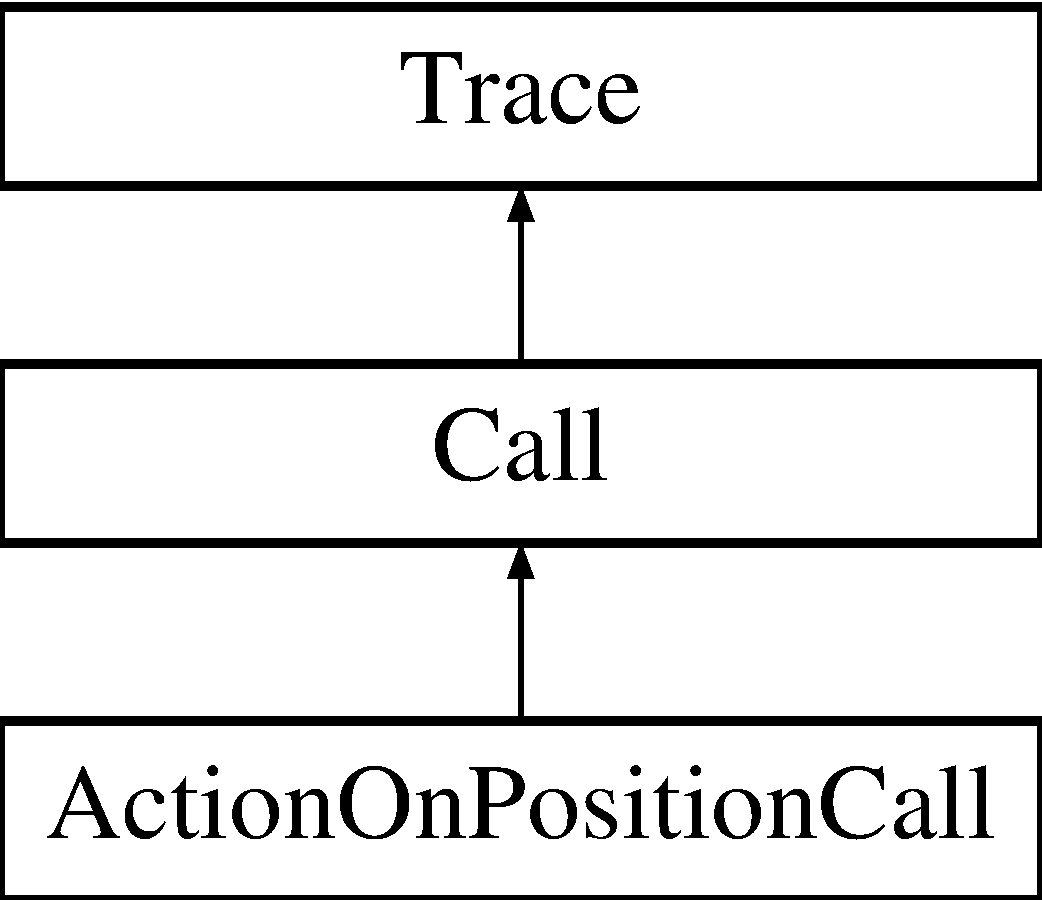
\includegraphics[height=3.000000cm]{class_action_on_position_call}
\end{center}
\end{figure}
\subsection*{Public Member Functions}
\begin{DoxyCompactItemize}
\item 
\hyperlink{class_action_on_position_call_aee0a62cf084437f5f1a50657ed2c7b8a}{Action\+On\+Position\+Call} (\hyperlink{class_call_ade833a08ce215aaa4121102f3448c898}{Error\+Type} \hyperlink{class_call_a206f6150a8038fda48c17c2c7421aed1}{error}, int unit\+Id, int unit\+Type, int action, float x, float y)
\item 
\hyperlink{class_action_on_position_call_a9a87e633b34888a0ae3ba0514628c3f7}{Action\+On\+Position\+Call} (const \hyperlink{class_action_on_position_call}{Action\+On\+Position\+Call} $\ast$c)
\item 
virtual \hyperlink{class_trace_a9c58e523529fc8a03fb6acf3eef86150}{Trace\+::sp\+\_\+trace} \hyperlink{class_action_on_position_call_aa755b6dbfcbd7efd47251556381f6bc3}{clone} () const 
\begin{DoxyCompactList}\small\item\em Clonage d\textquotesingle{}un appel. \end{DoxyCompactList}\end{DoxyCompactItemize}
\subsection*{Additional Inherited Members}


\subsection{Detailed Description}


Definition at line 596 of file Call\+Def.\+h.



\subsection{Constructor \& Destructor Documentation}
\index{Action\+On\+Position\+Call@{Action\+On\+Position\+Call}!Action\+On\+Position\+Call@{Action\+On\+Position\+Call}}
\index{Action\+On\+Position\+Call@{Action\+On\+Position\+Call}!Action\+On\+Position\+Call@{Action\+On\+Position\+Call}}
\subsubsection[{\texorpdfstring{Action\+On\+Position\+Call(\+Error\+Type error, int unit\+Id, int unit\+Type, int action, float x, float y)}{ActionOnPositionCall(ErrorType error, int unitId, int unitType, int action, float x, float y)}}]{\setlength{\rightskip}{0pt plus 5cm}Action\+On\+Position\+Call\+::\+Action\+On\+Position\+Call (
\begin{DoxyParamCaption}
\item[{{\bf Error\+Type}}]{error, }
\item[{int}]{unit\+Id, }
\item[{int}]{unit\+Type, }
\item[{int}]{action, }
\item[{float}]{x, }
\item[{float}]{y}
\end{DoxyParamCaption}
)\hspace{0.3cm}{\ttfamily [inline]}}\hypertarget{class_action_on_position_call_aee0a62cf084437f5f1a50657ed2c7b8a}{}\label{class_action_on_position_call_aee0a62cf084437f5f1a50657ed2c7b8a}


Definition at line 600 of file Call\+Def.\+h.

\index{Action\+On\+Position\+Call@{Action\+On\+Position\+Call}!Action\+On\+Position\+Call@{Action\+On\+Position\+Call}}
\index{Action\+On\+Position\+Call@{Action\+On\+Position\+Call}!Action\+On\+Position\+Call@{Action\+On\+Position\+Call}}
\subsubsection[{\texorpdfstring{Action\+On\+Position\+Call(const Action\+On\+Position\+Call $\ast$c)}{ActionOnPositionCall(const ActionOnPositionCall *c)}}]{\setlength{\rightskip}{0pt plus 5cm}Action\+On\+Position\+Call\+::\+Action\+On\+Position\+Call (
\begin{DoxyParamCaption}
\item[{const {\bf Action\+On\+Position\+Call} $\ast$}]{c}
\end{DoxyParamCaption}
)\hspace{0.3cm}{\ttfamily [inline]}}\hypertarget{class_action_on_position_call_a9a87e633b34888a0ae3ba0514628c3f7}{}\label{class_action_on_position_call_a9a87e633b34888a0ae3ba0514628c3f7}


Definition at line 607 of file Call\+Def.\+h.



\subsection{Member Function Documentation}
\index{Action\+On\+Position\+Call@{Action\+On\+Position\+Call}!clone@{clone}}
\index{clone@{clone}!Action\+On\+Position\+Call@{Action\+On\+Position\+Call}}
\subsubsection[{\texorpdfstring{clone() const }{clone() const }}]{\setlength{\rightskip}{0pt plus 5cm}virtual {\bf Trace\+::sp\+\_\+trace} Action\+On\+Position\+Call\+::clone (
\begin{DoxyParamCaption}
{}
\end{DoxyParamCaption}
) const\hspace{0.3cm}{\ttfamily [inline]}, {\ttfamily [virtual]}}\hypertarget{class_action_on_position_call_aa755b6dbfcbd7efd47251556381f6bc3}{}\label{class_action_on_position_call_aa755b6dbfcbd7efd47251556381f6bc3}


Clonage d\textquotesingle{}un appel. 

\begin{DoxyReturn}{Returns}
une copie de l\textquotesingle{}objet \hyperlink{class_call}{Call}. 
\end{DoxyReturn}


Implements \hyperlink{class_call_ab3bf0965d35eb1e97ecddaf2d3978e9b}{Call}.



Definition at line 615 of file Call\+Def.\+h.



The documentation for this class was generated from the following file\+:\begin{DoxyCompactItemize}
\item 
C\+:/\+Users/\+Stephane/\+Desktop/mocahteam/\+Prog\+And\+Play/pp/traces/src/\hyperlink{_call_def_8h}{Call\+Def.\+h}\end{DoxyCompactItemize}

\hypertarget{class_action_on_unit_call}{}\section{Action\+On\+Unit\+Call Class Reference}
\label{class_action_on_unit_call}\index{Action\+On\+Unit\+Call@{Action\+On\+Unit\+Call}}


{\ttfamily \#include $<$Call\+Def.\+h$>$}

Inheritance diagram for Action\+On\+Unit\+Call\+:\begin{figure}[H]
\begin{center}
\leavevmode
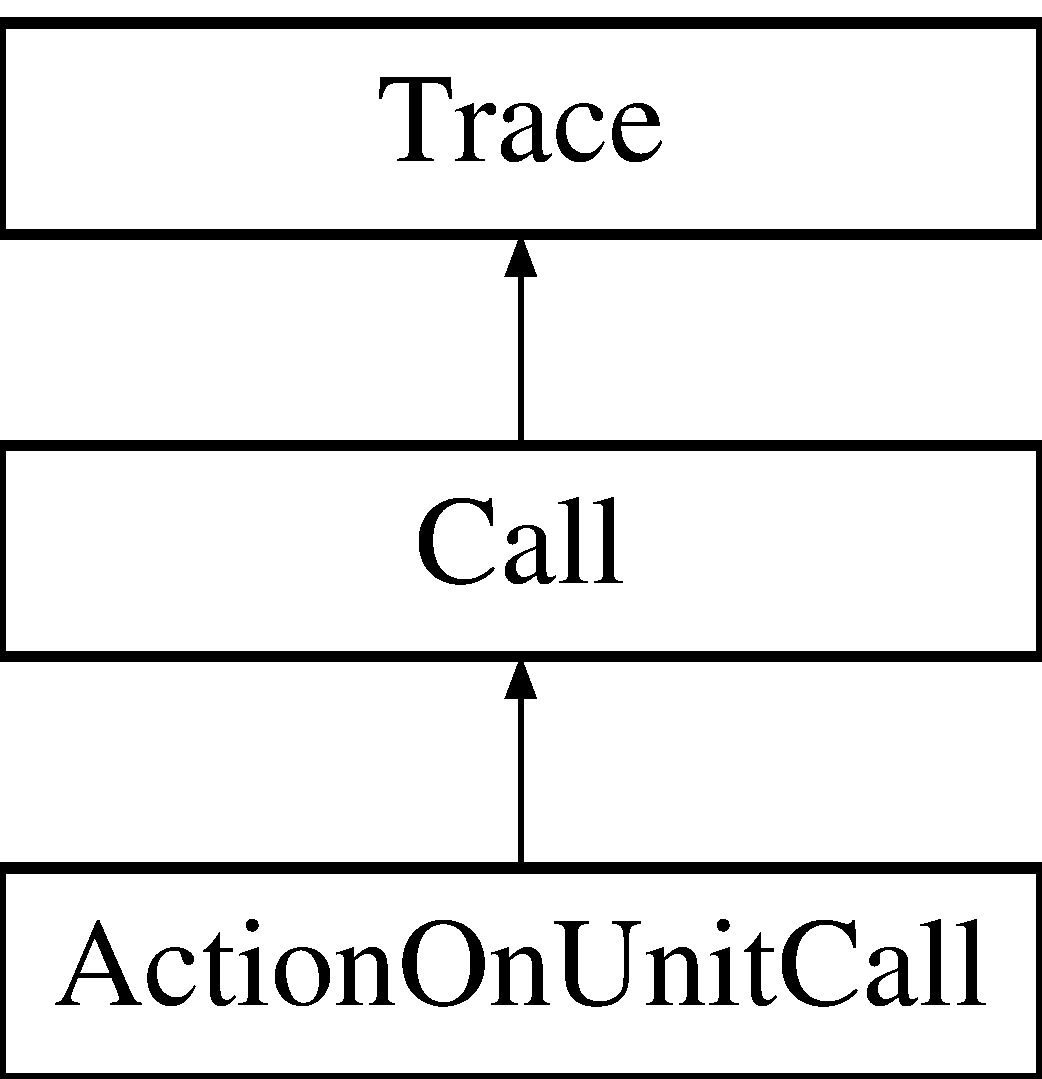
\includegraphics[height=3.000000cm]{class_action_on_unit_call}
\end{center}
\end{figure}
\subsection*{Public Member Functions}
\begin{DoxyCompactItemize}
\item 
\hyperlink{class_action_on_unit_call_acb61630fce1f24fee92c07fa291562f3}{Action\+On\+Unit\+Call} (\hyperlink{class_call_ade833a08ce215aaa4121102f3448c898}{Error\+Type} \hyperlink{class_call_a206f6150a8038fda48c17c2c7421aed1}{error}, int unit\+Id, int unit\+Type, int action, int target\+Id, int target\+Type)
\item 
\hyperlink{class_action_on_unit_call_a89332928b84f6a14a4cc558de2f73f86}{Action\+On\+Unit\+Call} (const \hyperlink{class_action_on_unit_call}{Action\+On\+Unit\+Call} $\ast$c)
\item 
virtual \hyperlink{class_trace_a9c58e523529fc8a03fb6acf3eef86150}{Trace\+::sp\+\_\+trace} \hyperlink{class_action_on_unit_call_ab127ed211f2b34f476cd0f4ef20d6057}{clone} () const 
\begin{DoxyCompactList}\small\item\em Clonage d\textquotesingle{}un appel. \end{DoxyCompactList}\end{DoxyCompactItemize}
\subsection*{Additional Inherited Members}


\subsection{Detailed Description}


Definition at line 493 of file Call\+Def.\+h.



\subsection{Constructor \& Destructor Documentation}
\index{Action\+On\+Unit\+Call@{Action\+On\+Unit\+Call}!Action\+On\+Unit\+Call@{Action\+On\+Unit\+Call}}
\index{Action\+On\+Unit\+Call@{Action\+On\+Unit\+Call}!Action\+On\+Unit\+Call@{Action\+On\+Unit\+Call}}
\subsubsection[{\texorpdfstring{Action\+On\+Unit\+Call(\+Error\+Type error, int unit\+Id, int unit\+Type, int action, int target\+Id, int target\+Type)}{ActionOnUnitCall(ErrorType error, int unitId, int unitType, int action, int targetId, int targetType)}}]{\setlength{\rightskip}{0pt plus 5cm}Action\+On\+Unit\+Call\+::\+Action\+On\+Unit\+Call (
\begin{DoxyParamCaption}
\item[{{\bf Error\+Type}}]{error, }
\item[{int}]{unit\+Id, }
\item[{int}]{unit\+Type, }
\item[{int}]{action, }
\item[{int}]{target\+Id, }
\item[{int}]{target\+Type}
\end{DoxyParamCaption}
)\hspace{0.3cm}{\ttfamily [inline]}}\hypertarget{class_action_on_unit_call_acb61630fce1f24fee92c07fa291562f3}{}\label{class_action_on_unit_call_acb61630fce1f24fee92c07fa291562f3}


Definition at line 497 of file Call\+Def.\+h.

\index{Action\+On\+Unit\+Call@{Action\+On\+Unit\+Call}!Action\+On\+Unit\+Call@{Action\+On\+Unit\+Call}}
\index{Action\+On\+Unit\+Call@{Action\+On\+Unit\+Call}!Action\+On\+Unit\+Call@{Action\+On\+Unit\+Call}}
\subsubsection[{\texorpdfstring{Action\+On\+Unit\+Call(const Action\+On\+Unit\+Call $\ast$c)}{ActionOnUnitCall(const ActionOnUnitCall *c)}}]{\setlength{\rightskip}{0pt plus 5cm}Action\+On\+Unit\+Call\+::\+Action\+On\+Unit\+Call (
\begin{DoxyParamCaption}
\item[{const {\bf Action\+On\+Unit\+Call} $\ast$}]{c}
\end{DoxyParamCaption}
)\hspace{0.3cm}{\ttfamily [inline]}}\hypertarget{class_action_on_unit_call_a89332928b84f6a14a4cc558de2f73f86}{}\label{class_action_on_unit_call_a89332928b84f6a14a4cc558de2f73f86}


Definition at line 504 of file Call\+Def.\+h.



\subsection{Member Function Documentation}
\index{Action\+On\+Unit\+Call@{Action\+On\+Unit\+Call}!clone@{clone}}
\index{clone@{clone}!Action\+On\+Unit\+Call@{Action\+On\+Unit\+Call}}
\subsubsection[{\texorpdfstring{clone() const }{clone() const }}]{\setlength{\rightskip}{0pt plus 5cm}virtual {\bf Trace\+::sp\+\_\+trace} Action\+On\+Unit\+Call\+::clone (
\begin{DoxyParamCaption}
{}
\end{DoxyParamCaption}
) const\hspace{0.3cm}{\ttfamily [inline]}, {\ttfamily [virtual]}}\hypertarget{class_action_on_unit_call_ab127ed211f2b34f476cd0f4ef20d6057}{}\label{class_action_on_unit_call_ab127ed211f2b34f476cd0f4ef20d6057}


Clonage d\textquotesingle{}un appel. 

\begin{DoxyReturn}{Returns}
une copie de l\textquotesingle{}objet \hyperlink{class_call}{Call}. 
\end{DoxyReturn}


Implements \hyperlink{class_call_ab3bf0965d35eb1e97ecddaf2d3978e9b}{Call}.



Definition at line 512 of file Call\+Def.\+h.



The documentation for this class was generated from the following file\+:\begin{DoxyCompactItemize}
\item 
C\+:/\+Users/\+Stephane/\+Desktop/mocahteam/\+Prog\+And\+Play/pp/traces/src/\hyperlink{_call_def_8h}{Call\+Def.\+h}\end{DoxyCompactItemize}

\hypertarget{class_call}{}\section{Call Class Reference}
\label{class_call}\index{Call@{Call}}


Classe abstraite héritant de \hyperlink{class_trace}{Trace}. Cette classe sert de classe mère pour toutes les classes définies dans le fichier \hyperlink{_call_def_8h}{Call\+Def.\+h}.  




{\ttfamily \#include $<$Call.\+h$>$}

Inheritance diagram for Call\+:\begin{figure}[H]
\begin{center}
\leavevmode
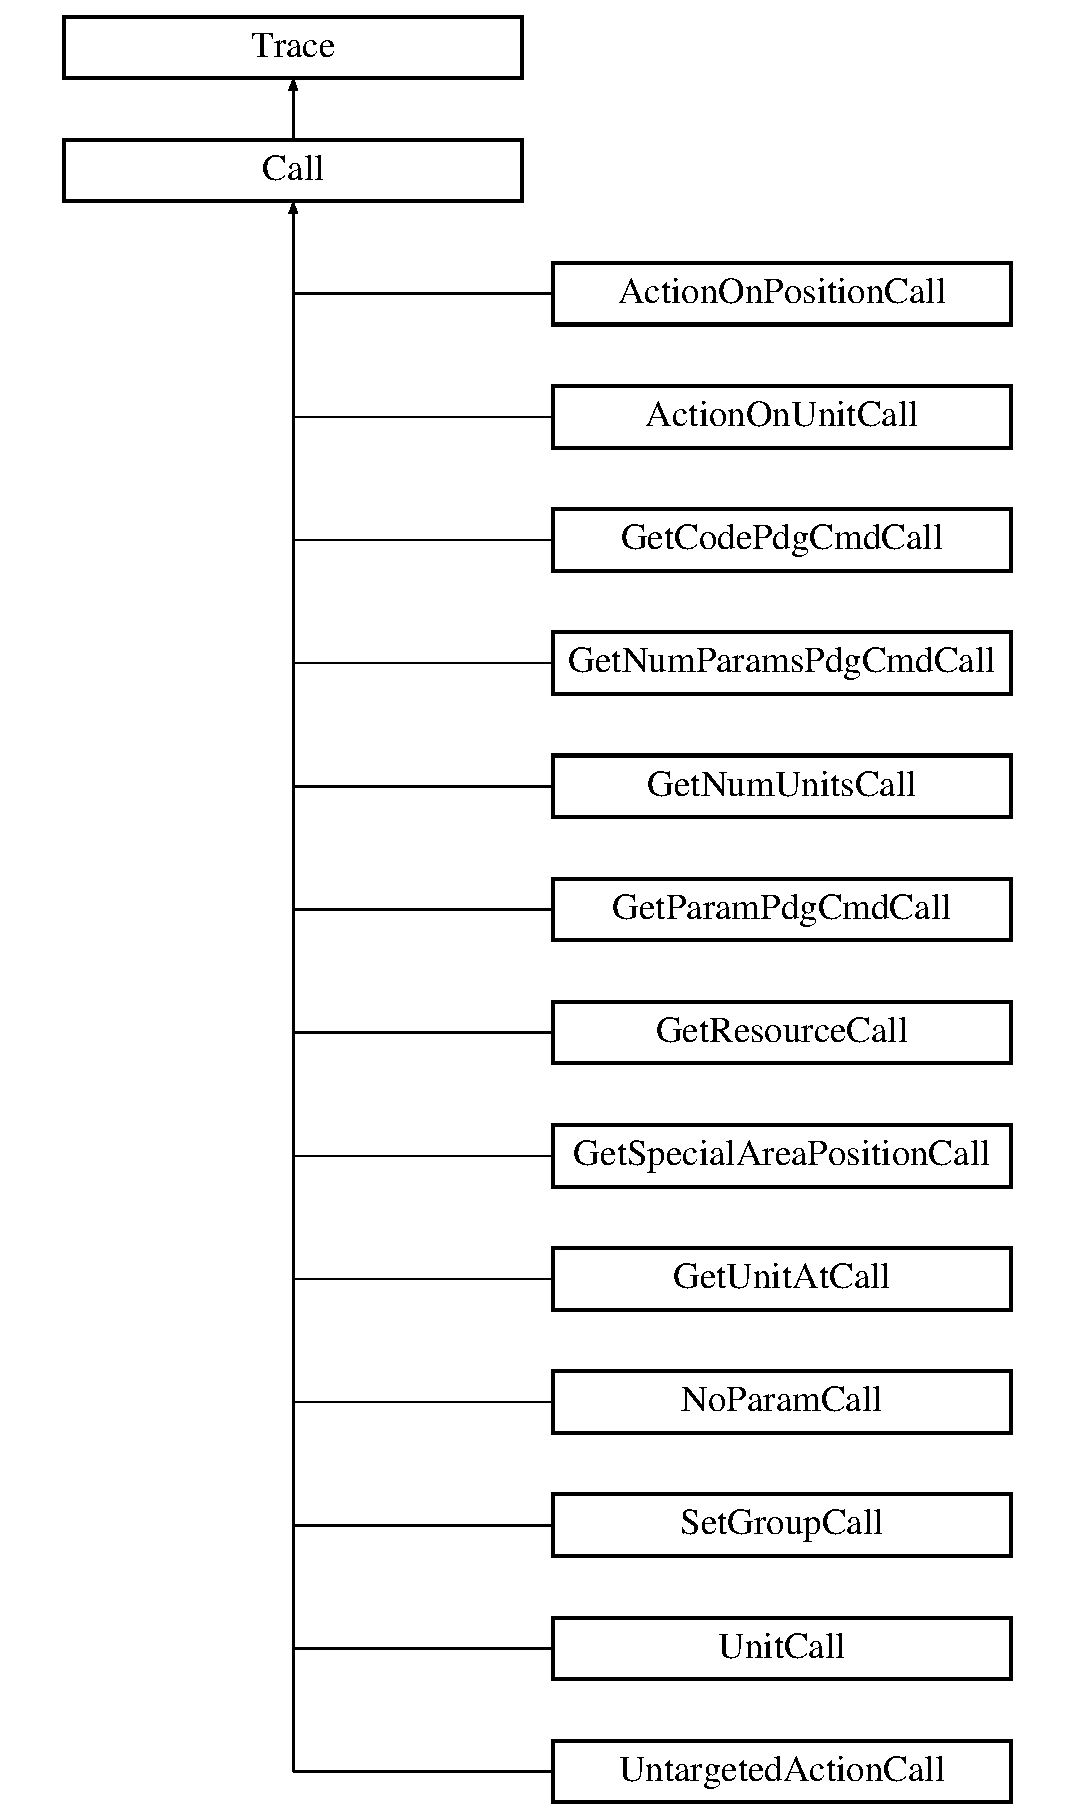
\includegraphics[height=12.000000cm]{class_call}
\end{center}
\end{figure}
\subsection*{Public Types}
\begin{DoxyCompactItemize}
\item 
enum \hyperlink{class_call_ade833a08ce215aaa4121102f3448c898}{Error\+Type} \{ \\*
\hyperlink{class_call_ade833a08ce215aaa4121102f3448c898a672dcb94435dc8e1e9a33ae581328ff4}{N\+O\+NE} = -\/1, 
\hyperlink{class_call_ade833a08ce215aaa4121102f3448c898a6683d72305e4eb207a1fef960d382da2}{O\+U\+T\+\_\+\+O\+F\+\_\+\+R\+A\+N\+GE}, 
\hyperlink{class_call_ade833a08ce215aaa4121102f3448c898afbdbbeb758c8827116fcd1b22da74d98}{W\+R\+O\+N\+G\+\_\+\+C\+O\+A\+L\+I\+T\+I\+ON}, 
\hyperlink{class_call_ade833a08ce215aaa4121102f3448c898a92cfb2a9e7bb655e5238e59cd2e77c95}{W\+R\+O\+N\+G\+\_\+\+U\+N\+IT}, 
\\*
\hyperlink{class_call_ade833a08ce215aaa4121102f3448c898a737864f300ae8be2eae56bcd4b71072d}{W\+R\+O\+N\+G\+\_\+\+T\+A\+R\+G\+ET}, 
\hyperlink{class_call_ade833a08ce215aaa4121102f3448c898ab5c4229f384c869c390469e0edc2c335}{W\+R\+O\+N\+G\+\_\+\+P\+O\+S\+I\+T\+I\+ON}
 \}\begin{DoxyCompactList}\small\item\em Enumération utilisée pour connaître le type d\textquotesingle{}erreur associé à l\textquotesingle{}objet \hyperlink{class_call}{Call}. \end{DoxyCompactList}
\item 
typedef boost\+::shared\+\_\+ptr$<$ \hyperlink{class_call}{Call} $>$ \hyperlink{class_call_a4c0609ade3e9bd1366499e2f64f6e0a2}{sp\+\_\+call}
\item 
typedef std\+::vector$<$ \hyperlink{class_call_a4c0609ade3e9bd1366499e2f64f6e0a2}{sp\+\_\+call} $>$ \hyperlink{class_call_aa446a4316c03fb722ab10d0e1da33643}{call\+\_\+vector}
\end{DoxyCompactItemize}
\subsection*{Public Member Functions}
\begin{DoxyCompactItemize}
\item 
\hyperlink{class_call_a5c9ce1d9165652dfc34a0a471a036c5e}{Call} (std\+::string \hyperlink{class_call_ad6b8343d530798fdb48407b3f2489ae7}{label}, \hyperlink{class_call_ade833a08ce215aaa4121102f3448c898}{Error\+Type} \hyperlink{class_call_a206f6150a8038fda48c17c2c7421aed1}{error}, std\+::string \hyperlink{class_trace_a4835dcfa7da5d4c971e8f7d6860acb09}{info}=\char`\"{}\char`\"{})
\begin{DoxyCompactList}\small\item\em Constructeur principal de la classe \hyperlink{class_call}{Call}. \end{DoxyCompactList}\item 
\hyperlink{class_call_ac67647d4a7daa45d0dcd5f971f376fc6}{Call} (const \hyperlink{class_call}{Call} $\ast$c)
\item 
virtual unsigned int \hyperlink{class_call_ac94d8a7498716a0131a731963f035905}{length} () const 
\begin{DoxyCompactList}\small\item\em Récupération de la longueur (l\textquotesingle{}espace occupé dans un vecteur de traces) d\textquotesingle{}un appel. \end{DoxyCompactList}\item 
virtual bool \hyperlink{class_call_a63f6986cf6a599a25705cf05687f6412}{operator==} (\hyperlink{class_trace}{Trace} $\ast$t) const 
\begin{DoxyCompactList}\small\item\em Comparaison de l\textquotesingle{}objet \hyperlink{class_call}{Call} avec une trace {\ttfamily t}. \end{DoxyCompactList}\item 
virtual void \hyperlink{class_call_a9fa2498f2e58dd9efe627a69dfdfb7f0}{filter\+Call} (const \hyperlink{class_call}{Call} $\ast$c)
\begin{DoxyCompactList}\small\item\em Détection des paramètres non robustes. \end{DoxyCompactList}\item 
virtual void \hyperlink{class_call_a397f37a434fc1b186ea3460d0c21ff43}{display} (std\+::ostream \&os=std\+::cout) const 
\begin{DoxyCompactList}\small\item\em Affichage des informations de l\textquotesingle{}objet \hyperlink{class_call}{Call}. \end{DoxyCompactList}\item 
virtual \hyperlink{class_trace_a9c58e523529fc8a03fb6acf3eef86150}{Trace\+::sp\+\_\+trace} \hyperlink{class_call_ab3bf0965d35eb1e97ecddaf2d3978e9b}{clone} () const  =0
\begin{DoxyCompactList}\small\item\em Clonage d\textquotesingle{}un appel. \end{DoxyCompactList}\item 
virtual std\+::string \hyperlink{class_call_af77d25bd64b8a89750950c872cec1a8c}{get\+Params} () const  =0
\begin{DoxyCompactList}\small\item\em Récupération des paramètres de l\textquotesingle{}appel sous forme de chaîne de caractères. \end{DoxyCompactList}\item 
virtual std\+::string \hyperlink{class_call_a3b0d9700a627280d86af88ef128f2f83}{get\+Readable\+Params} () const  =0
\begin{DoxyCompactList}\small\item\em Récupération des paramètres de l\textquotesingle{}appel sous forme de chaîne de caractères. \end{DoxyCompactList}\item 
virtual std\+::vector$<$ std\+::string $>$ \hyperlink{class_call_a0c1f026fe71ef9faaab3bfdf6e954f40}{get\+List\+Id\+Wrong\+Params} (\hyperlink{class_call}{Call} $\ast$c=N\+U\+LL) const 
\begin{DoxyCompactList}\small\item\em Récupération des identifiants des paramètres non conformes. \end{DoxyCompactList}\item 
double \hyperlink{class_call_aa184f73d80fafba5e1a8c78007bfd01a}{get\+Edit\+Distance} (const \hyperlink{class_call}{Call} $\ast$c) const 
\begin{DoxyCompactList}\small\item\em Calcul de la distance entre deux appels. \end{DoxyCompactList}\item 
std\+::string \hyperlink{class_call_a42f1632ea1ae777b469a5ce60bce6557}{get\+Label} () const 
\begin{DoxyCompactList}\small\item\em Getter pour la variable {\ttfamily label}. \end{DoxyCompactList}\item 
\hyperlink{class_call_ade833a08ce215aaa4121102f3448c898}{Error\+Type} \hyperlink{class_call_a7d624f62e2e404da13441057bb0b7807}{get\+Error} () const 
\begin{DoxyCompactList}\small\item\em Getter pour la variable {\ttfamily error}. \end{DoxyCompactList}\item 
bool \hyperlink{class_call_a60fcad7a31734fe08b1d30003099597d}{add\+Return\+Code} (float code)
\begin{DoxyCompactList}\small\item\em Ajout d\textquotesingle{}une valeur dans le tableau {\ttfamily ret} contenant les codes de retour de l\textquotesingle{}appel. \end{DoxyCompactList}\item 
std\+::string \hyperlink{class_call_a16aa36fdd27ccbbe7102e92b10eeb455}{get\+Return} () const 
\begin{DoxyCompactList}\small\item\em Récupération des codes de retour sous forme de chaîne de caractères. \end{DoxyCompactList}\item 
bool \hyperlink{class_call_a55acd6e34cc1510d6fabc354a1883c8e}{compare\+Return} (const \hyperlink{class_call}{Call} $\ast$c) const 
\begin{DoxyCompactList}\small\item\em Comparaison des codes de retour entre deux appels. \end{DoxyCompactList}\item 
void \hyperlink{class_call_aacee3123aaa6a75fb52b360cf9635dc3}{set\+Return} ()
\begin{DoxyCompactList}\small\item\em Mise à -\/1 de {\ttfamily ind\+\_\+ret}. \end{DoxyCompactList}\item 
bool \hyperlink{class_call_a4d93216142746c833503dec59c07c11c}{has\+Return} () const 
\begin{DoxyCompactList}\small\item\em Indique si l\textquotesingle{}appel a un retour. \end{DoxyCompactList}\end{DoxyCompactItemize}
\subsection*{Static Public Member Functions}
\begin{DoxyCompactItemize}
\item 
{\footnotesize template$<$typename E $>$ }\\static E \hyperlink{class_call_a46a8f56e18b25a36d951c3d59ec3211a}{get\+Enum\+Type} (const char $\ast$ch, const char $\ast$$\ast$arr)
\begin{DoxyCompactList}\small\item\em Récupération de la valeur d\textquotesingle{}une énumération à partir d\textquotesingle{}une chaîne de caractères. \end{DoxyCompactList}\item 
{\footnotesize template$<$typename E $>$ }\\static const char $\ast$ \hyperlink{class_call_a1df0e032b2cb618b6b92e8f86c3704a9}{get\+Enum\+Label} (E e, const char $\ast$$\ast$arr)
\begin{DoxyCompactList}\small\item\em Récupération d\textquotesingle{}une chaîne de caractères à partir de la valeur d\textquotesingle{}une énumération. \end{DoxyCompactList}\end{DoxyCompactItemize}
\subsection*{Static Public Attributes}
\begin{DoxyCompactItemize}
\item 
static const char $\ast$ \hyperlink{class_call_a9b4594fe997fce2b0155af42d47af07a}{errors\+Arr} \mbox{[}$\,$\mbox{]} = \{\char`\"{}out\+\_\+of\+\_\+range\char`\"{}, \char`\"{}wrong\+\_\+coalition\char`\"{}, \char`\"{}wrong\+\_\+unit\char`\"{}, \char`\"{}wrong\+\_\+target\char`\"{}, \char`\"{}wrong\+\_\+position\char`\"{}, N\+U\+LL\}
\item 
static const char $\ast$ \hyperlink{class_call_a69386ad6806856e50ad09edf31998dc2}{coalitions\+Arr} \mbox{[}$\,$\mbox{]} = \{\char`\"{}M\+Y\+\_\+\+C\+O\+A\+L\+I\+T\+I\+ON\char`\"{}, \char`\"{}A\+L\+L\+Y\+\_\+\+C\+O\+A\+L\+I\+T\+I\+ON\char`\"{}, \char`\"{}E\+N\+E\+M\+Y\+\_\+\+C\+O\+A\+L\+I\+T\+I\+ON\char`\"{}, N\+U\+LL\}
\item 
static const char $\ast$ \hyperlink{class_call_a502f84377bff9a869d6c0349408a8cd1}{no\+Param\+Call\+Labels\+Arr} \mbox{[}$\,$\mbox{]} = \{\char`\"{}P\+P\+\_\+\+Open\char`\"{}, \char`\"{}P\+P\+\_\+\+Close\char`\"{}, \char`\"{}P\+P\+\_\+\+Is\+Game\+Over\char`\"{}, \char`\"{}P\+P\+\_\+\+Get\+Map\+Size\char`\"{}, \char`\"{}P\+P\+\_\+\+Get\+Start\+Position\char`\"{}, \char`\"{}P\+P\+\_\+\+Get\+Num\+Special\+Areas\char`\"{}, N\+U\+LL\}
\item 
static const char $\ast$ \hyperlink{class_call_a7f62a26228ad25563c7dfbacda6f9759}{unit\+Call\+Labels\+Arr} \mbox{[}$\,$\mbox{]} = \{\char`\"{}P\+P\+\_\+\+Unit\+\_\+\+Get\+Coalition\char`\"{}, \char`\"{}P\+P\+\_\+\+Unit\+\_\+\+Get\+Type\char`\"{}, \char`\"{}P\+P\+\_\+\+Unit\+\_\+\+Get\+Position\char`\"{}, \char`\"{}P\+P\+\_\+\+Unit\+\_\+\+Get\+Health\char`\"{}, \char`\"{}P\+P\+\_\+\+Unit\+\_\+\+Get\+Max\+Health\char`\"{}, \char`\"{}P\+P\+\_\+\+Unit\+\_\+\+Get\+Pending\+Commands\char`\"{}, \char`\"{}P\+P\+\_\+\+Unit\+\_\+\+Get\+Group\char`\"{}, \char`\"{}P\+P\+\_\+\+Unit\+\_\+\+Get\+Num\+Pdg\+Cmds\char`\"{}, N\+U\+LL\}
\item 
static \hyperlink{class_params_map}{Params\+Map} \hyperlink{class_call_ab91ad28c9446ceec253123d66b23f81c}{params\+Map}
\end{DoxyCompactItemize}
\subsection*{Protected Member Functions}
\begin{DoxyCompactItemize}
\item 
virtual bool \hyperlink{class_call_a48f59d92851fd5802ace768dc9470564}{compare} (const \hyperlink{class_call}{Call} $\ast$c) const  =0
\begin{DoxyCompactList}\small\item\em Comparaison entre deux appels. \end{DoxyCompactList}\item 
virtual void \hyperlink{class_call_acd4b5ce39b8ab5850321594dea288940}{filter} (const \hyperlink{class_call}{Call} $\ast$c)=0
\begin{DoxyCompactList}\small\item\em Détection des paramètres non robustes. \end{DoxyCompactList}\item 
virtual std\+::pair$<$ int, int $>$ \hyperlink{class_call_a79e000ddc3d6c863e28d601e417b096f}{distance} (const \hyperlink{class_call}{Call} $\ast$c) const  =0
\begin{DoxyCompactList}\small\item\em Détermination de la distance entre deux appels. \end{DoxyCompactList}\item 
virtual std\+::vector$<$ std\+::string $>$ \hyperlink{class_call_a4ca5c037197ed0391119ac7be3eb14c6}{id\+\_\+wrong\+\_\+params} (\hyperlink{class_call}{Call} $\ast$c) const  =0
\end{DoxyCompactItemize}
\subsection*{Protected Attributes}
\begin{DoxyCompactItemize}
\item 
std\+::string \hyperlink{class_call_ad6b8343d530798fdb48407b3f2489ae7}{label}
\item 
\hyperlink{class_call_ade833a08ce215aaa4121102f3448c898}{Error\+Type} \hyperlink{class_call_a206f6150a8038fda48c17c2c7421aed1}{error}
\item 
int \hyperlink{class_call_ac61426df38580506f015d44c687c2ee8}{ind\+\_\+ret}
\item 
float \hyperlink{class_call_a634f1033a7d282e03578a3d0fd2823f8}{ret} \mbox{[}\hyperlink{_call_8h_a92280872d50a2c64ffe1acbc6c88dfff}{M\+A\+X\+\_\+\+S\+I\+Z\+E\+\_\+\+P\+A\+R\+A\+MS}\mbox{]}
\end{DoxyCompactItemize}
\subsection*{Additional Inherited Members}


\subsection{Detailed Description}
Classe abstraite héritant de \hyperlink{class_trace}{Trace}. Cette classe sert de classe mère pour toutes les classes définies dans le fichier \hyperlink{_call_def_8h}{Call\+Def.\+h}. 

Definition at line 121 of file Call.\+h.



\subsection{Member Typedef Documentation}
\index{Call@{Call}!call\+\_\+vector@{call\+\_\+vector}}
\index{call\+\_\+vector@{call\+\_\+vector}!Call@{Call}}
\subsubsection[{\texorpdfstring{call\+\_\+vector}{call_vector}}]{\setlength{\rightskip}{0pt plus 5cm}typedef std\+::vector$<${\bf sp\+\_\+call}$>$ {\bf Call\+::call\+\_\+vector}}\hypertarget{class_call_aa446a4316c03fb722ab10d0e1da33643}{}\label{class_call_aa446a4316c03fb722ab10d0e1da33643}


Definition at line 130 of file Call.\+h.

\index{Call@{Call}!sp\+\_\+call@{sp\+\_\+call}}
\index{sp\+\_\+call@{sp\+\_\+call}!Call@{Call}}
\subsubsection[{\texorpdfstring{sp\+\_\+call}{sp_call}}]{\setlength{\rightskip}{0pt plus 5cm}typedef boost\+::shared\+\_\+ptr$<${\bf Call}$>$ {\bf Call\+::sp\+\_\+call}}\hypertarget{class_call_a4c0609ade3e9bd1366499e2f64f6e0a2}{}\label{class_call_a4c0609ade3e9bd1366499e2f64f6e0a2}
Définition du type pointeur intelligent vers un objet \hyperlink{class_call}{Call}. 

Definition at line 128 of file Call.\+h.



\subsection{Member Enumeration Documentation}
\index{Call@{Call}!Error\+Type@{Error\+Type}}
\index{Error\+Type@{Error\+Type}!Call@{Call}}
\subsubsection[{\texorpdfstring{Error\+Type}{ErrorType}}]{\setlength{\rightskip}{0pt plus 5cm}enum {\bf Call\+::\+Error\+Type}}\hypertarget{class_call_ade833a08ce215aaa4121102f3448c898}{}\label{class_call_ade833a08ce215aaa4121102f3448c898}


Enumération utilisée pour connaître le type d\textquotesingle{}erreur associé à l\textquotesingle{}objet \hyperlink{class_call}{Call}. 

\begin{Desc}
\item[Enumerator]\par
\begin{description}
\index{N\+O\+NE@{N\+O\+NE}!Call@{Call}}\index{Call@{Call}!N\+O\+NE@{N\+O\+NE}}\item[{\em 
N\+O\+NE\hypertarget{class_call_ade833a08ce215aaa4121102f3448c898a672dcb94435dc8e1e9a33ae581328ff4}{}\label{class_call_ade833a08ce215aaa4121102f3448c898a672dcb94435dc8e1e9a33ae581328ff4}
}]\index{O\+U\+T\+\_\+\+O\+F\+\_\+\+R\+A\+N\+GE@{O\+U\+T\+\_\+\+O\+F\+\_\+\+R\+A\+N\+GE}!Call@{Call}}\index{Call@{Call}!O\+U\+T\+\_\+\+O\+F\+\_\+\+R\+A\+N\+GE@{O\+U\+T\+\_\+\+O\+F\+\_\+\+R\+A\+N\+GE}}\item[{\em 
O\+U\+T\+\_\+\+O\+F\+\_\+\+R\+A\+N\+GE\hypertarget{class_call_ade833a08ce215aaa4121102f3448c898a6683d72305e4eb207a1fef960d382da2}{}\label{class_call_ade833a08ce215aaa4121102f3448c898a6683d72305e4eb207a1fef960d382da2}
}]\index{W\+R\+O\+N\+G\+\_\+\+C\+O\+A\+L\+I\+T\+I\+ON@{W\+R\+O\+N\+G\+\_\+\+C\+O\+A\+L\+I\+T\+I\+ON}!Call@{Call}}\index{Call@{Call}!W\+R\+O\+N\+G\+\_\+\+C\+O\+A\+L\+I\+T\+I\+ON@{W\+R\+O\+N\+G\+\_\+\+C\+O\+A\+L\+I\+T\+I\+ON}}\item[{\em 
W\+R\+O\+N\+G\+\_\+\+C\+O\+A\+L\+I\+T\+I\+ON\hypertarget{class_call_ade833a08ce215aaa4121102f3448c898afbdbbeb758c8827116fcd1b22da74d98}{}\label{class_call_ade833a08ce215aaa4121102f3448c898afbdbbeb758c8827116fcd1b22da74d98}
}]\index{W\+R\+O\+N\+G\+\_\+\+U\+N\+IT@{W\+R\+O\+N\+G\+\_\+\+U\+N\+IT}!Call@{Call}}\index{Call@{Call}!W\+R\+O\+N\+G\+\_\+\+U\+N\+IT@{W\+R\+O\+N\+G\+\_\+\+U\+N\+IT}}\item[{\em 
W\+R\+O\+N\+G\+\_\+\+U\+N\+IT\hypertarget{class_call_ade833a08ce215aaa4121102f3448c898a92cfb2a9e7bb655e5238e59cd2e77c95}{}\label{class_call_ade833a08ce215aaa4121102f3448c898a92cfb2a9e7bb655e5238e59cd2e77c95}
}]\index{W\+R\+O\+N\+G\+\_\+\+T\+A\+R\+G\+ET@{W\+R\+O\+N\+G\+\_\+\+T\+A\+R\+G\+ET}!Call@{Call}}\index{Call@{Call}!W\+R\+O\+N\+G\+\_\+\+T\+A\+R\+G\+ET@{W\+R\+O\+N\+G\+\_\+\+T\+A\+R\+G\+ET}}\item[{\em 
W\+R\+O\+N\+G\+\_\+\+T\+A\+R\+G\+ET\hypertarget{class_call_ade833a08ce215aaa4121102f3448c898a737864f300ae8be2eae56bcd4b71072d}{}\label{class_call_ade833a08ce215aaa4121102f3448c898a737864f300ae8be2eae56bcd4b71072d}
}]\index{W\+R\+O\+N\+G\+\_\+\+P\+O\+S\+I\+T\+I\+ON@{W\+R\+O\+N\+G\+\_\+\+P\+O\+S\+I\+T\+I\+ON}!Call@{Call}}\index{Call@{Call}!W\+R\+O\+N\+G\+\_\+\+P\+O\+S\+I\+T\+I\+ON@{W\+R\+O\+N\+G\+\_\+\+P\+O\+S\+I\+T\+I\+ON}}\item[{\em 
W\+R\+O\+N\+G\+\_\+\+P\+O\+S\+I\+T\+I\+ON\hypertarget{class_call_ade833a08ce215aaa4121102f3448c898ab5c4229f384c869c390469e0edc2c335}{}\label{class_call_ade833a08ce215aaa4121102f3448c898ab5c4229f384c869c390469e0edc2c335}
}]\end{description}
\end{Desc}


Definition at line 135 of file Call.\+h.



\subsection{Constructor \& Destructor Documentation}
\index{Call@{Call}!Call@{Call}}
\index{Call@{Call}!Call@{Call}}
\subsubsection[{\texorpdfstring{Call(std\+::string label, Error\+Type error, std\+::string info="""")}{Call(std::string label, ErrorType error, std::string info="")}}]{\setlength{\rightskip}{0pt plus 5cm}Call\+::\+Call (
\begin{DoxyParamCaption}
\item[{std\+::string}]{label, }
\item[{{\bf Error\+Type}}]{error, }
\item[{std\+::string}]{info = {\ttfamily \char`\"{}\char`\"{}}}
\end{DoxyParamCaption}
)}\hypertarget{class_call_a5c9ce1d9165652dfc34a0a471a036c5e}{}\label{class_call_a5c9ce1d9165652dfc34a0a471a036c5e}


Constructeur principal de la classe \hyperlink{class_call}{Call}. 


\begin{DoxyParams}{Parameters}
{\em label} & le label de la fonction modélisée par l\textquotesingle{}objet \hyperlink{class_call}{Call}. \\
\hline
{\em error} & l\textquotesingle{}erreur survenue lors de l\textquotesingle{}appel de la fonction représentée par l\textquotesingle{}objet \hyperlink{class_call}{Call}. \\
\hline
{\em info} & le label attribué par l\textquotesingle{}expert. \\
\hline
\end{DoxyParams}


Definition at line 9 of file Call.\+cpp.

\index{Call@{Call}!Call@{Call}}
\index{Call@{Call}!Call@{Call}}
\subsubsection[{\texorpdfstring{Call(const Call $\ast$c)}{Call(const Call *c)}}]{\setlength{\rightskip}{0pt plus 5cm}Call\+::\+Call (
\begin{DoxyParamCaption}
\item[{const {\bf Call} $\ast$}]{c}
\end{DoxyParamCaption}
)}\hypertarget{class_call_ac67647d4a7daa45d0dcd5f971f376fc6}{}\label{class_call_ac67647d4a7daa45d0dcd5f971f376fc6}
Constructeur de la classe \hyperlink{class_call}{Call} utilisé notamment lors de la copie de l\textquotesingle{}objet. 

Definition at line 11 of file Call.\+cpp.



\subsection{Member Function Documentation}
\index{Call@{Call}!add\+Return\+Code@{add\+Return\+Code}}
\index{add\+Return\+Code@{add\+Return\+Code}!Call@{Call}}
\subsubsection[{\texorpdfstring{add\+Return\+Code(float code)}{addReturnCode(float code)}}]{\setlength{\rightskip}{0pt plus 5cm}bool Call\+::add\+Return\+Code (
\begin{DoxyParamCaption}
\item[{float}]{code}
\end{DoxyParamCaption}
)}\hypertarget{class_call_a60fcad7a31734fe08b1d30003099597d}{}\label{class_call_a60fcad7a31734fe08b1d30003099597d}


Ajout d\textquotesingle{}une valeur dans le tableau {\ttfamily ret} contenant les codes de retour de l\textquotesingle{}appel. 


\begin{DoxyParams}{Parameters}
{\em code} & \+: le code retour de l\textquotesingle{}appel à sauvegarder dans le tableau {\ttfamily ret}.\\
\hline
\end{DoxyParams}
\begin{DoxyReturn}{Returns}
vrai si la valeur a bien été sauvegardée dans {\ttfamily ret}, et faux sinon (plus de place disponible). 
\end{DoxyReturn}


Definition at line 106 of file Call.\+cpp.

\index{Call@{Call}!clone@{clone}}
\index{clone@{clone}!Call@{Call}}
\subsubsection[{\texorpdfstring{clone() const  =0}{clone() const  =0}}]{\setlength{\rightskip}{0pt plus 5cm}virtual {\bf Trace\+::sp\+\_\+trace} Call\+::clone (
\begin{DoxyParamCaption}
{}
\end{DoxyParamCaption}
) const\hspace{0.3cm}{\ttfamily [pure virtual]}}\hypertarget{class_call_ab3bf0965d35eb1e97ecddaf2d3978e9b}{}\label{class_call_ab3bf0965d35eb1e97ecddaf2d3978e9b}


Clonage d\textquotesingle{}un appel. 

\begin{DoxyReturn}{Returns}
une copie de l\textquotesingle{}objet \hyperlink{class_call}{Call}. 
\end{DoxyReturn}


Implements \hyperlink{class_trace_a0917758337e37f936713ccaf75b532f2}{Trace}.



Implemented in \hyperlink{class_get_param_pdg_cmd_call_a07b0bec23a831830746b25ca5d44b317}{Get\+Param\+Pdg\+Cmd\+Call}, \hyperlink{class_get_num_params_pdg_cmd_call_ae0633bca77530d2e3ad5bc3a68109c8f}{Get\+Num\+Params\+Pdg\+Cmd\+Call}, \hyperlink{class_get_code_pdg_cmd_call_adad7b71e06c9b81d17b02191401245f5}{Get\+Code\+Pdg\+Cmd\+Call}, \hyperlink{class_untargeted_action_call_a483d86c01a984c4b1e59e339a1f7329e}{Untargeted\+Action\+Call}, \hyperlink{class_action_on_position_call_aa755b6dbfcbd7efd47251556381f6bc3}{Action\+On\+Position\+Call}, \hyperlink{class_action_on_unit_call_ab127ed211f2b34f476cd0f4ef20d6057}{Action\+On\+Unit\+Call}, \hyperlink{class_set_group_call_ac970b30cd2a4769ec134ba451768ee64}{Set\+Group\+Call}, \hyperlink{class_unit_call_a637d309cd3d0bc05849aa7ca20eb5f89}{Unit\+Call}, \hyperlink{class_get_unit_at_call_a228108026f5f8522a6724e1183e1b6bb}{Get\+Unit\+At\+Call}, \hyperlink{class_get_num_units_call_a279250063949139d58842ae5a6b39b03}{Get\+Num\+Units\+Call}, \hyperlink{class_get_resource_call_adeda1479826fb33c27c76bd8fe711776}{Get\+Resource\+Call}, \hyperlink{class_get_special_area_position_call_ad522313dad00572f50f2a4a84e12dafd}{Get\+Special\+Area\+Position\+Call}, and \hyperlink{class_no_param_call_a8488a6947c974711af12b10f89298bf8}{No\+Param\+Call}.

\index{Call@{Call}!compare@{compare}}
\index{compare@{compare}!Call@{Call}}
\subsubsection[{\texorpdfstring{compare(const Call $\ast$c) const  =0}{compare(const Call *c) const  =0}}]{\setlength{\rightskip}{0pt plus 5cm}virtual bool Call\+::compare (
\begin{DoxyParamCaption}
\item[{const {\bf Call} $\ast$}]{c}
\end{DoxyParamCaption}
) const\hspace{0.3cm}{\ttfamily [protected]}, {\ttfamily [pure virtual]}}\hypertarget{class_call_a48f59d92851fd5802ace768dc9470564}{}\label{class_call_a48f59d92851fd5802ace768dc9470564}


Comparaison entre deux appels. 


\begin{DoxyParams}{Parameters}
{\em c} & \+: un pointeur vers l\textquotesingle{}objet \hyperlink{class_call}{Call} utilisé pour la comparaison.\\
\hline
\end{DoxyParams}
\begin{DoxyReturn}{Returns}
vrai si les deux appels sont égaux, et faux sinon.
\end{DoxyReturn}
\begin{DoxySeeAlso}{See also}
\hyperlink{class_call_a63f6986cf6a599a25705cf05687f6412}{Call\+::operator==} 
\end{DoxySeeAlso}
\index{Call@{Call}!compare\+Return@{compare\+Return}}
\index{compare\+Return@{compare\+Return}!Call@{Call}}
\subsubsection[{\texorpdfstring{compare\+Return(const Call $\ast$c) const }{compareReturn(const Call *c) const }}]{\setlength{\rightskip}{0pt plus 5cm}bool Call\+::compare\+Return (
\begin{DoxyParamCaption}
\item[{const {\bf Call} $\ast$}]{c}
\end{DoxyParamCaption}
) const}\hypertarget{class_call_a55acd6e34cc1510d6fabc354a1883c8e}{}\label{class_call_a55acd6e34cc1510d6fabc354a1883c8e}


Comparaison des codes de retour entre deux appels. 


\begin{DoxyParams}{Parameters}
{\em c} & \+: un pointeur vers l\textquotesingle{}appel utilisé pour la comparaison.\\
\hline
\end{DoxyParams}
\begin{DoxyReturn}{Returns}
vrai si le tableau {\ttfamily ret} de l\textquotesingle{}objet pointé par {\ttfamily c} est identique à celui de cet appel. 
\end{DoxyReturn}


Definition at line 114 of file Call.\+cpp.

\index{Call@{Call}!display@{display}}
\index{display@{display}!Call@{Call}}
\subsubsection[{\texorpdfstring{display(std\+::ostream \&os=std\+::cout) const }{display(std::ostream &os=std::cout) const }}]{\setlength{\rightskip}{0pt plus 5cm}void Call\+::display (
\begin{DoxyParamCaption}
\item[{std\+::ostream \&}]{os = {\ttfamily std\+:\+:cout}}
\end{DoxyParamCaption}
) const\hspace{0.3cm}{\ttfamily [virtual]}}\hypertarget{class_call_a397f37a434fc1b186ea3460d0c21ff43}{}\label{class_call_a397f37a434fc1b186ea3460d0c21ff43}


Affichage des informations de l\textquotesingle{}objet \hyperlink{class_call}{Call}. 


\begin{DoxyParams}{Parameters}
{\em os} & le flux de sortie utilisé pour l\textquotesingle{}affichage. \\
\hline
\end{DoxyParams}


Implements \hyperlink{class_trace_a4324fa45af235238ddedc2215c3d1cf0}{Trace}.



Definition at line 63 of file Call.\+cpp.

\index{Call@{Call}!distance@{distance}}
\index{distance@{distance}!Call@{Call}}
\subsubsection[{\texorpdfstring{distance(const Call $\ast$c) const  =0}{distance(const Call *c) const  =0}}]{\setlength{\rightskip}{0pt plus 5cm}virtual std\+::pair$<$int,int$>$ Call\+::distance (
\begin{DoxyParamCaption}
\item[{const {\bf Call} $\ast$}]{c}
\end{DoxyParamCaption}
) const\hspace{0.3cm}{\ttfamily [protected]}, {\ttfamily [pure virtual]}}\hypertarget{class_call_a79e000ddc3d6c863e28d601e417b096f}{}\label{class_call_a79e000ddc3d6c863e28d601e417b096f}


Détermination de la distance entre deux appels. 


\begin{DoxyParams}{Parameters}
{\em c} & \+: un pointeur vers l\textquotesingle{}objet \hyperlink{class_call}{Call} utilisé pour la comparaison.\\
\hline
\end{DoxyParams}
\begin{DoxyReturn}{Returns}
un couple d\textquotesingle{}entiers où le premier élément correspond au nombre de paramètres qui diffèrent entre les deux appels et où le second élément est le nombre de comparaisons effectués.
\end{DoxyReturn}
\begin{DoxySeeAlso}{See also}
\hyperlink{class_call_aa184f73d80fafba5e1a8c78007bfd01a}{Call\+::get\+Edit\+Distance} 
\end{DoxySeeAlso}
\index{Call@{Call}!filter@{filter}}
\index{filter@{filter}!Call@{Call}}
\subsubsection[{\texorpdfstring{filter(const Call $\ast$c)=0}{filter(const Call *c)=0}}]{\setlength{\rightskip}{0pt plus 5cm}virtual void Call\+::filter (
\begin{DoxyParamCaption}
\item[{const {\bf Call} $\ast$}]{c}
\end{DoxyParamCaption}
)\hspace{0.3cm}{\ttfamily [protected]}, {\ttfamily [pure virtual]}}\hypertarget{class_call_acd4b5ce39b8ab5850321594dea288940}{}\label{class_call_acd4b5ce39b8ab5850321594dea288940}


Détection des paramètres non robustes. 


\begin{DoxyParams}{Parameters}
{\em c} & \+: un pointeur vers l\textquotesingle{}objet \hyperlink{class_call}{Call} utilisé pour la comparaison.\\
\hline
\end{DoxyParams}
\begin{DoxySeeAlso}{See also}
\hyperlink{class_call_a9fa2498f2e58dd9efe627a69dfdfb7f0}{Call\+::filter\+Call} 
\end{DoxySeeAlso}
\index{Call@{Call}!filter\+Call@{filter\+Call}}
\index{filter\+Call@{filter\+Call}!Call@{Call}}
\subsubsection[{\texorpdfstring{filter\+Call(const Call $\ast$c)}{filterCall(const Call *c)}}]{\setlength{\rightskip}{0pt plus 5cm}void Call\+::filter\+Call (
\begin{DoxyParamCaption}
\item[{const {\bf Call} $\ast$}]{c}
\end{DoxyParamCaption}
)\hspace{0.3cm}{\ttfamily [virtual]}}\hypertarget{class_call_a9fa2498f2e58dd9efe627a69dfdfb7f0}{}\label{class_call_a9fa2498f2e58dd9efe627a69dfdfb7f0}


Détection des paramètres non robustes. 

Cette fonction est utilisée pour affecter aux paramètres non robustes de l\textquotesingle{}appel, i.\+e. ceux non pris en compte lors de la compression et dont la valeur diffère entre deux itération d\textquotesingle{}une même séquence, la valeur -\/1. Attention \+: cette fonction doit être appelée uniquement si operator==(c) renvoie vrai.


\begin{DoxyParams}{Parameters}
{\em c} & \+: un pointeur vers l\textquotesingle{}appel utilisé pour la comparaison. \\
\hline
\end{DoxyParams}


Definition at line 48 of file Call.\+cpp.

\index{Call@{Call}!get\+Edit\+Distance@{get\+Edit\+Distance}}
\index{get\+Edit\+Distance@{get\+Edit\+Distance}!Call@{Call}}
\subsubsection[{\texorpdfstring{get\+Edit\+Distance(const Call $\ast$c) const }{getEditDistance(const Call *c) const }}]{\setlength{\rightskip}{0pt plus 5cm}double Call\+::get\+Edit\+Distance (
\begin{DoxyParamCaption}
\item[{const {\bf Call} $\ast$}]{c}
\end{DoxyParamCaption}
) const}\hypertarget{class_call_aa184f73d80fafba5e1a8c78007bfd01a}{}\label{class_call_aa184f73d80fafba5e1a8c78007bfd01a}


Calcul de la distance entre deux appels. 


\begin{DoxyParams}{Parameters}
{\em c} & \+: un pointeur vers l\textquotesingle{}objet \hyperlink{class_call}{Call} dont l\textquotesingle{}on souhaite mesurer la distance avec cet appel.\\
\hline
\end{DoxyParams}
\begin{DoxyReturn}{Returns}
la distance dans l\textquotesingle{}intervalle \mbox{[}0,1\mbox{]} entre les deux appels. Si la distance est égale à 0, les deux appels sont complètement identiques. Si elle est égale à 1, les deux appels ont des labels et/ou des types d\textquotesingle{}erreur différents. 
\end{DoxyReturn}


Definition at line 31 of file Call.\+cpp.

\index{Call@{Call}!get\+Enum\+Label@{get\+Enum\+Label}}
\index{get\+Enum\+Label@{get\+Enum\+Label}!Call@{Call}}
\subsubsection[{\texorpdfstring{get\+Enum\+Label(\+E e, const char $\ast$$\ast$arr)}{getEnumLabel(E e, const char **arr)}}]{\setlength{\rightskip}{0pt plus 5cm}template$<$typename E $>$ static const char$\ast$ Call\+::get\+Enum\+Label (
\begin{DoxyParamCaption}
\item[{E}]{e, }
\item[{const char $\ast$$\ast$}]{arr}
\end{DoxyParamCaption}
)\hspace{0.3cm}{\ttfamily [inline]}, {\ttfamily [static]}}\hypertarget{class_call_a1df0e032b2cb618b6b92e8f86c3704a9}{}\label{class_call_a1df0e032b2cb618b6b92e8f86c3704a9}


Récupération d\textquotesingle{}une chaîne de caractères à partir de la valeur d\textquotesingle{}une énumération. 

On utilise l\textquotesingle{}entier associé à la valeur de l\textquotesingle{}énumération pour récupérer la chaîne de caractères contenu dans {\ttfamily arr}.


\begin{DoxyParams}{Parameters}
{\em e} & \+: la valeur de l\textquotesingle{}énumération. \\
\hline
{\em arr} & \+: le tableau de chaînes de caractères où l\textquotesingle{}on récupère la chaîne.\\
\hline
\end{DoxyParams}
\begin{DoxyReturn}{Returns}
la chaîne de caractères associée à la valeur de l\textquotesingle{}énumération si elle peut être récupérée dans {\ttfamily arr}, ou N\+U\+LL sinon.
\end{DoxyReturn}
\begin{DoxySeeAlso}{See also}
\hyperlink{class_call_a46a8f56e18b25a36d951c3d59ec3211a}{Call\+::get\+Enum\+Type} 
\end{DoxySeeAlso}


Definition at line 215 of file Call.\+h.

\index{Call@{Call}!get\+Enum\+Type@{get\+Enum\+Type}}
\index{get\+Enum\+Type@{get\+Enum\+Type}!Call@{Call}}
\subsubsection[{\texorpdfstring{get\+Enum\+Type(const char $\ast$ch, const char $\ast$$\ast$arr)}{getEnumType(const char *ch, const char **arr)}}]{\setlength{\rightskip}{0pt plus 5cm}template$<$typename E $>$ static E Call\+::get\+Enum\+Type (
\begin{DoxyParamCaption}
\item[{const char $\ast$}]{ch, }
\item[{const char $\ast$$\ast$}]{arr}
\end{DoxyParamCaption}
)\hspace{0.3cm}{\ttfamily [inline]}, {\ttfamily [static]}}\hypertarget{class_call_a46a8f56e18b25a36d951c3d59ec3211a}{}\label{class_call_a46a8f56e18b25a36d951c3d59ec3211a}


Récupération de la valeur d\textquotesingle{}une énumération à partir d\textquotesingle{}une chaîne de caractères. 

La chaîne {\ttfamily ch} est recherchée dans le tableau {\ttfamily arr} et l\textquotesingle{}indice de sa position est utilisée pour récupérér la bonne valeur d\textquotesingle{}énumération.


\begin{DoxyParams}{Parameters}
{\em ch} & \+: la chaîne de caractères. \\
\hline
{\em arr} & \+: le tableau de chaînes de caractères dans lequel {\ttfamily ch} est recherchée.\\
\hline
\end{DoxyParams}
\begin{DoxyReturn}{Returns}
la valeur de l\textquotesingle{}énumération associée à {\ttfamily ch}.
\end{DoxyReturn}
\begin{DoxySeeAlso}{See also}
\hyperlink{class_call_a1df0e032b2cb618b6b92e8f86c3704a9}{Call\+::get\+Enum\+Label} 
\end{DoxySeeAlso}


Definition at line 198 of file Call.\+h.

\index{Call@{Call}!get\+Error@{get\+Error}}
\index{get\+Error@{get\+Error}!Call@{Call}}
\subsubsection[{\texorpdfstring{get\+Error() const }{getError() const }}]{\setlength{\rightskip}{0pt plus 5cm}{\bf Call\+::\+Error\+Type} Call\+::get\+Error (
\begin{DoxyParamCaption}
{}
\end{DoxyParamCaption}
) const}\hypertarget{class_call_a7d624f62e2e404da13441057bb0b7807}{}\label{class_call_a7d624f62e2e404da13441057bb0b7807}


Getter pour la variable {\ttfamily error}. 

\begin{DoxyReturn}{Returns}
le type d\textquotesingle{}erreur associé à l\textquotesingle{}appel. 
\end{DoxyReturn}


Definition at line 89 of file Call.\+cpp.

\index{Call@{Call}!get\+Label@{get\+Label}}
\index{get\+Label@{get\+Label}!Call@{Call}}
\subsubsection[{\texorpdfstring{get\+Label() const }{getLabel() const }}]{\setlength{\rightskip}{0pt plus 5cm}std\+::string Call\+::get\+Label (
\begin{DoxyParamCaption}
{}
\end{DoxyParamCaption}
) const}\hypertarget{class_call_a42f1632ea1ae777b469a5ce60bce6557}{}\label{class_call_a42f1632ea1ae777b469a5ce60bce6557}


Getter pour la variable {\ttfamily label}. 

\begin{DoxyReturn}{Returns}
la chaîne de caractères {\ttfamily label} de l\textquotesingle{}appel. 
\end{DoxyReturn}


Definition at line 85 of file Call.\+cpp.

\index{Call@{Call}!get\+List\+Id\+Wrong\+Params@{get\+List\+Id\+Wrong\+Params}}
\index{get\+List\+Id\+Wrong\+Params@{get\+List\+Id\+Wrong\+Params}!Call@{Call}}
\subsubsection[{\texorpdfstring{get\+List\+Id\+Wrong\+Params(\+Call $\ast$c=\+N\+U\+L\+L) const }{getListIdWrongParams(Call *c=NULL) const }}]{\setlength{\rightskip}{0pt plus 5cm}std\+::vector$<$ std\+::string $>$ Call\+::get\+List\+Id\+Wrong\+Params (
\begin{DoxyParamCaption}
\item[{{\bf Call} $\ast$}]{c = {\ttfamily NULL}}
\end{DoxyParamCaption}
) const\hspace{0.3cm}{\ttfamily [virtual]}}\hypertarget{class_call_a0c1f026fe71ef9faaab3bfdf6e954f40}{}\label{class_call_a0c1f026fe71ef9faaab3bfdf6e954f40}


Récupération des identifiants des paramètres non conformes. 

Si {\ttfamily c} pointe vers un objet \hyperlink{class_call}{Call}, les identifiants des paramètres dont les valeurs diffèrent de ceux de {\ttfamily c} sont ajoutés à la liste. Sinon, si {\ttfamily c} est à N\+U\+LL et si la valeur de {\ttfamily error} est différente de Call\+::\+Error\+Type\+::\+None, alors l\textquotesingle{}identifiant du paramètre ayant causé cette erreur est ajouté à la liste. Cette fonction est utilisée lors de la construction des messages qui seront affichés au joueur.


\begin{DoxyParams}{Parameters}
{\em c} & \+: un pointeur vers l\textquotesingle{}objet \hyperlink{class_call}{Call} utilisé pour la comparaison.\\
\hline
\end{DoxyParams}
\begin{DoxyReturn}{Returns}
la liste d\textquotesingle{}identifiants des paramètres non conformes. 
\end{DoxyReturn}


Definition at line 54 of file Call.\+cpp.

\index{Call@{Call}!get\+Params@{get\+Params}}
\index{get\+Params@{get\+Params}!Call@{Call}}
\subsubsection[{\texorpdfstring{get\+Params() const  =0}{getParams() const  =0}}]{\setlength{\rightskip}{0pt plus 5cm}virtual std\+::string Call\+::get\+Params (
\begin{DoxyParamCaption}
{}
\end{DoxyParamCaption}
) const\hspace{0.3cm}{\ttfamily [pure virtual]}}\hypertarget{class_call_af77d25bd64b8a89750950c872cec1a8c}{}\label{class_call_af77d25bd64b8a89750950c872cec1a8c}


Récupération des paramètres de l\textquotesingle{}appel sous forme de chaîne de caractères. 

Cette fonction est notamment utilisée lors de l\textquotesingle{}export des traces vers un document X\+ML.

\begin{DoxyReturn}{Returns}
une chaîne de caractères formatée contenant les valeurs des différents paramètres de l\textquotesingle{}appel séparées par des espaces. 
\end{DoxyReturn}
\index{Call@{Call}!get\+Readable\+Params@{get\+Readable\+Params}}
\index{get\+Readable\+Params@{get\+Readable\+Params}!Call@{Call}}
\subsubsection[{\texorpdfstring{get\+Readable\+Params() const  =0}{getReadableParams() const  =0}}]{\setlength{\rightskip}{0pt plus 5cm}virtual std\+::string Call\+::get\+Readable\+Params (
\begin{DoxyParamCaption}
{}
\end{DoxyParamCaption}
) const\hspace{0.3cm}{\ttfamily [pure virtual]}}\hypertarget{class_call_a3b0d9700a627280d86af88ef128f2f83}{}\label{class_call_a3b0d9700a627280d86af88ef128f2f83}


Récupération des paramètres de l\textquotesingle{}appel sous forme de chaîne de caractères. 

Cette fonction est notamment utilisée lors de la construction du feedback qui sera fait au joueur.

\begin{DoxyReturn}{Returns}
une chaîne de caratères formatée contenant les valeurs des différents paramètres de l\textquotesingle{}appel. 
\end{DoxyReturn}
\index{Call@{Call}!get\+Return@{get\+Return}}
\index{get\+Return@{get\+Return}!Call@{Call}}
\subsubsection[{\texorpdfstring{get\+Return() const }{getReturn() const }}]{\setlength{\rightskip}{0pt plus 5cm}std\+::string Call\+::get\+Return (
\begin{DoxyParamCaption}
{}
\end{DoxyParamCaption}
) const}\hypertarget{class_call_a16aa36fdd27ccbbe7102e92b10eeb455}{}\label{class_call_a16aa36fdd27ccbbe7102e92b10eeb455}


Récupération des codes de retour sous forme de chaîne de caractères. 

\begin{DoxyReturn}{Returns}
une chaîne de caractères formatée contenant les valeurs du retour de l\textquotesingle{}appel séparées par des espaces. 
\end{DoxyReturn}


Definition at line 93 of file Call.\+cpp.

\index{Call@{Call}!has\+Return@{has\+Return}}
\index{has\+Return@{has\+Return}!Call@{Call}}
\subsubsection[{\texorpdfstring{has\+Return() const }{hasReturn() const }}]{\setlength{\rightskip}{0pt plus 5cm}bool Call\+::has\+Return (
\begin{DoxyParamCaption}
{}
\end{DoxyParamCaption}
) const}\hypertarget{class_call_a4d93216142746c833503dec59c07c11c}{}\label{class_call_a4d93216142746c833503dec59c07c11c}


Indique si l\textquotesingle{}appel a un retour. 

\begin{DoxyReturn}{Returns}
vrai si l\textquotesingle{}appel a un retour (robuste ou non), et faux sinon. 
\end{DoxyReturn}


Definition at line 129 of file Call.\+cpp.

\index{Call@{Call}!id\+\_\+wrong\+\_\+params@{id\+\_\+wrong\+\_\+params}}
\index{id\+\_\+wrong\+\_\+params@{id\+\_\+wrong\+\_\+params}!Call@{Call}}
\subsubsection[{\texorpdfstring{id\+\_\+wrong\+\_\+params(\+Call $\ast$c) const  =0}{id_wrong_params(Call *c) const  =0}}]{\setlength{\rightskip}{0pt plus 5cm}virtual std\+::vector$<$std\+::string$>$ Call\+::id\+\_\+wrong\+\_\+params (
\begin{DoxyParamCaption}
\item[{{\bf Call} $\ast$}]{c}
\end{DoxyParamCaption}
) const\hspace{0.3cm}{\ttfamily [protected]}, {\ttfamily [pure virtual]}}\hypertarget{class_call_a4ca5c037197ed0391119ac7be3eb14c6}{}\label{class_call_a4ca5c037197ed0391119ac7be3eb14c6}
\begin{DoxySeeAlso}{See also}
\hyperlink{class_call_a0c1f026fe71ef9faaab3bfdf6e954f40}{Call\+::get\+List\+Id\+Wrong\+Params} 
\end{DoxySeeAlso}
\index{Call@{Call}!length@{length}}
\index{length@{length}!Call@{Call}}
\subsubsection[{\texorpdfstring{length() const }{length() const }}]{\setlength{\rightskip}{0pt plus 5cm}unsigned int Call\+::length (
\begin{DoxyParamCaption}
{}
\end{DoxyParamCaption}
) const\hspace{0.3cm}{\ttfamily [virtual]}}\hypertarget{class_call_ac94d8a7498716a0131a731963f035905}{}\label{class_call_ac94d8a7498716a0131a731963f035905}


Récupération de la longueur (l\textquotesingle{}espace occupé dans un vecteur de traces) d\textquotesingle{}un appel. 

\begin{DoxyReturn}{Returns}
1 
\end{DoxyReturn}


Implements \hyperlink{class_trace_a74a29f7e259781424d9f81409ed34701}{Trace}.



Definition at line 81 of file Call.\+cpp.

\index{Call@{Call}!operator==@{operator==}}
\index{operator==@{operator==}!Call@{Call}}
\subsubsection[{\texorpdfstring{operator==(\+Trace $\ast$t) const }{operator==(Trace *t) const }}]{\setlength{\rightskip}{0pt plus 5cm}bool Call\+::operator== (
\begin{DoxyParamCaption}
\item[{{\bf Trace} $\ast$}]{t}
\end{DoxyParamCaption}
) const\hspace{0.3cm}{\ttfamily [virtual]}}\hypertarget{class_call_a63f6986cf6a599a25705cf05687f6412}{}\label{class_call_a63f6986cf6a599a25705cf05687f6412}


Comparaison de l\textquotesingle{}objet \hyperlink{class_call}{Call} avec une trace {\ttfamily t}. 


\begin{DoxyParams}{Parameters}
{\em t} & \+: la trace utilisée pour la comparaison.\\
\hline
\end{DoxyParams}
\begin{DoxyReturn}{Returns}
vrai si la trace {\ttfamily t} est également un appel et qu\textquotesingle{}elle a les mêmes paramètres (label, type d\textquotesingle{}erreur, valeur de retour, et paramètres pris en considération lors de la compression) que cet appel. 
\end{DoxyReturn}


Implements \hyperlink{class_trace_a8201809c2fcc1d02cfa8bf894a79bb5e}{Trace}.



Definition at line 19 of file Call.\+cpp.

\index{Call@{Call}!set\+Return@{set\+Return}}
\index{set\+Return@{set\+Return}!Call@{Call}}
\subsubsection[{\texorpdfstring{set\+Return()}{setReturn()}}]{\setlength{\rightskip}{0pt plus 5cm}void Call\+::set\+Return (
\begin{DoxyParamCaption}
{}
\end{DoxyParamCaption}
)}\hypertarget{class_call_aacee3123aaa6a75fb52b360cf9635dc3}{}\label{class_call_aacee3123aaa6a75fb52b360cf9635dc3}


Mise à -\/1 de {\ttfamily ind\+\_\+ret}. 

Cette fonction doit être appelée pour enregistrer le retour de l\textquotesingle{}appel comme étant un paramètre non robuste. 

Definition at line 125 of file Call.\+cpp.



\subsection{Member Data Documentation}
\index{Call@{Call}!coalitions\+Arr@{coalitions\+Arr}}
\index{coalitions\+Arr@{coalitions\+Arr}!Call@{Call}}
\subsubsection[{\texorpdfstring{coalitions\+Arr}{coalitionsArr}}]{\setlength{\rightskip}{0pt plus 5cm}const char $\ast$ Call\+::coalitions\+Arr = \{\char`\"{}M\+Y\+\_\+\+C\+O\+A\+L\+I\+T\+I\+ON\char`\"{}, \char`\"{}A\+L\+L\+Y\+\_\+\+C\+O\+A\+L\+I\+T\+I\+ON\char`\"{}, \char`\"{}E\+N\+E\+M\+Y\+\_\+\+C\+O\+A\+L\+I\+T\+I\+ON\char`\"{}, N\+U\+LL\}\hspace{0.3cm}{\ttfamily [static]}}\hypertarget{class_call_a69386ad6806856e50ad09edf31998dc2}{}\label{class_call_a69386ad6806856e50ad09edf31998dc2}
Tableau contenant les chaînes de caractères associées aux différentes valeurs définies dans l\textquotesingle{}enumération \hyperlink{namespace_call_misc_a490b3c2ef1a821675848ebcab0b677d8}{Call\+Misc\+::\+Coalition}. 

Definition at line 166 of file Call.\+h.

\index{Call@{Call}!error@{error}}
\index{error@{error}!Call@{Call}}
\subsubsection[{\texorpdfstring{error}{error}}]{\setlength{\rightskip}{0pt plus 5cm}{\bf Error\+Type} Call\+::error\hspace{0.3cm}{\ttfamily [protected]}}\hypertarget{class_call_a206f6150a8038fda48c17c2c7421aed1}{}\label{class_call_a206f6150a8038fda48c17c2c7421aed1}
Variable permettant de connaître le type d\textquotesingle{}erreur retourné lors de l\textquotesingle{}appel à la fonction \hyperlink{class_call_ad6b8343d530798fdb48407b3f2489ae7}{Call\+::label}, si une erreur a été retournée. Si aucune erreur n\textquotesingle{}est présente, la variable prend la valeur Call\+::\+Error\+Type\+::\+N\+O\+NE. 

Definition at line 400 of file Call.\+h.

\index{Call@{Call}!errors\+Arr@{errors\+Arr}}
\index{errors\+Arr@{errors\+Arr}!Call@{Call}}
\subsubsection[{\texorpdfstring{errors\+Arr}{errorsArr}}]{\setlength{\rightskip}{0pt plus 5cm}const char $\ast$ Call\+::errors\+Arr = \{\char`\"{}out\+\_\+of\+\_\+range\char`\"{}, \char`\"{}wrong\+\_\+coalition\char`\"{}, \char`\"{}wrong\+\_\+unit\char`\"{}, \char`\"{}wrong\+\_\+target\char`\"{}, \char`\"{}wrong\+\_\+position\char`\"{}, N\+U\+LL\}\hspace{0.3cm}{\ttfamily [static]}}\hypertarget{class_call_a9b4594fe997fce2b0155af42d47af07a}{}\label{class_call_a9b4594fe997fce2b0155af42d47af07a}
Tableau contenant les chaînes de caractères associées aux différentes valeurs définies dans l\textquotesingle{}enumération \hyperlink{class_call_ade833a08ce215aaa4121102f3448c898}{Call\+::\+Error\+Type}. 

Definition at line 161 of file Call.\+h.

\index{Call@{Call}!ind\+\_\+ret@{ind\+\_\+ret}}
\index{ind\+\_\+ret@{ind\+\_\+ret}!Call@{Call}}
\subsubsection[{\texorpdfstring{ind\+\_\+ret}{ind_ret}}]{\setlength{\rightskip}{0pt plus 5cm}int Call\+::ind\+\_\+ret\hspace{0.3cm}{\ttfamily [protected]}}\hypertarget{class_call_ac61426df38580506f015d44c687c2ee8}{}\label{class_call_ac61426df38580506f015d44c687c2ee8}
Indice utilisée pour remplir le tableau \hyperlink{class_call_a634f1033a7d282e03578a3d0fd2823f8}{Call\+::ret}. 

Definition at line 405 of file Call.\+h.

\index{Call@{Call}!label@{label}}
\index{label@{label}!Call@{Call}}
\subsubsection[{\texorpdfstring{label}{label}}]{\setlength{\rightskip}{0pt plus 5cm}std\+::string Call\+::label\hspace{0.3cm}{\ttfamily [protected]}}\hypertarget{class_call_ad6b8343d530798fdb48407b3f2489ae7}{}\label{class_call_ad6b8343d530798fdb48407b3f2489ae7}
Le label associé permettant d\textquotesingle{}identifier la fonction modélisée par l\textquotesingle{}objet \hyperlink{class_call}{Call}. 

Definition at line 395 of file Call.\+h.

\index{Call@{Call}!no\+Param\+Call\+Labels\+Arr@{no\+Param\+Call\+Labels\+Arr}}
\index{no\+Param\+Call\+Labels\+Arr@{no\+Param\+Call\+Labels\+Arr}!Call@{Call}}
\subsubsection[{\texorpdfstring{no\+Param\+Call\+Labels\+Arr}{noParamCallLabelsArr}}]{\setlength{\rightskip}{0pt plus 5cm}const char $\ast$ Call\+::no\+Param\+Call\+Labels\+Arr = \{\char`\"{}P\+P\+\_\+\+Open\char`\"{}, \char`\"{}P\+P\+\_\+\+Close\char`\"{}, \char`\"{}P\+P\+\_\+\+Is\+Game\+Over\char`\"{}, \char`\"{}P\+P\+\_\+\+Get\+Map\+Size\char`\"{}, \char`\"{}P\+P\+\_\+\+Get\+Start\+Position\char`\"{}, \char`\"{}P\+P\+\_\+\+Get\+Num\+Special\+Areas\char`\"{}, N\+U\+LL\}\hspace{0.3cm}{\ttfamily [static]}}\hypertarget{class_call_a502f84377bff9a869d6c0349408a8cd1}{}\label{class_call_a502f84377bff9a869d6c0349408a8cd1}
Tableau contenant les labels autorisés à être utilisé pour l\textquotesingle{}instanciation d\textquotesingle{}un objet \hyperlink{class_no_param_call}{No\+Param\+Call}. 

Definition at line 171 of file Call.\+h.

\index{Call@{Call}!params\+Map@{params\+Map}}
\index{params\+Map@{params\+Map}!Call@{Call}}
\subsubsection[{\texorpdfstring{params\+Map}{paramsMap}}]{\setlength{\rightskip}{0pt plus 5cm}{\bf Params\+Map} Call\+::params\+Map\hspace{0.3cm}{\ttfamily [static]}}\hypertarget{class_call_ab91ad28c9446ceec253123d66b23f81c}{}\label{class_call_ab91ad28c9446ceec253123d66b23f81c}
Variable utilisée pour le chargement et le stockage des paramètres de compression.

\begin{DoxySeeAlso}{See also}
\hyperlink{class_params_map}{Params\+Map} 
\end{DoxySeeAlso}


Definition at line 183 of file Call.\+h.

\index{Call@{Call}!ret@{ret}}
\index{ret@{ret}!Call@{Call}}
\subsubsection[{\texorpdfstring{ret}{ret}}]{\setlength{\rightskip}{0pt plus 5cm}float Call\+::ret\mbox{[}{\bf M\+A\+X\+\_\+\+S\+I\+Z\+E\+\_\+\+P\+A\+R\+A\+MS}\mbox{]}\hspace{0.3cm}{\ttfamily [protected]}}\hypertarget{class_call_a634f1033a7d282e03578a3d0fd2823f8}{}\label{class_call_a634f1033a7d282e03578a3d0fd2823f8}
Tableau contenant les valeurs de retour de l\textquotesingle{}appel à la fonction \hyperlink{class_call_ad6b8343d530798fdb48407b3f2489ae7}{Call\+::label}. 

Definition at line 410 of file Call.\+h.

\index{Call@{Call}!unit\+Call\+Labels\+Arr@{unit\+Call\+Labels\+Arr}}
\index{unit\+Call\+Labels\+Arr@{unit\+Call\+Labels\+Arr}!Call@{Call}}
\subsubsection[{\texorpdfstring{unit\+Call\+Labels\+Arr}{unitCallLabelsArr}}]{\setlength{\rightskip}{0pt plus 5cm}const char $\ast$ Call\+::unit\+Call\+Labels\+Arr = \{\char`\"{}P\+P\+\_\+\+Unit\+\_\+\+Get\+Coalition\char`\"{}, \char`\"{}P\+P\+\_\+\+Unit\+\_\+\+Get\+Type\char`\"{}, \char`\"{}P\+P\+\_\+\+Unit\+\_\+\+Get\+Position\char`\"{}, \char`\"{}P\+P\+\_\+\+Unit\+\_\+\+Get\+Health\char`\"{}, \char`\"{}P\+P\+\_\+\+Unit\+\_\+\+Get\+Max\+Health\char`\"{}, \char`\"{}P\+P\+\_\+\+Unit\+\_\+\+Get\+Pending\+Commands\char`\"{}, \char`\"{}P\+P\+\_\+\+Unit\+\_\+\+Get\+Group\char`\"{}, \char`\"{}P\+P\+\_\+\+Unit\+\_\+\+Get\+Num\+Pdg\+Cmds\char`\"{}, N\+U\+LL\}\hspace{0.3cm}{\ttfamily [static]}}\hypertarget{class_call_a7f62a26228ad25563c7dfbacda6f9759}{}\label{class_call_a7f62a26228ad25563c7dfbacda6f9759}
Tableau contenant les labels autorisés à être utilisé pour l\textquotesingle{}instanciation d\textquotesingle{}un objet \hyperlink{class_unit_call}{Unit\+Call}. 

Definition at line 176 of file Call.\+h.



The documentation for this class was generated from the following files\+:\begin{DoxyCompactItemize}
\item 
C\+:/\+Users/\+Stephane/\+Desktop/mocahteam/\+Prog\+And\+Play/pp/traces/src/\hyperlink{_call_8h}{Call.\+h}\item 
C\+:/\+Users/\+Stephane/\+Desktop/mocahteam/\+Prog\+And\+Play/pp/traces/src/\hyperlink{_call_8cpp}{Call.\+cpp}\end{DoxyCompactItemize}

\hypertarget{class_end_execution_event}{}\section{End\+Execution\+Event Class Reference}
\label{class_end_execution_event}\index{End\+Execution\+Event@{End\+Execution\+Event}}


{\ttfamily \#include $<$Event\+Def.\+h$>$}

Inheritance diagram for End\+Execution\+Event\+:\begin{figure}[H]
\begin{center}
\leavevmode
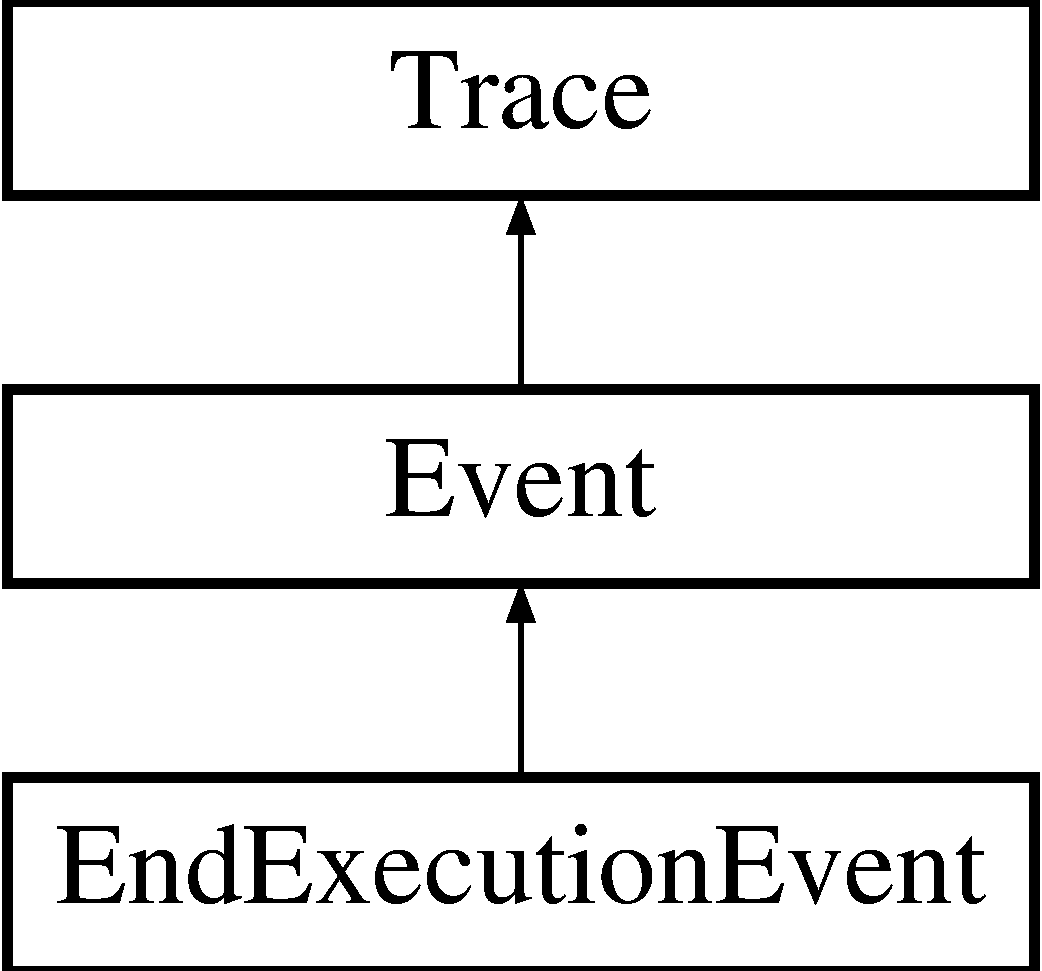
\includegraphics[height=3.000000cm]{class_end_execution_event}
\end{center}
\end{figure}
\subsection*{Public Member Functions}
\begin{DoxyCompactItemize}
\item 
\hyperlink{class_end_execution_event_a335a6695120ff70522e6b8ede3981fe9}{End\+Execution\+Event} (int end\+\_\+time)
\item 
\hyperlink{class_end_execution_event_aee725cbd3b770e439983e0174e8466ad}{End\+Execution\+Event} (const \hyperlink{class_end_execution_event}{End\+Execution\+Event} $\ast$eee)
\item 
virtual \hyperlink{class_trace_a9c58e523529fc8a03fb6acf3eef86150}{Trace\+::sp\+\_\+trace} \hyperlink{class_end_execution_event_aa89f0e0da951077ac408345235b7444b}{clone} () const 
\begin{DoxyCompactList}\small\item\em Clonage d\textquotesingle{}un événement. \end{DoxyCompactList}\item 
virtual std\+::string \hyperlink{class_end_execution_event_a8676ace3828d6b5914d76e90ec9a7105}{get\+Params} () const 
\begin{DoxyCompactList}\small\item\em Retourne les différents paramètres relatifs à l\textquotesingle{}événement sous forme de chaîne de caractères. \end{DoxyCompactList}\item 
int \hyperlink{class_end_execution_event_ae3642d03e060c6379a5149f9aef6d810}{get\+End\+Time} () const 
\end{DoxyCompactItemize}
\subsection*{Additional Inherited Members}


\subsection{Detailed Description}


Definition at line 109 of file Event\+Def.\+h.



\subsection{Constructor \& Destructor Documentation}
\index{End\+Execution\+Event@{End\+Execution\+Event}!End\+Execution\+Event@{End\+Execution\+Event}}
\index{End\+Execution\+Event@{End\+Execution\+Event}!End\+Execution\+Event@{End\+Execution\+Event}}
\subsubsection[{\texorpdfstring{End\+Execution\+Event(int end\+\_\+time)}{EndExecutionEvent(int end_time)}}]{\setlength{\rightskip}{0pt plus 5cm}End\+Execution\+Event\+::\+End\+Execution\+Event (
\begin{DoxyParamCaption}
\item[{int}]{end\+\_\+time}
\end{DoxyParamCaption}
)\hspace{0.3cm}{\ttfamily [inline]}}\hypertarget{class_end_execution_event_a335a6695120ff70522e6b8ede3981fe9}{}\label{class_end_execution_event_a335a6695120ff70522e6b8ede3981fe9}


Definition at line 113 of file Event\+Def.\+h.

\index{End\+Execution\+Event@{End\+Execution\+Event}!End\+Execution\+Event@{End\+Execution\+Event}}
\index{End\+Execution\+Event@{End\+Execution\+Event}!End\+Execution\+Event@{End\+Execution\+Event}}
\subsubsection[{\texorpdfstring{End\+Execution\+Event(const End\+Execution\+Event $\ast$eee)}{EndExecutionEvent(const EndExecutionEvent *eee)}}]{\setlength{\rightskip}{0pt plus 5cm}End\+Execution\+Event\+::\+End\+Execution\+Event (
\begin{DoxyParamCaption}
\item[{const {\bf End\+Execution\+Event} $\ast$}]{eee}
\end{DoxyParamCaption}
)\hspace{0.3cm}{\ttfamily [inline]}}\hypertarget{class_end_execution_event_aee725cbd3b770e439983e0174e8466ad}{}\label{class_end_execution_event_aee725cbd3b770e439983e0174e8466ad}


Definition at line 115 of file Event\+Def.\+h.



\subsection{Member Function Documentation}
\index{End\+Execution\+Event@{End\+Execution\+Event}!clone@{clone}}
\index{clone@{clone}!End\+Execution\+Event@{End\+Execution\+Event}}
\subsubsection[{\texorpdfstring{clone() const }{clone() const }}]{\setlength{\rightskip}{0pt plus 5cm}virtual {\bf Trace\+::sp\+\_\+trace} End\+Execution\+Event\+::clone (
\begin{DoxyParamCaption}
{}
\end{DoxyParamCaption}
) const\hspace{0.3cm}{\ttfamily [inline]}, {\ttfamily [virtual]}}\hypertarget{class_end_execution_event_aa89f0e0da951077ac408345235b7444b}{}\label{class_end_execution_event_aa89f0e0da951077ac408345235b7444b}


Clonage d\textquotesingle{}un événement. 

\begin{DoxyReturn}{Returns}
une copie de l\textquotesingle{}objet \hyperlink{class_event}{Event}. 
\end{DoxyReturn}


Reimplemented from \hyperlink{class_event_aafa2022d6600717a9cd6511797548265}{Event}.



Definition at line 119 of file Event\+Def.\+h.

\index{End\+Execution\+Event@{End\+Execution\+Event}!get\+End\+Time@{get\+End\+Time}}
\index{get\+End\+Time@{get\+End\+Time}!End\+Execution\+Event@{End\+Execution\+Event}}
\subsubsection[{\texorpdfstring{get\+End\+Time() const }{getEndTime() const }}]{\setlength{\rightskip}{0pt plus 5cm}int End\+Execution\+Event\+::get\+End\+Time (
\begin{DoxyParamCaption}
{}
\end{DoxyParamCaption}
) const\hspace{0.3cm}{\ttfamily [inline]}}\hypertarget{class_end_execution_event_ae3642d03e060c6379a5149f9aef6d810}{}\label{class_end_execution_event_ae3642d03e060c6379a5149f9aef6d810}


Definition at line 127 of file Event\+Def.\+h.

\index{End\+Execution\+Event@{End\+Execution\+Event}!get\+Params@{get\+Params}}
\index{get\+Params@{get\+Params}!End\+Execution\+Event@{End\+Execution\+Event}}
\subsubsection[{\texorpdfstring{get\+Params() const }{getParams() const }}]{\setlength{\rightskip}{0pt plus 5cm}virtual std\+::string End\+Execution\+Event\+::get\+Params (
\begin{DoxyParamCaption}
{}
\end{DoxyParamCaption}
) const\hspace{0.3cm}{\ttfamily [inline]}, {\ttfamily [virtual]}}\hypertarget{class_end_execution_event_a8676ace3828d6b5914d76e90ec9a7105}{}\label{class_end_execution_event_a8676ace3828d6b5914d76e90ec9a7105}


Retourne les différents paramètres relatifs à l\textquotesingle{}événement sous forme de chaîne de caractères. 

Cette fonction doit être redéfinie par les classes héritant de \hyperlink{class_event}{Event}.

\begin{DoxyReturn}{Returns}
la chaîne de caractères formatée contenant les valeurs des différents paramètres de l\textquotesingle{}événement séparées par des espaces. 
\end{DoxyReturn}


Reimplemented from \hyperlink{class_event_aad213c94070547bb727ba369b3460e2a}{Event}.



Definition at line 123 of file Event\+Def.\+h.



The documentation for this class was generated from the following file\+:\begin{DoxyCompactItemize}
\item 
C\+:/\+Users/\+Stephane/\+Desktop/mocahteam/\+Prog\+And\+Play/pp/traces/src/\hyperlink{_event_def_8h}{Event\+Def.\+h}\end{DoxyCompactItemize}

\hypertarget{class_end_mission_event}{}\section{End\+Mission\+Event Class Reference}
\label{class_end_mission_event}\index{End\+Mission\+Event@{End\+Mission\+Event}}


{\ttfamily \#include $<$Event\+Def.\+h$>$}

Inheritance diagram for End\+Mission\+Event\+:\begin{figure}[H]
\begin{center}
\leavevmode
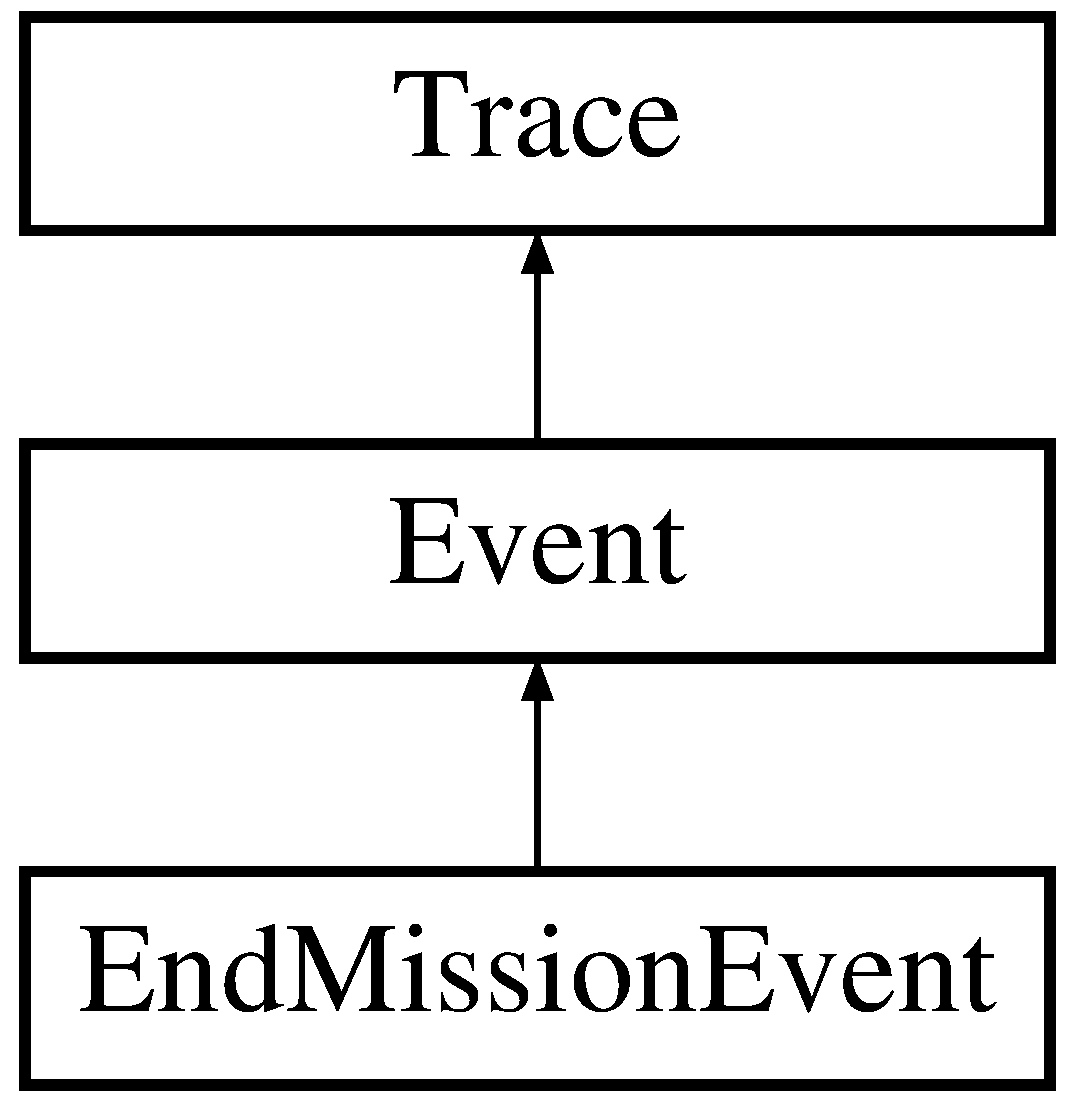
\includegraphics[height=3.000000cm]{class_end_mission_event}
\end{center}
\end{figure}
\subsection*{Public Member Functions}
\begin{DoxyCompactItemize}
\item 
\hyperlink{class_end_mission_event_af5771a5c2a68a7a892ac41adc1ba5ac0}{End\+Mission\+Event} (std\+::string status, int end\+\_\+time)
\item 
\hyperlink{class_end_mission_event_a14c57adacbdfd9b88bad741648ed6504}{End\+Mission\+Event} (const \hyperlink{class_end_mission_event}{End\+Mission\+Event} $\ast$eme)
\item 
virtual \hyperlink{class_trace_a9c58e523529fc8a03fb6acf3eef86150}{Trace\+::sp\+\_\+trace} \hyperlink{class_end_mission_event_a2d851feeb940eb1c73ab05d8cff28d84}{clone} () const 
\begin{DoxyCompactList}\small\item\em Clonage d\textquotesingle{}un événement. \end{DoxyCompactList}\item 
virtual std\+::string \hyperlink{class_end_mission_event_a79a3dc9a0bc4e39b4f9af2d1633a5029}{get\+Params} () const 
\begin{DoxyCompactList}\small\item\em Retourne les différents paramètres relatifs à l\textquotesingle{}événement sous forme de chaîne de caractères. \end{DoxyCompactList}\item 
std\+::string \hyperlink{class_end_mission_event_a8c67c8a4e0d03a4762ea08e85e40836a}{get\+Status} () const 
\item 
int \hyperlink{class_end_mission_event_a3336c51fe092b6d9740a9c20e73c45cb}{get\+End\+Time} () const 
\end{DoxyCompactItemize}
\subsection*{Additional Inherited Members}


\subsection{Detailed Description}


Definition at line 47 of file Event\+Def.\+h.



\subsection{Constructor \& Destructor Documentation}
\index{End\+Mission\+Event@{End\+Mission\+Event}!End\+Mission\+Event@{End\+Mission\+Event}}
\index{End\+Mission\+Event@{End\+Mission\+Event}!End\+Mission\+Event@{End\+Mission\+Event}}
\subsubsection[{\texorpdfstring{End\+Mission\+Event(std\+::string status, int end\+\_\+time)}{EndMissionEvent(std::string status, int end_time)}}]{\setlength{\rightskip}{0pt plus 5cm}End\+Mission\+Event\+::\+End\+Mission\+Event (
\begin{DoxyParamCaption}
\item[{std\+::string}]{status, }
\item[{int}]{end\+\_\+time}
\end{DoxyParamCaption}
)\hspace{0.3cm}{\ttfamily [inline]}}\hypertarget{class_end_mission_event_af5771a5c2a68a7a892ac41adc1ba5ac0}{}\label{class_end_mission_event_af5771a5c2a68a7a892ac41adc1ba5ac0}


Definition at line 51 of file Event\+Def.\+h.

\index{End\+Mission\+Event@{End\+Mission\+Event}!End\+Mission\+Event@{End\+Mission\+Event}}
\index{End\+Mission\+Event@{End\+Mission\+Event}!End\+Mission\+Event@{End\+Mission\+Event}}
\subsubsection[{\texorpdfstring{End\+Mission\+Event(const End\+Mission\+Event $\ast$eme)}{EndMissionEvent(const EndMissionEvent *eme)}}]{\setlength{\rightskip}{0pt plus 5cm}End\+Mission\+Event\+::\+End\+Mission\+Event (
\begin{DoxyParamCaption}
\item[{const {\bf End\+Mission\+Event} $\ast$}]{eme}
\end{DoxyParamCaption}
)\hspace{0.3cm}{\ttfamily [inline]}}\hypertarget{class_end_mission_event_a14c57adacbdfd9b88bad741648ed6504}{}\label{class_end_mission_event_a14c57adacbdfd9b88bad741648ed6504}


Definition at line 53 of file Event\+Def.\+h.



\subsection{Member Function Documentation}
\index{End\+Mission\+Event@{End\+Mission\+Event}!clone@{clone}}
\index{clone@{clone}!End\+Mission\+Event@{End\+Mission\+Event}}
\subsubsection[{\texorpdfstring{clone() const }{clone() const }}]{\setlength{\rightskip}{0pt plus 5cm}virtual {\bf Trace\+::sp\+\_\+trace} End\+Mission\+Event\+::clone (
\begin{DoxyParamCaption}
{}
\end{DoxyParamCaption}
) const\hspace{0.3cm}{\ttfamily [inline]}, {\ttfamily [virtual]}}\hypertarget{class_end_mission_event_a2d851feeb940eb1c73ab05d8cff28d84}{}\label{class_end_mission_event_a2d851feeb940eb1c73ab05d8cff28d84}


Clonage d\textquotesingle{}un événement. 

\begin{DoxyReturn}{Returns}
une copie de l\textquotesingle{}objet \hyperlink{class_event}{Event}. 
\end{DoxyReturn}


Reimplemented from \hyperlink{class_event_aafa2022d6600717a9cd6511797548265}{Event}.



Definition at line 58 of file Event\+Def.\+h.

\index{End\+Mission\+Event@{End\+Mission\+Event}!get\+End\+Time@{get\+End\+Time}}
\index{get\+End\+Time@{get\+End\+Time}!End\+Mission\+Event@{End\+Mission\+Event}}
\subsubsection[{\texorpdfstring{get\+End\+Time() const }{getEndTime() const }}]{\setlength{\rightskip}{0pt plus 5cm}int End\+Mission\+Event\+::get\+End\+Time (
\begin{DoxyParamCaption}
{}
\end{DoxyParamCaption}
) const\hspace{0.3cm}{\ttfamily [inline]}}\hypertarget{class_end_mission_event_a3336c51fe092b6d9740a9c20e73c45cb}{}\label{class_end_mission_event_a3336c51fe092b6d9740a9c20e73c45cb}


Definition at line 70 of file Event\+Def.\+h.

\index{End\+Mission\+Event@{End\+Mission\+Event}!get\+Params@{get\+Params}}
\index{get\+Params@{get\+Params}!End\+Mission\+Event@{End\+Mission\+Event}}
\subsubsection[{\texorpdfstring{get\+Params() const }{getParams() const }}]{\setlength{\rightskip}{0pt plus 5cm}virtual std\+::string End\+Mission\+Event\+::get\+Params (
\begin{DoxyParamCaption}
{}
\end{DoxyParamCaption}
) const\hspace{0.3cm}{\ttfamily [inline]}, {\ttfamily [virtual]}}\hypertarget{class_end_mission_event_a79a3dc9a0bc4e39b4f9af2d1633a5029}{}\label{class_end_mission_event_a79a3dc9a0bc4e39b4f9af2d1633a5029}


Retourne les différents paramètres relatifs à l\textquotesingle{}événement sous forme de chaîne de caractères. 

Cette fonction doit être redéfinie par les classes héritant de \hyperlink{class_event}{Event}.

\begin{DoxyReturn}{Returns}
la chaîne de caractères formatée contenant les valeurs des différents paramètres de l\textquotesingle{}événement séparées par des espaces. 
\end{DoxyReturn}


Reimplemented from \hyperlink{class_event_aad213c94070547bb727ba369b3460e2a}{Event}.



Definition at line 62 of file Event\+Def.\+h.

\index{End\+Mission\+Event@{End\+Mission\+Event}!get\+Status@{get\+Status}}
\index{get\+Status@{get\+Status}!End\+Mission\+Event@{End\+Mission\+Event}}
\subsubsection[{\texorpdfstring{get\+Status() const }{getStatus() const }}]{\setlength{\rightskip}{0pt plus 5cm}std\+::string End\+Mission\+Event\+::get\+Status (
\begin{DoxyParamCaption}
{}
\end{DoxyParamCaption}
) const\hspace{0.3cm}{\ttfamily [inline]}}\hypertarget{class_end_mission_event_a8c67c8a4e0d03a4762ea08e85e40836a}{}\label{class_end_mission_event_a8c67c8a4e0d03a4762ea08e85e40836a}


Definition at line 66 of file Event\+Def.\+h.



The documentation for this class was generated from the following file\+:\begin{DoxyCompactItemize}
\item 
C\+:/\+Users/\+Stephane/\+Desktop/mocahteam/\+Prog\+And\+Play/pp/traces/src/\hyperlink{_event_def_8h}{Event\+Def.\+h}\end{DoxyCompactItemize}

\hypertarget{class_event}{}\section{Event Class Reference}
\label{class_event}\index{Event@{Event}}


Classe héritant de \hyperlink{class_trace}{Trace}. Cette classe sert de classe mère pour toutes les classes définies dans le fichier \hyperlink{_event_def_8h}{Event\+Def.\+h}.  




{\ttfamily \#include $<$Event.\+h$>$}

Inheritance diagram for Event\+:\begin{figure}[H]
\begin{center}
\leavevmode
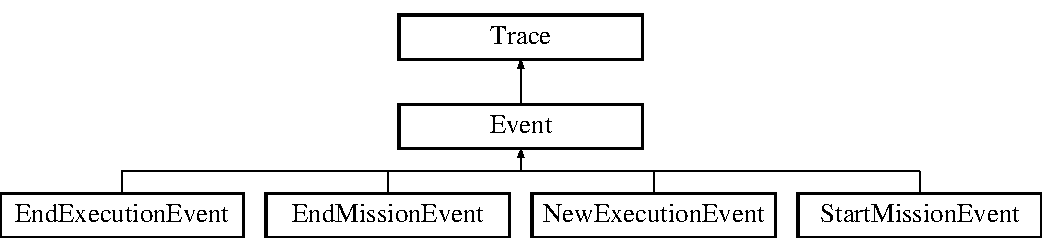
\includegraphics[height=3.000000cm]{class_event}
\end{center}
\end{figure}
\subsection*{Public Types}
\begin{DoxyCompactItemize}
\item 
typedef boost\+::shared\+\_\+ptr$<$ \hyperlink{class_event}{Event} $>$ \hyperlink{class_event_af09ed5d4baca5790d6decf72075dfe13}{sp\+\_\+event}
\end{DoxyCompactItemize}
\subsection*{Public Member Functions}
\begin{DoxyCompactItemize}
\item 
\hyperlink{class_event_a0effe34c8d7cf236f831b6a038ca5d94}{Event} (std\+::string \hyperlink{class_event_a8d9ecffd91cc944bee314f83260713ff}{label}, std\+::string \hyperlink{class_trace_a4835dcfa7da5d4c971e8f7d6860acb09}{info}=\char`\"{}\char`\"{})
\item 
\hyperlink{class_event_af490e691699bb4c74235fc9b224addee}{Event} (const \hyperlink{class_event}{Event} $\ast$e)
\item 
virtual unsigned int \hyperlink{class_event_adc33626b18f2090fba9f58cf0991fdb5}{length} () const 
\begin{DoxyCompactList}\small\item\em Récupération de la longueur (l\textquotesingle{}espace occupé dans un vecteur de traces) d\textquotesingle{}un événement. \end{DoxyCompactList}\item 
virtual bool \hyperlink{class_event_a33edb6d4cfa0dc8040a8a7e9e3e326d9}{operator==} (\hyperlink{class_trace}{Trace} $\ast$t) const 
\begin{DoxyCompactList}\small\item\em Comparaison de l\textquotesingle{}objet \hyperlink{class_event}{Event} avec une trace {\ttfamily t}. \end{DoxyCompactList}\item 
virtual \hyperlink{class_trace_a9c58e523529fc8a03fb6acf3eef86150}{Trace\+::sp\+\_\+trace} \hyperlink{class_event_aafa2022d6600717a9cd6511797548265}{clone} () const 
\begin{DoxyCompactList}\small\item\em Clonage d\textquotesingle{}un événement. \end{DoxyCompactList}\item 
virtual void \hyperlink{class_event_ae5465424aa2d50e2e144eae1d84a7ea9}{display} (std\+::ostream \&os=std\+::cout) const 
\begin{DoxyCompactList}\small\item\em Affichage des informations de l\textquotesingle{}objet \hyperlink{class_event}{Event}. \end{DoxyCompactList}\item 
virtual std\+::string \hyperlink{class_event_aad213c94070547bb727ba369b3460e2a}{get\+Params} () const 
\begin{DoxyCompactList}\small\item\em Retourne les différents paramètres relatifs à l\textquotesingle{}événement sous forme de chaîne de caractères. \end{DoxyCompactList}\item 
std\+::string \hyperlink{class_event_aadab1c703ff3bd4983da917badbb83d4}{get\+Label} () const 
\begin{DoxyCompactList}\small\item\em Getter pour la variable {\ttfamily label}. \end{DoxyCompactList}\end{DoxyCompactItemize}
\subsection*{Static Public Attributes}
\begin{DoxyCompactItemize}
\item 
static const char $\ast$ \hyperlink{class_event_a27d769cc30bbd8d827124958a9a95cae}{concat\+Events\+Arr} \mbox{[}$\,$\mbox{]} = \{\char`\"{}game\+\_\+paused\char`\"{}, \char`\"{}game\+\_\+unpaused\char`\"{}, N\+U\+LL\}
\item 
static const char $\ast$ \hyperlink{class_event_aaf275d46129b6cda2a84b905550349f2}{no\+Concat\+Events\+Arr} \mbox{[}$\,$\mbox{]} = \{\char`\"{}start\+\_\+mission\char`\"{}, \char`\"{}end\+\_\+mission\char`\"{}, \char`\"{}new\+\_\+execution\char`\"{}, \char`\"{}end\+\_\+execution\char`\"{}, \char`\"{}eof\char`\"{}, N\+U\+LL\}
\end{DoxyCompactItemize}
\subsection*{Protected Attributes}
\begin{DoxyCompactItemize}
\item 
std\+::string \hyperlink{class_event_a8d9ecffd91cc944bee314f83260713ff}{label}
\end{DoxyCompactItemize}
\subsection*{Additional Inherited Members}


\subsection{Detailed Description}
Classe héritant de \hyperlink{class_trace}{Trace}. Cette classe sert de classe mère pour toutes les classes définies dans le fichier \hyperlink{_event_def_8h}{Event\+Def.\+h}. 

Definition at line 19 of file Event.\+h.



\subsection{Member Typedef Documentation}
\index{Event@{Event}!sp\+\_\+event@{sp\+\_\+event}}
\index{sp\+\_\+event@{sp\+\_\+event}!Event@{Event}}
\subsubsection[{\texorpdfstring{sp\+\_\+event}{sp_event}}]{\setlength{\rightskip}{0pt plus 5cm}typedef boost\+::shared\+\_\+ptr$<${\bf Event}$>$ {\bf Event\+::sp\+\_\+event}}\hypertarget{class_event_af09ed5d4baca5790d6decf72075dfe13}{}\label{class_event_af09ed5d4baca5790d6decf72075dfe13}
Définition du type pointeur intelligent vers un objet \hyperlink{class_event}{Event}. 

Definition at line 26 of file Event.\+h.



\subsection{Constructor \& Destructor Documentation}
\index{Event@{Event}!Event@{Event}}
\index{Event@{Event}!Event@{Event}}
\subsubsection[{\texorpdfstring{Event(std\+::string label, std\+::string info="""")}{Event(std::string label, std::string info="")}}]{\setlength{\rightskip}{0pt plus 5cm}Event\+::\+Event (
\begin{DoxyParamCaption}
\item[{std\+::string}]{label, }
\item[{std\+::string}]{info = {\ttfamily \char`\"{}\char`\"{}}}
\end{DoxyParamCaption}
)}\hypertarget{class_event_a0effe34c8d7cf236f831b6a038ca5d94}{}\label{class_event_a0effe34c8d7cf236f831b6a038ca5d94}
Constructeur principal de la classe \hyperlink{class_event}{Event}.


\begin{DoxyParams}{Parameters}
{\em label} & le label de l\textquotesingle{}événement modélisé par l\textquotesingle{}objet \hyperlink{class_event}{Event}. \\
\hline
{\em info} & le label attribué par l\textquotesingle{}expert. \\
\hline
\end{DoxyParams}


Definition at line 6 of file Event.\+cpp.

\index{Event@{Event}!Event@{Event}}
\index{Event@{Event}!Event@{Event}}
\subsubsection[{\texorpdfstring{Event(const Event $\ast$e)}{Event(const Event *e)}}]{\setlength{\rightskip}{0pt plus 5cm}Event\+::\+Event (
\begin{DoxyParamCaption}
\item[{const {\bf Event} $\ast$}]{e}
\end{DoxyParamCaption}
)}\hypertarget{class_event_af490e691699bb4c74235fc9b224addee}{}\label{class_event_af490e691699bb4c74235fc9b224addee}
Constructeur de la classe \hyperlink{class_event}{Event} utilisé notamment lors de la copie de l\textquotesingle{}objet. 

Definition at line 8 of file Event.\+cpp.



\subsection{Member Function Documentation}
\index{Event@{Event}!clone@{clone}}
\index{clone@{clone}!Event@{Event}}
\subsubsection[{\texorpdfstring{clone() const }{clone() const }}]{\setlength{\rightskip}{0pt plus 5cm}{\bf Trace\+::sp\+\_\+trace} Event\+::clone (
\begin{DoxyParamCaption}
{}
\end{DoxyParamCaption}
) const\hspace{0.3cm}{\ttfamily [virtual]}}\hypertarget{class_event_aafa2022d6600717a9cd6511797548265}{}\label{class_event_aafa2022d6600717a9cd6511797548265}


Clonage d\textquotesingle{}un événement. 

\begin{DoxyReturn}{Returns}
une copie de l\textquotesingle{}objet \hyperlink{class_event}{Event}. 
\end{DoxyReturn}


Implements \hyperlink{class_trace_a0917758337e37f936713ccaf75b532f2}{Trace}.



Reimplemented in \hyperlink{class_end_execution_event_aa89f0e0da951077ac408345235b7444b}{End\+Execution\+Event}, \hyperlink{class_new_execution_event_adc75351c4c45e5161c26138b29e980ed}{New\+Execution\+Event}, \hyperlink{class_end_mission_event_a2d851feeb940eb1c73ab05d8cff28d84}{End\+Mission\+Event}, and \hyperlink{class_start_mission_event_a4dcda1cb85c391e3594ab1486bc3223d}{Start\+Mission\+Event}.



Definition at line 22 of file Event.\+cpp.

\index{Event@{Event}!display@{display}}
\index{display@{display}!Event@{Event}}
\subsubsection[{\texorpdfstring{display(std\+::ostream \&os=std\+::cout) const }{display(std::ostream &os=std::cout) const }}]{\setlength{\rightskip}{0pt plus 5cm}void Event\+::display (
\begin{DoxyParamCaption}
\item[{std\+::ostream \&}]{os = {\ttfamily std\+:\+:cout}}
\end{DoxyParamCaption}
) const\hspace{0.3cm}{\ttfamily [virtual]}}\hypertarget{class_event_ae5465424aa2d50e2e144eae1d84a7ea9}{}\label{class_event_ae5465424aa2d50e2e144eae1d84a7ea9}


Affichage des informations de l\textquotesingle{}objet \hyperlink{class_event}{Event}. 


\begin{DoxyParams}{Parameters}
{\em os} & le flux de sortie utilisé pour l\textquotesingle{}affichage. \\
\hline
\end{DoxyParams}


Implements \hyperlink{class_trace_a4324fa45af235238ddedc2215c3d1cf0}{Trace}.



Definition at line 26 of file Event.\+cpp.

\index{Event@{Event}!get\+Label@{get\+Label}}
\index{get\+Label@{get\+Label}!Event@{Event}}
\subsubsection[{\texorpdfstring{get\+Label() const }{getLabel() const }}]{\setlength{\rightskip}{0pt plus 5cm}std\+::string Event\+::get\+Label (
\begin{DoxyParamCaption}
{}
\end{DoxyParamCaption}
) const}\hypertarget{class_event_aadab1c703ff3bd4983da917badbb83d4}{}\label{class_event_aadab1c703ff3bd4983da917badbb83d4}


Getter pour la variable {\ttfamily label}. 

\begin{DoxyReturn}{Returns}
la chaîne de caractères {\ttfamily label} associée à l\textquotesingle{}événement. 
\end{DoxyReturn}


Definition at line 37 of file Event.\+cpp.

\index{Event@{Event}!get\+Params@{get\+Params}}
\index{get\+Params@{get\+Params}!Event@{Event}}
\subsubsection[{\texorpdfstring{get\+Params() const }{getParams() const }}]{\setlength{\rightskip}{0pt plus 5cm}std\+::string Event\+::get\+Params (
\begin{DoxyParamCaption}
{}
\end{DoxyParamCaption}
) const\hspace{0.3cm}{\ttfamily [virtual]}}\hypertarget{class_event_aad213c94070547bb727ba369b3460e2a}{}\label{class_event_aad213c94070547bb727ba369b3460e2a}


Retourne les différents paramètres relatifs à l\textquotesingle{}événement sous forme de chaîne de caractères. 

Cette fonction doit être redéfinie par les classes héritant de \hyperlink{class_event}{Event}.

\begin{DoxyReturn}{Returns}
la chaîne de caractères formatée contenant les valeurs des différents paramètres de l\textquotesingle{}événement séparées par des espaces. 
\end{DoxyReturn}


Reimplemented in \hyperlink{class_end_execution_event_a8676ace3828d6b5914d76e90ec9a7105}{End\+Execution\+Event}, \hyperlink{class_new_execution_event_a1d28826bae4c7b73bc85859f62f48a48}{New\+Execution\+Event}, \hyperlink{class_end_mission_event_a79a3dc9a0bc4e39b4f9af2d1633a5029}{End\+Mission\+Event}, and \hyperlink{class_start_mission_event_a498a3b6e3fa6dfd736486aaa1db421dd}{Start\+Mission\+Event}.



Definition at line 41 of file Event.\+cpp.

\index{Event@{Event}!length@{length}}
\index{length@{length}!Event@{Event}}
\subsubsection[{\texorpdfstring{length() const }{length() const }}]{\setlength{\rightskip}{0pt plus 5cm}unsigned int Event\+::length (
\begin{DoxyParamCaption}
{}
\end{DoxyParamCaption}
) const\hspace{0.3cm}{\ttfamily [virtual]}}\hypertarget{class_event_adc33626b18f2090fba9f58cf0991fdb5}{}\label{class_event_adc33626b18f2090fba9f58cf0991fdb5}


Récupération de la longueur (l\textquotesingle{}espace occupé dans un vecteur de traces) d\textquotesingle{}un événement. 

\begin{DoxyReturn}{Returns}
0 
\end{DoxyReturn}


Implements \hyperlink{class_trace_a74a29f7e259781424d9f81409ed34701}{Trace}.



Definition at line 33 of file Event.\+cpp.

\index{Event@{Event}!operator==@{operator==}}
\index{operator==@{operator==}!Event@{Event}}
\subsubsection[{\texorpdfstring{operator==(\+Trace $\ast$t) const }{operator==(Trace *t) const }}]{\setlength{\rightskip}{0pt plus 5cm}bool Event\+::operator== (
\begin{DoxyParamCaption}
\item[{{\bf Trace} $\ast$}]{t}
\end{DoxyParamCaption}
) const\hspace{0.3cm}{\ttfamily [virtual]}}\hypertarget{class_event_a33edb6d4cfa0dc8040a8a7e9e3e326d9}{}\label{class_event_a33edb6d4cfa0dc8040a8a7e9e3e326d9}


Comparaison de l\textquotesingle{}objet \hyperlink{class_event}{Event} avec une trace {\ttfamily t}. 


\begin{DoxyParams}{Parameters}
{\em t} & \+: la trace utilisée pour la comparaison.\\
\hline
\end{DoxyParams}
\begin{DoxyReturn}{Returns}
vrai si la trace {\ttfamily t} est également un événement et si elle a le même label que cet événement. 
\end{DoxyReturn}


Implements \hyperlink{class_trace_a8201809c2fcc1d02cfa8bf894a79bb5e}{Trace}.



Definition at line 12 of file Event.\+cpp.



\subsection{Member Data Documentation}
\index{Event@{Event}!concat\+Events\+Arr@{concat\+Events\+Arr}}
\index{concat\+Events\+Arr@{concat\+Events\+Arr}!Event@{Event}}
\subsubsection[{\texorpdfstring{concat\+Events\+Arr}{concatEventsArr}}]{\setlength{\rightskip}{0pt plus 5cm}const char $\ast$ Event\+::concat\+Events\+Arr = \{\char`\"{}game\+\_\+paused\char`\"{}, \char`\"{}game\+\_\+unpaused\char`\"{}, N\+U\+LL\}\hspace{0.3cm}{\ttfamily [static]}}\hypertarget{class_event_a27d769cc30bbd8d827124958a9a95cae}{}\label{class_event_a27d769cc30bbd8d827124958a9a95cae}
Tableau contenant les labels des événements pris en compte lors du parsing du fichier de traces brutes.

\begin{DoxySeeAlso}{See also}
\hyperlink{class_traces_parser_af094e480d2d92e273ec454cc8bdb4c56}{Traces\+Parser\+::handle\+Line} 
\end{DoxySeeAlso}


Definition at line 46 of file Event.\+h.

\index{Event@{Event}!label@{label}}
\index{label@{label}!Event@{Event}}
\subsubsection[{\texorpdfstring{label}{label}}]{\setlength{\rightskip}{0pt plus 5cm}std\+::string Event\+::label\hspace{0.3cm}{\ttfamily [protected]}}\hypertarget{class_event_a8d9ecffd91cc944bee314f83260713ff}{}\label{class_event_a8d9ecffd91cc944bee314f83260713ff}
Le label associé permettant d\textquotesingle{}identifier l\textquotesingle{}événement modélisé par l\textquotesingle{}objet \hyperlink{class_event}{Event}. 

Definition at line 104 of file Event.\+h.

\index{Event@{Event}!no\+Concat\+Events\+Arr@{no\+Concat\+Events\+Arr}}
\index{no\+Concat\+Events\+Arr@{no\+Concat\+Events\+Arr}!Event@{Event}}
\subsubsection[{\texorpdfstring{no\+Concat\+Events\+Arr}{noConcatEventsArr}}]{\setlength{\rightskip}{0pt plus 5cm}const char $\ast$ Event\+::no\+Concat\+Events\+Arr = \{\char`\"{}start\+\_\+mission\char`\"{}, \char`\"{}end\+\_\+mission\char`\"{}, \char`\"{}new\+\_\+execution\char`\"{}, \char`\"{}end\+\_\+execution\char`\"{}, \char`\"{}eof\char`\"{}, N\+U\+LL\}\hspace{0.3cm}{\ttfamily [static]}}\hypertarget{class_event_aaf275d46129b6cda2a84b905550349f2}{}\label{class_event_aaf275d46129b6cda2a84b905550349f2}
Tableau contenant les labels des événements définissant les débuts/fins de mission/d\textquotesingle{}éxécution. 

Definition at line 51 of file Event.\+h.



The documentation for this class was generated from the following files\+:\begin{DoxyCompactItemize}
\item 
C\+:/\+Users/\+Stephane/\+Desktop/mocahteam/\+Prog\+And\+Play/pp/traces/src/\hyperlink{_event_8h}{Event.\+h}\item 
C\+:/\+Users/\+Stephane/\+Desktop/mocahteam/\+Prog\+And\+Play/pp/traces/src/\hyperlink{_event_8cpp}{Event.\+cpp}\end{DoxyCompactItemize}

\hypertarget{struct_traces_analyser_1_1_feedback}{}\section{Traces\+Analyser\+:\+:Feedback Struct Reference}
\label{struct_traces_analyser_1_1_feedback}\index{Traces\+Analyser\+::\+Feedback@{Traces\+Analyser\+::\+Feedback}}


{\ttfamily \#include $<$Traces\+Analyser.\+h$>$}

\subsection*{Public Member Functions}
\begin{DoxyCompactItemize}
\item 
bool \hyperlink{struct_traces_analyser_1_1_feedback_a3597de15c1c142a06bc044d35eff110a}{operator$<$} (const \hyperlink{struct_traces_analyser_1_1_feedback}{Feedback} \&f) const 
\begin{DoxyCompactList}\small\item\em Fonction utilisé lors de l\textquotesingle{}opération de tri des feedbacks listés. \end{DoxyCompactList}\item 
void \hyperlink{struct_traces_analyser_1_1_feedback_affc7db79662d3e99b01e3cf3ca5e1616}{display} (std\+::ostream \&os=std\+::cout)
\begin{DoxyCompactList}\small\item\em Affichage du feedback. \end{DoxyCompactList}\end{DoxyCompactItemize}
\subsection*{Public Attributes}
\begin{DoxyCompactItemize}
\item 
\hyperlink{class_traces_analyser_a57be29ce5ac10ca51e56d8385b4a1820}{Feedback\+Type} \hyperlink{struct_traces_analyser_1_1_feedback_a828dbdc4ca2e76874679e91a5245996e}{type}
\item 
std\+::string \hyperlink{struct_traces_analyser_1_1_feedback_a3300931839b28cbf4a2d1faa3028c679}{info}
\item 
\hyperlink{class_trace_a9c58e523529fc8a03fb6acf3eef86150}{Trace\+::sp\+\_\+trace} \hyperlink{struct_traces_analyser_1_1_feedback_a1c4848a6f5ad484386c1baaac8270a27}{learner\+\_\+spt}
\item 
\hyperlink{class_trace_a9c58e523529fc8a03fb6acf3eef86150}{Trace\+::sp\+\_\+trace} \hyperlink{struct_traces_analyser_1_1_feedback_ab0783087941c78c1ac592a1e284d4396}{expert\+\_\+spt}
\item 
int \hyperlink{struct_traces_analyser_1_1_feedback_ad139e027aaebcb9f3b4cfe4a5a7c5ff7}{priority}
\item 
int \hyperlink{struct_traces_analyser_1_1_feedback_a4ec88472bb7b925d548267cb263ee81b}{level}
\item 
bool \hyperlink{struct_traces_analyser_1_1_feedback_a3d84d2d22c4639d2c04789c054120c27}{defined}
\end{DoxyCompactItemize}


\subsection{Detailed Description}
Structure utilisée pour contenir un ensemble d\textquotesingle{}informations sur un retour qui pourrait être donné au joueur. 

Definition at line 175 of file Traces\+Analyser.\+h.



\subsection{Member Function Documentation}
\index{Traces\+Analyser\+::\+Feedback@{Traces\+Analyser\+::\+Feedback}!display@{display}}
\index{display@{display}!Traces\+Analyser\+::\+Feedback@{Traces\+Analyser\+::\+Feedback}}
\subsubsection[{\texorpdfstring{display(std\+::ostream \&os=std\+::cout)}{display(std::ostream &os=std::cout)}}]{\setlength{\rightskip}{0pt plus 5cm}void Traces\+Analyser\+::\+Feedback\+::display (
\begin{DoxyParamCaption}
\item[{std\+::ostream \&}]{os = {\ttfamily std\+:\+:cout}}
\end{DoxyParamCaption}
)\hspace{0.3cm}{\ttfamily [inline]}}\hypertarget{struct_traces_analyser_1_1_feedback_affc7db79662d3e99b01e3cf3ca5e1616}{}\label{struct_traces_analyser_1_1_feedback_affc7db79662d3e99b01e3cf3ca5e1616}


Affichage du feedback. 


\begin{DoxyParams}{Parameters}
{\em os} & le flux de sortie utilisé pour l\textquotesingle{}affichage. \\
\hline
\end{DoxyParams}


Definition at line 231 of file Traces\+Analyser.\+h.

\index{Traces\+Analyser\+::\+Feedback@{Traces\+Analyser\+::\+Feedback}!operator$<$@{operator$<$}}
\index{operator$<$@{operator$<$}!Traces\+Analyser\+::\+Feedback@{Traces\+Analyser\+::\+Feedback}}
\subsubsection[{\texorpdfstring{operator$<$(const Feedback \&f) const }{operator<(const Feedback &f) const }}]{\setlength{\rightskip}{0pt plus 5cm}bool Traces\+Analyser\+::\+Feedback\+::operator$<$ (
\begin{DoxyParamCaption}
\item[{const {\bf Feedback} \&}]{f}
\end{DoxyParamCaption}
) const\hspace{0.3cm}{\ttfamily [inline]}}\hypertarget{struct_traces_analyser_1_1_feedback_a3597de15c1c142a06bc044d35eff110a}{}\label{struct_traces_analyser_1_1_feedback_a3597de15c1c142a06bc044d35eff110a}


Fonction utilisé lors de l\textquotesingle{}opération de tri des feedbacks listés. 


\begin{DoxyParams}{Parameters}
{\em f} & l\textquotesingle{}objet \hyperlink{struct_traces_analyser_1_1_feedback}{Feedback} utilisé pour la comparaison. \\
\hline
\end{DoxyParams}


Definition at line 221 of file Traces\+Analyser.\+h.



\subsection{Member Data Documentation}
\index{Traces\+Analyser\+::\+Feedback@{Traces\+Analyser\+::\+Feedback}!defined@{defined}}
\index{defined@{defined}!Traces\+Analyser\+::\+Feedback@{Traces\+Analyser\+::\+Feedback}}
\subsubsection[{\texorpdfstring{defined}{defined}}]{\setlength{\rightskip}{0pt plus 5cm}bool Traces\+Analyser\+::\+Feedback\+::defined}\hypertarget{struct_traces_analyser_1_1_feedback_a3d84d2d22c4639d2c04789c054120c27}{}\label{struct_traces_analyser_1_1_feedback_a3d84d2d22c4639d2c04789c054120c27}
Booléen mis à vrai si un pattern a été défini pour le feedback dans le fichier X\+ML de définition de feedbacks, i.\+e. si learner\+\_\+spt OU (non exclusif) expert\+\_\+spt est défini. 

Definition at line 213 of file Traces\+Analyser.\+h.

\index{Traces\+Analyser\+::\+Feedback@{Traces\+Analyser\+::\+Feedback}!expert\+\_\+spt@{expert\+\_\+spt}}
\index{expert\+\_\+spt@{expert\+\_\+spt}!Traces\+Analyser\+::\+Feedback@{Traces\+Analyser\+::\+Feedback}}
\subsubsection[{\texorpdfstring{expert\+\_\+spt}{expert_spt}}]{\setlength{\rightskip}{0pt plus 5cm}{\bf Trace\+::sp\+\_\+trace} Traces\+Analyser\+::\+Feedback\+::expert\+\_\+spt}\hypertarget{struct_traces_analyser_1_1_feedback_ab0783087941c78c1ac592a1e284d4396}{}\label{struct_traces_analyser_1_1_feedback_ab0783087941c78c1ac592a1e284d4396}
\hyperlink{class_trace}{Trace} de l\textquotesingle{}expert défini pour ce feedback. Défini par la balise $<$expert$>$ dans un fichier X\+ML de définition de feedbacks. 

Definition at line 198 of file Traces\+Analyser.\+h.

\index{Traces\+Analyser\+::\+Feedback@{Traces\+Analyser\+::\+Feedback}!info@{info}}
\index{info@{info}!Traces\+Analyser\+::\+Feedback@{Traces\+Analyser\+::\+Feedback}}
\subsubsection[{\texorpdfstring{info}{info}}]{\setlength{\rightskip}{0pt plus 5cm}std\+::string Traces\+Analyser\+::\+Feedback\+::info}\hypertarget{struct_traces_analyser_1_1_feedback_a3300931839b28cbf4a2d1faa3028c679}{}\label{struct_traces_analyser_1_1_feedback_a3300931839b28cbf4a2d1faa3028c679}
Chaîne de caractères contenant le texte associé au feedback. Défini par la balise $<$info$>$ dans un fichier X\+ML de définition de feedbacks. A noter que la balise $<$infos lang=\char`\"{}...\char`\"{}$>$ doit contenir au moins une balise $<$info$>$ pour la langue choisie. 

Definition at line 188 of file Traces\+Analyser.\+h.

\index{Traces\+Analyser\+::\+Feedback@{Traces\+Analyser\+::\+Feedback}!learner\+\_\+spt@{learner\+\_\+spt}}
\index{learner\+\_\+spt@{learner\+\_\+spt}!Traces\+Analyser\+::\+Feedback@{Traces\+Analyser\+::\+Feedback}}
\subsubsection[{\texorpdfstring{learner\+\_\+spt}{learner_spt}}]{\setlength{\rightskip}{0pt plus 5cm}{\bf Trace\+::sp\+\_\+trace} Traces\+Analyser\+::\+Feedback\+::learner\+\_\+spt}\hypertarget{struct_traces_analyser_1_1_feedback_a1c4848a6f5ad484386c1baaac8270a27}{}\label{struct_traces_analyser_1_1_feedback_a1c4848a6f5ad484386c1baaac8270a27}
\hyperlink{class_trace}{Trace} de l\textquotesingle{}apprenant pour ce feedback. Défini par la balise $<$learner$>$ dans un fichier X\+ML de définition de feedbacks. 

Definition at line 193 of file Traces\+Analyser.\+h.

\index{Traces\+Analyser\+::\+Feedback@{Traces\+Analyser\+::\+Feedback}!level@{level}}
\index{level@{level}!Traces\+Analyser\+::\+Feedback@{Traces\+Analyser\+::\+Feedback}}
\subsubsection[{\texorpdfstring{level}{level}}]{\setlength{\rightskip}{0pt plus 5cm}int Traces\+Analyser\+::\+Feedback\+::level}\hypertarget{struct_traces_analyser_1_1_feedback_a4ec88472bb7b925d548267cb263ee81b}{}\label{struct_traces_analyser_1_1_feedback_a4ec88472bb7b925d548267cb263ee81b}
Variable prenant la valeur de l\textquotesingle{}attribut \textquotesingle{}level\textquotesingle{} associé à la balise $<$feedback$>$ dans le fichier X\+ML de définition de feedbacks. Cet attribut est optionnel. S\textquotesingle{}il n\textquotesingle{}est pas défini, cette variable prend la valeur -\/1 et ne sera pas utilisée lors de l\textquotesingle{}analyse. Dans le cas, où il est défini, sa valeur est utilisée pour associer un niveau aux traces {\ttfamily learner\+\_\+spt} et {\ttfamily expert\+\_\+spt}. 

Definition at line 208 of file Traces\+Analyser.\+h.

\index{Traces\+Analyser\+::\+Feedback@{Traces\+Analyser\+::\+Feedback}!priority@{priority}}
\index{priority@{priority}!Traces\+Analyser\+::\+Feedback@{Traces\+Analyser\+::\+Feedback}}
\subsubsection[{\texorpdfstring{priority}{priority}}]{\setlength{\rightskip}{0pt plus 5cm}int Traces\+Analyser\+::\+Feedback\+::priority}\hypertarget{struct_traces_analyser_1_1_feedback_ad139e027aaebcb9f3b4cfe4a5a7c5ff7}{}\label{struct_traces_analyser_1_1_feedback_ad139e027aaebcb9f3b4cfe4a5a7c5ff7}
Priorité associée au feedback. Ce champ est obligatoire dans le fichier X\+ML de définition de feedbacks. 

Definition at line 203 of file Traces\+Analyser.\+h.

\index{Traces\+Analyser\+::\+Feedback@{Traces\+Analyser\+::\+Feedback}!type@{type}}
\index{type@{type}!Traces\+Analyser\+::\+Feedback@{Traces\+Analyser\+::\+Feedback}}
\subsubsection[{\texorpdfstring{type}{type}}]{\setlength{\rightskip}{0pt plus 5cm}{\bf Feedback\+Type} Traces\+Analyser\+::\+Feedback\+::type}\hypertarget{struct_traces_analyser_1_1_feedback_a828dbdc4ca2e76874679e91a5245996e}{}\label{struct_traces_analyser_1_1_feedback_a828dbdc4ca2e76874679e91a5245996e}
Définition du type du feedback. Ce champ est obligatoire dans le fichier X\+ML de définition de feedbacks.

\begin{DoxySeeAlso}{See also}
\hyperlink{class_traces_analyser_a57be29ce5ac10ca51e56d8385b4a1820}{Feedback\+Type} 
\end{DoxySeeAlso}


Definition at line 182 of file Traces\+Analyser.\+h.



The documentation for this struct was generated from the following file\+:\begin{DoxyCompactItemize}
\item 
C\+:/\+Users/\+Stephane/\+Desktop/mocahteam/\+Prog\+And\+Play/pp/traces/src/\hyperlink{_traces_analyser_8h}{Traces\+Analyser.\+h}\end{DoxyCompactItemize}

\hypertarget{struct_traces_analyser_1_1_game_infos}{}\section{Traces\+Analyser\+:\+:Game\+Infos Struct Reference}
\label{struct_traces_analyser_1_1_game_infos}\index{Traces\+Analyser\+::\+Game\+Infos@{Traces\+Analyser\+::\+Game\+Infos}}


{\ttfamily \#include $<$Traces\+Analyser.\+h$>$}

\subsection*{Public Member Functions}
\begin{DoxyCompactItemize}
\item 
\hyperlink{struct_traces_analyser_1_1_game_infos_a6c95d2699b29e297aaaaed93fca6446a}{Game\+Infos} ()
\begin{DoxyCompactList}\small\item\em Constructeur de \hyperlink{struct_traces_analyser_1_1_game_infos}{Game\+Infos}. \end{DoxyCompactList}\item 
void \hyperlink{struct_traces_analyser_1_1_game_infos_a313f36b89634c6cdcd68274f3fa7318d}{clear\+Mission} ()
\begin{DoxyCompactList}\small\item\em Réinitialise toutes les informations de l\textquotesingle{}objet \hyperlink{struct_traces_analyser_1_1_game_infos}{Game\+Infos}. \end{DoxyCompactList}\item 
void \hyperlink{struct_traces_analyser_1_1_game_infos_aee048954110f387b71d66ef5528c09d5}{clear\+Execution} ()
\begin{DoxyCompactList}\small\item\em Réinitialise toutes les informations relatives à une exécution. \end{DoxyCompactList}\item 
int \hyperlink{struct_traces_analyser_1_1_game_infos_a67c16e181087d3fceab87a4ac786a24a}{get\+Resolution\+Time} ()
\begin{DoxyCompactList}\small\item\em Calcul du temps de résolution de la mission. \end{DoxyCompactList}\item 
int \hyperlink{struct_traces_analyser_1_1_game_infos_a7736e87dac7d9caa86b8b27560f2e95f}{get\+Execution\+Time} ()
\begin{DoxyCompactList}\small\item\em Calcul du temps d\textquotesingle{}exécution du programme de résolution de la mission. \end{DoxyCompactList}\item 
int \hyperlink{struct_traces_analyser_1_1_game_infos_a41d562577af62e38a8c0b8d9aa9f9ce7}{get\+Num\+Executions} ()
\begin{DoxyCompactList}\small\item\em Calcul du nombre d\textquotesingle{}exécutions lancées par le joueur pour résoudre une mission. \end{DoxyCompactList}\item 
double \hyperlink{struct_traces_analyser_1_1_game_infos_abd4e2397d4f2fa5e290420ad9fe93019}{get\+Average\+Wait\+Time} ()
\begin{DoxyCompactList}\small\item\em Calcul du temps moyen d\textquotesingle{}attente entre deux exécutions. \end{DoxyCompactList}\end{DoxyCompactItemize}
\subsection*{Public Attributes}
\begin{DoxyCompactItemize}
\item 
\hyperlink{class_start_mission_event}{Start\+Mission\+Event} $\ast$ \hyperlink{struct_traces_analyser_1_1_game_infos_ae14dc2f1fb7fd6f6ebc774adcc7453ff}{sme}
\item 
\hyperlink{class_end_mission_event}{End\+Mission\+Event} $\ast$ \hyperlink{struct_traces_analyser_1_1_game_infos_a626886085d8342aaa0bb35d4ef768a2d}{eme}
\item 
\hyperlink{class_new_execution_event}{New\+Execution\+Event} $\ast$ \hyperlink{struct_traces_analyser_1_1_game_infos_a9536f8b96fa309397655264cc2983063}{nee}
\item 
\hyperlink{class_end_execution_event}{End\+Execution\+Event} $\ast$ \hyperlink{struct_traces_analyser_1_1_game_infos_ad8bab50191b3a7d55dbeb60b88e12de7}{eee}
\item 
std\+::vector$<$ \hyperlink{class_trace_a9c58e523529fc8a03fb6acf3eef86150}{Trace\+::sp\+\_\+trace} $>$ \hyperlink{struct_traces_analyser_1_1_game_infos_a97beef39c7cb8d643ba4f11de8b7073b}{mission\+\_\+traces}
\item 
\hyperlink{class_sequence_a796bfa70aa4ddd4e447c210655b5dc5a}{Sequence\+::sp\+\_\+sequence} \hyperlink{struct_traces_analyser_1_1_game_infos_a674838500aafddb2a17153413708be08}{root\+\_\+sps}
\end{DoxyCompactItemize}


\subsection{Detailed Description}
Structure utilisée pour contenir un ensemble d\textquotesingle{}informations sur une trace compressée. 

Definition at line 250 of file Traces\+Analyser.\+h.



\subsection{Constructor \& Destructor Documentation}
\index{Traces\+Analyser\+::\+Game\+Infos@{Traces\+Analyser\+::\+Game\+Infos}!Game\+Infos@{Game\+Infos}}
\index{Game\+Infos@{Game\+Infos}!Traces\+Analyser\+::\+Game\+Infos@{Traces\+Analyser\+::\+Game\+Infos}}
\subsubsection[{\texorpdfstring{Game\+Infos()}{GameInfos()}}]{\setlength{\rightskip}{0pt plus 5cm}Traces\+Analyser\+::\+Game\+Infos\+::\+Game\+Infos (
\begin{DoxyParamCaption}
{}
\end{DoxyParamCaption}
)\hspace{0.3cm}{\ttfamily [inline]}}\hypertarget{struct_traces_analyser_1_1_game_infos_a6c95d2699b29e297aaaaed93fca6446a}{}\label{struct_traces_analyser_1_1_game_infos_a6c95d2699b29e297aaaaed93fca6446a}


Constructeur de \hyperlink{struct_traces_analyser_1_1_game_infos}{Game\+Infos}. 



Definition at line 286 of file Traces\+Analyser.\+h.



\subsection{Member Function Documentation}
\index{Traces\+Analyser\+::\+Game\+Infos@{Traces\+Analyser\+::\+Game\+Infos}!clear\+Execution@{clear\+Execution}}
\index{clear\+Execution@{clear\+Execution}!Traces\+Analyser\+::\+Game\+Infos@{Traces\+Analyser\+::\+Game\+Infos}}
\subsubsection[{\texorpdfstring{clear\+Execution()}{clearExecution()}}]{\setlength{\rightskip}{0pt plus 5cm}void Traces\+Analyser\+::\+Game\+Infos\+::clear\+Execution (
\begin{DoxyParamCaption}
{}
\end{DoxyParamCaption}
)\hspace{0.3cm}{\ttfamily [inline]}}\hypertarget{struct_traces_analyser_1_1_game_infos_aee048954110f387b71d66ef5528c09d5}{}\label{struct_traces_analyser_1_1_game_infos_aee048954110f387b71d66ef5528c09d5}


Réinitialise toutes les informations relatives à une exécution. 



Definition at line 301 of file Traces\+Analyser.\+h.

\index{Traces\+Analyser\+::\+Game\+Infos@{Traces\+Analyser\+::\+Game\+Infos}!clear\+Mission@{clear\+Mission}}
\index{clear\+Mission@{clear\+Mission}!Traces\+Analyser\+::\+Game\+Infos@{Traces\+Analyser\+::\+Game\+Infos}}
\subsubsection[{\texorpdfstring{clear\+Mission()}{clearMission()}}]{\setlength{\rightskip}{0pt plus 5cm}void Traces\+Analyser\+::\+Game\+Infos\+::clear\+Mission (
\begin{DoxyParamCaption}
{}
\end{DoxyParamCaption}
)\hspace{0.3cm}{\ttfamily [inline]}}\hypertarget{struct_traces_analyser_1_1_game_infos_a313f36b89634c6cdcd68274f3fa7318d}{}\label{struct_traces_analyser_1_1_game_infos_a313f36b89634c6cdcd68274f3fa7318d}


Réinitialise toutes les informations de l\textquotesingle{}objet \hyperlink{struct_traces_analyser_1_1_game_infos}{Game\+Infos}. 



Definition at line 291 of file Traces\+Analyser.\+h.

\index{Traces\+Analyser\+::\+Game\+Infos@{Traces\+Analyser\+::\+Game\+Infos}!get\+Average\+Wait\+Time@{get\+Average\+Wait\+Time}}
\index{get\+Average\+Wait\+Time@{get\+Average\+Wait\+Time}!Traces\+Analyser\+::\+Game\+Infos@{Traces\+Analyser\+::\+Game\+Infos}}
\subsubsection[{\texorpdfstring{get\+Average\+Wait\+Time()}{getAverageWaitTime()}}]{\setlength{\rightskip}{0pt plus 5cm}double Traces\+Analyser\+::\+Game\+Infos\+::get\+Average\+Wait\+Time (
\begin{DoxyParamCaption}
{}
\end{DoxyParamCaption}
)\hspace{0.3cm}{\ttfamily [inline]}}\hypertarget{struct_traces_analyser_1_1_game_infos_abd4e2397d4f2fa5e290420ad9fe93019}{}\label{struct_traces_analyser_1_1_game_infos_abd4e2397d4f2fa5e290420ad9fe93019}


Calcul du temps moyen d\textquotesingle{}attente entre deux exécutions. 

Pour que ce temps puisse être calculé, il faut qu\textquotesingle{}un événement \hyperlink{class_new_execution_event}{New\+Execution\+Event} soit toujours précédée par un événement \hyperlink{class_end_execution_event}{End\+Execution\+Event} (excepté pour la première exécution).

\begin{DoxyReturn}{Returns}
le temps moyen d\textquotesingle{}attente (en secondes) entre deux lancements d\textquotesingle{}exécutions par le joueur si celui-\/ci peut être calculé, ou -\/1 sinon. 
\end{DoxyReturn}


Definition at line 356 of file Traces\+Analyser.\+h.

\index{Traces\+Analyser\+::\+Game\+Infos@{Traces\+Analyser\+::\+Game\+Infos}!get\+Execution\+Time@{get\+Execution\+Time}}
\index{get\+Execution\+Time@{get\+Execution\+Time}!Traces\+Analyser\+::\+Game\+Infos@{Traces\+Analyser\+::\+Game\+Infos}}
\subsubsection[{\texorpdfstring{get\+Execution\+Time()}{getExecutionTime()}}]{\setlength{\rightskip}{0pt plus 5cm}int Traces\+Analyser\+::\+Game\+Infos\+::get\+Execution\+Time (
\begin{DoxyParamCaption}
{}
\end{DoxyParamCaption}
)\hspace{0.3cm}{\ttfamily [inline]}}\hypertarget{struct_traces_analyser_1_1_game_infos_a7736e87dac7d9caa86b8b27560f2e95f}{}\label{struct_traces_analyser_1_1_game_infos_a7736e87dac7d9caa86b8b27560f2e95f}


Calcul du temps d\textquotesingle{}exécution du programme de résolution de la mission. 

Pour que ce temps puisse être calculé, il faut que {\ttfamily nee} et {\ttfamily eee} soit différents de N\+U\+LL (afin d\textquotesingle{}avoir accès aux timestamps de début et de fin d\textquotesingle{}exécution).

\begin{DoxyReturn}{Returns}
le temps d\textquotesingle{}exécution du programme (en secondes) si celui-\/ci peut être calculé, ou -\/1 sinon. 
\end{DoxyReturn}


Definition at line 328 of file Traces\+Analyser.\+h.

\index{Traces\+Analyser\+::\+Game\+Infos@{Traces\+Analyser\+::\+Game\+Infos}!get\+Num\+Executions@{get\+Num\+Executions}}
\index{get\+Num\+Executions@{get\+Num\+Executions}!Traces\+Analyser\+::\+Game\+Infos@{Traces\+Analyser\+::\+Game\+Infos}}
\subsubsection[{\texorpdfstring{get\+Num\+Executions()}{getNumExecutions()}}]{\setlength{\rightskip}{0pt plus 5cm}int Traces\+Analyser\+::\+Game\+Infos\+::get\+Num\+Executions (
\begin{DoxyParamCaption}
{}
\end{DoxyParamCaption}
)\hspace{0.3cm}{\ttfamily [inline]}}\hypertarget{struct_traces_analyser_1_1_game_infos_a41d562577af62e38a8c0b8d9aa9f9ce7}{}\label{struct_traces_analyser_1_1_game_infos_a41d562577af62e38a8c0b8d9aa9f9ce7}


Calcul du nombre d\textquotesingle{}exécutions lancées par le joueur pour résoudre une mission. 

\begin{DoxyReturn}{Returns}
le nombre d\textquotesingle{}exécutions lancées pour résoudre la mission. 
\end{DoxyReturn}


Definition at line 340 of file Traces\+Analyser.\+h.

\index{Traces\+Analyser\+::\+Game\+Infos@{Traces\+Analyser\+::\+Game\+Infos}!get\+Resolution\+Time@{get\+Resolution\+Time}}
\index{get\+Resolution\+Time@{get\+Resolution\+Time}!Traces\+Analyser\+::\+Game\+Infos@{Traces\+Analyser\+::\+Game\+Infos}}
\subsubsection[{\texorpdfstring{get\+Resolution\+Time()}{getResolutionTime()}}]{\setlength{\rightskip}{0pt plus 5cm}int Traces\+Analyser\+::\+Game\+Infos\+::get\+Resolution\+Time (
\begin{DoxyParamCaption}
{}
\end{DoxyParamCaption}
)\hspace{0.3cm}{\ttfamily [inline]}}\hypertarget{struct_traces_analyser_1_1_game_infos_a67c16e181087d3fceab87a4ac786a24a}{}\label{struct_traces_analyser_1_1_game_infos_a67c16e181087d3fceab87a4ac786a24a}


Calcul du temps de résolution de la mission. 

Pour que ce temps puisse être calculé, la mission doit avoir été terminée.

\begin{DoxyReturn}{Returns}
le temps de résolution de la mission (en secondes) si celui-\/ci peut être calculé, ou -\/1 sinon. 
\end{DoxyReturn}


Definition at line 314 of file Traces\+Analyser.\+h.



\subsection{Member Data Documentation}
\index{Traces\+Analyser\+::\+Game\+Infos@{Traces\+Analyser\+::\+Game\+Infos}!eee@{eee}}
\index{eee@{eee}!Traces\+Analyser\+::\+Game\+Infos@{Traces\+Analyser\+::\+Game\+Infos}}
\subsubsection[{\texorpdfstring{eee}{eee}}]{\setlength{\rightskip}{0pt plus 5cm}{\bf End\+Execution\+Event}$\ast$ Traces\+Analyser\+::\+Game\+Infos\+::eee}\hypertarget{struct_traces_analyser_1_1_game_infos_ad8bab50191b3a7d55dbeb60b88e12de7}{}\label{struct_traces_analyser_1_1_game_infos_ad8bab50191b3a7d55dbeb60b88e12de7}
Pointeur vers l\textquotesingle{}objet \hyperlink{class_event}{Event} modélisant la fin d\textquotesingle{}une exécution. 

Definition at line 270 of file Traces\+Analyser.\+h.

\index{Traces\+Analyser\+::\+Game\+Infos@{Traces\+Analyser\+::\+Game\+Infos}!eme@{eme}}
\index{eme@{eme}!Traces\+Analyser\+::\+Game\+Infos@{Traces\+Analyser\+::\+Game\+Infos}}
\subsubsection[{\texorpdfstring{eme}{eme}}]{\setlength{\rightskip}{0pt plus 5cm}{\bf End\+Mission\+Event}$\ast$ Traces\+Analyser\+::\+Game\+Infos\+::eme}\hypertarget{struct_traces_analyser_1_1_game_infos_a626886085d8342aaa0bb35d4ef768a2d}{}\label{struct_traces_analyser_1_1_game_infos_a626886085d8342aaa0bb35d4ef768a2d}
Pointeur vers l\textquotesingle{}objet \hyperlink{class_event}{Event} modélisant la fin de la mission. 

Definition at line 260 of file Traces\+Analyser.\+h.

\index{Traces\+Analyser\+::\+Game\+Infos@{Traces\+Analyser\+::\+Game\+Infos}!mission\+\_\+traces@{mission\+\_\+traces}}
\index{mission\+\_\+traces@{mission\+\_\+traces}!Traces\+Analyser\+::\+Game\+Infos@{Traces\+Analyser\+::\+Game\+Infos}}
\subsubsection[{\texorpdfstring{mission\+\_\+traces}{mission_traces}}]{\setlength{\rightskip}{0pt plus 5cm}std\+::vector$<${\bf Trace\+::sp\+\_\+trace}$>$ Traces\+Analyser\+::\+Game\+Infos\+::mission\+\_\+traces}\hypertarget{struct_traces_analyser_1_1_game_infos_a97beef39c7cb8d643ba4f11de8b7073b}{}\label{struct_traces_analyser_1_1_game_infos_a97beef39c7cb8d643ba4f11de8b7073b}
Vecteur de traces contenant l\textquotesingle{}ensemble des traces générées durant une mission, i.\+e. un ensemble d\textquotesingle{}exécutions. 

Definition at line 275 of file Traces\+Analyser.\+h.

\index{Traces\+Analyser\+::\+Game\+Infos@{Traces\+Analyser\+::\+Game\+Infos}!nee@{nee}}
\index{nee@{nee}!Traces\+Analyser\+::\+Game\+Infos@{Traces\+Analyser\+::\+Game\+Infos}}
\subsubsection[{\texorpdfstring{nee}{nee}}]{\setlength{\rightskip}{0pt plus 5cm}{\bf New\+Execution\+Event}$\ast$ Traces\+Analyser\+::\+Game\+Infos\+::nee}\hypertarget{struct_traces_analyser_1_1_game_infos_a9536f8b96fa309397655264cc2983063}{}\label{struct_traces_analyser_1_1_game_infos_a9536f8b96fa309397655264cc2983063}
Pointeur vers l\textquotesingle{}objet \hyperlink{class_event}{Event} modélisant le lancement d\textquotesingle{}une exécution. 

Definition at line 265 of file Traces\+Analyser.\+h.

\index{Traces\+Analyser\+::\+Game\+Infos@{Traces\+Analyser\+::\+Game\+Infos}!root\+\_\+sps@{root\+\_\+sps}}
\index{root\+\_\+sps@{root\+\_\+sps}!Traces\+Analyser\+::\+Game\+Infos@{Traces\+Analyser\+::\+Game\+Infos}}
\subsubsection[{\texorpdfstring{root\+\_\+sps}{root_sps}}]{\setlength{\rightskip}{0pt plus 5cm}{\bf Sequence\+::sp\+\_\+sequence} Traces\+Analyser\+::\+Game\+Infos\+::root\+\_\+sps}\hypertarget{struct_traces_analyser_1_1_game_infos_a674838500aafddb2a17153413708be08}{}\label{struct_traces_analyser_1_1_game_infos_a674838500aafddb2a17153413708be08}
Objet \hyperlink{class_sequence}{Sequence} correspondant à une séquence racine (son indice est donc $<$1\+:1$>$) dont le vecteur contient l\textquotesingle{}ensemble des traces relatives à une exécution. Ce sont ces traces qui seront analysées pour calculer le score du joueur et pour déterminer le retour à lui donner. 

Definition at line 281 of file Traces\+Analyser.\+h.

\index{Traces\+Analyser\+::\+Game\+Infos@{Traces\+Analyser\+::\+Game\+Infos}!sme@{sme}}
\index{sme@{sme}!Traces\+Analyser\+::\+Game\+Infos@{Traces\+Analyser\+::\+Game\+Infos}}
\subsubsection[{\texorpdfstring{sme}{sme}}]{\setlength{\rightskip}{0pt plus 5cm}{\bf Start\+Mission\+Event}$\ast$ Traces\+Analyser\+::\+Game\+Infos\+::sme}\hypertarget{struct_traces_analyser_1_1_game_infos_ae14dc2f1fb7fd6f6ebc774adcc7453ff}{}\label{struct_traces_analyser_1_1_game_infos_ae14dc2f1fb7fd6f6ebc774adcc7453ff}
Pointeur vers l\textquotesingle{}objet \hyperlink{class_event}{Event} modélisant le lancement de la mission. 

Definition at line 255 of file Traces\+Analyser.\+h.



The documentation for this struct was generated from the following file\+:\begin{DoxyCompactItemize}
\item 
C\+:/\+Users/\+Stephane/\+Desktop/mocahteam/\+Prog\+And\+Play/pp/traces/src/\hyperlink{_traces_analyser_8h}{Traces\+Analyser.\+h}\end{DoxyCompactItemize}

\hypertarget{class_get_code_pdg_cmd_call}{}\section{Get\+Code\+Pdg\+Cmd\+Call Class Reference}
\label{class_get_code_pdg_cmd_call}\index{Get\+Code\+Pdg\+Cmd\+Call@{Get\+Code\+Pdg\+Cmd\+Call}}


{\ttfamily \#include $<$Call\+Def.\+h$>$}

Inheritance diagram for Get\+Code\+Pdg\+Cmd\+Call\+:\begin{figure}[H]
\begin{center}
\leavevmode
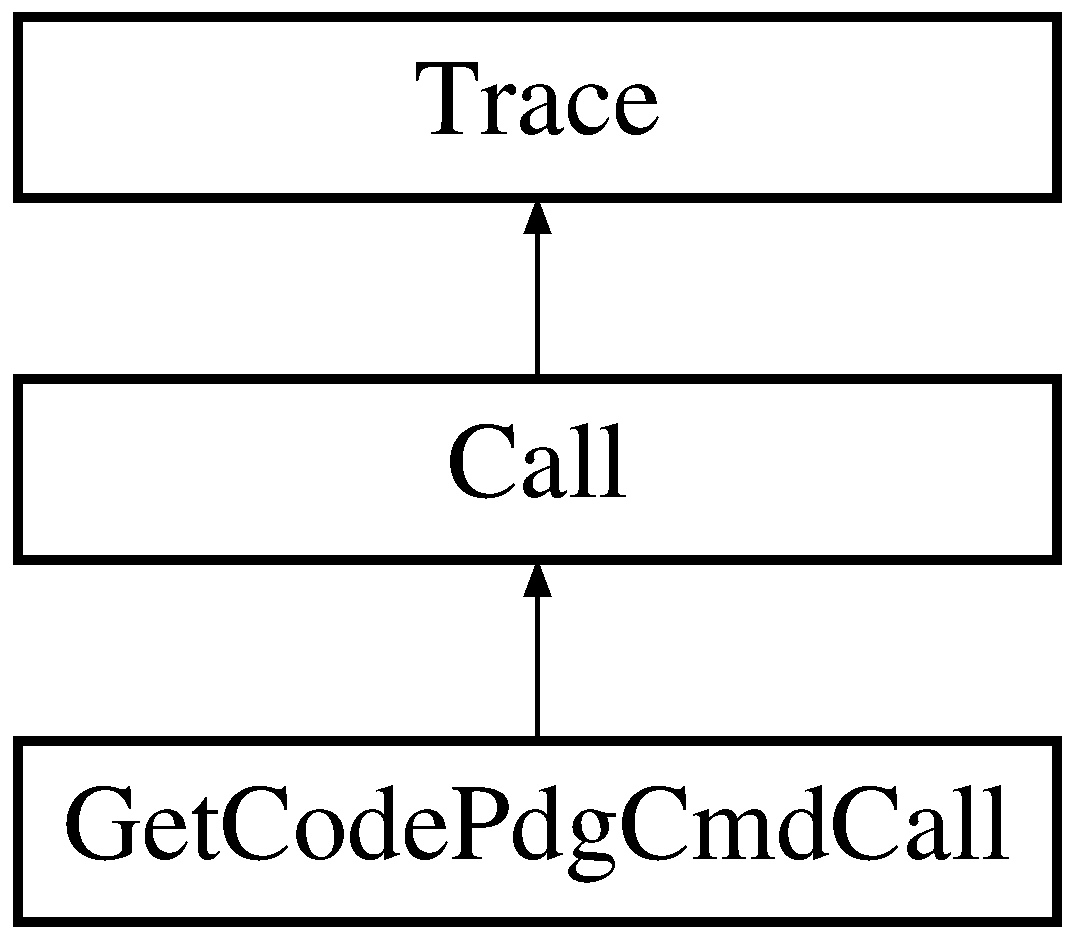
\includegraphics[height=3.000000cm]{class_get_code_pdg_cmd_call}
\end{center}
\end{figure}
\subsection*{Public Member Functions}
\begin{DoxyCompactItemize}
\item 
\hyperlink{class_get_code_pdg_cmd_call_a43634e43855c48ccf4389f5a30634ebc}{Get\+Code\+Pdg\+Cmd\+Call} (\hyperlink{class_call_ade833a08ce215aaa4121102f3448c898}{Error\+Type} \hyperlink{class_call_a206f6150a8038fda48c17c2c7421aed1}{error}, int unit\+Id, int unit\+Type, int id\+Cmd)
\item 
\hyperlink{class_get_code_pdg_cmd_call_adbbbc84d8b72f97363ffdfeb45e6b5ce}{Get\+Code\+Pdg\+Cmd\+Call} (const \hyperlink{class_get_code_pdg_cmd_call}{Get\+Code\+Pdg\+Cmd\+Call} $\ast$c)
\item 
virtual \hyperlink{class_trace_a9c58e523529fc8a03fb6acf3eef86150}{Trace\+::sp\+\_\+trace} \hyperlink{class_get_code_pdg_cmd_call_adad7b71e06c9b81d17b02191401245f5}{clone} () const 
\begin{DoxyCompactList}\small\item\em Clonage d\textquotesingle{}un appel. \end{DoxyCompactList}\end{DoxyCompactItemize}
\subsection*{Additional Inherited Members}


\subsection{Detailed Description}


Definition at line 799 of file Call\+Def.\+h.



\subsection{Constructor \& Destructor Documentation}
\index{Get\+Code\+Pdg\+Cmd\+Call@{Get\+Code\+Pdg\+Cmd\+Call}!Get\+Code\+Pdg\+Cmd\+Call@{Get\+Code\+Pdg\+Cmd\+Call}}
\index{Get\+Code\+Pdg\+Cmd\+Call@{Get\+Code\+Pdg\+Cmd\+Call}!Get\+Code\+Pdg\+Cmd\+Call@{Get\+Code\+Pdg\+Cmd\+Call}}
\subsubsection[{\texorpdfstring{Get\+Code\+Pdg\+Cmd\+Call(\+Error\+Type error, int unit\+Id, int unit\+Type, int id\+Cmd)}{GetCodePdgCmdCall(ErrorType error, int unitId, int unitType, int idCmd)}}]{\setlength{\rightskip}{0pt plus 5cm}Get\+Code\+Pdg\+Cmd\+Call\+::\+Get\+Code\+Pdg\+Cmd\+Call (
\begin{DoxyParamCaption}
\item[{{\bf Error\+Type}}]{error, }
\item[{int}]{unit\+Id, }
\item[{int}]{unit\+Type, }
\item[{int}]{id\+Cmd}
\end{DoxyParamCaption}
)\hspace{0.3cm}{\ttfamily [inline]}}\hypertarget{class_get_code_pdg_cmd_call_a43634e43855c48ccf4389f5a30634ebc}{}\label{class_get_code_pdg_cmd_call_a43634e43855c48ccf4389f5a30634ebc}


Definition at line 803 of file Call\+Def.\+h.

\index{Get\+Code\+Pdg\+Cmd\+Call@{Get\+Code\+Pdg\+Cmd\+Call}!Get\+Code\+Pdg\+Cmd\+Call@{Get\+Code\+Pdg\+Cmd\+Call}}
\index{Get\+Code\+Pdg\+Cmd\+Call@{Get\+Code\+Pdg\+Cmd\+Call}!Get\+Code\+Pdg\+Cmd\+Call@{Get\+Code\+Pdg\+Cmd\+Call}}
\subsubsection[{\texorpdfstring{Get\+Code\+Pdg\+Cmd\+Call(const Get\+Code\+Pdg\+Cmd\+Call $\ast$c)}{GetCodePdgCmdCall(const GetCodePdgCmdCall *c)}}]{\setlength{\rightskip}{0pt plus 5cm}Get\+Code\+Pdg\+Cmd\+Call\+::\+Get\+Code\+Pdg\+Cmd\+Call (
\begin{DoxyParamCaption}
\item[{const {\bf Get\+Code\+Pdg\+Cmd\+Call} $\ast$}]{c}
\end{DoxyParamCaption}
)\hspace{0.3cm}{\ttfamily [inline]}}\hypertarget{class_get_code_pdg_cmd_call_adbbbc84d8b72f97363ffdfeb45e6b5ce}{}\label{class_get_code_pdg_cmd_call_adbbbc84d8b72f97363ffdfeb45e6b5ce}


Definition at line 808 of file Call\+Def.\+h.



\subsection{Member Function Documentation}
\index{Get\+Code\+Pdg\+Cmd\+Call@{Get\+Code\+Pdg\+Cmd\+Call}!clone@{clone}}
\index{clone@{clone}!Get\+Code\+Pdg\+Cmd\+Call@{Get\+Code\+Pdg\+Cmd\+Call}}
\subsubsection[{\texorpdfstring{clone() const }{clone() const }}]{\setlength{\rightskip}{0pt plus 5cm}virtual {\bf Trace\+::sp\+\_\+trace} Get\+Code\+Pdg\+Cmd\+Call\+::clone (
\begin{DoxyParamCaption}
{}
\end{DoxyParamCaption}
) const\hspace{0.3cm}{\ttfamily [inline]}, {\ttfamily [virtual]}}\hypertarget{class_get_code_pdg_cmd_call_adad7b71e06c9b81d17b02191401245f5}{}\label{class_get_code_pdg_cmd_call_adad7b71e06c9b81d17b02191401245f5}


Clonage d\textquotesingle{}un appel. 

\begin{DoxyReturn}{Returns}
une copie de l\textquotesingle{}objet \hyperlink{class_call}{Call}. 
\end{DoxyReturn}


Implements \hyperlink{class_call_ab3bf0965d35eb1e97ecddaf2d3978e9b}{Call}.



Definition at line 814 of file Call\+Def.\+h.



The documentation for this class was generated from the following file\+:\begin{DoxyCompactItemize}
\item 
C\+:/\+Users/\+Stephane/\+Desktop/mocahteam/\+Prog\+And\+Play/pp/traces/src/\hyperlink{_call_def_8h}{Call\+Def.\+h}\end{DoxyCompactItemize}

\hypertarget{class_get_num_params_pdg_cmd_call}{}\section{Get\+Num\+Params\+Pdg\+Cmd\+Call Class Reference}
\label{class_get_num_params_pdg_cmd_call}\index{Get\+Num\+Params\+Pdg\+Cmd\+Call@{Get\+Num\+Params\+Pdg\+Cmd\+Call}}


{\ttfamily \#include $<$Call\+Def.\+h$>$}

Inheritance diagram for Get\+Num\+Params\+Pdg\+Cmd\+Call\+:\begin{figure}[H]
\begin{center}
\leavevmode
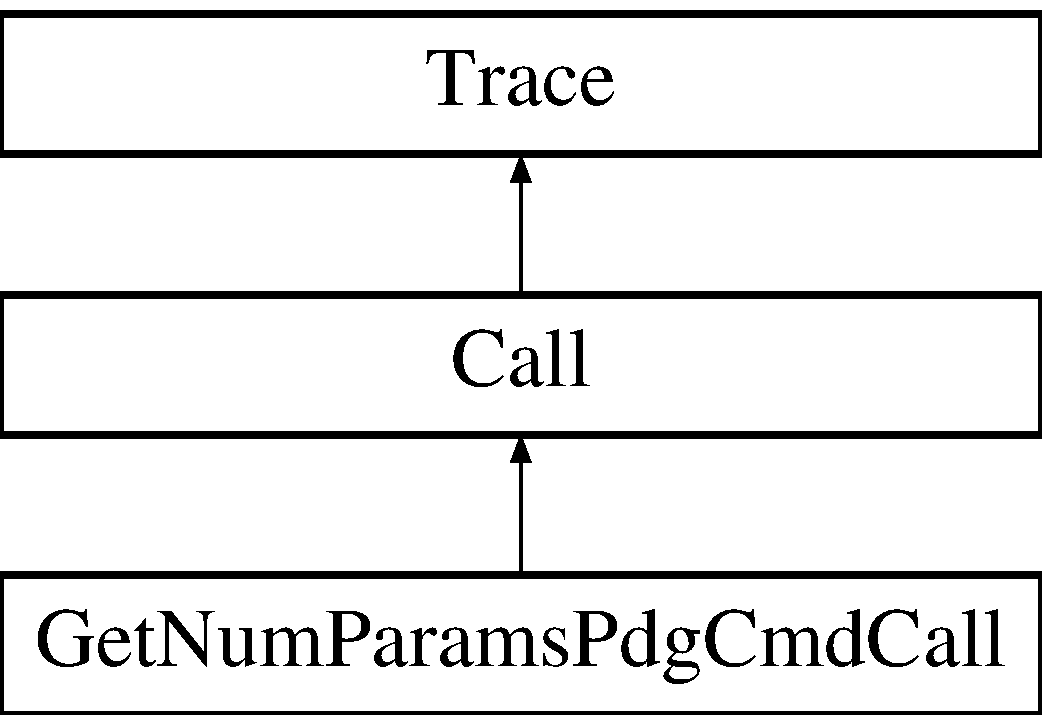
\includegraphics[height=3.000000cm]{class_get_num_params_pdg_cmd_call}
\end{center}
\end{figure}
\subsection*{Public Member Functions}
\begin{DoxyCompactItemize}
\item 
\hyperlink{class_get_num_params_pdg_cmd_call_a4a3f171d64aa75248b1a75a2871bfcb4}{Get\+Num\+Params\+Pdg\+Cmd\+Call} (\hyperlink{class_call_ade833a08ce215aaa4121102f3448c898}{Error\+Type} \hyperlink{class_call_a206f6150a8038fda48c17c2c7421aed1}{error}, int unit\+Id, int unit\+Type, int id\+Cmd)
\item 
\hyperlink{class_get_num_params_pdg_cmd_call_adeba6dd73ce4e1ac191563f545d93ef4}{Get\+Num\+Params\+Pdg\+Cmd\+Call} (const \hyperlink{class_get_num_params_pdg_cmd_call}{Get\+Num\+Params\+Pdg\+Cmd\+Call} $\ast$c)
\item 
virtual \hyperlink{class_trace_a9c58e523529fc8a03fb6acf3eef86150}{Trace\+::sp\+\_\+trace} \hyperlink{class_get_num_params_pdg_cmd_call_ae0633bca77530d2e3ad5bc3a68109c8f}{clone} () const 
\begin{DoxyCompactList}\small\item\em Clonage d\textquotesingle{}un appel. \end{DoxyCompactList}\end{DoxyCompactItemize}
\subsection*{Additional Inherited Members}


\subsection{Detailed Description}


Definition at line 883 of file Call\+Def.\+h.



\subsection{Constructor \& Destructor Documentation}
\index{Get\+Num\+Params\+Pdg\+Cmd\+Call@{Get\+Num\+Params\+Pdg\+Cmd\+Call}!Get\+Num\+Params\+Pdg\+Cmd\+Call@{Get\+Num\+Params\+Pdg\+Cmd\+Call}}
\index{Get\+Num\+Params\+Pdg\+Cmd\+Call@{Get\+Num\+Params\+Pdg\+Cmd\+Call}!Get\+Num\+Params\+Pdg\+Cmd\+Call@{Get\+Num\+Params\+Pdg\+Cmd\+Call}}
\subsubsection[{\texorpdfstring{Get\+Num\+Params\+Pdg\+Cmd\+Call(\+Error\+Type error, int unit\+Id, int unit\+Type, int id\+Cmd)}{GetNumParamsPdgCmdCall(ErrorType error, int unitId, int unitType, int idCmd)}}]{\setlength{\rightskip}{0pt plus 5cm}Get\+Num\+Params\+Pdg\+Cmd\+Call\+::\+Get\+Num\+Params\+Pdg\+Cmd\+Call (
\begin{DoxyParamCaption}
\item[{{\bf Error\+Type}}]{error, }
\item[{int}]{unit\+Id, }
\item[{int}]{unit\+Type, }
\item[{int}]{id\+Cmd}
\end{DoxyParamCaption}
)\hspace{0.3cm}{\ttfamily [inline]}}\hypertarget{class_get_num_params_pdg_cmd_call_a4a3f171d64aa75248b1a75a2871bfcb4}{}\label{class_get_num_params_pdg_cmd_call_a4a3f171d64aa75248b1a75a2871bfcb4}


Definition at line 887 of file Call\+Def.\+h.

\index{Get\+Num\+Params\+Pdg\+Cmd\+Call@{Get\+Num\+Params\+Pdg\+Cmd\+Call}!Get\+Num\+Params\+Pdg\+Cmd\+Call@{Get\+Num\+Params\+Pdg\+Cmd\+Call}}
\index{Get\+Num\+Params\+Pdg\+Cmd\+Call@{Get\+Num\+Params\+Pdg\+Cmd\+Call}!Get\+Num\+Params\+Pdg\+Cmd\+Call@{Get\+Num\+Params\+Pdg\+Cmd\+Call}}
\subsubsection[{\texorpdfstring{Get\+Num\+Params\+Pdg\+Cmd\+Call(const Get\+Num\+Params\+Pdg\+Cmd\+Call $\ast$c)}{GetNumParamsPdgCmdCall(const GetNumParamsPdgCmdCall *c)}}]{\setlength{\rightskip}{0pt plus 5cm}Get\+Num\+Params\+Pdg\+Cmd\+Call\+::\+Get\+Num\+Params\+Pdg\+Cmd\+Call (
\begin{DoxyParamCaption}
\item[{const {\bf Get\+Num\+Params\+Pdg\+Cmd\+Call} $\ast$}]{c}
\end{DoxyParamCaption}
)\hspace{0.3cm}{\ttfamily [inline]}}\hypertarget{class_get_num_params_pdg_cmd_call_adeba6dd73ce4e1ac191563f545d93ef4}{}\label{class_get_num_params_pdg_cmd_call_adeba6dd73ce4e1ac191563f545d93ef4}


Definition at line 892 of file Call\+Def.\+h.



\subsection{Member Function Documentation}
\index{Get\+Num\+Params\+Pdg\+Cmd\+Call@{Get\+Num\+Params\+Pdg\+Cmd\+Call}!clone@{clone}}
\index{clone@{clone}!Get\+Num\+Params\+Pdg\+Cmd\+Call@{Get\+Num\+Params\+Pdg\+Cmd\+Call}}
\subsubsection[{\texorpdfstring{clone() const }{clone() const }}]{\setlength{\rightskip}{0pt plus 5cm}virtual {\bf Trace\+::sp\+\_\+trace} Get\+Num\+Params\+Pdg\+Cmd\+Call\+::clone (
\begin{DoxyParamCaption}
{}
\end{DoxyParamCaption}
) const\hspace{0.3cm}{\ttfamily [inline]}, {\ttfamily [virtual]}}\hypertarget{class_get_num_params_pdg_cmd_call_ae0633bca77530d2e3ad5bc3a68109c8f}{}\label{class_get_num_params_pdg_cmd_call_ae0633bca77530d2e3ad5bc3a68109c8f}


Clonage d\textquotesingle{}un appel. 

\begin{DoxyReturn}{Returns}
une copie de l\textquotesingle{}objet \hyperlink{class_call}{Call}. 
\end{DoxyReturn}


Implements \hyperlink{class_call_ab3bf0965d35eb1e97ecddaf2d3978e9b}{Call}.



Definition at line 898 of file Call\+Def.\+h.



The documentation for this class was generated from the following file\+:\begin{DoxyCompactItemize}
\item 
C\+:/\+Users/\+Stephane/\+Desktop/mocahteam/\+Prog\+And\+Play/pp/traces/src/\hyperlink{_call_def_8h}{Call\+Def.\+h}\end{DoxyCompactItemize}

\hypertarget{class_get_num_units_call}{}\section{Get\+Num\+Units\+Call Class Reference}
\label{class_get_num_units_call}\index{Get\+Num\+Units\+Call@{Get\+Num\+Units\+Call}}


{\ttfamily \#include $<$Call\+Def.\+h$>$}

Inheritance diagram for Get\+Num\+Units\+Call\+:\begin{figure}[H]
\begin{center}
\leavevmode
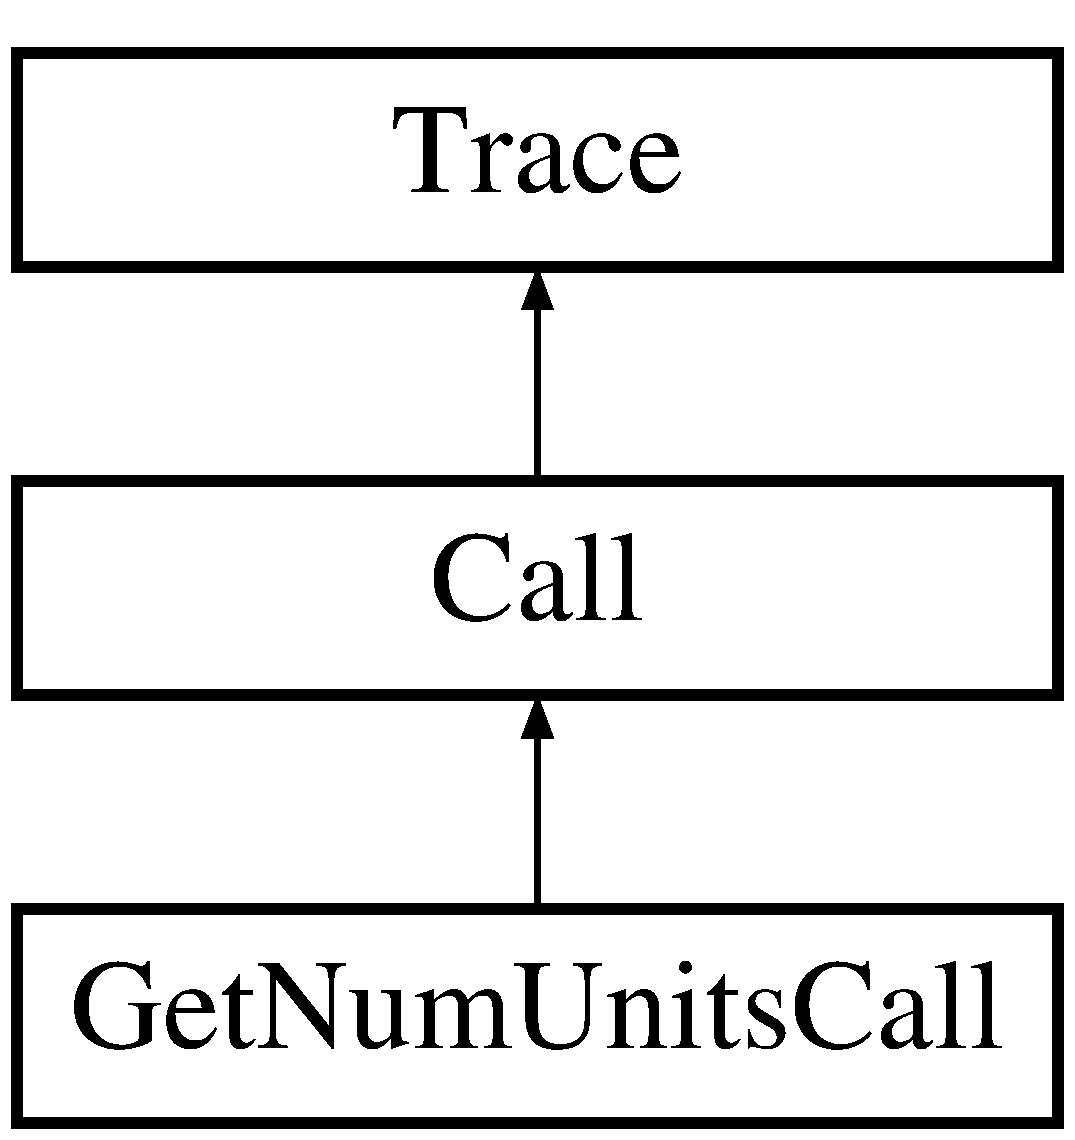
\includegraphics[height=3.000000cm]{class_get_num_units_call}
\end{center}
\end{figure}
\subsection*{Public Member Functions}
\begin{DoxyCompactItemize}
\item 
\hyperlink{class_get_num_units_call_a093f1ca9dcd35921b62fc1e23fb315e7}{Get\+Num\+Units\+Call} (\hyperlink{class_call_ade833a08ce215aaa4121102f3448c898}{Error\+Type} \hyperlink{class_call_a206f6150a8038fda48c17c2c7421aed1}{error}, \hyperlink{namespace_call_misc_a490b3c2ef1a821675848ebcab0b677d8}{Call\+Misc\+::\+Coalition} coalition)
\item 
\hyperlink{class_get_num_units_call_ae85cafa25d8c81e510df0694f770e37a}{Get\+Num\+Units\+Call} (const \hyperlink{class_get_num_units_call}{Get\+Num\+Units\+Call} $\ast$c)
\item 
virtual \hyperlink{class_trace_a9c58e523529fc8a03fb6acf3eef86150}{Trace\+::sp\+\_\+trace} \hyperlink{class_get_num_units_call_a279250063949139d58842ae5a6b39b03}{clone} () const 
\begin{DoxyCompactList}\small\item\em Clonage d\textquotesingle{}un appel. \end{DoxyCompactList}\end{DoxyCompactItemize}
\subsection*{Additional Inherited Members}


\subsection{Detailed Description}


Definition at line 205 of file Call\+Def.\+h.



\subsection{Constructor \& Destructor Documentation}
\index{Get\+Num\+Units\+Call@{Get\+Num\+Units\+Call}!Get\+Num\+Units\+Call@{Get\+Num\+Units\+Call}}
\index{Get\+Num\+Units\+Call@{Get\+Num\+Units\+Call}!Get\+Num\+Units\+Call@{Get\+Num\+Units\+Call}}
\subsubsection[{\texorpdfstring{Get\+Num\+Units\+Call(\+Error\+Type error, Call\+Misc\+::\+Coalition coalition)}{GetNumUnitsCall(ErrorType error, CallMisc::Coalition coalition)}}]{\setlength{\rightskip}{0pt plus 5cm}Get\+Num\+Units\+Call\+::\+Get\+Num\+Units\+Call (
\begin{DoxyParamCaption}
\item[{{\bf Error\+Type}}]{error, }
\item[{{\bf Call\+Misc\+::\+Coalition}}]{coalition}
\end{DoxyParamCaption}
)\hspace{0.3cm}{\ttfamily [inline]}}\hypertarget{class_get_num_units_call_a093f1ca9dcd35921b62fc1e23fb315e7}{}\label{class_get_num_units_call_a093f1ca9dcd35921b62fc1e23fb315e7}


Definition at line 209 of file Call\+Def.\+h.

\index{Get\+Num\+Units\+Call@{Get\+Num\+Units\+Call}!Get\+Num\+Units\+Call@{Get\+Num\+Units\+Call}}
\index{Get\+Num\+Units\+Call@{Get\+Num\+Units\+Call}!Get\+Num\+Units\+Call@{Get\+Num\+Units\+Call}}
\subsubsection[{\texorpdfstring{Get\+Num\+Units\+Call(const Get\+Num\+Units\+Call $\ast$c)}{GetNumUnitsCall(const GetNumUnitsCall *c)}}]{\setlength{\rightskip}{0pt plus 5cm}Get\+Num\+Units\+Call\+::\+Get\+Num\+Units\+Call (
\begin{DoxyParamCaption}
\item[{const {\bf Get\+Num\+Units\+Call} $\ast$}]{c}
\end{DoxyParamCaption}
)\hspace{0.3cm}{\ttfamily [inline]}}\hypertarget{class_get_num_units_call_ae85cafa25d8c81e510df0694f770e37a}{}\label{class_get_num_units_call_ae85cafa25d8c81e510df0694f770e37a}


Definition at line 211 of file Call\+Def.\+h.



\subsection{Member Function Documentation}
\index{Get\+Num\+Units\+Call@{Get\+Num\+Units\+Call}!clone@{clone}}
\index{clone@{clone}!Get\+Num\+Units\+Call@{Get\+Num\+Units\+Call}}
\subsubsection[{\texorpdfstring{clone() const }{clone() const }}]{\setlength{\rightskip}{0pt plus 5cm}virtual {\bf Trace\+::sp\+\_\+trace} Get\+Num\+Units\+Call\+::clone (
\begin{DoxyParamCaption}
{}
\end{DoxyParamCaption}
) const\hspace{0.3cm}{\ttfamily [inline]}, {\ttfamily [virtual]}}\hypertarget{class_get_num_units_call_a279250063949139d58842ae5a6b39b03}{}\label{class_get_num_units_call_a279250063949139d58842ae5a6b39b03}


Clonage d\textquotesingle{}un appel. 

\begin{DoxyReturn}{Returns}
une copie de l\textquotesingle{}objet \hyperlink{class_call}{Call}. 
\end{DoxyReturn}


Implements \hyperlink{class_call_ab3bf0965d35eb1e97ecddaf2d3978e9b}{Call}.



Definition at line 215 of file Call\+Def.\+h.



The documentation for this class was generated from the following file\+:\begin{DoxyCompactItemize}
\item 
C\+:/\+Users/\+Stephane/\+Desktop/mocahteam/\+Prog\+And\+Play/pp/traces/src/\hyperlink{_call_def_8h}{Call\+Def.\+h}\end{DoxyCompactItemize}

\hypertarget{class_get_param_pdg_cmd_call}{}\section{Get\+Param\+Pdg\+Cmd\+Call Class Reference}
\label{class_get_param_pdg_cmd_call}\index{Get\+Param\+Pdg\+Cmd\+Call@{Get\+Param\+Pdg\+Cmd\+Call}}


{\ttfamily \#include $<$Call\+Def.\+h$>$}

Inheritance diagram for Get\+Param\+Pdg\+Cmd\+Call\+:\begin{figure}[H]
\begin{center}
\leavevmode
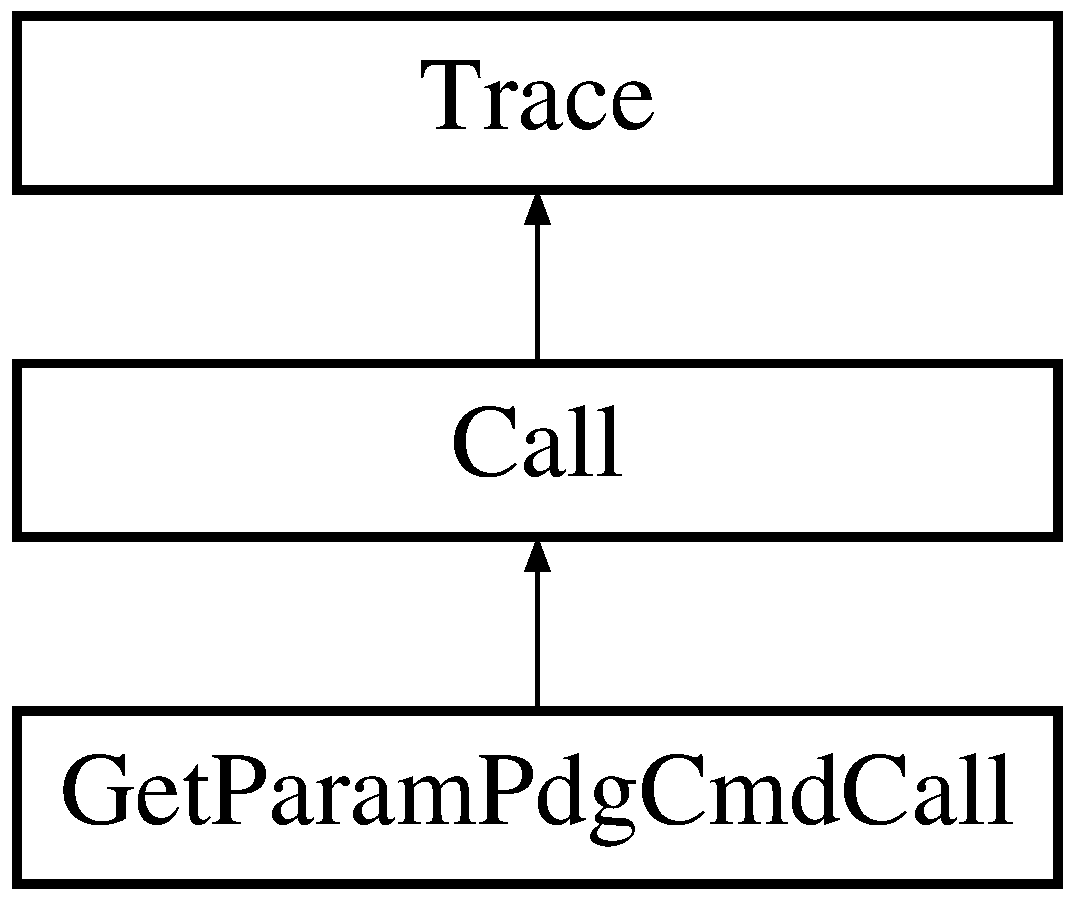
\includegraphics[height=3.000000cm]{class_get_param_pdg_cmd_call}
\end{center}
\end{figure}
\subsection*{Public Member Functions}
\begin{DoxyCompactItemize}
\item 
\hyperlink{class_get_param_pdg_cmd_call_a26b970d28a2942b08bc9605ddc0b21ce}{Get\+Param\+Pdg\+Cmd\+Call} (\hyperlink{class_call_ade833a08ce215aaa4121102f3448c898}{Error\+Type} \hyperlink{class_call_a206f6150a8038fda48c17c2c7421aed1}{error}, int unit\+Id, int unit\+Type, int id\+Cmd, int id\+Param)
\item 
\hyperlink{class_get_param_pdg_cmd_call_aff03cad7f19271a5f07602f6a3b08201}{Get\+Param\+Pdg\+Cmd\+Call} (const \hyperlink{class_get_param_pdg_cmd_call}{Get\+Param\+Pdg\+Cmd\+Call} $\ast$c)
\item 
virtual \hyperlink{class_trace_a9c58e523529fc8a03fb6acf3eef86150}{Trace\+::sp\+\_\+trace} \hyperlink{class_get_param_pdg_cmd_call_a07b0bec23a831830746b25ca5d44b317}{clone} () const 
\begin{DoxyCompactList}\small\item\em Clonage d\textquotesingle{}un appel. \end{DoxyCompactList}\end{DoxyCompactItemize}
\subsection*{Additional Inherited Members}


\subsection{Detailed Description}


Definition at line 967 of file Call\+Def.\+h.



\subsection{Constructor \& Destructor Documentation}
\index{Get\+Param\+Pdg\+Cmd\+Call@{Get\+Param\+Pdg\+Cmd\+Call}!Get\+Param\+Pdg\+Cmd\+Call@{Get\+Param\+Pdg\+Cmd\+Call}}
\index{Get\+Param\+Pdg\+Cmd\+Call@{Get\+Param\+Pdg\+Cmd\+Call}!Get\+Param\+Pdg\+Cmd\+Call@{Get\+Param\+Pdg\+Cmd\+Call}}
\subsubsection[{\texorpdfstring{Get\+Param\+Pdg\+Cmd\+Call(\+Error\+Type error, int unit\+Id, int unit\+Type, int id\+Cmd, int id\+Param)}{GetParamPdgCmdCall(ErrorType error, int unitId, int unitType, int idCmd, int idParam)}}]{\setlength{\rightskip}{0pt plus 5cm}Get\+Param\+Pdg\+Cmd\+Call\+::\+Get\+Param\+Pdg\+Cmd\+Call (
\begin{DoxyParamCaption}
\item[{{\bf Error\+Type}}]{error, }
\item[{int}]{unit\+Id, }
\item[{int}]{unit\+Type, }
\item[{int}]{id\+Cmd, }
\item[{int}]{id\+Param}
\end{DoxyParamCaption}
)\hspace{0.3cm}{\ttfamily [inline]}}\hypertarget{class_get_param_pdg_cmd_call_a26b970d28a2942b08bc9605ddc0b21ce}{}\label{class_get_param_pdg_cmd_call_a26b970d28a2942b08bc9605ddc0b21ce}


Definition at line 971 of file Call\+Def.\+h.

\index{Get\+Param\+Pdg\+Cmd\+Call@{Get\+Param\+Pdg\+Cmd\+Call}!Get\+Param\+Pdg\+Cmd\+Call@{Get\+Param\+Pdg\+Cmd\+Call}}
\index{Get\+Param\+Pdg\+Cmd\+Call@{Get\+Param\+Pdg\+Cmd\+Call}!Get\+Param\+Pdg\+Cmd\+Call@{Get\+Param\+Pdg\+Cmd\+Call}}
\subsubsection[{\texorpdfstring{Get\+Param\+Pdg\+Cmd\+Call(const Get\+Param\+Pdg\+Cmd\+Call $\ast$c)}{GetParamPdgCmdCall(const GetParamPdgCmdCall *c)}}]{\setlength{\rightskip}{0pt plus 5cm}Get\+Param\+Pdg\+Cmd\+Call\+::\+Get\+Param\+Pdg\+Cmd\+Call (
\begin{DoxyParamCaption}
\item[{const {\bf Get\+Param\+Pdg\+Cmd\+Call} $\ast$}]{c}
\end{DoxyParamCaption}
)\hspace{0.3cm}{\ttfamily [inline]}}\hypertarget{class_get_param_pdg_cmd_call_aff03cad7f19271a5f07602f6a3b08201}{}\label{class_get_param_pdg_cmd_call_aff03cad7f19271a5f07602f6a3b08201}


Definition at line 976 of file Call\+Def.\+h.



\subsection{Member Function Documentation}
\index{Get\+Param\+Pdg\+Cmd\+Call@{Get\+Param\+Pdg\+Cmd\+Call}!clone@{clone}}
\index{clone@{clone}!Get\+Param\+Pdg\+Cmd\+Call@{Get\+Param\+Pdg\+Cmd\+Call}}
\subsubsection[{\texorpdfstring{clone() const }{clone() const }}]{\setlength{\rightskip}{0pt plus 5cm}virtual {\bf Trace\+::sp\+\_\+trace} Get\+Param\+Pdg\+Cmd\+Call\+::clone (
\begin{DoxyParamCaption}
{}
\end{DoxyParamCaption}
) const\hspace{0.3cm}{\ttfamily [inline]}, {\ttfamily [virtual]}}\hypertarget{class_get_param_pdg_cmd_call_a07b0bec23a831830746b25ca5d44b317}{}\label{class_get_param_pdg_cmd_call_a07b0bec23a831830746b25ca5d44b317}


Clonage d\textquotesingle{}un appel. 

\begin{DoxyReturn}{Returns}
une copie de l\textquotesingle{}objet \hyperlink{class_call}{Call}. 
\end{DoxyReturn}


Implements \hyperlink{class_call_ab3bf0965d35eb1e97ecddaf2d3978e9b}{Call}.



Definition at line 983 of file Call\+Def.\+h.



The documentation for this class was generated from the following file\+:\begin{DoxyCompactItemize}
\item 
C\+:/\+Users/\+Stephane/\+Desktop/mocahteam/\+Prog\+And\+Play/pp/traces/src/\hyperlink{_call_def_8h}{Call\+Def.\+h}\end{DoxyCompactItemize}

\hypertarget{class_get_resource_call}{}\section{Get\+Resource\+Call Class Reference}
\label{class_get_resource_call}\index{Get\+Resource\+Call@{Get\+Resource\+Call}}


{\ttfamily \#include $<$Call\+Def.\+h$>$}

Inheritance diagram for Get\+Resource\+Call\+:\begin{figure}[H]
\begin{center}
\leavevmode
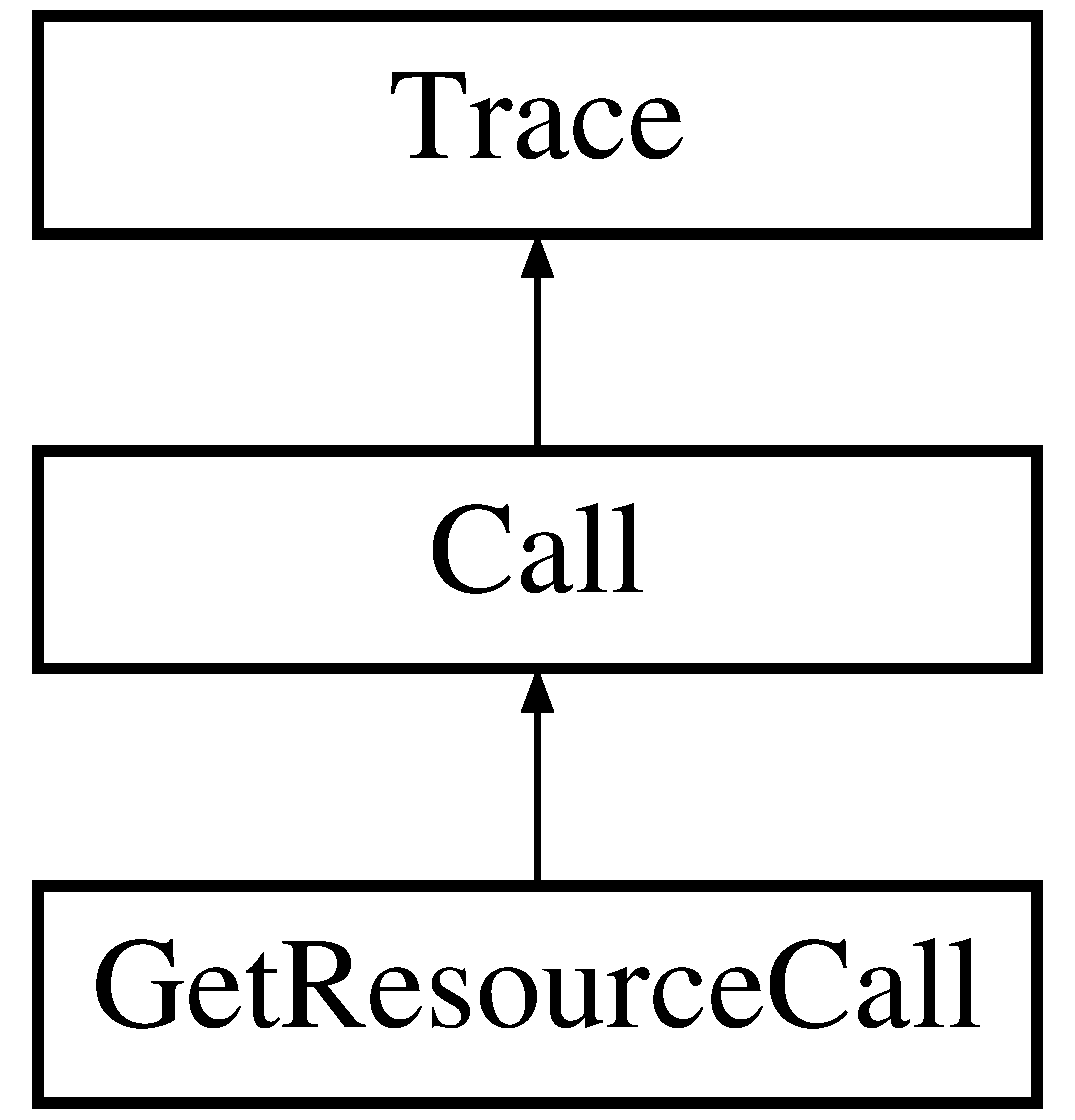
\includegraphics[height=3.000000cm]{class_get_resource_call}
\end{center}
\end{figure}
\subsection*{Public Member Functions}
\begin{DoxyCompactItemize}
\item 
\hyperlink{class_get_resource_call_aad3bb58fedeed2204ed45537021bb696}{Get\+Resource\+Call} (\hyperlink{class_call_ade833a08ce215aaa4121102f3448c898}{Error\+Type} \hyperlink{class_call_a206f6150a8038fda48c17c2c7421aed1}{error}, int resource\+Id)
\item 
\hyperlink{class_get_resource_call_a1ee622f0e449e11767b9054a46d50f87}{Get\+Resource\+Call} (const \hyperlink{class_get_resource_call}{Get\+Resource\+Call} $\ast$c)
\item 
virtual \hyperlink{class_trace_a9c58e523529fc8a03fb6acf3eef86150}{Trace\+::sp\+\_\+trace} \hyperlink{class_get_resource_call_adeda1479826fb33c27c76bd8fe711776}{clone} () const 
\begin{DoxyCompactList}\small\item\em Clonage d\textquotesingle{}un appel. \end{DoxyCompactList}\end{DoxyCompactItemize}
\subsection*{Additional Inherited Members}


\subsection{Detailed Description}


Definition at line 145 of file Call\+Def.\+h.



\subsection{Constructor \& Destructor Documentation}
\index{Get\+Resource\+Call@{Get\+Resource\+Call}!Get\+Resource\+Call@{Get\+Resource\+Call}}
\index{Get\+Resource\+Call@{Get\+Resource\+Call}!Get\+Resource\+Call@{Get\+Resource\+Call}}
\subsubsection[{\texorpdfstring{Get\+Resource\+Call(\+Error\+Type error, int resource\+Id)}{GetResourceCall(ErrorType error, int resourceId)}}]{\setlength{\rightskip}{0pt plus 5cm}Get\+Resource\+Call\+::\+Get\+Resource\+Call (
\begin{DoxyParamCaption}
\item[{{\bf Error\+Type}}]{error, }
\item[{int}]{resource\+Id}
\end{DoxyParamCaption}
)\hspace{0.3cm}{\ttfamily [inline]}}\hypertarget{class_get_resource_call_aad3bb58fedeed2204ed45537021bb696}{}\label{class_get_resource_call_aad3bb58fedeed2204ed45537021bb696}


Definition at line 149 of file Call\+Def.\+h.

\index{Get\+Resource\+Call@{Get\+Resource\+Call}!Get\+Resource\+Call@{Get\+Resource\+Call}}
\index{Get\+Resource\+Call@{Get\+Resource\+Call}!Get\+Resource\+Call@{Get\+Resource\+Call}}
\subsubsection[{\texorpdfstring{Get\+Resource\+Call(const Get\+Resource\+Call $\ast$c)}{GetResourceCall(const GetResourceCall *c)}}]{\setlength{\rightskip}{0pt plus 5cm}Get\+Resource\+Call\+::\+Get\+Resource\+Call (
\begin{DoxyParamCaption}
\item[{const {\bf Get\+Resource\+Call} $\ast$}]{c}
\end{DoxyParamCaption}
)\hspace{0.3cm}{\ttfamily [inline]}}\hypertarget{class_get_resource_call_a1ee622f0e449e11767b9054a46d50f87}{}\label{class_get_resource_call_a1ee622f0e449e11767b9054a46d50f87}


Definition at line 151 of file Call\+Def.\+h.



\subsection{Member Function Documentation}
\index{Get\+Resource\+Call@{Get\+Resource\+Call}!clone@{clone}}
\index{clone@{clone}!Get\+Resource\+Call@{Get\+Resource\+Call}}
\subsubsection[{\texorpdfstring{clone() const }{clone() const }}]{\setlength{\rightskip}{0pt plus 5cm}virtual {\bf Trace\+::sp\+\_\+trace} Get\+Resource\+Call\+::clone (
\begin{DoxyParamCaption}
{}
\end{DoxyParamCaption}
) const\hspace{0.3cm}{\ttfamily [inline]}, {\ttfamily [virtual]}}\hypertarget{class_get_resource_call_adeda1479826fb33c27c76bd8fe711776}{}\label{class_get_resource_call_adeda1479826fb33c27c76bd8fe711776}


Clonage d\textquotesingle{}un appel. 

\begin{DoxyReturn}{Returns}
une copie de l\textquotesingle{}objet \hyperlink{class_call}{Call}. 
\end{DoxyReturn}


Implements \hyperlink{class_call_ab3bf0965d35eb1e97ecddaf2d3978e9b}{Call}.



Definition at line 155 of file Call\+Def.\+h.



The documentation for this class was generated from the following file\+:\begin{DoxyCompactItemize}
\item 
C\+:/\+Users/\+Stephane/\+Desktop/mocahteam/\+Prog\+And\+Play/pp/traces/src/\hyperlink{_call_def_8h}{Call\+Def.\+h}\end{DoxyCompactItemize}

\hypertarget{class_get_special_area_position_call}{}\section{Get\+Special\+Area\+Position\+Call Class Reference}
\label{class_get_special_area_position_call}\index{Get\+Special\+Area\+Position\+Call@{Get\+Special\+Area\+Position\+Call}}


{\ttfamily \#include $<$Call\+Def.\+h$>$}

Inheritance diagram for Get\+Special\+Area\+Position\+Call\+:\begin{figure}[H]
\begin{center}
\leavevmode
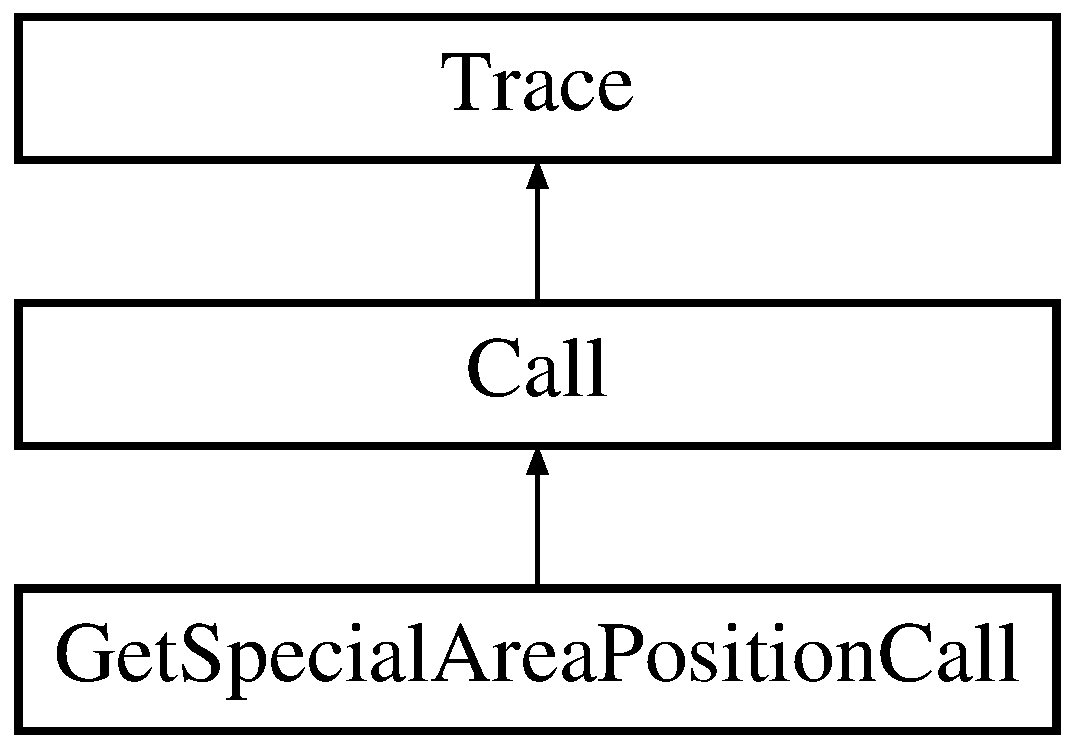
\includegraphics[height=3.000000cm]{class_get_special_area_position_call}
\end{center}
\end{figure}
\subsection*{Public Member Functions}
\begin{DoxyCompactItemize}
\item 
\hyperlink{class_get_special_area_position_call_a518d1a74534bb215e79efb6b946deb6e}{Get\+Special\+Area\+Position\+Call} (\hyperlink{class_call_ade833a08ce215aaa4121102f3448c898}{Error\+Type} \hyperlink{class_call_a206f6150a8038fda48c17c2c7421aed1}{error}, int special\+Area\+Id)
\item 
\hyperlink{class_get_special_area_position_call_a8ee59a88084c9bd9d3db3481d61cd307}{Get\+Special\+Area\+Position\+Call} (const \hyperlink{class_get_special_area_position_call}{Get\+Special\+Area\+Position\+Call} $\ast$c)
\item 
virtual \hyperlink{class_trace_a9c58e523529fc8a03fb6acf3eef86150}{Trace\+::sp\+\_\+trace} \hyperlink{class_get_special_area_position_call_ad522313dad00572f50f2a4a84e12dafd}{clone} () const 
\begin{DoxyCompactList}\small\item\em Clonage d\textquotesingle{}un appel. \end{DoxyCompactList}\end{DoxyCompactItemize}
\subsection*{Additional Inherited Members}


\subsection{Detailed Description}


Definition at line 85 of file Call\+Def.\+h.



\subsection{Constructor \& Destructor Documentation}
\index{Get\+Special\+Area\+Position\+Call@{Get\+Special\+Area\+Position\+Call}!Get\+Special\+Area\+Position\+Call@{Get\+Special\+Area\+Position\+Call}}
\index{Get\+Special\+Area\+Position\+Call@{Get\+Special\+Area\+Position\+Call}!Get\+Special\+Area\+Position\+Call@{Get\+Special\+Area\+Position\+Call}}
\subsubsection[{\texorpdfstring{Get\+Special\+Area\+Position\+Call(\+Error\+Type error, int special\+Area\+Id)}{GetSpecialAreaPositionCall(ErrorType error, int specialAreaId)}}]{\setlength{\rightskip}{0pt plus 5cm}Get\+Special\+Area\+Position\+Call\+::\+Get\+Special\+Area\+Position\+Call (
\begin{DoxyParamCaption}
\item[{{\bf Error\+Type}}]{error, }
\item[{int}]{special\+Area\+Id}
\end{DoxyParamCaption}
)\hspace{0.3cm}{\ttfamily [inline]}}\hypertarget{class_get_special_area_position_call_a518d1a74534bb215e79efb6b946deb6e}{}\label{class_get_special_area_position_call_a518d1a74534bb215e79efb6b946deb6e}


Definition at line 89 of file Call\+Def.\+h.

\index{Get\+Special\+Area\+Position\+Call@{Get\+Special\+Area\+Position\+Call}!Get\+Special\+Area\+Position\+Call@{Get\+Special\+Area\+Position\+Call}}
\index{Get\+Special\+Area\+Position\+Call@{Get\+Special\+Area\+Position\+Call}!Get\+Special\+Area\+Position\+Call@{Get\+Special\+Area\+Position\+Call}}
\subsubsection[{\texorpdfstring{Get\+Special\+Area\+Position\+Call(const Get\+Special\+Area\+Position\+Call $\ast$c)}{GetSpecialAreaPositionCall(const GetSpecialAreaPositionCall *c)}}]{\setlength{\rightskip}{0pt plus 5cm}Get\+Special\+Area\+Position\+Call\+::\+Get\+Special\+Area\+Position\+Call (
\begin{DoxyParamCaption}
\item[{const {\bf Get\+Special\+Area\+Position\+Call} $\ast$}]{c}
\end{DoxyParamCaption}
)\hspace{0.3cm}{\ttfamily [inline]}}\hypertarget{class_get_special_area_position_call_a8ee59a88084c9bd9d3db3481d61cd307}{}\label{class_get_special_area_position_call_a8ee59a88084c9bd9d3db3481d61cd307}


Definition at line 91 of file Call\+Def.\+h.



\subsection{Member Function Documentation}
\index{Get\+Special\+Area\+Position\+Call@{Get\+Special\+Area\+Position\+Call}!clone@{clone}}
\index{clone@{clone}!Get\+Special\+Area\+Position\+Call@{Get\+Special\+Area\+Position\+Call}}
\subsubsection[{\texorpdfstring{clone() const }{clone() const }}]{\setlength{\rightskip}{0pt plus 5cm}virtual {\bf Trace\+::sp\+\_\+trace} Get\+Special\+Area\+Position\+Call\+::clone (
\begin{DoxyParamCaption}
{}
\end{DoxyParamCaption}
) const\hspace{0.3cm}{\ttfamily [inline]}, {\ttfamily [virtual]}}\hypertarget{class_get_special_area_position_call_ad522313dad00572f50f2a4a84e12dafd}{}\label{class_get_special_area_position_call_ad522313dad00572f50f2a4a84e12dafd}


Clonage d\textquotesingle{}un appel. 

\begin{DoxyReturn}{Returns}
une copie de l\textquotesingle{}objet \hyperlink{class_call}{Call}. 
\end{DoxyReturn}


Implements \hyperlink{class_call_ab3bf0965d35eb1e97ecddaf2d3978e9b}{Call}.



Definition at line 95 of file Call\+Def.\+h.



The documentation for this class was generated from the following file\+:\begin{DoxyCompactItemize}
\item 
C\+:/\+Users/\+Stephane/\+Desktop/mocahteam/\+Prog\+And\+Play/pp/traces/src/\hyperlink{_call_def_8h}{Call\+Def.\+h}\end{DoxyCompactItemize}

\hypertarget{class_get_unit_at_call}{}\section{Get\+Unit\+At\+Call Class Reference}
\label{class_get_unit_at_call}\index{Get\+Unit\+At\+Call@{Get\+Unit\+At\+Call}}


{\ttfamily \#include $<$Call\+Def.\+h$>$}

Inheritance diagram for Get\+Unit\+At\+Call\+:\begin{figure}[H]
\begin{center}
\leavevmode
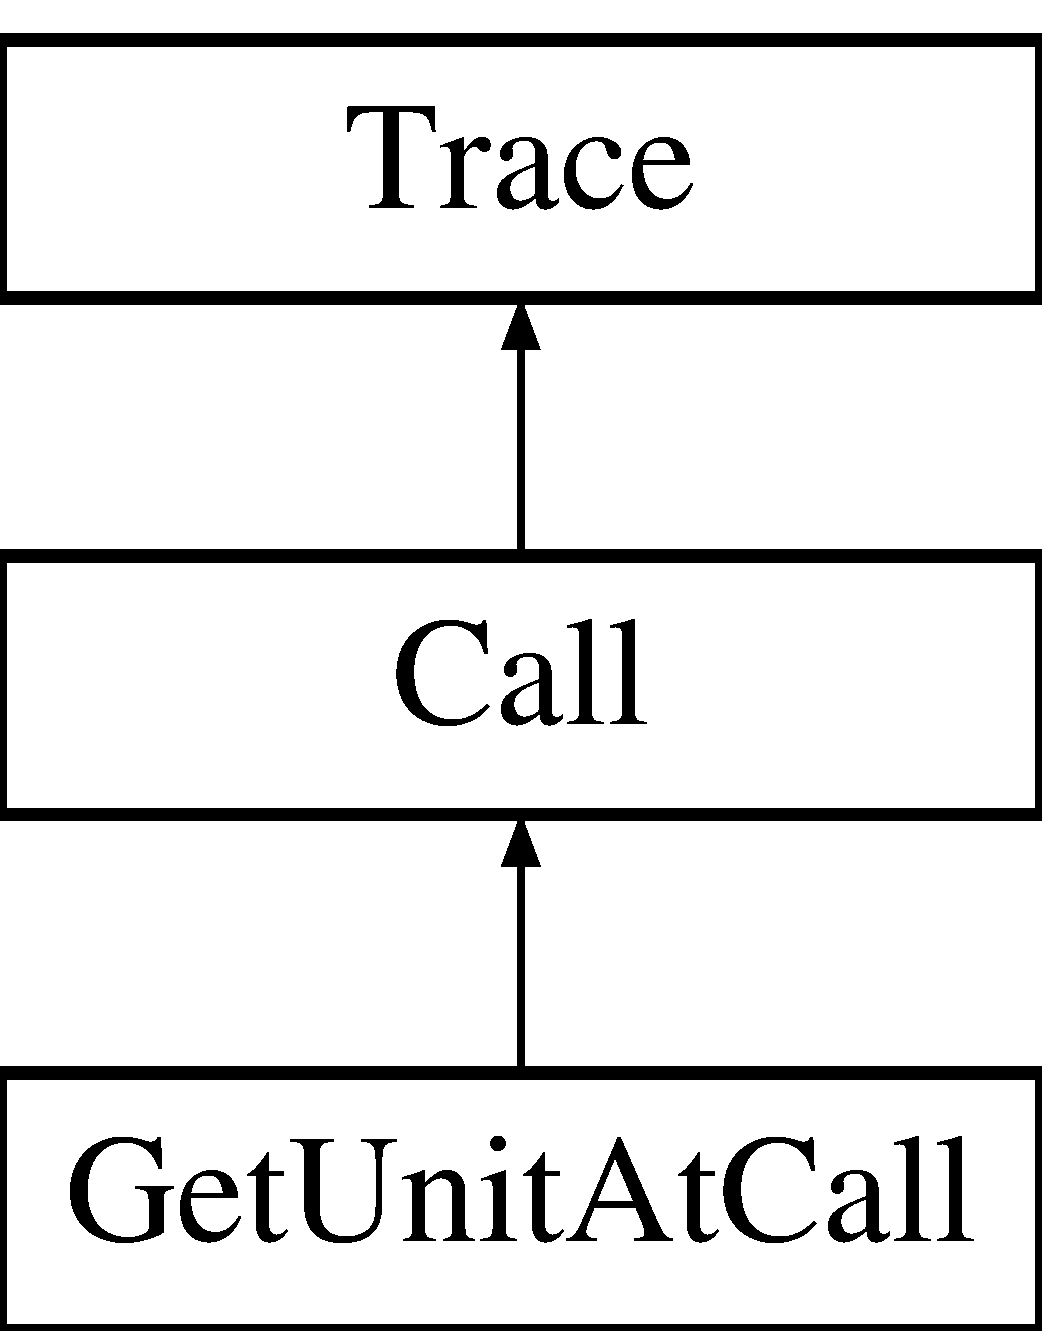
\includegraphics[height=3.000000cm]{class_get_unit_at_call}
\end{center}
\end{figure}
\subsection*{Public Member Functions}
\begin{DoxyCompactItemize}
\item 
\hyperlink{class_get_unit_at_call_a79690d8748e9c015991143cdef23bcfb}{Get\+Unit\+At\+Call} (\hyperlink{class_call_ade833a08ce215aaa4121102f3448c898}{Error\+Type} \hyperlink{class_call_a206f6150a8038fda48c17c2c7421aed1}{error}, \hyperlink{namespace_call_misc_a490b3c2ef1a821675848ebcab0b677d8}{Call\+Misc\+::\+Coalition} coalition, int index)
\item 
\hyperlink{class_get_unit_at_call_a7b3aebc0b99a514aac2b265e8130f8ab}{Get\+Unit\+At\+Call} (const \hyperlink{class_get_unit_at_call}{Get\+Unit\+At\+Call} $\ast$c)
\item 
virtual \hyperlink{class_trace_a9c58e523529fc8a03fb6acf3eef86150}{Trace\+::sp\+\_\+trace} \hyperlink{class_get_unit_at_call_a228108026f5f8522a6724e1183e1b6bb}{clone} () const 
\begin{DoxyCompactList}\small\item\em Clonage d\textquotesingle{}un appel. \end{DoxyCompactList}\end{DoxyCompactItemize}
\subsection*{Additional Inherited Members}


\subsection{Detailed Description}


Definition at line 265 of file Call\+Def.\+h.



\subsection{Constructor \& Destructor Documentation}
\index{Get\+Unit\+At\+Call@{Get\+Unit\+At\+Call}!Get\+Unit\+At\+Call@{Get\+Unit\+At\+Call}}
\index{Get\+Unit\+At\+Call@{Get\+Unit\+At\+Call}!Get\+Unit\+At\+Call@{Get\+Unit\+At\+Call}}
\subsubsection[{\texorpdfstring{Get\+Unit\+At\+Call(\+Error\+Type error, Call\+Misc\+::\+Coalition coalition, int index)}{GetUnitAtCall(ErrorType error, CallMisc::Coalition coalition, int index)}}]{\setlength{\rightskip}{0pt plus 5cm}Get\+Unit\+At\+Call\+::\+Get\+Unit\+At\+Call (
\begin{DoxyParamCaption}
\item[{{\bf Error\+Type}}]{error, }
\item[{{\bf Call\+Misc\+::\+Coalition}}]{coalition, }
\item[{int}]{index}
\end{DoxyParamCaption}
)\hspace{0.3cm}{\ttfamily [inline]}}\hypertarget{class_get_unit_at_call_a79690d8748e9c015991143cdef23bcfb}{}\label{class_get_unit_at_call_a79690d8748e9c015991143cdef23bcfb}


Definition at line 269 of file Call\+Def.\+h.

\index{Get\+Unit\+At\+Call@{Get\+Unit\+At\+Call}!Get\+Unit\+At\+Call@{Get\+Unit\+At\+Call}}
\index{Get\+Unit\+At\+Call@{Get\+Unit\+At\+Call}!Get\+Unit\+At\+Call@{Get\+Unit\+At\+Call}}
\subsubsection[{\texorpdfstring{Get\+Unit\+At\+Call(const Get\+Unit\+At\+Call $\ast$c)}{GetUnitAtCall(const GetUnitAtCall *c)}}]{\setlength{\rightskip}{0pt plus 5cm}Get\+Unit\+At\+Call\+::\+Get\+Unit\+At\+Call (
\begin{DoxyParamCaption}
\item[{const {\bf Get\+Unit\+At\+Call} $\ast$}]{c}
\end{DoxyParamCaption}
)\hspace{0.3cm}{\ttfamily [inline]}}\hypertarget{class_get_unit_at_call_a7b3aebc0b99a514aac2b265e8130f8ab}{}\label{class_get_unit_at_call_a7b3aebc0b99a514aac2b265e8130f8ab}


Definition at line 271 of file Call\+Def.\+h.



\subsection{Member Function Documentation}
\index{Get\+Unit\+At\+Call@{Get\+Unit\+At\+Call}!clone@{clone}}
\index{clone@{clone}!Get\+Unit\+At\+Call@{Get\+Unit\+At\+Call}}
\subsubsection[{\texorpdfstring{clone() const }{clone() const }}]{\setlength{\rightskip}{0pt plus 5cm}virtual {\bf Trace\+::sp\+\_\+trace} Get\+Unit\+At\+Call\+::clone (
\begin{DoxyParamCaption}
{}
\end{DoxyParamCaption}
) const\hspace{0.3cm}{\ttfamily [inline]}, {\ttfamily [virtual]}}\hypertarget{class_get_unit_at_call_a228108026f5f8522a6724e1183e1b6bb}{}\label{class_get_unit_at_call_a228108026f5f8522a6724e1183e1b6bb}


Clonage d\textquotesingle{}un appel. 

\begin{DoxyReturn}{Returns}
une copie de l\textquotesingle{}objet \hyperlink{class_call}{Call}. 
\end{DoxyReturn}


Implements \hyperlink{class_call_ab3bf0965d35eb1e97ecddaf2d3978e9b}{Call}.



Definition at line 276 of file Call\+Def.\+h.



The documentation for this class was generated from the following file\+:\begin{DoxyCompactItemize}
\item 
C\+:/\+Users/\+Stephane/\+Desktop/mocahteam/\+Prog\+And\+Play/pp/traces/src/\hyperlink{_call_def_8h}{Call\+Def.\+h}\end{DoxyCompactItemize}

\hypertarget{class_new_execution_event}{}\section{New\+Execution\+Event Class Reference}
\label{class_new_execution_event}\index{New\+Execution\+Event@{New\+Execution\+Event}}


{\ttfamily \#include $<$Event\+Def.\+h$>$}

Inheritance diagram for New\+Execution\+Event\+:\begin{figure}[H]
\begin{center}
\leavevmode
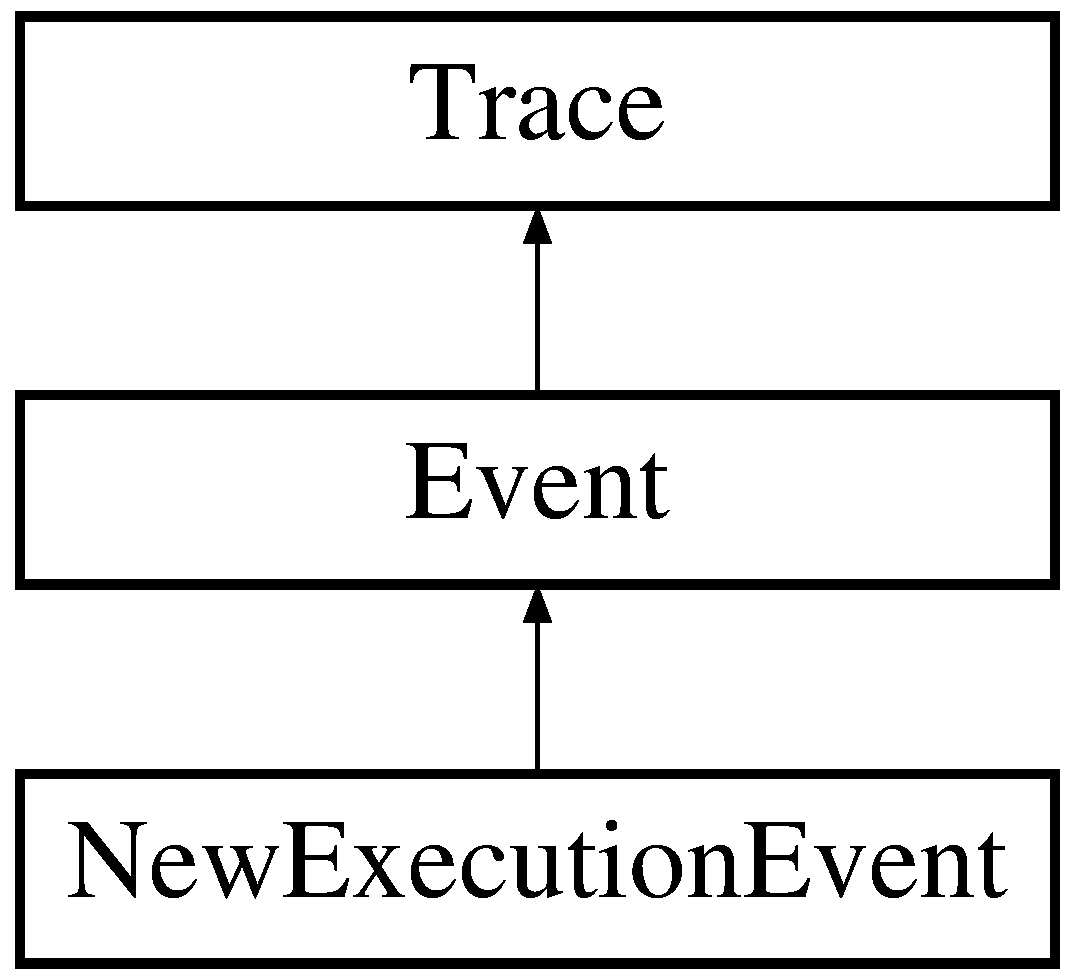
\includegraphics[height=3.000000cm]{class_new_execution_event}
\end{center}
\end{figure}
\subsection*{Public Member Functions}
\begin{DoxyCompactItemize}
\item 
\hyperlink{class_new_execution_event_ae957f1481d67e50e6816b38c03debecf}{New\+Execution\+Event} (int start\+\_\+time)
\item 
\hyperlink{class_new_execution_event_a84fae0b583bd7692a70c34ead8f19e50}{New\+Execution\+Event} (const \hyperlink{class_new_execution_event}{New\+Execution\+Event} $\ast$nee)
\item 
virtual \hyperlink{class_trace_a9c58e523529fc8a03fb6acf3eef86150}{Trace\+::sp\+\_\+trace} \hyperlink{class_new_execution_event_adc75351c4c45e5161c26138b29e980ed}{clone} () const 
\begin{DoxyCompactList}\small\item\em Clonage d\textquotesingle{}un événement. \end{DoxyCompactList}\item 
virtual std\+::string \hyperlink{class_new_execution_event_a1d28826bae4c7b73bc85859f62f48a48}{get\+Params} () const 
\begin{DoxyCompactList}\small\item\em Retourne les différents paramètres relatifs à l\textquotesingle{}événement sous forme de chaîne de caractères. \end{DoxyCompactList}\item 
int \hyperlink{class_new_execution_event_a677aa6cf9f100dd4522b6e467c264030}{get\+Start\+Time} () const 
\end{DoxyCompactItemize}
\subsection*{Additional Inherited Members}


\subsection{Detailed Description}


Definition at line 81 of file Event\+Def.\+h.



\subsection{Constructor \& Destructor Documentation}
\index{New\+Execution\+Event@{New\+Execution\+Event}!New\+Execution\+Event@{New\+Execution\+Event}}
\index{New\+Execution\+Event@{New\+Execution\+Event}!New\+Execution\+Event@{New\+Execution\+Event}}
\subsubsection[{\texorpdfstring{New\+Execution\+Event(int start\+\_\+time)}{NewExecutionEvent(int start_time)}}]{\setlength{\rightskip}{0pt plus 5cm}New\+Execution\+Event\+::\+New\+Execution\+Event (
\begin{DoxyParamCaption}
\item[{int}]{start\+\_\+time}
\end{DoxyParamCaption}
)\hspace{0.3cm}{\ttfamily [inline]}}\hypertarget{class_new_execution_event_ae957f1481d67e50e6816b38c03debecf}{}\label{class_new_execution_event_ae957f1481d67e50e6816b38c03debecf}


Definition at line 85 of file Event\+Def.\+h.

\index{New\+Execution\+Event@{New\+Execution\+Event}!New\+Execution\+Event@{New\+Execution\+Event}}
\index{New\+Execution\+Event@{New\+Execution\+Event}!New\+Execution\+Event@{New\+Execution\+Event}}
\subsubsection[{\texorpdfstring{New\+Execution\+Event(const New\+Execution\+Event $\ast$nee)}{NewExecutionEvent(const NewExecutionEvent *nee)}}]{\setlength{\rightskip}{0pt plus 5cm}New\+Execution\+Event\+::\+New\+Execution\+Event (
\begin{DoxyParamCaption}
\item[{const {\bf New\+Execution\+Event} $\ast$}]{nee}
\end{DoxyParamCaption}
)\hspace{0.3cm}{\ttfamily [inline]}}\hypertarget{class_new_execution_event_a84fae0b583bd7692a70c34ead8f19e50}{}\label{class_new_execution_event_a84fae0b583bd7692a70c34ead8f19e50}


Definition at line 87 of file Event\+Def.\+h.



\subsection{Member Function Documentation}
\index{New\+Execution\+Event@{New\+Execution\+Event}!clone@{clone}}
\index{clone@{clone}!New\+Execution\+Event@{New\+Execution\+Event}}
\subsubsection[{\texorpdfstring{clone() const }{clone() const }}]{\setlength{\rightskip}{0pt plus 5cm}virtual {\bf Trace\+::sp\+\_\+trace} New\+Execution\+Event\+::clone (
\begin{DoxyParamCaption}
{}
\end{DoxyParamCaption}
) const\hspace{0.3cm}{\ttfamily [inline]}, {\ttfamily [virtual]}}\hypertarget{class_new_execution_event_adc75351c4c45e5161c26138b29e980ed}{}\label{class_new_execution_event_adc75351c4c45e5161c26138b29e980ed}


Clonage d\textquotesingle{}un événement. 

\begin{DoxyReturn}{Returns}
une copie de l\textquotesingle{}objet \hyperlink{class_event}{Event}. 
\end{DoxyReturn}


Reimplemented from \hyperlink{class_event_aafa2022d6600717a9cd6511797548265}{Event}.



Definition at line 91 of file Event\+Def.\+h.

\index{New\+Execution\+Event@{New\+Execution\+Event}!get\+Params@{get\+Params}}
\index{get\+Params@{get\+Params}!New\+Execution\+Event@{New\+Execution\+Event}}
\subsubsection[{\texorpdfstring{get\+Params() const }{getParams() const }}]{\setlength{\rightskip}{0pt plus 5cm}virtual std\+::string New\+Execution\+Event\+::get\+Params (
\begin{DoxyParamCaption}
{}
\end{DoxyParamCaption}
) const\hspace{0.3cm}{\ttfamily [inline]}, {\ttfamily [virtual]}}\hypertarget{class_new_execution_event_a1d28826bae4c7b73bc85859f62f48a48}{}\label{class_new_execution_event_a1d28826bae4c7b73bc85859f62f48a48}


Retourne les différents paramètres relatifs à l\textquotesingle{}événement sous forme de chaîne de caractères. 

Cette fonction doit être redéfinie par les classes héritant de \hyperlink{class_event}{Event}.

\begin{DoxyReturn}{Returns}
la chaîne de caractères formatée contenant les valeurs des différents paramètres de l\textquotesingle{}événement séparées par des espaces. 
\end{DoxyReturn}


Reimplemented from \hyperlink{class_event_aad213c94070547bb727ba369b3460e2a}{Event}.



Definition at line 95 of file Event\+Def.\+h.

\index{New\+Execution\+Event@{New\+Execution\+Event}!get\+Start\+Time@{get\+Start\+Time}}
\index{get\+Start\+Time@{get\+Start\+Time}!New\+Execution\+Event@{New\+Execution\+Event}}
\subsubsection[{\texorpdfstring{get\+Start\+Time() const }{getStartTime() const }}]{\setlength{\rightskip}{0pt plus 5cm}int New\+Execution\+Event\+::get\+Start\+Time (
\begin{DoxyParamCaption}
{}
\end{DoxyParamCaption}
) const\hspace{0.3cm}{\ttfamily [inline]}}\hypertarget{class_new_execution_event_a677aa6cf9f100dd4522b6e467c264030}{}\label{class_new_execution_event_a677aa6cf9f100dd4522b6e467c264030}


Definition at line 99 of file Event\+Def.\+h.



The documentation for this class was generated from the following file\+:\begin{DoxyCompactItemize}
\item 
C\+:/\+Users/\+Stephane/\+Desktop/mocahteam/\+Prog\+And\+Play/pp/traces/src/\hyperlink{_event_def_8h}{Event\+Def.\+h}\end{DoxyCompactItemize}

\hypertarget{class_no_param_call}{}\section{No\+Param\+Call Class Reference}
\label{class_no_param_call}\index{No\+Param\+Call@{No\+Param\+Call}}


{\ttfamily \#include $<$Call\+Def.\+h$>$}

Inheritance diagram for No\+Param\+Call\+:\begin{figure}[H]
\begin{center}
\leavevmode
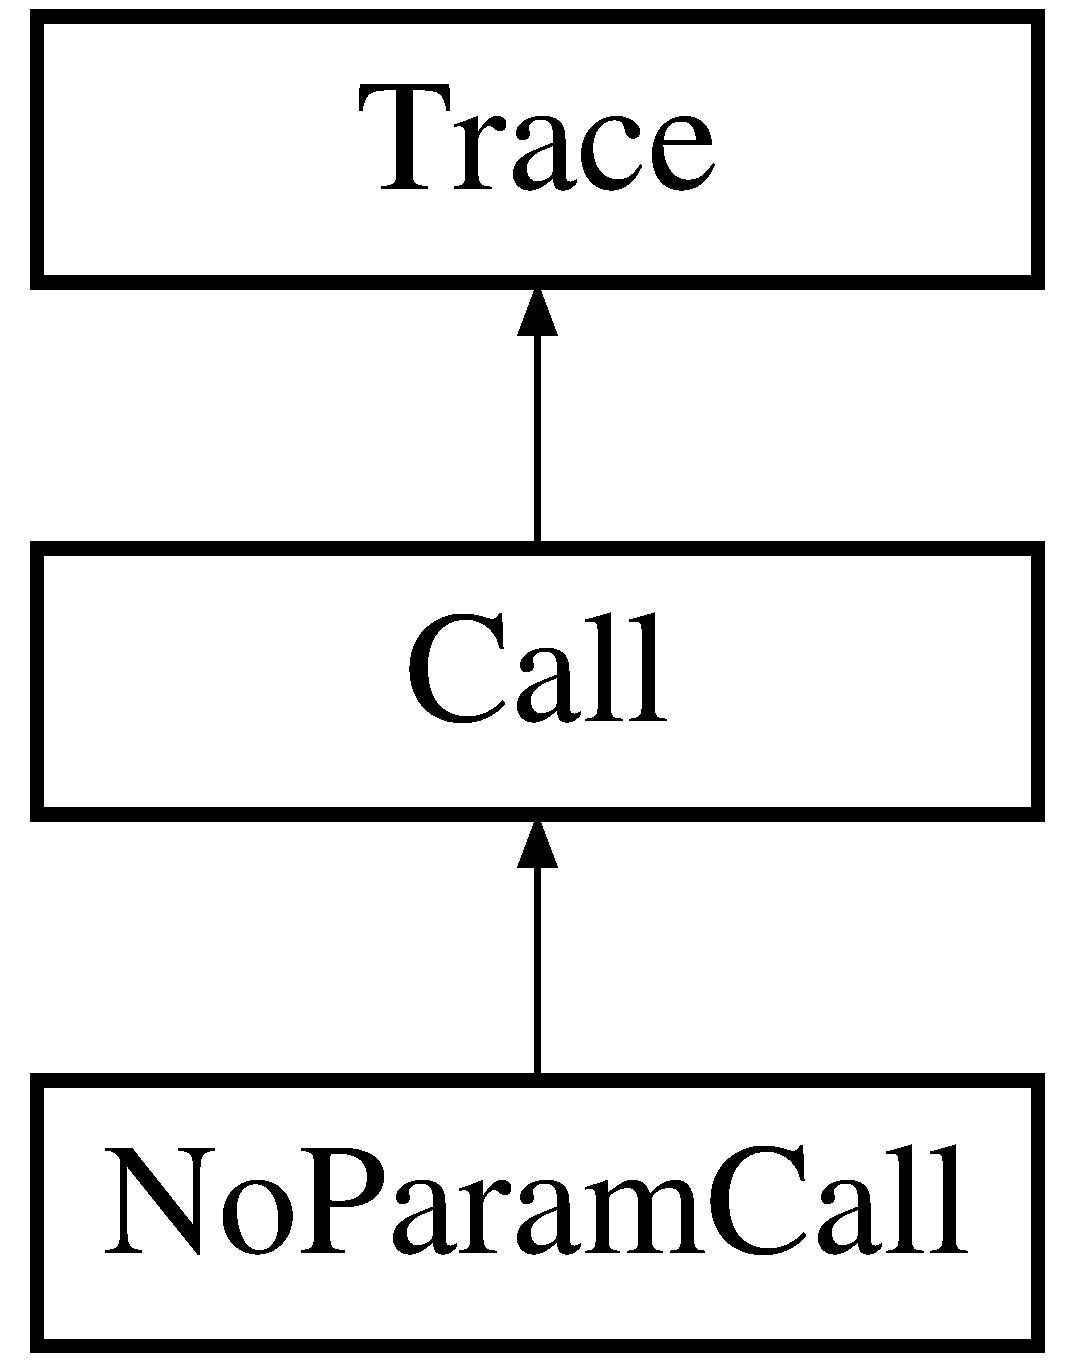
\includegraphics[height=3.000000cm]{class_no_param_call}
\end{center}
\end{figure}
\subsection*{Public Member Functions}
\begin{DoxyCompactItemize}
\item 
\hyperlink{class_no_param_call_a8ddb088ba749768c4fc3df01f0c35fa1}{No\+Param\+Call} (std\+::string \hyperlink{class_call_ad6b8343d530798fdb48407b3f2489ae7}{label})
\item 
\hyperlink{class_no_param_call_ae4e6dcc8a8705c578cac1acc045c7886}{No\+Param\+Call} (const \hyperlink{class_no_param_call}{No\+Param\+Call} $\ast$c)
\item 
virtual \hyperlink{class_trace_a9c58e523529fc8a03fb6acf3eef86150}{Trace\+::sp\+\_\+trace} \hyperlink{class_no_param_call_a8488a6947c974711af12b10f89298bf8}{clone} () const 
\begin{DoxyCompactList}\small\item\em Clonage d\textquotesingle{}un appel. \end{DoxyCompactList}\end{DoxyCompactItemize}
\subsection*{Additional Inherited Members}


\subsection{Detailed Description}


Definition at line 46 of file Call\+Def.\+h.



\subsection{Constructor \& Destructor Documentation}
\index{No\+Param\+Call@{No\+Param\+Call}!No\+Param\+Call@{No\+Param\+Call}}
\index{No\+Param\+Call@{No\+Param\+Call}!No\+Param\+Call@{No\+Param\+Call}}
\subsubsection[{\texorpdfstring{No\+Param\+Call(std\+::string label)}{NoParamCall(std::string label)}}]{\setlength{\rightskip}{0pt plus 5cm}No\+Param\+Call\+::\+No\+Param\+Call (
\begin{DoxyParamCaption}
\item[{std\+::string}]{label}
\end{DoxyParamCaption}
)\hspace{0.3cm}{\ttfamily [inline]}}\hypertarget{class_no_param_call_a8ddb088ba749768c4fc3df01f0c35fa1}{}\label{class_no_param_call_a8ddb088ba749768c4fc3df01f0c35fa1}


Definition at line 50 of file Call\+Def.\+h.

\index{No\+Param\+Call@{No\+Param\+Call}!No\+Param\+Call@{No\+Param\+Call}}
\index{No\+Param\+Call@{No\+Param\+Call}!No\+Param\+Call@{No\+Param\+Call}}
\subsubsection[{\texorpdfstring{No\+Param\+Call(const No\+Param\+Call $\ast$c)}{NoParamCall(const NoParamCall *c)}}]{\setlength{\rightskip}{0pt plus 5cm}No\+Param\+Call\+::\+No\+Param\+Call (
\begin{DoxyParamCaption}
\item[{const {\bf No\+Param\+Call} $\ast$}]{c}
\end{DoxyParamCaption}
)\hspace{0.3cm}{\ttfamily [inline]}}\hypertarget{class_no_param_call_ae4e6dcc8a8705c578cac1acc045c7886}{}\label{class_no_param_call_ae4e6dcc8a8705c578cac1acc045c7886}


Definition at line 52 of file Call\+Def.\+h.



\subsection{Member Function Documentation}
\index{No\+Param\+Call@{No\+Param\+Call}!clone@{clone}}
\index{clone@{clone}!No\+Param\+Call@{No\+Param\+Call}}
\subsubsection[{\texorpdfstring{clone() const }{clone() const }}]{\setlength{\rightskip}{0pt plus 5cm}virtual {\bf Trace\+::sp\+\_\+trace} No\+Param\+Call\+::clone (
\begin{DoxyParamCaption}
{}
\end{DoxyParamCaption}
) const\hspace{0.3cm}{\ttfamily [inline]}, {\ttfamily [virtual]}}\hypertarget{class_no_param_call_a8488a6947c974711af12b10f89298bf8}{}\label{class_no_param_call_a8488a6947c974711af12b10f89298bf8}


Clonage d\textquotesingle{}un appel. 

\begin{DoxyReturn}{Returns}
une copie de l\textquotesingle{}objet \hyperlink{class_call}{Call}. 
\end{DoxyReturn}


Implements \hyperlink{class_call_ab3bf0965d35eb1e97ecddaf2d3978e9b}{Call}.



Definition at line 54 of file Call\+Def.\+h.



The documentation for this class was generated from the following file\+:\begin{DoxyCompactItemize}
\item 
C\+:/\+Users/\+Stephane/\+Desktop/mocahteam/\+Prog\+And\+Play/pp/traces/src/\hyperlink{_call_def_8h}{Call\+Def.\+h}\end{DoxyCompactItemize}

\hypertarget{class_params_map}{}\section{Params\+Map Class Reference}
\label{class_params_map}\index{Params\+Map@{Params\+Map}}


Classe utilisée pour le chargement des paramètres de compression à partir du fichier J\+S\+ON \textquotesingle{}params.\+json\textquotesingle{}.  




{\ttfamily \#include $<$Call.\+h$>$}

\subsection*{Public Member Functions}
\begin{DoxyCompactItemize}
\item 
\hyperlink{class_params_map_a8d606a7d84a804e9480dbbc1806b29df}{Params\+Map} ()
\begin{DoxyCompactList}\small\item\em Constructeur de la classe \hyperlink{class_params_map}{Params\+Map}. \end{DoxyCompactList}\item 
void \hyperlink{class_params_map_a41a00ad45b0153fa04b35ea474e00786}{init\+Map} (const std\+::string \&json)
\begin{DoxyCompactList}\small\item\em Chargement des paramètres de compression. \end{DoxyCompactList}\item 
bool \hyperlink{class_params_map_af25b9a05c7a95b7d8ff1386014b23e41}{contains} (std\+::string label, std\+::string param) const 
\begin{DoxyCompactList}\small\item\em Récupération des paramètres de compression. \end{DoxyCompactList}\end{DoxyCompactItemize}


\subsection{Detailed Description}
Classe utilisée pour le chargement des paramètres de compression à partir du fichier J\+S\+ON \textquotesingle{}params.\+json\textquotesingle{}. 

Definition at line 34 of file Call.\+h.



\subsection{Constructor \& Destructor Documentation}
\index{Params\+Map@{Params\+Map}!Params\+Map@{Params\+Map}}
\index{Params\+Map@{Params\+Map}!Params\+Map@{Params\+Map}}
\subsubsection[{\texorpdfstring{Params\+Map()}{ParamsMap()}}]{\setlength{\rightskip}{0pt plus 5cm}Params\+Map\+::\+Params\+Map (
\begin{DoxyParamCaption}
{}
\end{DoxyParamCaption}
)\hspace{0.3cm}{\ttfamily [inline]}}\hypertarget{class_params_map_a8d606a7d84a804e9480dbbc1806b29df}{}\label{class_params_map_a8d606a7d84a804e9480dbbc1806b29df}


Constructeur de la classe \hyperlink{class_params_map}{Params\+Map}. 



Definition at line 41 of file Call.\+h.



\subsection{Member Function Documentation}
\index{Params\+Map@{Params\+Map}!contains@{contains}}
\index{contains@{contains}!Params\+Map@{Params\+Map}}
\subsubsection[{\texorpdfstring{contains(std\+::string label, std\+::string param) const }{contains(std::string label, std::string param) const }}]{\setlength{\rightskip}{0pt plus 5cm}bool Params\+Map\+::contains (
\begin{DoxyParamCaption}
\item[{std\+::string}]{label, }
\item[{std\+::string}]{param}
\end{DoxyParamCaption}
) const\hspace{0.3cm}{\ttfamily [inline]}}\hypertarget{class_params_map_af25b9a05c7a95b7d8ff1386014b23e41}{}\label{class_params_map_af25b9a05c7a95b7d8ff1386014b23e41}


Récupération des paramètres de compression. 

Le booléen {\ttfamily loaded} est mis à vrai si la chaine à bien été parsée, de sorte que le chargement ne puisse être effectué qu\textquotesingle{}une seule fois.

Si cette fonction alors que {\ttfamily loaded} est à faux (la fonction \hyperlink{class_params_map_a41a00ad45b0153fa04b35ea474e00786}{Params\+Map\+::init\+Map} n\textquotesingle{}a pas été appelée ou le parsing a échoué), un mode de compression par défaut est utilisé. Suivant la valeur de D\+E\+F\+A\+U\+L\+T\+\_\+\+C\+O\+M\+P\+R\+E\+S\+S\+I\+O\+N\+\_\+\+M\+OD \+:
\begin{DoxyItemize}
\item 0 \+: Aucun paramètre n\textquotesingle{}est pris en considération pour la compression (compression maximale)
\item 1 \+: Tous les paramètres sont pris en considération pour la compression (compression minimale)
\end{DoxyItemize}


\begin{DoxyParams}{Parameters}
{\em label} & \+: un label de fonction utilisée pouvant être utilisée dans \hyperlink{class_call}{Call}. \\
\hline
{\em param} & \+: un nom de paramètre associé à la fonction {\ttfamily label}.\\
\hline
\end{DoxyParams}
\begin{DoxyReturn}{Returns}
vrai si la valeur du paramètre {\ttfamily param} du label {\ttfamily label} doit être pris en considération lors de la compression et faux sinon. 
\end{DoxyReturn}


Definition at line 89 of file Call.\+h.

\index{Params\+Map@{Params\+Map}!init\+Map@{init\+Map}}
\index{init\+Map@{init\+Map}!Params\+Map@{Params\+Map}}
\subsubsection[{\texorpdfstring{init\+Map(const std\+::string \&json)}{initMap(const std::string &json)}}]{\setlength{\rightskip}{0pt plus 5cm}void Params\+Map\+::init\+Map (
\begin{DoxyParamCaption}
\item[{const std\+::string \&}]{json}
\end{DoxyParamCaption}
)\hspace{0.3cm}{\ttfamily [inline]}}\hypertarget{class_params_map_a41a00ad45b0153fa04b35ea474e00786}{}\label{class_params_map_a41a00ad45b0153fa04b35ea474e00786}


Chargement des paramètres de compression. 

Le booléen {\ttfamily loaded} est mis à vrai si la chaine à bien été parsée, de sorte que le chargement ne puisse être effectué qu\textquotesingle{}une seule fois.


\begin{DoxyParams}{Parameters}
{\em json} & \+: une chaîne de caractères contenant les données au format J\+S\+ON. \\
\hline
\end{DoxyParams}


Definition at line 50 of file Call.\+h.



The documentation for this class was generated from the following file\+:\begin{DoxyCompactItemize}
\item 
C\+:/\+Users/\+Stephane/\+Desktop/mocahteam/\+Prog\+And\+Play/pp/traces/src/\hyperlink{_call_8h}{Call.\+h}\end{DoxyCompactItemize}

\hypertarget{struct_call_misc_1_1_position}{}\section{Call\+Misc\+:\+:Position Struct Reference}
\label{struct_call_misc_1_1_position}\index{Call\+Misc\+::\+Position@{Call\+Misc\+::\+Position}}


{\ttfamily \#include $<$Call\+Def.\+h$>$}

\subsection*{Public Member Functions}
\begin{DoxyCompactItemize}
\item 
bool \hyperlink{struct_call_misc_1_1_position_a5fac3deeb3167aaee5ced59395b58c36}{operator!=} (const \hyperlink{struct_call_misc_1_1_position}{Position} \&p) const 
\end{DoxyCompactItemize}
\subsection*{Public Attributes}
\begin{DoxyCompactItemize}
\item 
float \hyperlink{struct_call_misc_1_1_position_a4ba3eeb200b5d953be679bffe632c987}{x}
\item 
float \hyperlink{struct_call_misc_1_1_position_ae9515216882a99805c4b2b62c75cc1be}{y}
\end{DoxyCompactItemize}


\subsection{Detailed Description}


Definition at line 35 of file Call\+Def.\+h.



\subsection{Member Function Documentation}
\index{Call\+Misc\+::\+Position@{Call\+Misc\+::\+Position}!operator"!=@{operator"!=}}
\index{operator"!=@{operator"!=}!Call\+Misc\+::\+Position@{Call\+Misc\+::\+Position}}
\subsubsection[{\texorpdfstring{operator"!=(const Position \&p) const }{operator!=(const Position &p) const }}]{\setlength{\rightskip}{0pt plus 5cm}bool Call\+Misc\+::\+Position\+::operator!= (
\begin{DoxyParamCaption}
\item[{const {\bf Position} \&}]{p}
\end{DoxyParamCaption}
) const\hspace{0.3cm}{\ttfamily [inline]}}\hypertarget{struct_call_misc_1_1_position_a5fac3deeb3167aaee5ced59395b58c36}{}\label{struct_call_misc_1_1_position_a5fac3deeb3167aaee5ced59395b58c36}


Definition at line 39 of file Call\+Def.\+h.



\subsection{Member Data Documentation}
\index{Call\+Misc\+::\+Position@{Call\+Misc\+::\+Position}!x@{x}}
\index{x@{x}!Call\+Misc\+::\+Position@{Call\+Misc\+::\+Position}}
\subsubsection[{\texorpdfstring{x}{x}}]{\setlength{\rightskip}{0pt plus 5cm}float Call\+Misc\+::\+Position\+::x}\hypertarget{struct_call_misc_1_1_position_a4ba3eeb200b5d953be679bffe632c987}{}\label{struct_call_misc_1_1_position_a4ba3eeb200b5d953be679bffe632c987}


Definition at line 36 of file Call\+Def.\+h.

\index{Call\+Misc\+::\+Position@{Call\+Misc\+::\+Position}!y@{y}}
\index{y@{y}!Call\+Misc\+::\+Position@{Call\+Misc\+::\+Position}}
\subsubsection[{\texorpdfstring{y}{y}}]{\setlength{\rightskip}{0pt plus 5cm}float Call\+Misc\+::\+Position\+::y}\hypertarget{struct_call_misc_1_1_position_ae9515216882a99805c4b2b62c75cc1be}{}\label{struct_call_misc_1_1_position_ae9515216882a99805c4b2b62c75cc1be}


Definition at line 37 of file Call\+Def.\+h.



The documentation for this struct was generated from the following file\+:\begin{DoxyCompactItemize}
\item 
C\+:/\+Users/\+Stephane/\+Desktop/mocahteam/\+Prog\+And\+Play/pp/traces/src/\hyperlink{_call_def_8h}{Call\+Def.\+h}\end{DoxyCompactItemize}

\hypertarget{class_sequence}{}\section{Sequence Class Reference}
\label{class_sequence}\index{Sequence@{Sequence}}


La classe \hyperlink{class_sequence}{Sequence} hérite de la classe.  




{\ttfamily \#include $<$Sequence.\+h$>$}

Inheritance diagram for Sequence\+:\begin{figure}[H]
\begin{center}
\leavevmode
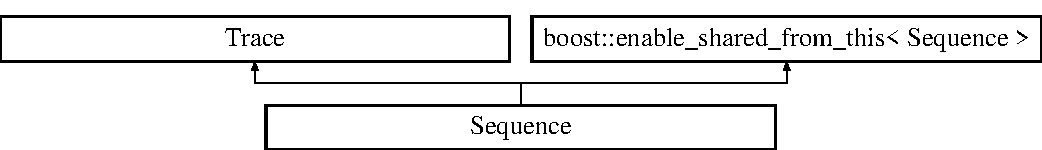
\includegraphics[height=2.000000cm]{class_sequence}
\end{center}
\end{figure}
\subsection*{Public Types}
\begin{DoxyCompactItemize}
\item 
typedef boost\+::shared\+\_\+ptr$<$ \hyperlink{class_sequence}{Sequence} $>$ \hyperlink{class_sequence_a796bfa70aa4ddd4e447c210655b5dc5a}{sp\+\_\+sequence}
\item 
typedef boost\+::shared\+\_\+ptr$<$ const \hyperlink{class_sequence}{Sequence} $>$ \hyperlink{class_sequence_ad2a8856e4c26f405a86b0cb9683c25ed}{const\+\_\+sp\+\_\+sequence}
\item 
typedef std\+::vector$<$ \hyperlink{class_sequence_a796bfa70aa4ddd4e447c210655b5dc5a}{sp\+\_\+sequence} $>$ \hyperlink{class_sequence_a4487def8096371d361c6099c2d46dd13}{sequence\+\_\+vector}
\end{DoxyCompactItemize}
\subsection*{Public Member Functions}
\begin{DoxyCompactItemize}
\item 
\hyperlink{class_sequence_a6005e244485149e7daa5650f0bd29186}{Sequence} (std\+::string \hyperlink{class_trace_a4835dcfa7da5d4c971e8f7d6860acb09}{info}, bool \hyperlink{class_sequence_ae495f3d3267ac936660920ab13b2316e}{num\+\_\+fixed})
\begin{DoxyCompactList}\small\item\em Constructeur utilisé dans la fonction \hyperlink{class_traces_parser_a515973e07e60b36499649239592f6edb}{Traces\+Parser\+::import\+Trace\+From\+Node}. \end{DoxyCompactList}\item 
\hyperlink{class_sequence_a1d61d80db0f83560c70880673c5186a0}{Sequence} (unsigned int \hyperlink{class_sequence_a9283bd1da021b06eeaed1028b1e7069e}{num}, bool \hyperlink{class_sequence_ac09da762e43cc657842d4f953ffff613}{root}=false)
\begin{DoxyCompactList}\small\item\em Constructeur principal de la classe \hyperlink{class_sequence}{Sequence}. \end{DoxyCompactList}\item 
\hyperlink{class_sequence_a2c6d8767415f842e22c68008225d7c22}{Sequence} (\hyperlink{class_sequence_ad2a8856e4c26f405a86b0cb9683c25ed}{const\+\_\+sp\+\_\+sequence} sps)
\begin{DoxyCompactList}\small\item\em Constructeur se basant sur une séquence. \end{DoxyCompactList}\item 
\hyperlink{class_sequence_ae5975e693da40545b8326a9d3f33229a}{Sequence} (\hyperlink{class_sequence_ad2a8856e4c26f405a86b0cb9683c25ed}{const\+\_\+sp\+\_\+sequence} sps\+\_\+up, \hyperlink{class_sequence_ad2a8856e4c26f405a86b0cb9683c25ed}{const\+\_\+sp\+\_\+sequence} sps\+\_\+down)
\begin{DoxyCompactList}\small\item\em Constructeur se basant sur deux séquences. \end{DoxyCompactList}\item 
virtual unsigned int \hyperlink{class_sequence_a6da226d77ff5150ced893f0b6c83f83a}{length} () const 
\begin{DoxyCompactList}\small\item\em Récupération de la longueur (l\textquotesingle{}espace occupé dans un vecteur de traces) d\textquotesingle{}une séquence. \end{DoxyCompactList}\item 
virtual bool \hyperlink{class_sequence_a945e1cb29fadc554bc8a3d61f188998c}{operator==} (\hyperlink{class_trace}{Trace} $\ast$t) const 
\begin{DoxyCompactList}\small\item\em Comparaison de la séquence avec une trace. \end{DoxyCompactList}\item 
virtual \hyperlink{class_trace_a9c58e523529fc8a03fb6acf3eef86150}{Trace\+::sp\+\_\+trace} \hyperlink{class_sequence_aad8c31973496749c3e57848af2812284}{clone} () const 
\begin{DoxyCompactList}\small\item\em Clonage d\textquotesingle{}une séquence. \end{DoxyCompactList}\item 
virtual void \hyperlink{class_sequence_a19d7d6f49253cbaae84cc802760c7d38}{display} (std\+::ostream \&os=std\+::cout) const 
\begin{DoxyCompactList}\small\item\em Affichage des informations de l\textquotesingle{}objet \hyperlink{class_sequence}{Sequence}. \end{DoxyCompactList}\item 
virtual void \hyperlink{class_sequence_aacd81267429077588208d2a040ea51e4}{reset\+Aligned} ()
\begin{DoxyCompactList}\small\item\em Réinitialisation récursive de l\textquotesingle{}alignement de la séquence. \end{DoxyCompactList}\item 
bool \hyperlink{class_sequence_a1d6dedda9e2b8bb5489a7cca5e21a220}{compare} (\hyperlink{class_trace}{Trace} $\ast$t)
\begin{DoxyCompactList}\small\item\em Comparaison de la séquence avec une trace. \end{DoxyCompactList}\item 
std\+::vector$<$ \hyperlink{class_trace_a9c58e523529fc8a03fb6acf3eef86150}{Trace\+::sp\+\_\+trace} $>$ \& \hyperlink{class_sequence_a4d3e82279c084b43f99171b6dc2ad4eb}{get\+Traces} ()
\begin{DoxyCompactList}\small\item\em Getter pour le vecteur de traces de la séquence \hyperlink{class_sequence_a2e22b6d3eda29911dda95aa36efefa83}{Sequence\+::traces}. \end{DoxyCompactList}\item 
unsigned int \hyperlink{class_sequence_af33fa151c98bbf84a28823cd09ee7d9a}{get\+Pt} () const 
\begin{DoxyCompactList}\small\item\em Getter pour la variable \hyperlink{class_sequence_a6005aee7fd142d6292dcfeefe062bc82}{Sequence\+::pt}. \end{DoxyCompactList}\item 
unsigned int \hyperlink{class_sequence_a4cc3d5e3e7d3f289e920aa3e5c9e92ee}{get\+Num} () const 
\begin{DoxyCompactList}\small\item\em Getter pour la variable \hyperlink{class_sequence_a9283bd1da021b06eeaed1028b1e7069e}{Sequence\+::num}. \end{DoxyCompactList}\item 
const std\+::map$<$ unsigned int, unsigned int $>$ \& \hyperlink{class_sequence_abb5f09294c5e976997d1a8350b4d2996}{get\+Num\+Map} () const 
\begin{DoxyCompactList}\small\item\em Getter pour la variable \hyperlink{class_sequence_a3fb6b6543259ea07c976012dd622cdcc}{Sequence\+::num\+Map}. \end{DoxyCompactList}\item 
bool \hyperlink{class_sequence_a32de7afc9fdde5cdacc5ea445b3dd4d3}{has\+Number\+Iteration\+Fixed} () const 
\begin{DoxyCompactList}\small\item\em Getter pour la variable \hyperlink{class_sequence_ae495f3d3267ac936660920ab13b2316e}{Sequence\+::num\+\_\+fixed}. \end{DoxyCompactList}\item 
bool \hyperlink{class_sequence_a294b1ccae843cd2e5da5e240688b514b}{is\+End\+Reached} () const 
\begin{DoxyCompactList}\small\item\em Getter pour la variable \hyperlink{class_sequence_a37ae535e71d53216a85e16bec941410d}{Sequence\+::end\+Reached}. \end{DoxyCompactList}\item 
bool \hyperlink{class_sequence_a7687abf7372c74369a1e892127c3c3fa}{is\+Shared} () const 
\begin{DoxyCompactList}\small\item\em Getter pour la variable \hyperlink{class_sequence_a77c5ea96e0222cb80d5a8cf420e1d624}{Sequence\+::shared}. \end{DoxyCompactList}\item 
bool \hyperlink{class_sequence_a231764f7959252b2c95e7658c5c1fd19}{is\+Root} () const 
\begin{DoxyCompactList}\small\item\em Getter pour la variable \hyperlink{class_sequence_ac09da762e43cc657842d4f953ffff613}{Sequence\+::root}. \end{DoxyCompactList}\item 
bool \hyperlink{class_sequence_a0eee9fda2394b83b440911f4fc888b60}{is\+Implicit} () const 
\begin{DoxyCompactList}\small\item\em Test si la séquence est une séquence implicite. \end{DoxyCompactList}\item 
unsigned int \hyperlink{class_sequence_a40b394b58ce0a47d2e265f098eb8edca}{size} () const 
\begin{DoxyCompactList}\small\item\em Taille du vecteur de traces de la séquence. \end{DoxyCompactList}\item 
const \hyperlink{class_trace_a9c58e523529fc8a03fb6acf3eef86150}{Trace\+::sp\+\_\+trace} \& \hyperlink{class_sequence_a65030d6b4be29f3747f646d2b246c05c}{at} (unsigned int i) const 
\begin{DoxyCompactList}\small\item\em Accès à une trace du vecteur de traces de la séquence. \end{DoxyCompactList}\item 
int \hyperlink{class_sequence_ac312884c78445acddcdb9d96a6a3b4b7}{get\+Index} (const \hyperlink{class_trace_a9c58e523529fc8a03fb6acf3eef86150}{Trace\+::sp\+\_\+trace} \&spt) const 
\begin{DoxyCompactList}\small\item\em Récupération de l\textquotesingle{}indice de la position d\textquotesingle{}une trace dans le vecteur de traces de la séquence. \end{DoxyCompactList}\item 
\hyperlink{class_call_aa446a4316c03fb722ab10d0e1da33643}{Call\+::call\+\_\+vector} \hyperlink{class_sequence_ae19d30e099accaf9dd07b21d434c67e2}{get\+Calls} (bool set\+Mod=false)
\begin{DoxyCompactList}\small\item\em Récupération de l\textquotesingle{}ensemble des appels contenus dans la séquence et dans ses sous-\/séquences. \end{DoxyCompactList}\item 
\hyperlink{class_sequence_a4487def8096371d361c6099c2d46dd13}{sequence\+\_\+vector} \hyperlink{class_sequence_a066802ba99f1fd93fff062d1b54ca985}{get\+Sequences} ()
\begin{DoxyCompactList}\small\item\em Récupération de l\textquotesingle{}ensemble des séquences contenues dans la séquence et dans ses sous-\/séquences. \end{DoxyCompactList}\item 
void \hyperlink{class_sequence_a901736e6e3f64dcb3a4c12892bc5dc92}{add\+One} ()
\begin{DoxyCompactList}\small\item\em Ajout d\textquotesingle{}une répétition pour la séquence. \end{DoxyCompactList}\item 
bool \hyperlink{class_sequence_a74e000d0651eb8d4c7bfd20032440c07}{add\+Trace} (\hyperlink{class_trace_a9c58e523529fc8a03fb6acf3eef86150}{Trace\+::sp\+\_\+trace} spt, int ind=-\/1)
\begin{DoxyCompactList}\small\item\em Ajout d\textquotesingle{}une trace dans le vecteur de la séquence. \end{DoxyCompactList}\item 
const \hyperlink{class_trace_a9c58e523529fc8a03fb6acf3eef86150}{Trace\+::sp\+\_\+trace} \& \hyperlink{class_sequence_a5c6f4d1232eb3fddc256a2d654c48c6b}{next} ()
\begin{DoxyCompactList}\small\item\em Récupération de la prochaine trace dans le vecteur de la séquence. \end{DoxyCompactList}\item 
void \hyperlink{class_sequence_af1dbfa6630d8224407b489658f3cae13}{reset} ()
\begin{DoxyCompactList}\small\item\em Réinitialisation du parcours de la séquence. \end{DoxyCompactList}\item 
bool \hyperlink{class_sequence_a4332a20962a5bda02bba87789c06490d}{check\+Delayed} ()
\begin{DoxyCompactList}\small\item\em Test si le champ \hyperlink{class_trace_a9757057cc65f9e45bbeaa848cb06d5a1}{Trace\+::delayed} de la séquence doit être mis à vrai. \end{DoxyCompactList}\item 
void \hyperlink{class_sequence_a3cbca7f0a868e768d112e61f2087cbae}{update\+Num\+Map} (unsigned int \hyperlink{class_sequence_a9283bd1da021b06eeaed1028b1e7069e}{num}, int update=1)
\begin{DoxyCompactList}\small\item\em Mise à jour de \hyperlink{class_sequence_a3fb6b6543259ea07c976012dd622cdcc}{Sequence\+::num\+Map}. \end{DoxyCompactList}\item 
void \hyperlink{class_sequence_a03ef5cb5c25d9a9de0f5c61d786580bb}{update\+Num\+Map} (const std\+::map$<$ unsigned int, unsigned int $>$ \&\hyperlink{class_sequence_a3fb6b6543259ea07c976012dd622cdcc}{num\+Map})
\begin{DoxyCompactList}\small\item\em Mise à jour de \hyperlink{class_sequence_a3fb6b6543259ea07c976012dd622cdcc}{Sequence\+::num\+Map} à partir d\textquotesingle{}une autre \hyperlink{class_sequence_a3fb6b6543259ea07c976012dd622cdcc}{Sequence\+::num\+Map}. \end{DoxyCompactList}\item 
void \hyperlink{class_sequence_a2069ef17dde51540555a4aada06977fb}{complete\+Num\+Map} ()
\begin{DoxyCompactList}\small\item\em Complétion de \hyperlink{class_sequence_a3fb6b6543259ea07c976012dd622cdcc}{Sequence\+::num\+Map}. \end{DoxyCompactList}\item 
std\+::map$<$ unsigned int, double $>$ \hyperlink{class_sequence_aa2f856b4cbc1aa775824144caa4d47e3}{get\+Percentage\+Num\+Map} () const 
\begin{DoxyCompactList}\small\item\em Récupération des fréquences de répétitions de la séquence. \end{DoxyCompactList}\item 
double \hyperlink{class_sequence_aa619292ed4984e6f7f4f3010caa55d16}{get\+Num\+Map\+Mean\+Distance} (const \hyperlink{class_sequence_a796bfa70aa4ddd4e447c210655b5dc5a}{sp\+\_\+sequence} \&sps) const 
\begin{DoxyCompactList}\small\item\em Calcul de la distance entre deux objets \hyperlink{class_sequence_a3fb6b6543259ea07c976012dd622cdcc}{Sequence\+::num\+Map}. \end{DoxyCompactList}\end{DoxyCompactItemize}
\subsection*{Static Public Member Functions}
\begin{DoxyCompactItemize}
\item 
{\footnotesize template$<$typename T $>$ }\\static std\+::string \hyperlink{class_sequence_a161ac4fab17750ca48b1fe5053bc1c98}{get\+Num\+Map\+String} (const std\+::map$<$ unsigned int, T $>$ \&\hyperlink{class_sequence_a3fb6b6543259ea07c976012dd622cdcc}{num\+Map})
\begin{DoxyCompactList}\small\item\em Construction d\textquotesingle{}une chaîne de caractères contenant les entrées d\textquotesingle{}un objet \hyperlink{class_sequence_a3fb6b6543259ea07c976012dd622cdcc}{Sequence\+::num\+Map}. \end{DoxyCompactList}\end{DoxyCompactItemize}
\subsection*{Protected Attributes}
\begin{DoxyCompactItemize}
\item 
bool \hyperlink{class_sequence_ae495f3d3267ac936660920ab13b2316e}{num\+\_\+fixed}
\item 
std\+::vector$<$ \hyperlink{class_trace_a9c58e523529fc8a03fb6acf3eef86150}{Trace\+::sp\+\_\+trace} $>$ \hyperlink{class_sequence_a2e22b6d3eda29911dda95aa36efefa83}{traces}
\item 
unsigned int \hyperlink{class_sequence_a9283bd1da021b06eeaed1028b1e7069e}{num}
\item 
std\+::map$<$ unsigned int, unsigned int $>$ \hyperlink{class_sequence_a3fb6b6543259ea07c976012dd622cdcc}{num\+Map}
\item 
unsigned int \hyperlink{class_sequence_a6005aee7fd142d6292dcfeefe062bc82}{pt}
\item 
bool \hyperlink{class_sequence_a37ae535e71d53216a85e16bec941410d}{end\+Reached}
\item 
bool \hyperlink{class_sequence_a77c5ea96e0222cb80d5a8cf420e1d624}{shared}
\item 
bool \hyperlink{class_sequence_ac09da762e43cc657842d4f953ffff613}{root}
\end{DoxyCompactItemize}
\subsection*{Additional Inherited Members}


\subsection{Detailed Description}
La classe \hyperlink{class_sequence}{Sequence} hérite de la classe. 

\begin{DoxySeeAlso}{See also}
\hyperlink{class_trace}{Trace}. Une séquence possède un vecteur d\textquotesingle{}objets \hyperlink{class_trace}{Trace}. 
\end{DoxySeeAlso}


Definition at line 28 of file Sequence.\+h.



\subsection{Member Typedef Documentation}
\index{Sequence@{Sequence}!const\+\_\+sp\+\_\+sequence@{const\+\_\+sp\+\_\+sequence}}
\index{const\+\_\+sp\+\_\+sequence@{const\+\_\+sp\+\_\+sequence}!Sequence@{Sequence}}
\subsubsection[{\texorpdfstring{const\+\_\+sp\+\_\+sequence}{const_sp_sequence}}]{\setlength{\rightskip}{0pt plus 5cm}typedef boost\+::shared\+\_\+ptr$<$const {\bf Sequence}$>$ {\bf Sequence\+::const\+\_\+sp\+\_\+sequence}}\hypertarget{class_sequence_ad2a8856e4c26f405a86b0cb9683c25ed}{}\label{class_sequence_ad2a8856e4c26f405a86b0cb9683c25ed}


Definition at line 36 of file Sequence.\+h.

\index{Sequence@{Sequence}!sequence\+\_\+vector@{sequence\+\_\+vector}}
\index{sequence\+\_\+vector@{sequence\+\_\+vector}!Sequence@{Sequence}}
\subsubsection[{\texorpdfstring{sequence\+\_\+vector}{sequence_vector}}]{\setlength{\rightskip}{0pt plus 5cm}typedef std\+::vector$<${\bf sp\+\_\+sequence}$>$ {\bf Sequence\+::sequence\+\_\+vector}}\hypertarget{class_sequence_a4487def8096371d361c6099c2d46dd13}{}\label{class_sequence_a4487def8096371d361c6099c2d46dd13}


Definition at line 37 of file Sequence.\+h.

\index{Sequence@{Sequence}!sp\+\_\+sequence@{sp\+\_\+sequence}}
\index{sp\+\_\+sequence@{sp\+\_\+sequence}!Sequence@{Sequence}}
\subsubsection[{\texorpdfstring{sp\+\_\+sequence}{sp_sequence}}]{\setlength{\rightskip}{0pt plus 5cm}typedef boost\+::shared\+\_\+ptr$<${\bf Sequence}$>$ {\bf Sequence\+::sp\+\_\+sequence}}\hypertarget{class_sequence_a796bfa70aa4ddd4e447c210655b5dc5a}{}\label{class_sequence_a796bfa70aa4ddd4e447c210655b5dc5a}
Définition du type pointeur intelligent vers un objet \hyperlink{class_sequence}{Sequence}. 

Definition at line 35 of file Sequence.\+h.



\subsection{Constructor \& Destructor Documentation}
\index{Sequence@{Sequence}!Sequence@{Sequence}}
\index{Sequence@{Sequence}!Sequence@{Sequence}}
\subsubsection[{\texorpdfstring{Sequence(std\+::string info, bool num\+\_\+fixed)}{Sequence(std::string info, bool num_fixed)}}]{\setlength{\rightskip}{0pt plus 5cm}Sequence\+::\+Sequence (
\begin{DoxyParamCaption}
\item[{std\+::string}]{info, }
\item[{bool}]{num\+\_\+fixed}
\end{DoxyParamCaption}
)}\hypertarget{class_sequence_a6005e244485149e7daa5650f0bd29186}{}\label{class_sequence_a6005e244485149e7daa5650f0bd29186}


Constructeur utilisé dans la fonction \hyperlink{class_traces_parser_a515973e07e60b36499649239592f6edb}{Traces\+Parser\+::import\+Trace\+From\+Node}. 


\begin{DoxyParams}{Parameters}
{\em info} & label de la séquence ajouté par l\textquotesingle{}expert. \\
\hline
{\em num\+\_\+fixed} & valeur de l\textquotesingle{}attribut num\+\_\+fixed indiquée par l\textquotesingle{}expert.\\
\hline
\end{DoxyParams}
\begin{DoxySeeAlso}{See also}
\hyperlink{class_traces_parser_a515973e07e60b36499649239592f6edb}{Traces\+Parser\+::import\+Trace\+From\+Node} 
\end{DoxySeeAlso}


Definition at line 3 of file Sequence.\+cpp.

\index{Sequence@{Sequence}!Sequence@{Sequence}}
\index{Sequence@{Sequence}!Sequence@{Sequence}}
\subsubsection[{\texorpdfstring{Sequence(unsigned int num, bool root=false)}{Sequence(unsigned int num, bool root=false)}}]{\setlength{\rightskip}{0pt plus 5cm}Sequence\+::\+Sequence (
\begin{DoxyParamCaption}
\item[{unsigned int}]{num, }
\item[{bool}]{root = {\ttfamily false}}
\end{DoxyParamCaption}
)}\hypertarget{class_sequence_a1d61d80db0f83560c70880673c5186a0}{}\label{class_sequence_a1d61d80db0f83560c70880673c5186a0}


Constructeur principal de la classe \hyperlink{class_sequence}{Sequence}. 


\begin{DoxyParams}{Parameters}
{\em num} & le nombre de répétitions contiguës de la séquence. \\
\hline
{\em root} & booléen mis à vrai si la séquence créée est une racine. \\
\hline
\end{DoxyParams}


Definition at line 5 of file Sequence.\+cpp.

\index{Sequence@{Sequence}!Sequence@{Sequence}}
\index{Sequence@{Sequence}!Sequence@{Sequence}}
\subsubsection[{\texorpdfstring{Sequence(const\+\_\+sp\+\_\+sequence sps)}{Sequence(const_sp_sequence sps)}}]{\setlength{\rightskip}{0pt plus 5cm}Sequence\+::\+Sequence (
\begin{DoxyParamCaption}
\item[{{\bf const\+\_\+sp\+\_\+sequence}}]{sps}
\end{DoxyParamCaption}
)}\hypertarget{class_sequence_a2c6d8767415f842e22c68008225d7c22}{}\label{class_sequence_a2c6d8767415f842e22c68008225d7c22}


Constructeur se basant sur une séquence. 


\begin{DoxyParams}{Parameters}
{\em sps} & la séquence utilisée pour la construction de la nouvelle séquence. \\
\hline
\end{DoxyParams}


Definition at line 9 of file Sequence.\+cpp.

\index{Sequence@{Sequence}!Sequence@{Sequence}}
\index{Sequence@{Sequence}!Sequence@{Sequence}}
\subsubsection[{\texorpdfstring{Sequence(const\+\_\+sp\+\_\+sequence sps\+\_\+up, const\+\_\+sp\+\_\+sequence sps\+\_\+down)}{Sequence(const_sp_sequence sps_up, const_sp_sequence sps_down)}}]{\setlength{\rightskip}{0pt plus 5cm}Sequence\+::\+Sequence (
\begin{DoxyParamCaption}
\item[{{\bf const\+\_\+sp\+\_\+sequence}}]{sps\+\_\+up, }
\item[{{\bf const\+\_\+sp\+\_\+sequence}}]{sps\+\_\+down}
\end{DoxyParamCaption}
)}\hypertarget{class_sequence_ae5975e693da40545b8326a9d3f33229a}{}\label{class_sequence_ae5975e693da40545b8326a9d3f33229a}


Constructeur se basant sur deux séquences. 


\begin{DoxyParams}{Parameters}
{\em sps\+\_\+up} & la première séquence. \\
\hline
{\em sps\+\_\+down} & la deuxième séquence.\\
\hline
\end{DoxyParams}
\begin{DoxySeeAlso}{See also}
\hyperlink{class_traces_parser_ac304d9f86b7a99e29ec9d6aacd748d41}{Traces\+Parser\+::merge\+Sequences} 
\end{DoxySeeAlso}


Definition at line 16 of file Sequence.\+cpp.



\subsection{Member Function Documentation}
\index{Sequence@{Sequence}!add\+One@{add\+One}}
\index{add\+One@{add\+One}!Sequence@{Sequence}}
\subsubsection[{\texorpdfstring{add\+One()}{addOne()}}]{\setlength{\rightskip}{0pt plus 5cm}void Sequence\+::add\+One (
\begin{DoxyParamCaption}
{}
\end{DoxyParamCaption}
)}\hypertarget{class_sequence_a901736e6e3f64dcb3a4c12892bc5dc92}{}\label{class_sequence_a901736e6e3f64dcb3a4c12892bc5dc92}


Ajout d\textquotesingle{}une répétition pour la séquence. 

Cette fonction met à jour l\textquotesingle{}objet \hyperlink{class_sequence_a3fb6b6543259ea07c976012dd622cdcc}{Sequence\+::num\+Map} de la séquence. 

Definition at line 113 of file Sequence.\+cpp.

\index{Sequence@{Sequence}!add\+Trace@{add\+Trace}}
\index{add\+Trace@{add\+Trace}!Sequence@{Sequence}}
\subsubsection[{\texorpdfstring{add\+Trace(\+Trace\+::sp\+\_\+trace spt, int ind=-\/1)}{addTrace(Trace::sp_trace spt, int ind=-1)}}]{\setlength{\rightskip}{0pt plus 5cm}bool Sequence\+::add\+Trace (
\begin{DoxyParamCaption}
\item[{{\bf Trace\+::sp\+\_\+trace}}]{spt, }
\item[{int}]{ind = {\ttfamily -\/1}}
\end{DoxyParamCaption}
)}\hypertarget{class_sequence_a74e000d0651eb8d4c7bfd20032440c07}{}\label{class_sequence_a74e000d0651eb8d4c7bfd20032440c07}


Ajout d\textquotesingle{}une trace dans le vecteur de la séquence. 

Cette fonction permet d\textquotesingle{}ajouter une trace dans le vecteur \hyperlink{class_sequence_a2e22b6d3eda29911dda95aa36efefa83}{Sequence\+::traces}. La séquence devient le nouveau parent de {\ttfamily spt} durant l\textquotesingle{}opération.


\begin{DoxyParams}{Parameters}
{\em spt} & la trace à ajouter dans le vecteur. \\
\hline
{\em ind} & l\textquotesingle{}indice de la position dans le vecteur \hyperlink{class_sequence_a2e22b6d3eda29911dda95aa36efefa83}{Sequence\+::traces} que {\ttfamily spt} doit occupée après l\textquotesingle{}insertion. Sa valeur par défaut est -\/1, i.\+e. que la trace est ajoutée à la fin du vecteur.\\
\hline
\end{DoxyParams}
\begin{DoxyReturn}{Returns}
vrai si la trace a bien été insérée dans le vecteur \hyperlink{class_sequence_a2e22b6d3eda29911dda95aa36efefa83}{Sequence\+::traces}, ou faux sinon. 
\end{DoxyReturn}


Definition at line 128 of file Sequence.\+cpp.

\index{Sequence@{Sequence}!at@{at}}
\index{at@{at}!Sequence@{Sequence}}
\subsubsection[{\texorpdfstring{at(unsigned int i) const }{at(unsigned int i) const }}]{\setlength{\rightskip}{0pt plus 5cm}const {\bf Trace\+::sp\+\_\+trace} \& Sequence\+::at (
\begin{DoxyParamCaption}
\item[{unsigned int}]{i}
\end{DoxyParamCaption}
) const}\hypertarget{class_sequence_a65030d6b4be29f3747f646d2b246c05c}{}\label{class_sequence_a65030d6b4be29f3747f646d2b246c05c}


Accès à une trace du vecteur de traces de la séquence. 


\begin{DoxyParams}{Parameters}
{\em i} & l\textquotesingle{}indice de la trace à récupérer dans le vecteur.\\
\hline
\end{DoxyParams}
\begin{DoxyReturn}{Returns}
Une référence constante vers la trace qui se trouve à l\textquotesingle{}indice {\ttfamily i} dans le vecteur de traces de la séquence. 
\end{DoxyReturn}


Definition at line 122 of file Sequence.\+cpp.

\index{Sequence@{Sequence}!check\+Delayed@{check\+Delayed}}
\index{check\+Delayed@{check\+Delayed}!Sequence@{Sequence}}
\subsubsection[{\texorpdfstring{check\+Delayed()}{checkDelayed()}}]{\setlength{\rightskip}{0pt plus 5cm}bool Sequence\+::check\+Delayed (
\begin{DoxyParamCaption}
{}
\end{DoxyParamCaption}
)}\hypertarget{class_sequence_a4332a20962a5bda02bba87789c06490d}{}\label{class_sequence_a4332a20962a5bda02bba87789c06490d}


Test si le champ \hyperlink{class_trace_a9757057cc65f9e45bbeaa848cb06d5a1}{Trace\+::delayed} de la séquence doit être mis à vrai. 

Cette fonction parcours l\textquotesingle{}ensemble des traces contenues dans la séquence de façon récursive et vérifie les valeurs de leur attribut \hyperlink{class_trace_a9757057cc65f9e45bbeaa848cb06d5a1}{Trace\+::delayed}. L\textquotesingle{}attribut \hyperlink{class_trace_a9757057cc65f9e45bbeaa848cb06d5a1}{Trace\+::delayed} de la séquence est mis à vrai si tous les booléens \hyperlink{class_trace_a9757057cc65f9e45bbeaa848cb06d5a1}{Trace\+::delayed} des traces qu\textquotesingle{}elle contient sont à vrai. 

Definition at line 181 of file Sequence.\+cpp.

\index{Sequence@{Sequence}!clone@{clone}}
\index{clone@{clone}!Sequence@{Sequence}}
\subsubsection[{\texorpdfstring{clone() const }{clone() const }}]{\setlength{\rightskip}{0pt plus 5cm}{\bf Trace\+::sp\+\_\+trace} Sequence\+::clone (
\begin{DoxyParamCaption}
{}
\end{DoxyParamCaption}
) const\hspace{0.3cm}{\ttfamily [virtual]}}\hypertarget{class_sequence_aad8c31973496749c3e57848af2812284}{}\label{class_sequence_aad8c31973496749c3e57848af2812284}


Clonage d\textquotesingle{}une séquence. 

\begin{DoxyReturn}{Returns}
une copie de l\textquotesingle{}objet \hyperlink{class_sequence}{Sequence}. 
\end{DoxyReturn}


Implements \hyperlink{class_trace_a0917758337e37f936713ccaf75b532f2}{Trace}.



Definition at line 60 of file Sequence.\+cpp.

\index{Sequence@{Sequence}!compare@{compare}}
\index{compare@{compare}!Sequence@{Sequence}}
\subsubsection[{\texorpdfstring{compare(\+Trace $\ast$t)}{compare(Trace *t)}}]{\setlength{\rightskip}{0pt plus 5cm}bool Sequence\+::compare (
\begin{DoxyParamCaption}
\item[{{\bf Trace} $\ast$}]{t}
\end{DoxyParamCaption}
)}\hypertarget{class_sequence_a1d6dedda9e2b8bb5489a7cca5e21a220}{}\label{class_sequence_a1d6dedda9e2b8bb5489a7cca5e21a220}


Comparaison de la séquence avec une trace. 

Cette fonction permet de tester l\textquotesingle{}égalité entre l\textquotesingle{}objet \hyperlink{class_sequence}{Sequence} et une trace {\ttfamily t}. On considère dans ce cas qu\textquotesingle{}il y a égalité si {\ttfamily t} est une séquence et si la liste \textquotesingle{}fl\textquotesingle{} des appels de l\textquotesingle{}objet \hyperlink{class_sequence}{Sequence} est égale à la liste d\textquotesingle{}appels \textquotesingle{}sl\textquotesingle{} de la séquence {\ttfamily t} (même taille et pour tout i, fl\mbox{[}i\mbox{]} est considéré égal à sl\mbox{[}i\mbox{]}).

On peut noter que ce test d\textquotesingle{}égalité entre deux séquences est bien moins exigeant que celui de la fonction \hyperlink{class_sequence_a945e1cb29fadc554bc8a3d61f188998c}{Sequence\+::operator==}. Si l\textquotesingle{}on reprend l\textquotesingle{}exemple donné pour \hyperlink{class_sequence_a945e1cb29fadc554bc8a3d61f188998c}{Sequence\+::operator==}, les deux séquences sont cette fois-\/ci égales \+: \begin{DoxyVerb}Sequence
    A
    B
    Sequence
        C

Sequence
    Sequence
        A
        B
    C
\end{DoxyVerb}


\begin{DoxyReturn}{Returns}
vrai si la séquence est considérée comme étant égale à {\ttfamily t}, et faux sinon.
\end{DoxyReturn}
\begin{DoxySeeAlso}{See also}
\hyperlink{class_sequence_ae19d30e099accaf9dd07b21d434c67e2}{Sequence\+::get\+Calls} 
\end{DoxySeeAlso}


Definition at line 43 of file Sequence.\+cpp.

\index{Sequence@{Sequence}!complete\+Num\+Map@{complete\+Num\+Map}}
\index{complete\+Num\+Map@{complete\+Num\+Map}!Sequence@{Sequence}}
\subsubsection[{\texorpdfstring{complete\+Num\+Map()}{completeNumMap()}}]{\setlength{\rightskip}{0pt plus 5cm}void Sequence\+::complete\+Num\+Map (
\begin{DoxyParamCaption}
{}
\end{DoxyParamCaption}
)}\hypertarget{class_sequence_a2069ef17dde51540555a4aada06977fb}{}\label{class_sequence_a2069ef17dde51540555a4aada06977fb}


Complétion de \hyperlink{class_sequence_a3fb6b6543259ea07c976012dd622cdcc}{Sequence\+::num\+Map}. 

Il est possible qu\textquotesingle{}une séquence ne se répète qu\textquotesingle{}une fois à un moment donné dans les traces brutes. Lors de la compression, cette seule itération n\textquotesingle{}est alors pas modélisée par un objet \hyperlink{class_sequence}{Sequence} mais par un ensemble de traces dans Traces\+Parser\+::traces. Cette fonction se base donc sur la séquence parente (\hyperlink{class_trace_a52648b4a6c117072f5797c0e31518f24}{Trace\+::parent}) de l\textquotesingle{}objet \hyperlink{class_sequence}{Sequence} afin de compléter sa variable {\ttfamily num\+Map} en y ajoutant ces itérations manquantes. 

Definition at line 233 of file Sequence.\+cpp.

\index{Sequence@{Sequence}!display@{display}}
\index{display@{display}!Sequence@{Sequence}}
\subsubsection[{\texorpdfstring{display(std\+::ostream \&os=std\+::cout) const }{display(std::ostream &os=std::cout) const }}]{\setlength{\rightskip}{0pt plus 5cm}void Sequence\+::display (
\begin{DoxyParamCaption}
\item[{std\+::ostream \&}]{os = {\ttfamily std\+:\+:cout}}
\end{DoxyParamCaption}
) const\hspace{0.3cm}{\ttfamily [virtual]}}\hypertarget{class_sequence_a19d7d6f49253cbaae84cc802760c7d38}{}\label{class_sequence_a19d7d6f49253cbaae84cc802760c7d38}


Affichage des informations de l\textquotesingle{}objet \hyperlink{class_sequence}{Sequence}. 


\begin{DoxyParams}{Parameters}
{\em os} & le flux de sortie utilisé pour l\textquotesingle{}affichage. \\
\hline
\end{DoxyParams}


Implements \hyperlink{class_trace_a4324fa45af235238ddedc2215c3d1cf0}{Trace}.



Definition at line 67 of file Sequence.\+cpp.

\index{Sequence@{Sequence}!get\+Calls@{get\+Calls}}
\index{get\+Calls@{get\+Calls}!Sequence@{Sequence}}
\subsubsection[{\texorpdfstring{get\+Calls(bool set\+Mod=false)}{getCalls(bool setMod=false)}}]{\setlength{\rightskip}{0pt plus 5cm}{\bf Call\+::call\+\_\+vector} Sequence\+::get\+Calls (
\begin{DoxyParamCaption}
\item[{bool}]{set\+Mod = {\ttfamily false}}
\end{DoxyParamCaption}
)}\hypertarget{class_sequence_ae19d30e099accaf9dd07b21d434c67e2}{}\label{class_sequence_ae19d30e099accaf9dd07b21d434c67e2}


Récupération de l\textquotesingle{}ensemble des appels contenus dans la séquence et dans ses sous-\/séquences. 

Extraction de l\textquotesingle{}ensemble des calls contenus dans le vecteur de traces de la séquence.

Cette fonction permet de construire le vecteur des appels contenus dans la séquence et dans ses sous-\/séquences en parcourant de façon récursive la séquence.


\begin{DoxyParams}{Parameters}
{\em set\+Mod} & booléen mis à vrai si le vecteur ne doit pas contenir deux appels partageant un même label (pas de doublon).\\
\hline
\end{DoxyParams}
\begin{DoxyReturn}{Returns}
le vecteur des appels contenus dans la séquence.
\end{DoxyReturn}

\begin{DoxyParams}{Parameters}
{\em set\+Mod} & \+: un booléen qui est à faux si on autorise les doublons, et à vrai sinon\\
\hline
\end{DoxyParams}
\begin{DoxyReturn}{Returns}
un vecteur de calls 
\end{DoxyReturn}


Definition at line 309 of file Sequence.\+cpp.

\index{Sequence@{Sequence}!get\+Index@{get\+Index}}
\index{get\+Index@{get\+Index}!Sequence@{Sequence}}
\subsubsection[{\texorpdfstring{get\+Index(const Trace\+::sp\+\_\+trace \&spt) const }{getIndex(const Trace::sp_trace &spt) const }}]{\setlength{\rightskip}{0pt plus 5cm}int Sequence\+::get\+Index (
\begin{DoxyParamCaption}
\item[{const {\bf Trace\+::sp\+\_\+trace} \&}]{spt}
\end{DoxyParamCaption}
) const}\hypertarget{class_sequence_ac312884c78445acddcdb9d96a6a3b4b7}{}\label{class_sequence_ac312884c78445acddcdb9d96a6a3b4b7}


Récupération de l\textquotesingle{}indice de la position d\textquotesingle{}une trace dans le vecteur de traces de la séquence. 


\begin{DoxyParams}{Parameters}
{\em spt} & une référence constante vers la trace à rechercher dans le vecteur.\\
\hline
\end{DoxyParams}
\begin{DoxyReturn}{Returns}
l\textquotesingle{}indice de la position de la trace dans le vecteur si elle s\textquotesingle{}y trouve, ou -\/1 sinon. 
\end{DoxyReturn}


Definition at line 93 of file Sequence.\+cpp.

\index{Sequence@{Sequence}!get\+Num@{get\+Num}}
\index{get\+Num@{get\+Num}!Sequence@{Sequence}}
\subsubsection[{\texorpdfstring{get\+Num() const }{getNum() const }}]{\setlength{\rightskip}{0pt plus 5cm}unsigned int Sequence\+::get\+Num (
\begin{DoxyParamCaption}
{}
\end{DoxyParamCaption}
) const}\hypertarget{class_sequence_a4cc3d5e3e7d3f289e920aa3e5c9e92ee}{}\label{class_sequence_a4cc3d5e3e7d3f289e920aa3e5c9e92ee}


Getter pour la variable \hyperlink{class_sequence_a9283bd1da021b06eeaed1028b1e7069e}{Sequence\+::num}. 

\begin{DoxySeeAlso}{See also}
\hyperlink{class_sequence_a9283bd1da021b06eeaed1028b1e7069e}{Sequence\+::num} 
\end{DoxySeeAlso}


Definition at line 105 of file Sequence.\+cpp.

\index{Sequence@{Sequence}!get\+Num\+Map@{get\+Num\+Map}}
\index{get\+Num\+Map@{get\+Num\+Map}!Sequence@{Sequence}}
\subsubsection[{\texorpdfstring{get\+Num\+Map() const }{getNumMap() const }}]{\setlength{\rightskip}{0pt plus 5cm}const std\+::map$<$ unsigned int, unsigned int $>$ \& Sequence\+::get\+Num\+Map (
\begin{DoxyParamCaption}
{}
\end{DoxyParamCaption}
) const}\hypertarget{class_sequence_abb5f09294c5e976997d1a8350b4d2996}{}\label{class_sequence_abb5f09294c5e976997d1a8350b4d2996}


Getter pour la variable \hyperlink{class_sequence_a3fb6b6543259ea07c976012dd622cdcc}{Sequence\+::num\+Map}. 

\begin{DoxySeeAlso}{See also}
\hyperlink{class_sequence_a3fb6b6543259ea07c976012dd622cdcc}{Sequence\+::num\+Map} 
\end{DoxySeeAlso}


Definition at line 197 of file Sequence.\+cpp.

\index{Sequence@{Sequence}!get\+Num\+Map\+Mean\+Distance@{get\+Num\+Map\+Mean\+Distance}}
\index{get\+Num\+Map\+Mean\+Distance@{get\+Num\+Map\+Mean\+Distance}!Sequence@{Sequence}}
\subsubsection[{\texorpdfstring{get\+Num\+Map\+Mean\+Distance(const sp\+\_\+sequence \&sps) const }{getNumMapMeanDistance(const sp_sequence &sps) const }}]{\setlength{\rightskip}{0pt plus 5cm}double Sequence\+::get\+Num\+Map\+Mean\+Distance (
\begin{DoxyParamCaption}
\item[{const {\bf sp\+\_\+sequence} \&}]{sps}
\end{DoxyParamCaption}
) const}\hypertarget{class_sequence_aa619292ed4984e6f7f4f3010caa55d16}{}\label{class_sequence_aa619292ed4984e6f7f4f3010caa55d16}


Calcul de la distance entre deux objets \hyperlink{class_sequence_a3fb6b6543259ea07c976012dd622cdcc}{Sequence\+::num\+Map}. 

La distance entre deux objets \hyperlink{class_sequence_a3fb6b6543259ea07c976012dd622cdcc}{Sequence\+::num\+Map} est calculée avec la formule suivante \+: abs(sl -\/ se) / (sl + se) où \textquotesingle{}sl\textquotesingle{} est la somme des produits x$\ast$y pour toute entrée $<$x\+:y$>$ de l\textquotesingle{}objet \hyperlink{class_sequence_a3fb6b6543259ea07c976012dd622cdcc}{Sequence\+::num\+Map} de la séquence et \textquotesingle{}se\textquotesingle{} est la somme des produits x$\ast$y pour toute entrée $<$x\+:y$>$ de l\textquotesingle{}objet \hyperlink{class_sequence_a3fb6b6543259ea07c976012dd622cdcc}{Sequence\+::num\+Map} de {\ttfamily sps}.

\begin{DoxyReturn}{Returns}
la distance calculée. 
\end{DoxyReturn}


Definition at line 253 of file Sequence.\+cpp.

\index{Sequence@{Sequence}!get\+Num\+Map\+String@{get\+Num\+Map\+String}}
\index{get\+Num\+Map\+String@{get\+Num\+Map\+String}!Sequence@{Sequence}}
\subsubsection[{\texorpdfstring{get\+Num\+Map\+String(const std\+::map$<$ unsigned int, T $>$ \&num\+Map)}{getNumMapString(const std::map< unsigned int, T > &numMap)}}]{\setlength{\rightskip}{0pt plus 5cm}template$<$typename T $>$ static std\+::string Sequence\+::get\+Num\+Map\+String (
\begin{DoxyParamCaption}
\item[{const std\+::map$<$ unsigned int, T $>$ \&}]{num\+Map}
\end{DoxyParamCaption}
)\hspace{0.3cm}{\ttfamily [inline]}, {\ttfamily [static]}}\hypertarget{class_sequence_a161ac4fab17750ca48b1fe5053bc1c98}{}\label{class_sequence_a161ac4fab17750ca48b1fe5053bc1c98}


Construction d\textquotesingle{}une chaîne de caractères contenant les entrées d\textquotesingle{}un objet \hyperlink{class_sequence_a3fb6b6543259ea07c976012dd622cdcc}{Sequence\+::num\+Map}. 


\begin{DoxyParams}{Parameters}
{\em num\+Map} & l\textquotesingle{}objet num\+Map dont les informations doivent être récupérées sous forme de chaîne de caractères.\\
\hline
\end{DoxyParams}
\begin{DoxyReturn}{Returns}
la chaîne de caractères construite. 
\end{DoxyReturn}


Definition at line 160 of file Sequence.\+h.

\index{Sequence@{Sequence}!get\+Percentage\+Num\+Map@{get\+Percentage\+Num\+Map}}
\index{get\+Percentage\+Num\+Map@{get\+Percentage\+Num\+Map}!Sequence@{Sequence}}
\subsubsection[{\texorpdfstring{get\+Percentage\+Num\+Map() const }{getPercentageNumMap() const }}]{\setlength{\rightskip}{0pt plus 5cm}std\+::map$<$ unsigned int, double $>$ Sequence\+::get\+Percentage\+Num\+Map (
\begin{DoxyParamCaption}
{}
\end{DoxyParamCaption}
) const}\hypertarget{class_sequence_aa2f856b4cbc1aa775824144caa4d47e3}{}\label{class_sequence_aa2f856b4cbc1aa775824144caa4d47e3}


Récupération des fréquences de répétitions de la séquence. 

Cette fonction construit et retourne un objet Map contenant des entrées $<$x\+:z$>$ en se basant sur \hyperlink{class_sequence_a3fb6b6543259ea07c976012dd622cdcc}{Sequence\+::num\+Map}. Une entrée $<$x\+:z$>$ signifie que la séquence se répète x fois de façon contiguë avec une fréquence égale à z.

Par exemple, si \hyperlink{class_sequence_a3fb6b6543259ea07c976012dd622cdcc}{Sequence\+::num\+Map} = $<$1\+:4$>$ $<$3\+:5$>$ $<$10\+:1$>$, on obtient le résultat suivant en appelant cette fonction \+: $<$1,0.\+4$>$ $<$3,0.\+5$>$ $<$10,0.\+1$>$.

\begin{DoxySeeAlso}{See also}
\hyperlink{class_sequence_a3fb6b6543259ea07c976012dd622cdcc}{Sequence\+::num\+Map} 
\end{DoxySeeAlso}


Definition at line 201 of file Sequence.\+cpp.

\index{Sequence@{Sequence}!get\+Pt@{get\+Pt}}
\index{get\+Pt@{get\+Pt}!Sequence@{Sequence}}
\subsubsection[{\texorpdfstring{get\+Pt() const }{getPt() const }}]{\setlength{\rightskip}{0pt plus 5cm}unsigned int Sequence\+::get\+Pt (
\begin{DoxyParamCaption}
{}
\end{DoxyParamCaption}
) const}\hypertarget{class_sequence_af33fa151c98bbf84a28823cd09ee7d9a}{}\label{class_sequence_af33fa151c98bbf84a28823cd09ee7d9a}


Getter pour la variable \hyperlink{class_sequence_a6005aee7fd142d6292dcfeefe062bc82}{Sequence\+::pt}. 

\begin{DoxySeeAlso}{See also}
\hyperlink{class_sequence_a6005aee7fd142d6292dcfeefe062bc82}{Sequence\+::pt} 
\end{DoxySeeAlso}


Definition at line 153 of file Sequence.\+cpp.

\index{Sequence@{Sequence}!get\+Sequences@{get\+Sequences}}
\index{get\+Sequences@{get\+Sequences}!Sequence@{Sequence}}
\subsubsection[{\texorpdfstring{get\+Sequences()}{getSequences()}}]{\setlength{\rightskip}{0pt plus 5cm}{\bf Sequence\+::sequence\+\_\+vector} Sequence\+::get\+Sequences (
\begin{DoxyParamCaption}
{}
\end{DoxyParamCaption}
)}\hypertarget{class_sequence_a066802ba99f1fd93fff062d1b54ca985}{}\label{class_sequence_a066802ba99f1fd93fff062d1b54ca985}


Récupération de l\textquotesingle{}ensemble des séquences contenues dans la séquence et dans ses sous-\/séquences. 

Extraction de l\textquotesingle{}ensemble des sequences contenus dans le vecteur de traces de la séquence. La séquence appelante est inclus dans le résultat.

Cette fonction permet de construire le vecteur des séquences contenues dans la séquence et dans ses sous-\/séquences en parcourant récursivement la séquence.

\begin{DoxyReturn}{Returns}
le vecteur des séquences contenues dans la séquence.

un vecteur de sequences 
\end{DoxyReturn}


Definition at line 275 of file Sequence.\+cpp.

\index{Sequence@{Sequence}!get\+Traces@{get\+Traces}}
\index{get\+Traces@{get\+Traces}!Sequence@{Sequence}}
\subsubsection[{\texorpdfstring{get\+Traces()}{getTraces()}}]{\setlength{\rightskip}{0pt plus 5cm}std\+::vector$<$ {\bf Trace\+::sp\+\_\+trace} $>$ \& Sequence\+::get\+Traces (
\begin{DoxyParamCaption}
{}
\end{DoxyParamCaption}
)}\hypertarget{class_sequence_a4d3e82279c084b43f99171b6dc2ad4eb}{}\label{class_sequence_a4d3e82279c084b43f99171b6dc2ad4eb}


Getter pour le vecteur de traces de la séquence \hyperlink{class_sequence_a2e22b6d3eda29911dda95aa36efefa83}{Sequence\+::traces}. 

\begin{DoxyReturn}{Returns}
le vecteur de traces de la séquence. 
\end{DoxyReturn}


Definition at line 89 of file Sequence.\+cpp.

\index{Sequence@{Sequence}!has\+Number\+Iteration\+Fixed@{has\+Number\+Iteration\+Fixed}}
\index{has\+Number\+Iteration\+Fixed@{has\+Number\+Iteration\+Fixed}!Sequence@{Sequence}}
\subsubsection[{\texorpdfstring{has\+Number\+Iteration\+Fixed() const }{hasNumberIterationFixed() const }}]{\setlength{\rightskip}{0pt plus 5cm}bool Sequence\+::has\+Number\+Iteration\+Fixed (
\begin{DoxyParamCaption}
{}
\end{DoxyParamCaption}
) const}\hypertarget{class_sequence_a32de7afc9fdde5cdacc5ea445b3dd4d3}{}\label{class_sequence_a32de7afc9fdde5cdacc5ea445b3dd4d3}


Getter pour la variable \hyperlink{class_sequence_ae495f3d3267ac936660920ab13b2316e}{Sequence\+::num\+\_\+fixed}. 

\begin{DoxySeeAlso}{See also}
\hyperlink{class_sequence_ae495f3d3267ac936660920ab13b2316e}{Sequence\+::num\+\_\+fixed} 
\end{DoxySeeAlso}


Definition at line 109 of file Sequence.\+cpp.

\index{Sequence@{Sequence}!is\+End\+Reached@{is\+End\+Reached}}
\index{is\+End\+Reached@{is\+End\+Reached}!Sequence@{Sequence}}
\subsubsection[{\texorpdfstring{is\+End\+Reached() const }{isEndReached() const }}]{\setlength{\rightskip}{0pt plus 5cm}bool Sequence\+::is\+End\+Reached (
\begin{DoxyParamCaption}
{}
\end{DoxyParamCaption}
) const}\hypertarget{class_sequence_a294b1ccae843cd2e5da5e240688b514b}{}\label{class_sequence_a294b1ccae843cd2e5da5e240688b514b}


Getter pour la variable \hyperlink{class_sequence_a37ae535e71d53216a85e16bec941410d}{Sequence\+::end\+Reached}. 

\begin{DoxySeeAlso}{See also}
\hyperlink{class_sequence_a37ae535e71d53216a85e16bec941410d}{Sequence\+::end\+Reached} 
\end{DoxySeeAlso}


Definition at line 169 of file Sequence.\+cpp.

\index{Sequence@{Sequence}!is\+Implicit@{is\+Implicit}}
\index{is\+Implicit@{is\+Implicit}!Sequence@{Sequence}}
\subsubsection[{\texorpdfstring{is\+Implicit() const }{isImplicit() const }}]{\setlength{\rightskip}{0pt plus 5cm}bool Sequence\+::is\+Implicit (
\begin{DoxyParamCaption}
{}
\end{DoxyParamCaption}
) const}\hypertarget{class_sequence_a0eee9fda2394b83b440911f4fc888b60}{}\label{class_sequence_a0eee9fda2394b83b440911f4fc888b60}


Test si la séquence est une séquence implicite. 

Une séquence est implicite si la seule entrée contenue dans \hyperlink{class_sequence_a3fb6b6543259ea07c976012dd622cdcc}{Sequence\+::num\+Map} est $<$1\+:1$>$.

\begin{DoxyReturn}{Returns}
vrai si la séquence est implicite, et faux sinon.
\end{DoxyReturn}
\begin{DoxySeeAlso}{See also}
Traces\+Analyser\+::add\+Implicit\+Sequences 
\end{DoxySeeAlso}


Definition at line 177 of file Sequence.\+cpp.

\index{Sequence@{Sequence}!is\+Root@{is\+Root}}
\index{is\+Root@{is\+Root}!Sequence@{Sequence}}
\subsubsection[{\texorpdfstring{is\+Root() const }{isRoot() const }}]{\setlength{\rightskip}{0pt plus 5cm}bool Sequence\+::is\+Root (
\begin{DoxyParamCaption}
{}
\end{DoxyParamCaption}
) const}\hypertarget{class_sequence_a231764f7959252b2c95e7658c5c1fd19}{}\label{class_sequence_a231764f7959252b2c95e7658c5c1fd19}


Getter pour la variable \hyperlink{class_sequence_ac09da762e43cc657842d4f953ffff613}{Sequence\+::root}. 

\begin{DoxySeeAlso}{See also}
\hyperlink{class_sequence_ac09da762e43cc657842d4f953ffff613}{Sequence\+::root} 
\end{DoxySeeAlso}


Definition at line 101 of file Sequence.\+cpp.

\index{Sequence@{Sequence}!is\+Shared@{is\+Shared}}
\index{is\+Shared@{is\+Shared}!Sequence@{Sequence}}
\subsubsection[{\texorpdfstring{is\+Shared() const }{isShared() const }}]{\setlength{\rightskip}{0pt plus 5cm}bool Sequence\+::is\+Shared (
\begin{DoxyParamCaption}
{}
\end{DoxyParamCaption}
) const}\hypertarget{class_sequence_a7687abf7372c74369a1e892127c3c3fa}{}\label{class_sequence_a7687abf7372c74369a1e892127c3c3fa}


Getter pour la variable \hyperlink{class_sequence_a77c5ea96e0222cb80d5a8cf420e1d624}{Sequence\+::shared}. 

\begin{DoxySeeAlso}{See also}
\hyperlink{class_sequence_a77c5ea96e0222cb80d5a8cf420e1d624}{Sequence\+::shared} 
\end{DoxySeeAlso}


Definition at line 173 of file Sequence.\+cpp.

\index{Sequence@{Sequence}!length@{length}}
\index{length@{length}!Sequence@{Sequence}}
\subsubsection[{\texorpdfstring{length() const }{length() const }}]{\setlength{\rightskip}{0pt plus 5cm}unsigned int Sequence\+::length (
\begin{DoxyParamCaption}
{}
\end{DoxyParamCaption}
) const\hspace{0.3cm}{\ttfamily [virtual]}}\hypertarget{class_sequence_a6da226d77ff5150ced893f0b6c83f83a}{}\label{class_sequence_a6da226d77ff5150ced893f0b6c83f83a}


Récupération de la longueur (l\textquotesingle{}espace occupé dans un vecteur de traces) d\textquotesingle{}une séquence. 

La longueur d\textquotesingle{}une séquence est calculée de façon récursive en parcourant ses séquences et sous-\/séquences et en appelant \hyperlink{class_trace_a74a29f7e259781424d9f81409ed34701}{Trace\+::length} sur les traces parcourues.

\begin{DoxyReturn}{Returns}
la longueur de la séquence 
\end{DoxyReturn}


Implements \hyperlink{class_trace_a74a29f7e259781424d9f81409ed34701}{Trace}.



Definition at line 82 of file Sequence.\+cpp.

\index{Sequence@{Sequence}!next@{next}}
\index{next@{next}!Sequence@{Sequence}}
\subsubsection[{\texorpdfstring{next()}{next()}}]{\setlength{\rightskip}{0pt plus 5cm}const {\bf Trace\+::sp\+\_\+trace} \& Sequence\+::next (
\begin{DoxyParamCaption}
{}
\end{DoxyParamCaption}
)}\hypertarget{class_sequence_a5c6f4d1232eb3fddc256a2d654c48c6b}{}\label{class_sequence_a5c6f4d1232eb3fddc256a2d654c48c6b}


Récupération de la prochaine trace dans le vecteur de la séquence. 

Cette fonction sert à parcourir les traces contenues dans \hyperlink{class_sequence_a2e22b6d3eda29911dda95aa36efefa83}{Sequence\+::traces} de façon non récursive, i.\+e. qu\textquotesingle{}on ne rentre pas dans les séquence (s\textquotesingle{}il y en a). A chaque appel à \hyperlink{class_sequence_a5c6f4d1232eb3fddc256a2d654c48c6b}{Sequence\+::next}, la trace se trouvant à l\textquotesingle{}indice \hyperlink{class_sequence_a6005aee7fd142d6292dcfeefe062bc82}{Sequence\+::pt} dans le vecteur \hyperlink{class_sequence_a2e22b6d3eda29911dda95aa36efefa83}{Sequence\+::traces} est retournée, la variable \hyperlink{class_sequence_a6005aee7fd142d6292dcfeefe062bc82}{Sequence\+::pt} est incrémentée (pour pointer vers la trace suivante qui sera retournée lors du prochain appel à \hyperlink{class_sequence_a5c6f4d1232eb3fddc256a2d654c48c6b}{Sequence\+::next}). Le booleén \hyperlink{class_sequence_a37ae535e71d53216a85e16bec941410d}{Sequence\+::end\+Reached} est mis à vrai lorsque la dernière trace du vecteur est retournée.

\begin{DoxyReturn}{Returns}
la prochaine trace du vecteur \hyperlink{class_sequence_a2e22b6d3eda29911dda95aa36efefa83}{Sequence\+::traces}. 
\end{DoxyReturn}


Definition at line 140 of file Sequence.\+cpp.

\index{Sequence@{Sequence}!operator==@{operator==}}
\index{operator==@{operator==}!Sequence@{Sequence}}
\subsubsection[{\texorpdfstring{operator==(\+Trace $\ast$t) const }{operator==(Trace *t) const }}]{\setlength{\rightskip}{0pt plus 5cm}bool Sequence\+::operator== (
\begin{DoxyParamCaption}
\item[{{\bf Trace} $\ast$}]{t}
\end{DoxyParamCaption}
) const\hspace{0.3cm}{\ttfamily [virtual]}}\hypertarget{class_sequence_a945e1cb29fadc554bc8a3d61f188998c}{}\label{class_sequence_a945e1cb29fadc554bc8a3d61f188998c}


Comparaison de la séquence avec une trace. 

Cette fonction permet de tester l\textquotesingle{}égalité entre l\textquotesingle{}objet \hyperlink{class_sequence}{Sequence} et une trace {\ttfamily t}. On considère dans ce cas qu\textquotesingle{}il y a égalité si {\ttfamily t} est une séquence, si les tailles des vecteurs de traces des séquences sont égales à une certaine valeur \textquotesingle{}size\textquotesingle{} et si pour tout i dans \mbox{[}0,size\mbox{[}, on a égalité entre la trace qui se trouve à la position i dans le vecteur de traces de la séquence et la trace qui se trouve à la position i dans le vecteur de traces de la séquence {\ttfamily t} (égalité testée en utilisant la fonction \hyperlink{class_trace_a8201809c2fcc1d02cfa8bf894a79bb5e}{Trace\+::operator==}).

Par exemple, les deux séquences ci-\/dessous ne sont pas égales \+: \begin{DoxyVerb}Sequence
    A
    B
    Sequence
        C

Sequence
    Sequence
        A
        B
    C
\end{DoxyVerb}


\begin{DoxyReturn}{Returns}
vrai si la séquence est considérée comme étant égale à {\ttfamily t}, et faux sinon. 
\end{DoxyReturn}


Implements \hyperlink{class_trace_a8201809c2fcc1d02cfa8bf894a79bb5e}{Trace}.



Definition at line 22 of file Sequence.\+cpp.

\index{Sequence@{Sequence}!reset@{reset}}
\index{reset@{reset}!Sequence@{Sequence}}
\subsubsection[{\texorpdfstring{reset()}{reset()}}]{\setlength{\rightskip}{0pt plus 5cm}void Sequence\+::reset (
\begin{DoxyParamCaption}
{}
\end{DoxyParamCaption}
)}\hypertarget{class_sequence_af1dbfa6630d8224407b489658f3cae13}{}\label{class_sequence_af1dbfa6630d8224407b489658f3cae13}


Réinitialisation du parcours de la séquence. 

Cette fonction doit être appelée pour réinitialiser le parcours de la séquence. Lors de la réinitialisation, la variable \hyperlink{class_sequence_a6005aee7fd142d6292dcfeefe062bc82}{Sequence\+::pt} est mise à 0 afin de pointer sur la première trace du vecteur, le booléen \hyperlink{class_sequence_a37ae535e71d53216a85e16bec941410d}{Sequence\+::end\+Reached} est mis à faux. Cette réinitialisation est effectuée de façon récursive, i.\+e. pour toutes les séquences et sous-\/séquences de l\textquotesingle{}objet \hyperlink{class_sequence}{Sequence}. 

Definition at line 157 of file Sequence.\+cpp.

\index{Sequence@{Sequence}!reset\+Aligned@{reset\+Aligned}}
\index{reset\+Aligned@{reset\+Aligned}!Sequence@{Sequence}}
\subsubsection[{\texorpdfstring{reset\+Aligned()}{resetAligned()}}]{\setlength{\rightskip}{0pt plus 5cm}void Sequence\+::reset\+Aligned (
\begin{DoxyParamCaption}
{}
\end{DoxyParamCaption}
)\hspace{0.3cm}{\ttfamily [virtual]}}\hypertarget{class_sequence_aacd81267429077588208d2a040ea51e4}{}\label{class_sequence_aacd81267429077588208d2a040ea51e4}


Réinitialisation récursive de l\textquotesingle{}alignement de la séquence. 

Cette fonction permet de supprimer le lien vers la trace avec laquelle la séquence était éventuellement alignée, i.\+e. de réinitialiser le pointeur intelligent \hyperlink{class_trace_a4ace0a20ceb2b0722970be729bd41dc8}{Trace\+::aligned} de la séquence. Ce traitement est effectué de façon récursive pour toutes les traces inclus dans la séquence. 

Reimplemented from \hyperlink{class_trace_ab152bd0c953d48da2eecda17a1762b18}{Trace}.



Definition at line 37 of file Sequence.\+cpp.

\index{Sequence@{Sequence}!size@{size}}
\index{size@{size}!Sequence@{Sequence}}
\subsubsection[{\texorpdfstring{size() const }{size() const }}]{\setlength{\rightskip}{0pt plus 5cm}unsigned int Sequence\+::size (
\begin{DoxyParamCaption}
{}
\end{DoxyParamCaption}
) const}\hypertarget{class_sequence_a40b394b58ce0a47d2e265f098eb8edca}{}\label{class_sequence_a40b394b58ce0a47d2e265f098eb8edca}


Taille du vecteur de traces de la séquence. 

\begin{DoxyReturn}{Returns}
la taille du vecteur de traces de la séquence. 
\end{DoxyReturn}


Definition at line 118 of file Sequence.\+cpp.

\index{Sequence@{Sequence}!update\+Num\+Map@{update\+Num\+Map}}
\index{update\+Num\+Map@{update\+Num\+Map}!Sequence@{Sequence}}
\subsubsection[{\texorpdfstring{update\+Num\+Map(unsigned int num, int update=1)}{updateNumMap(unsigned int num, int update=1)}}]{\setlength{\rightskip}{0pt plus 5cm}void Sequence\+::update\+Num\+Map (
\begin{DoxyParamCaption}
\item[{unsigned int}]{num, }
\item[{int}]{update = {\ttfamily 1}}
\end{DoxyParamCaption}
)}\hypertarget{class_sequence_a3cbca7f0a868e768d112e61f2087cbae}{}\label{class_sequence_a3cbca7f0a868e768d112e61f2087cbae}


Mise à jour de \hyperlink{class_sequence_a3fb6b6543259ea07c976012dd622cdcc}{Sequence\+::num\+Map}. 

Cette fonction va permettre d\textquotesingle{}ajouter l\textquotesingle{}entrée $<${\ttfamily num\+:{\ttfamily update$>$} dans} l\textquotesingle{}objet Map {\ttfamily num\+Map} si aucune entrée avec la clé {\ttfamily num} ne s\textquotesingle{}y trouve déjà. Dans le cas contraire, l\textquotesingle{}entrée existante est modifiée et {\ttfamily update} est ajoutée à la valeur correspondante à cette entrée.


\begin{DoxyParams}{Parameters}
{\em num} & la clé de l\textquotesingle{}entrée à ajouter ou à modifier. \\
\hline
{\em update} & la valeur de la mise à jour. \\
\hline
\end{DoxyParams}


Definition at line 215 of file Sequence.\+cpp.

\index{Sequence@{Sequence}!update\+Num\+Map@{update\+Num\+Map}}
\index{update\+Num\+Map@{update\+Num\+Map}!Sequence@{Sequence}}
\subsubsection[{\texorpdfstring{update\+Num\+Map(const std\+::map$<$ unsigned int, unsigned int $>$ \&num\+Map)}{updateNumMap(const std::map< unsigned int, unsigned int > &numMap)}}]{\setlength{\rightskip}{0pt plus 5cm}void Sequence\+::update\+Num\+Map (
\begin{DoxyParamCaption}
\item[{const std\+::map$<$ unsigned int, unsigned int $>$ \&}]{num\+Map}
\end{DoxyParamCaption}
)}\hypertarget{class_sequence_a03ef5cb5c25d9a9de0f5c61d786580bb}{}\label{class_sequence_a03ef5cb5c25d9a9de0f5c61d786580bb}


Mise à jour de \hyperlink{class_sequence_a3fb6b6543259ea07c976012dd622cdcc}{Sequence\+::num\+Map} à partir d\textquotesingle{}une autre \hyperlink{class_sequence_a3fb6b6543259ea07c976012dd622cdcc}{Sequence\+::num\+Map}. 

Cette fonction est utilisée pour mettre à jour la variable \hyperlink{class_sequence_a3fb6b6543259ea07c976012dd622cdcc}{Sequence\+::num\+Map} de la séquence avec chacune des entrées de l\textquotesingle{}objet {\ttfamily num\+Map} passé en paramètres.


\begin{DoxyParams}{Parameters}
{\em num\+Map} & l\textquotesingle{}objet Map \hyperlink{class_sequence_a3fb6b6543259ea07c976012dd622cdcc}{Sequence\+::num\+Map} utilisé pour la mise à jour. \\
\hline
\end{DoxyParams}


Definition at line 225 of file Sequence.\+cpp.



\subsection{Member Data Documentation}
\index{Sequence@{Sequence}!end\+Reached@{end\+Reached}}
\index{end\+Reached@{end\+Reached}!Sequence@{Sequence}}
\subsubsection[{\texorpdfstring{end\+Reached}{endReached}}]{\setlength{\rightskip}{0pt plus 5cm}bool Sequence\+::end\+Reached\hspace{0.3cm}{\ttfamily [protected]}}\hypertarget{class_sequence_a37ae535e71d53216a85e16bec941410d}{}\label{class_sequence_a37ae535e71d53216a85e16bec941410d}
Un booléen mis à vrai lorsque la dernière trace du vecteur de la séquence a été renvoyée suite à l\textquotesingle{}appel de \hyperlink{class_sequence_a5c6f4d1232eb3fddc256a2d654c48c6b}{Sequence\+::next}. 

Definition at line 404 of file Sequence.\+h.

\index{Sequence@{Sequence}!num@{num}}
\index{num@{num}!Sequence@{Sequence}}
\subsubsection[{\texorpdfstring{num}{num}}]{\setlength{\rightskip}{0pt plus 5cm}unsigned int Sequence\+::num\hspace{0.3cm}{\ttfamily [protected]}}\hypertarget{class_sequence_a9283bd1da021b06eeaed1028b1e7069e}{}\label{class_sequence_a9283bd1da021b06eeaed1028b1e7069e}
Un entier indiquant le nombre d\textquotesingle{}occurrences actuel de la séquence. 

Definition at line 387 of file Sequence.\+h.

\index{Sequence@{Sequence}!num\+\_\+fixed@{num\+\_\+fixed}}
\index{num\+\_\+fixed@{num\+\_\+fixed}!Sequence@{Sequence}}
\subsubsection[{\texorpdfstring{num\+\_\+fixed}{num_fixed}}]{\setlength{\rightskip}{0pt plus 5cm}bool Sequence\+::num\+\_\+fixed\hspace{0.3cm}{\ttfamily [protected]}}\hypertarget{class_sequence_ae495f3d3267ac936660920ab13b2316e}{}\label{class_sequence_ae495f3d3267ac936660920ab13b2316e}
Un booléen permettant d\textquotesingle{}indiquer si le nombre d\textquotesingle{}occurrences de la sequence doit être utilisé lors de l\textquotesingle{}analyse pour le calcul du score du joueur et pour la détermination des feedbacks. Cette variable est mise à vraie uniquement si l\textquotesingle{}expert a fixé la valeur de l\textquotesingle{}attribut \textquotesingle{}nb\+\_\+iteration\+\_\+fixed\textquotesingle{} à \textquotesingle{}true\textquotesingle{} pour la séquence dans le fichier X\+ML utilisé pour l\textquotesingle{}import. 

Definition at line 377 of file Sequence.\+h.

\index{Sequence@{Sequence}!num\+Map@{num\+Map}}
\index{num\+Map@{num\+Map}!Sequence@{Sequence}}
\subsubsection[{\texorpdfstring{num\+Map}{numMap}}]{\setlength{\rightskip}{0pt plus 5cm}std\+::map$<$unsigned int,unsigned int$>$ Sequence\+::num\+Map\hspace{0.3cm}{\ttfamily [protected]}}\hypertarget{class_sequence_a3fb6b6543259ea07c976012dd622cdcc}{}\label{class_sequence_a3fb6b6543259ea07c976012dd622cdcc}
Objet servant à stocker des entrées $<$x\+:y$>$. Une entrée $<$x\+:y$>$ signifie que la séquence de traces se répète y fois avec un nombre de répétitions contiguës égal à x.

Par exemple, si \hyperlink{class_sequence_a3fb6b6543259ea07c976012dd622cdcc}{Sequence\+::num\+Map} = $<$1\+:4$>$ $<$3\+:5$>$ $<$10\+:1$>$, cela signifique que la séquence se répète en tout 1$\ast$4 + 3$\ast$5 + 10$\ast$1 = 29 fois \+: 4 fois avec une seule répétition, 5 fois avec 3 répétitions contiguës et enfin 1 fois avec 10 répétitions contiguës. 

Definition at line 394 of file Sequence.\+h.

\index{Sequence@{Sequence}!pt@{pt}}
\index{pt@{pt}!Sequence@{Sequence}}
\subsubsection[{\texorpdfstring{pt}{pt}}]{\setlength{\rightskip}{0pt plus 5cm}unsigned int Sequence\+::pt\hspace{0.3cm}{\ttfamily [protected]}}\hypertarget{class_sequence_a6005aee7fd142d6292dcfeefe062bc82}{}\label{class_sequence_a6005aee7fd142d6292dcfeefe062bc82}
Un indice sur le vecteur des traces de la séquence. A chaque appel à \hyperlink{class_sequence_a5c6f4d1232eb3fddc256a2d654c48c6b}{Sequence\+::next}, cette valeur est incrémentée et le prochain élément du vecteur est renvoyé. 

Definition at line 399 of file Sequence.\+h.

\index{Sequence@{Sequence}!root@{root}}
\index{root@{root}!Sequence@{Sequence}}
\subsubsection[{\texorpdfstring{root}{root}}]{\setlength{\rightskip}{0pt plus 5cm}bool Sequence\+::root\hspace{0.3cm}{\ttfamily [protected]}}\hypertarget{class_sequence_ac09da762e43cc657842d4f953ffff613}{}\label{class_sequence_ac09da762e43cc657842d4f953ffff613}
Un booléen indiquant si la séquence est une séquence racine. Une séquence racine n\textquotesingle{}a pas de parent et l\textquotesingle{}objet Map {\ttfamily num\+Map} ne contient qu\textquotesingle{}une entrée \+: $<$1\+:1$>$.

\begin{DoxySeeAlso}{See also}
Traces\+Analyser\+::get\+Infos\+On\+Execution 
\end{DoxySeeAlso}


Definition at line 418 of file Sequence.\+h.

\index{Sequence@{Sequence}!shared@{shared}}
\index{shared@{shared}!Sequence@{Sequence}}
\subsubsection[{\texorpdfstring{shared}{shared}}]{\setlength{\rightskip}{0pt plus 5cm}bool Sequence\+::shared\hspace{0.3cm}{\ttfamily [protected]}}\hypertarget{class_sequence_a77c5ea96e0222cb80d5a8cf420e1d624}{}\label{class_sequence_a77c5ea96e0222cb80d5a8cf420e1d624}
Un booléen utilisé uniquement lors de la fusion de deux séquences.

\begin{DoxySeeAlso}{See also}
\hyperlink{class_traces_parser_ac304d9f86b7a99e29ec9d6aacd748d41}{Traces\+Parser\+::merge\+Sequences} 
\end{DoxySeeAlso}


Definition at line 411 of file Sequence.\+h.

\index{Sequence@{Sequence}!traces@{traces}}
\index{traces@{traces}!Sequence@{Sequence}}
\subsubsection[{\texorpdfstring{traces}{traces}}]{\setlength{\rightskip}{0pt plus 5cm}std\+::vector$<${\bf Trace\+::sp\+\_\+trace}$>$ Sequence\+::traces\hspace{0.3cm}{\ttfamily [protected]}}\hypertarget{class_sequence_a2e22b6d3eda29911dda95aa36efefa83}{}\label{class_sequence_a2e22b6d3eda29911dda95aa36efefa83}
Le vecteur des traces de la séquence. 

Definition at line 382 of file Sequence.\+h.



The documentation for this class was generated from the following files\+:\begin{DoxyCompactItemize}
\item 
C\+:/\+Users/\+Stephane/\+Desktop/mocahteam/\+Prog\+And\+Play/pp/traces/src/\hyperlink{_sequence_8h}{Sequence.\+h}\item 
C\+:/\+Users/\+Stephane/\+Desktop/mocahteam/\+Prog\+And\+Play/pp/traces/src/\hyperlink{_sequence_8cpp}{Sequence.\+cpp}\end{DoxyCompactItemize}

\hypertarget{class_set_group_call}{}\section{Set\+Group\+Call Class Reference}
\label{class_set_group_call}\index{Set\+Group\+Call@{Set\+Group\+Call}}


{\ttfamily \#include $<$Call\+Def.\+h$>$}

Inheritance diagram for Set\+Group\+Call\+:\begin{figure}[H]
\begin{center}
\leavevmode
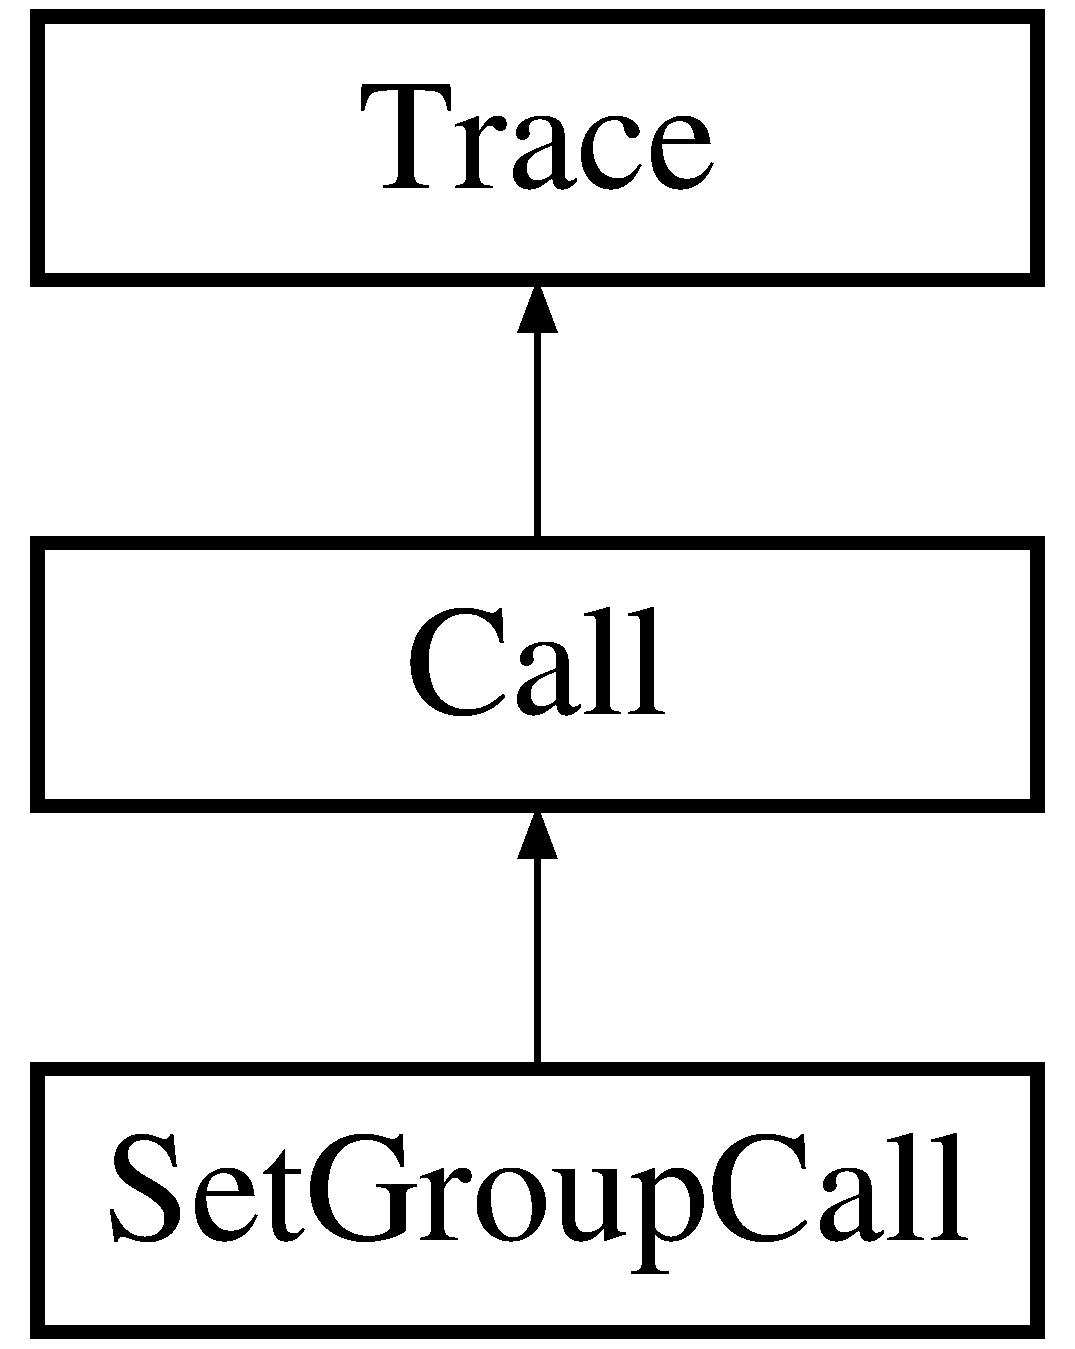
\includegraphics[height=3.000000cm]{class_set_group_call}
\end{center}
\end{figure}
\subsection*{Public Member Functions}
\begin{DoxyCompactItemize}
\item 
\hyperlink{class_set_group_call_a0806e6a027a216a9baaf58cd96d8c09a}{Set\+Group\+Call} (\hyperlink{class_call_ade833a08ce215aaa4121102f3448c898}{Error\+Type} \hyperlink{class_call_a206f6150a8038fda48c17c2c7421aed1}{error}, int unit\+Id, int unit\+Type, int group\+Id)
\item 
\hyperlink{class_set_group_call_ac22755b522982956e681f654be0b5b23}{Set\+Group\+Call} (const \hyperlink{class_set_group_call}{Set\+Group\+Call} $\ast$c)
\item 
virtual \hyperlink{class_trace_a9c58e523529fc8a03fb6acf3eef86150}{Trace\+::sp\+\_\+trace} \hyperlink{class_set_group_call_ac970b30cd2a4769ec134ba451768ee64}{clone} () const 
\begin{DoxyCompactList}\small\item\em Clonage d\textquotesingle{}un appel. \end{DoxyCompactList}\end{DoxyCompactItemize}
\subsection*{Additional Inherited Members}


\subsection{Detailed Description}


Definition at line 409 of file Call\+Def.\+h.



\subsection{Constructor \& Destructor Documentation}
\index{Set\+Group\+Call@{Set\+Group\+Call}!Set\+Group\+Call@{Set\+Group\+Call}}
\index{Set\+Group\+Call@{Set\+Group\+Call}!Set\+Group\+Call@{Set\+Group\+Call}}
\subsubsection[{\texorpdfstring{Set\+Group\+Call(\+Error\+Type error, int unit\+Id, int unit\+Type, int group\+Id)}{SetGroupCall(ErrorType error, int unitId, int unitType, int groupId)}}]{\setlength{\rightskip}{0pt plus 5cm}Set\+Group\+Call\+::\+Set\+Group\+Call (
\begin{DoxyParamCaption}
\item[{{\bf Error\+Type}}]{error, }
\item[{int}]{unit\+Id, }
\item[{int}]{unit\+Type, }
\item[{int}]{group\+Id}
\end{DoxyParamCaption}
)\hspace{0.3cm}{\ttfamily [inline]}}\hypertarget{class_set_group_call_a0806e6a027a216a9baaf58cd96d8c09a}{}\label{class_set_group_call_a0806e6a027a216a9baaf58cd96d8c09a}


Definition at line 413 of file Call\+Def.\+h.

\index{Set\+Group\+Call@{Set\+Group\+Call}!Set\+Group\+Call@{Set\+Group\+Call}}
\index{Set\+Group\+Call@{Set\+Group\+Call}!Set\+Group\+Call@{Set\+Group\+Call}}
\subsubsection[{\texorpdfstring{Set\+Group\+Call(const Set\+Group\+Call $\ast$c)}{SetGroupCall(const SetGroupCall *c)}}]{\setlength{\rightskip}{0pt plus 5cm}Set\+Group\+Call\+::\+Set\+Group\+Call (
\begin{DoxyParamCaption}
\item[{const {\bf Set\+Group\+Call} $\ast$}]{c}
\end{DoxyParamCaption}
)\hspace{0.3cm}{\ttfamily [inline]}}\hypertarget{class_set_group_call_ac22755b522982956e681f654be0b5b23}{}\label{class_set_group_call_ac22755b522982956e681f654be0b5b23}


Definition at line 418 of file Call\+Def.\+h.



\subsection{Member Function Documentation}
\index{Set\+Group\+Call@{Set\+Group\+Call}!clone@{clone}}
\index{clone@{clone}!Set\+Group\+Call@{Set\+Group\+Call}}
\subsubsection[{\texorpdfstring{clone() const }{clone() const }}]{\setlength{\rightskip}{0pt plus 5cm}virtual {\bf Trace\+::sp\+\_\+trace} Set\+Group\+Call\+::clone (
\begin{DoxyParamCaption}
{}
\end{DoxyParamCaption}
) const\hspace{0.3cm}{\ttfamily [inline]}, {\ttfamily [virtual]}}\hypertarget{class_set_group_call_ac970b30cd2a4769ec134ba451768ee64}{}\label{class_set_group_call_ac970b30cd2a4769ec134ba451768ee64}


Clonage d\textquotesingle{}un appel. 

\begin{DoxyReturn}{Returns}
une copie de l\textquotesingle{}objet \hyperlink{class_call}{Call}. 
\end{DoxyReturn}


Implements \hyperlink{class_call_ab3bf0965d35eb1e97ecddaf2d3978e9b}{Call}.



Definition at line 424 of file Call\+Def.\+h.



The documentation for this class was generated from the following file\+:\begin{DoxyCompactItemize}
\item 
C\+:/\+Users/\+Stephane/\+Desktop/mocahteam/\+Prog\+And\+Play/pp/traces/src/\hyperlink{_call_def_8h}{Call\+Def.\+h}\end{DoxyCompactItemize}

\hypertarget{class_start_mission_event}{}\section{Start\+Mission\+Event Class Reference}
\label{class_start_mission_event}\index{Start\+Mission\+Event@{Start\+Mission\+Event}}


{\ttfamily \#include $<$Event\+Def.\+h$>$}

Inheritance diagram for Start\+Mission\+Event\+:\begin{figure}[H]
\begin{center}
\leavevmode
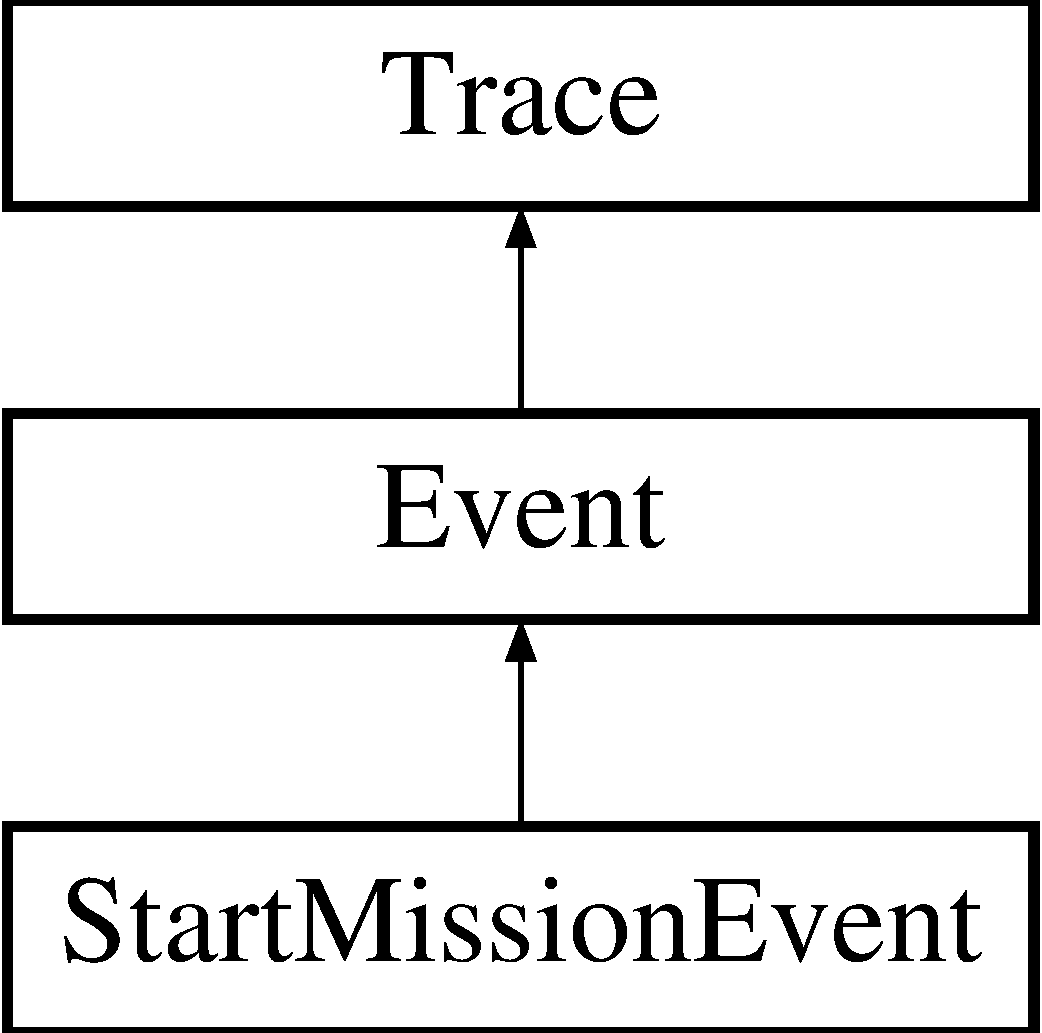
\includegraphics[height=3.000000cm]{class_start_mission_event}
\end{center}
\end{figure}
\subsection*{Public Member Functions}
\begin{DoxyCompactItemize}
\item 
\hyperlink{class_start_mission_event_ad8eb6b28186a393389c733bc1f7d2126}{Start\+Mission\+Event} (std\+::string mission\+\_\+name, int start\+\_\+time)
\item 
\hyperlink{class_start_mission_event_a7eb187e97a54da7f4385724e437db3dc}{Start\+Mission\+Event} (const \hyperlink{class_start_mission_event}{Start\+Mission\+Event} $\ast$sme)
\item 
virtual \hyperlink{class_trace_a9c58e523529fc8a03fb6acf3eef86150}{Trace\+::sp\+\_\+trace} \hyperlink{class_start_mission_event_a4dcda1cb85c391e3594ab1486bc3223d}{clone} () const 
\begin{DoxyCompactList}\small\item\em Clonage d\textquotesingle{}un événement. \end{DoxyCompactList}\item 
virtual std\+::string \hyperlink{class_start_mission_event_a498a3b6e3fa6dfd736486aaa1db421dd}{get\+Params} () const 
\begin{DoxyCompactList}\small\item\em Retourne les différents paramètres relatifs à l\textquotesingle{}événement sous forme de chaîne de caractères. \end{DoxyCompactList}\item 
std\+::string \hyperlink{class_start_mission_event_a605cdb25ede0fbb309816a9175ca250a}{get\+Mission\+Name} () const 
\item 
int \hyperlink{class_start_mission_event_a7fe6b59b37da5c1a25fe5794a4426db6}{get\+Start\+Time} () const 
\end{DoxyCompactItemize}
\subsection*{Additional Inherited Members}


\subsection{Detailed Description}


Definition at line 13 of file Event\+Def.\+h.



\subsection{Constructor \& Destructor Documentation}
\index{Start\+Mission\+Event@{Start\+Mission\+Event}!Start\+Mission\+Event@{Start\+Mission\+Event}}
\index{Start\+Mission\+Event@{Start\+Mission\+Event}!Start\+Mission\+Event@{Start\+Mission\+Event}}
\subsubsection[{\texorpdfstring{Start\+Mission\+Event(std\+::string mission\+\_\+name, int start\+\_\+time)}{StartMissionEvent(std::string mission_name, int start_time)}}]{\setlength{\rightskip}{0pt plus 5cm}Start\+Mission\+Event\+::\+Start\+Mission\+Event (
\begin{DoxyParamCaption}
\item[{std\+::string}]{mission\+\_\+name, }
\item[{int}]{start\+\_\+time}
\end{DoxyParamCaption}
)\hspace{0.3cm}{\ttfamily [inline]}}\hypertarget{class_start_mission_event_ad8eb6b28186a393389c733bc1f7d2126}{}\label{class_start_mission_event_ad8eb6b28186a393389c733bc1f7d2126}


Definition at line 17 of file Event\+Def.\+h.

\index{Start\+Mission\+Event@{Start\+Mission\+Event}!Start\+Mission\+Event@{Start\+Mission\+Event}}
\index{Start\+Mission\+Event@{Start\+Mission\+Event}!Start\+Mission\+Event@{Start\+Mission\+Event}}
\subsubsection[{\texorpdfstring{Start\+Mission\+Event(const Start\+Mission\+Event $\ast$sme)}{StartMissionEvent(const StartMissionEvent *sme)}}]{\setlength{\rightskip}{0pt plus 5cm}Start\+Mission\+Event\+::\+Start\+Mission\+Event (
\begin{DoxyParamCaption}
\item[{const {\bf Start\+Mission\+Event} $\ast$}]{sme}
\end{DoxyParamCaption}
)\hspace{0.3cm}{\ttfamily [inline]}}\hypertarget{class_start_mission_event_a7eb187e97a54da7f4385724e437db3dc}{}\label{class_start_mission_event_a7eb187e97a54da7f4385724e437db3dc}


Definition at line 19 of file Event\+Def.\+h.



\subsection{Member Function Documentation}
\index{Start\+Mission\+Event@{Start\+Mission\+Event}!clone@{clone}}
\index{clone@{clone}!Start\+Mission\+Event@{Start\+Mission\+Event}}
\subsubsection[{\texorpdfstring{clone() const }{clone() const }}]{\setlength{\rightskip}{0pt plus 5cm}virtual {\bf Trace\+::sp\+\_\+trace} Start\+Mission\+Event\+::clone (
\begin{DoxyParamCaption}
{}
\end{DoxyParamCaption}
) const\hspace{0.3cm}{\ttfamily [inline]}, {\ttfamily [virtual]}}\hypertarget{class_start_mission_event_a4dcda1cb85c391e3594ab1486bc3223d}{}\label{class_start_mission_event_a4dcda1cb85c391e3594ab1486bc3223d}


Clonage d\textquotesingle{}un événement. 

\begin{DoxyReturn}{Returns}
une copie de l\textquotesingle{}objet \hyperlink{class_event}{Event}. 
\end{DoxyReturn}


Reimplemented from \hyperlink{class_event_aafa2022d6600717a9cd6511797548265}{Event}.



Definition at line 24 of file Event\+Def.\+h.

\index{Start\+Mission\+Event@{Start\+Mission\+Event}!get\+Mission\+Name@{get\+Mission\+Name}}
\index{get\+Mission\+Name@{get\+Mission\+Name}!Start\+Mission\+Event@{Start\+Mission\+Event}}
\subsubsection[{\texorpdfstring{get\+Mission\+Name() const }{getMissionName() const }}]{\setlength{\rightskip}{0pt plus 5cm}std\+::string Start\+Mission\+Event\+::get\+Mission\+Name (
\begin{DoxyParamCaption}
{}
\end{DoxyParamCaption}
) const\hspace{0.3cm}{\ttfamily [inline]}}\hypertarget{class_start_mission_event_a605cdb25ede0fbb309816a9175ca250a}{}\label{class_start_mission_event_a605cdb25ede0fbb309816a9175ca250a}


Definition at line 32 of file Event\+Def.\+h.

\index{Start\+Mission\+Event@{Start\+Mission\+Event}!get\+Params@{get\+Params}}
\index{get\+Params@{get\+Params}!Start\+Mission\+Event@{Start\+Mission\+Event}}
\subsubsection[{\texorpdfstring{get\+Params() const }{getParams() const }}]{\setlength{\rightskip}{0pt plus 5cm}virtual std\+::string Start\+Mission\+Event\+::get\+Params (
\begin{DoxyParamCaption}
{}
\end{DoxyParamCaption}
) const\hspace{0.3cm}{\ttfamily [inline]}, {\ttfamily [virtual]}}\hypertarget{class_start_mission_event_a498a3b6e3fa6dfd736486aaa1db421dd}{}\label{class_start_mission_event_a498a3b6e3fa6dfd736486aaa1db421dd}


Retourne les différents paramètres relatifs à l\textquotesingle{}événement sous forme de chaîne de caractères. 

Cette fonction doit être redéfinie par les classes héritant de \hyperlink{class_event}{Event}.

\begin{DoxyReturn}{Returns}
la chaîne de caractères formatée contenant les valeurs des différents paramètres de l\textquotesingle{}événement séparées par des espaces. 
\end{DoxyReturn}


Reimplemented from \hyperlink{class_event_aad213c94070547bb727ba369b3460e2a}{Event}.



Definition at line 28 of file Event\+Def.\+h.

\index{Start\+Mission\+Event@{Start\+Mission\+Event}!get\+Start\+Time@{get\+Start\+Time}}
\index{get\+Start\+Time@{get\+Start\+Time}!Start\+Mission\+Event@{Start\+Mission\+Event}}
\subsubsection[{\texorpdfstring{get\+Start\+Time() const }{getStartTime() const }}]{\setlength{\rightskip}{0pt plus 5cm}int Start\+Mission\+Event\+::get\+Start\+Time (
\begin{DoxyParamCaption}
{}
\end{DoxyParamCaption}
) const\hspace{0.3cm}{\ttfamily [inline]}}\hypertarget{class_start_mission_event_a7fe6b59b37da5c1a25fe5794a4426db6}{}\label{class_start_mission_event_a7fe6b59b37da5c1a25fe5794a4426db6}


Definition at line 36 of file Event\+Def.\+h.



The documentation for this class was generated from the following file\+:\begin{DoxyCompactItemize}
\item 
C\+:/\+Users/\+Stephane/\+Desktop/mocahteam/\+Prog\+And\+Play/pp/traces/src/\hyperlink{_event_def_8h}{Event\+Def.\+h}\end{DoxyCompactItemize}

\hypertarget{class_trace}{}\section{Trace Class Reference}
\label{class_trace}\index{Trace@{Trace}}


La classe \hyperlink{class_trace}{Trace} est une classe abstraite servant de classe mère aux classes \hyperlink{class_sequence}{Sequence}, \hyperlink{class_call}{Call} et \hyperlink{class_event}{Event}.  




{\ttfamily \#include $<$Trace.\+h$>$}

Inheritance diagram for Trace\+:\begin{figure}[H]
\begin{center}
\leavevmode
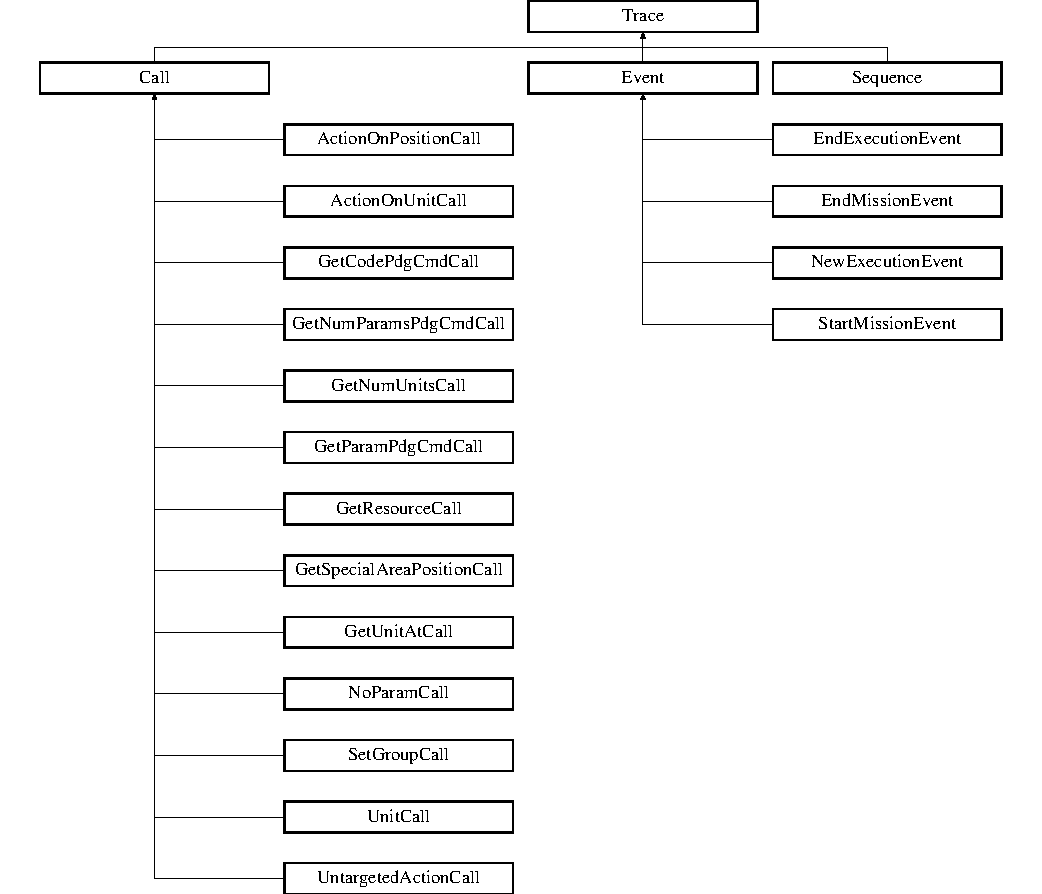
\includegraphics[height=12.000000cm]{class_trace}
\end{center}
\end{figure}
\subsection*{Public Types}
\begin{DoxyCompactItemize}
\item 
enum \hyperlink{class_trace_a39e5f82f2243958348cc74d7cdae527c}{Trace\+Type} \{ \hyperlink{class_trace_a39e5f82f2243958348cc74d7cdae527caebbdad96feb25d8a1b79eafbfc0036c1}{S\+E\+Q\+U\+E\+N\+CE}, 
\hyperlink{class_trace_a39e5f82f2243958348cc74d7cdae527ca15e133d9a16235bbac953dbfa35a5368}{C\+A\+LL}, 
\hyperlink{class_trace_a39e5f82f2243958348cc74d7cdae527caf73b96a847b9877ca903e102074a52df}{E\+V\+E\+NT}
 \}\begin{DoxyCompactList}\small\item\em Enumeration utilisée pour connaître le type de la trace. Une trace peut être de type Trace\+::\+Trace\+Type\+::\+S\+E\+Q\+U\+E\+N\+CE, Trace\+::\+Trace\+Type\+::\+C\+A\+LL ou Trace\+::\+Trace\+Type\+::\+E\+V\+E\+NT. \end{DoxyCompactList}
\item 
typedef boost\+::shared\+\_\+ptr$<$ \hyperlink{class_trace}{Trace} $>$ \hyperlink{class_trace_a9c58e523529fc8a03fb6acf3eef86150}{sp\+\_\+trace}
\end{DoxyCompactItemize}
\subsection*{Public Member Functions}
\begin{DoxyCompactItemize}
\item 
virtual \hyperlink{class_trace_a293f9c9de28b53b0d5edae908b90be03}{$\sim$\+Trace} ()
\begin{DoxyCompactList}\small\item\em Destructeur de \hyperlink{class_trace}{Trace}. \end{DoxyCompactList}\item 
virtual unsigned int \hyperlink{class_trace_a74a29f7e259781424d9f81409ed34701}{length} () const  =0
\begin{DoxyCompactList}\small\item\em Retourne la longueur d\textquotesingle{}une trace. \end{DoxyCompactList}\item 
virtual bool \hyperlink{class_trace_a8201809c2fcc1d02cfa8bf894a79bb5e}{operator==} (\hyperlink{class_trace}{Trace} $\ast$t) const  =0
\begin{DoxyCompactList}\small\item\em Comparaison de la trace avec une trace {\ttfamily t}. \end{DoxyCompactList}\item 
virtual \hyperlink{class_trace_a9c58e523529fc8a03fb6acf3eef86150}{sp\+\_\+trace} \hyperlink{class_trace_a0917758337e37f936713ccaf75b532f2}{clone} () const  =0
\begin{DoxyCompactList}\small\item\em Copie de la trace. \end{DoxyCompactList}\item 
virtual void \hyperlink{class_trace_a4324fa45af235238ddedc2215c3d1cf0}{display} (std\+::ostream \&os=std\+::cout) const  =0
\begin{DoxyCompactList}\small\item\em Affichage de la trace. \end{DoxyCompactList}\item 
virtual void \hyperlink{class_trace_ab152bd0c953d48da2eecda17a1762b18}{reset\+Aligned} ()
\begin{DoxyCompactList}\small\item\em Remise à zéro du pointeur {\ttfamily aligned}. \end{DoxyCompactList}\item 
bool \hyperlink{class_trace_aaa85a39ff507206addd6cfd5a49bbca8}{is\+Sequence} () const 
\begin{DoxyCompactList}\small\item\em Teste si la trace est une séquence. \end{DoxyCompactList}\item 
bool \hyperlink{class_trace_a901bf10475a27420aa2ccd52388bc1fd}{is\+Event} () const 
\begin{DoxyCompactList}\small\item\em Teste si la trace est un event. \end{DoxyCompactList}\item 
bool \hyperlink{class_trace_a65fbddb70261866299cbaabb7c5f019e}{is\+Call} () const 
\begin{DoxyCompactList}\small\item\em Teste si la trace est un call. \end{DoxyCompactList}\item 
bool \hyperlink{class_trace_aabbb4de8e5b5ea0983021688800bd43f}{is\+Delayed} () const 
\begin{DoxyCompactList}\small\item\em Getter pour la variable \hyperlink{class_trace_a9757057cc65f9e45bbeaa848cb06d5a1}{Trace\+::delayed}. \end{DoxyCompactList}\item 
void \hyperlink{class_trace_ae534382e67e6abdf8614a30ebf849d03}{set\+Delayed} ()
\begin{DoxyCompactList}\small\item\em Setter pour la variable \hyperlink{class_trace_a9757057cc65f9e45bbeaa848cb06d5a1}{Trace\+::delayed}. \end{DoxyCompactList}\item 
std\+::string \hyperlink{class_trace_a077c3a0c551e5e898ec0f7cf3911e882}{get\+Info} () const 
\begin{DoxyCompactList}\small\item\em Getter pour la variable {\ttfamily info}. \end{DoxyCompactList}\item 
void \hyperlink{class_trace_a881e1e9879f9db561402f1381fc6fe3e}{set\+Info} (std\+::string \hyperlink{class_trace_a4835dcfa7da5d4c971e8f7d6860acb09}{info})
\begin{DoxyCompactList}\small\item\em Setter pour la variable {\ttfamily info}. \end{DoxyCompactList}\item 
const \hyperlink{class_trace_a9c58e523529fc8a03fb6acf3eef86150}{sp\+\_\+trace} \& \hyperlink{class_trace_a3d82b8d5984686606bf485112be53354}{get\+Parent} () const 
\begin{DoxyCompactList}\small\item\em Getter pour la variable {\ttfamily parent}. \end{DoxyCompactList}\item 
const \hyperlink{class_trace_a9c58e523529fc8a03fb6acf3eef86150}{sp\+\_\+trace} \& \hyperlink{class_trace_aac433090e2cf94657c61e4c73c3bd530}{get\+Aligned} () const 
\begin{DoxyCompactList}\small\item\em Getter pour la variable {\ttfamily aligned}. \end{DoxyCompactList}\item 
void \hyperlink{class_trace_af1973ce75a2b1a1422bfffdfc1b8e4a2}{set\+Parent} (const \hyperlink{class_trace_a9c58e523529fc8a03fb6acf3eef86150}{sp\+\_\+trace} \&spt)
\begin{DoxyCompactList}\small\item\em Setter pour la variable {\ttfamily parent}. \end{DoxyCompactList}\item 
void \hyperlink{class_trace_ae6552786a5c3b35573c106e4910a5881}{set\+Aligned} (const \hyperlink{class_trace_a9c58e523529fc8a03fb6acf3eef86150}{sp\+\_\+trace} \&spt)
\begin{DoxyCompactList}\small\item\em Setter pour la variable {\ttfamily aligned}. \end{DoxyCompactList}\item 
unsigned int \hyperlink{class_trace_af355f36b176399dd35848562ba38ebea}{get\+Level} () const 
\begin{DoxyCompactList}\small\item\em Retoune le niveau de la trace dans la hierarchie globale. \end{DoxyCompactList}\end{DoxyCompactItemize}
\subsection*{Static Public Member Functions}
\begin{DoxyCompactItemize}
\item 
static int \hyperlink{class_trace_ac641a642889e5f527402b45e7c8908a1}{in\+Array} (const char $\ast$ch, const char $\ast$arr\mbox{[}$\,$\mbox{]})
\begin{DoxyCompactList}\small\item\em Recherche d\textquotesingle{}une chaîne de caractères dans un tableau de chaînes de caractères. \end{DoxyCompactList}\item 
static unsigned int \hyperlink{class_trace_a479e20e1158483aa60f656419160da97}{get\+Length} (const std\+::vector$<$ \hyperlink{class_trace_a9c58e523529fc8a03fb6acf3eef86150}{sp\+\_\+trace} $>$ \&traces, int ind\+\_\+start=-\/1, int ind\+\_\+end=-\/1)
\begin{DoxyCompactList}\small\item\em Récupération de la longueur du sous-\/vecteur \mbox{[}ind\+\_\+start,ind\+\_\+end\mbox{[} du vecteur {\ttfamily traces}. \end{DoxyCompactList}\end{DoxyCompactItemize}
\subsection*{Public Attributes}
\begin{DoxyCompactItemize}
\item 
int \hyperlink{class_trace_ae1aa55b6282f5dae12f63b0282ef4b9d}{ind\+Search}
\item 
unsigned int \hyperlink{class_trace_a37d1196b3efa0038af8dcbb7701fcd91}{len\+Search}
\item 
unsigned int \hyperlink{class_trace_a8c8413995806feaeebda9f5360db9dbd}{end\+Search}
\end{DoxyCompactItemize}
\subsection*{Static Public Attributes}
\begin{DoxyCompactItemize}
\item 
static int \hyperlink{class_trace_a21ee84e87f59ed66eb6fa505cc6bf637}{num\+Tab} = 0
\end{DoxyCompactItemize}
\subsection*{Protected Member Functions}
\begin{DoxyCompactItemize}
\item 
\hyperlink{class_trace_a1891c08c9e847b798d2e39f49b2d24b5}{Trace} (\hyperlink{class_trace_a39e5f82f2243958348cc74d7cdae527c}{Trace\+Type} \hyperlink{class_trace_a9f90324e4302d53892143da44cc63054}{type}, std\+::string \hyperlink{class_trace_a4835dcfa7da5d4c971e8f7d6860acb09}{info}=\char`\"{}\char`\"{})
\begin{DoxyCompactList}\small\item\em Constructeur principal de \hyperlink{class_trace}{Trace}. \end{DoxyCompactList}\item 
\hyperlink{class_trace_a586ba22dd795fc2d6ff874d9f7d52929}{Trace} (const \hyperlink{class_trace}{Trace} $\ast$t)
\begin{DoxyCompactList}\small\item\em Constructeur de \hyperlink{class_trace}{Trace} utilisé pour le clonage d\textquotesingle{}une trace. \end{DoxyCompactList}\end{DoxyCompactItemize}
\subsection*{Protected Attributes}
\begin{DoxyCompactItemize}
\item 
\hyperlink{class_trace_a39e5f82f2243958348cc74d7cdae527c}{Trace\+Type} \hyperlink{class_trace_a9f90324e4302d53892143da44cc63054}{type}
\item 
std\+::string \hyperlink{class_trace_a4835dcfa7da5d4c971e8f7d6860acb09}{info}
\item 
bool \hyperlink{class_trace_a9757057cc65f9e45bbeaa848cb06d5a1}{delayed}
\item 
\hyperlink{class_trace_a9c58e523529fc8a03fb6acf3eef86150}{sp\+\_\+trace} \hyperlink{class_trace_a4ace0a20ceb2b0722970be729bd41dc8}{aligned}
\item 
\hyperlink{class_trace_a9c58e523529fc8a03fb6acf3eef86150}{sp\+\_\+trace} \hyperlink{class_trace_a52648b4a6c117072f5797c0e31518f24}{parent}
\end{DoxyCompactItemize}


\subsection{Detailed Description}
La classe \hyperlink{class_trace}{Trace} est une classe abstraite servant de classe mère aux classes \hyperlink{class_sequence}{Sequence}, \hyperlink{class_call}{Call} et \hyperlink{class_event}{Event}. 

Definition at line 22 of file Trace.\+h.



\subsection{Member Typedef Documentation}
\index{Trace@{Trace}!sp\+\_\+trace@{sp\+\_\+trace}}
\index{sp\+\_\+trace@{sp\+\_\+trace}!Trace@{Trace}}
\subsubsection[{\texorpdfstring{sp\+\_\+trace}{sp_trace}}]{\setlength{\rightskip}{0pt plus 5cm}typedef boost\+::shared\+\_\+ptr$<${\bf Trace}$>$ {\bf Trace\+::sp\+\_\+trace}}\hypertarget{class_trace_a9c58e523529fc8a03fb6acf3eef86150}{}\label{class_trace_a9c58e523529fc8a03fb6acf3eef86150}
Définition du type pointeur intelligent vers un objet \hyperlink{class_trace}{Trace}. 

Definition at line 29 of file Trace.\+h.



\subsection{Member Enumeration Documentation}
\index{Trace@{Trace}!Trace\+Type@{Trace\+Type}}
\index{Trace\+Type@{Trace\+Type}!Trace@{Trace}}
\subsubsection[{\texorpdfstring{Trace\+Type}{TraceType}}]{\setlength{\rightskip}{0pt plus 5cm}enum {\bf Trace\+::\+Trace\+Type}}\hypertarget{class_trace_a39e5f82f2243958348cc74d7cdae527c}{}\label{class_trace_a39e5f82f2243958348cc74d7cdae527c}


Enumeration utilisée pour connaître le type de la trace. Une trace peut être de type Trace\+::\+Trace\+Type\+::\+S\+E\+Q\+U\+E\+N\+CE, Trace\+::\+Trace\+Type\+::\+C\+A\+LL ou Trace\+::\+Trace\+Type\+::\+E\+V\+E\+NT. 

\begin{Desc}
\item[Enumerator]\par
\begin{description}
\index{S\+E\+Q\+U\+E\+N\+CE@{S\+E\+Q\+U\+E\+N\+CE}!Trace@{Trace}}\index{Trace@{Trace}!S\+E\+Q\+U\+E\+N\+CE@{S\+E\+Q\+U\+E\+N\+CE}}\item[{\em 
S\+E\+Q\+U\+E\+N\+CE\hypertarget{class_trace_a39e5f82f2243958348cc74d7cdae527caebbdad96feb25d8a1b79eafbfc0036c1}{}\label{class_trace_a39e5f82f2243958348cc74d7cdae527caebbdad96feb25d8a1b79eafbfc0036c1}
}]\index{C\+A\+LL@{C\+A\+LL}!Trace@{Trace}}\index{Trace@{Trace}!C\+A\+LL@{C\+A\+LL}}\item[{\em 
C\+A\+LL\hypertarget{class_trace_a39e5f82f2243958348cc74d7cdae527ca15e133d9a16235bbac953dbfa35a5368}{}\label{class_trace_a39e5f82f2243958348cc74d7cdae527ca15e133d9a16235bbac953dbfa35a5368}
}]\index{E\+V\+E\+NT@{E\+V\+E\+NT}!Trace@{Trace}}\index{Trace@{Trace}!E\+V\+E\+NT@{E\+V\+E\+NT}}\item[{\em 
E\+V\+E\+NT\hypertarget{class_trace_a39e5f82f2243958348cc74d7cdae527caf73b96a847b9877ca903e102074a52df}{}\label{class_trace_a39e5f82f2243958348cc74d7cdae527caf73b96a847b9877ca903e102074a52df}
}]\end{description}
\end{Desc}


Definition at line 34 of file Trace.\+h.



\subsection{Constructor \& Destructor Documentation}
\index{Trace@{Trace}!````~Trace@{$\sim$\+Trace}}
\index{````~Trace@{$\sim$\+Trace}!Trace@{Trace}}
\subsubsection[{\texorpdfstring{$\sim$\+Trace()}{~Trace()}}]{\setlength{\rightskip}{0pt plus 5cm}virtual Trace\+::$\sim$\+Trace (
\begin{DoxyParamCaption}
{}
\end{DoxyParamCaption}
)\hspace{0.3cm}{\ttfamily [inline]}, {\ttfamily [virtual]}}\hypertarget{class_trace_a293f9c9de28b53b0d5edae908b90be03}{}\label{class_trace_a293f9c9de28b53b0d5edae908b90be03}


Destructeur de \hyperlink{class_trace}{Trace}. 



Definition at line 43 of file Trace.\+h.

\index{Trace@{Trace}!Trace@{Trace}}
\index{Trace@{Trace}!Trace@{Trace}}
\subsubsection[{\texorpdfstring{Trace(\+Trace\+Type type, std\+::string info="""")}{Trace(TraceType type, std::string info="")}}]{\setlength{\rightskip}{0pt plus 5cm}Trace\+::\+Trace (
\begin{DoxyParamCaption}
\item[{{\bf Trace\+Type}}]{type, }
\item[{std\+::string}]{info = {\ttfamily \char`\"{}\char`\"{}}}
\end{DoxyParamCaption}
)\hspace{0.3cm}{\ttfamily [protected]}}\hypertarget{class_trace_a1891c08c9e847b798d2e39f49b2d24b5}{}\label{class_trace_a1891c08c9e847b798d2e39f49b2d24b5}


Constructeur principal de \hyperlink{class_trace}{Trace}. 



Definition at line 5 of file Trace.\+cpp.

\index{Trace@{Trace}!Trace@{Trace}}
\index{Trace@{Trace}!Trace@{Trace}}
\subsubsection[{\texorpdfstring{Trace(const Trace $\ast$t)}{Trace(const Trace *t)}}]{\setlength{\rightskip}{0pt plus 5cm}Trace\+::\+Trace (
\begin{DoxyParamCaption}
\item[{const {\bf Trace} $\ast$}]{t}
\end{DoxyParamCaption}
)\hspace{0.3cm}{\ttfamily [protected]}}\hypertarget{class_trace_a586ba22dd795fc2d6ff874d9f7d52929}{}\label{class_trace_a586ba22dd795fc2d6ff874d9f7d52929}


Constructeur de \hyperlink{class_trace}{Trace} utilisé pour le clonage d\textquotesingle{}une trace. 



Definition at line 8 of file Trace.\+cpp.



\subsection{Member Function Documentation}
\index{Trace@{Trace}!clone@{clone}}
\index{clone@{clone}!Trace@{Trace}}
\subsubsection[{\texorpdfstring{clone() const  =0}{clone() const  =0}}]{\setlength{\rightskip}{0pt plus 5cm}virtual {\bf sp\+\_\+trace} Trace\+::clone (
\begin{DoxyParamCaption}
{}
\end{DoxyParamCaption}
) const\hspace{0.3cm}{\ttfamily [pure virtual]}}\hypertarget{class_trace_a0917758337e37f936713ccaf75b532f2}{}\label{class_trace_a0917758337e37f936713ccaf75b532f2}


Copie de la trace. 

\begin{DoxyReturn}{Returns}
un pointeur intelligent vers la nouvelle trace créée suite au clonage. 
\end{DoxyReturn}


Implemented in \hyperlink{class_get_param_pdg_cmd_call_a07b0bec23a831830746b25ca5d44b317}{Get\+Param\+Pdg\+Cmd\+Call}, \hyperlink{class_get_num_params_pdg_cmd_call_ae0633bca77530d2e3ad5bc3a68109c8f}{Get\+Num\+Params\+Pdg\+Cmd\+Call}, \hyperlink{class_get_code_pdg_cmd_call_adad7b71e06c9b81d17b02191401245f5}{Get\+Code\+Pdg\+Cmd\+Call}, \hyperlink{class_untargeted_action_call_a483d86c01a984c4b1e59e339a1f7329e}{Untargeted\+Action\+Call}, \hyperlink{class_action_on_position_call_aa755b6dbfcbd7efd47251556381f6bc3}{Action\+On\+Position\+Call}, \hyperlink{class_action_on_unit_call_ab127ed211f2b34f476cd0f4ef20d6057}{Action\+On\+Unit\+Call}, \hyperlink{class_set_group_call_ac970b30cd2a4769ec134ba451768ee64}{Set\+Group\+Call}, \hyperlink{class_unit_call_a637d309cd3d0bc05849aa7ca20eb5f89}{Unit\+Call}, \hyperlink{class_get_unit_at_call_a228108026f5f8522a6724e1183e1b6bb}{Get\+Unit\+At\+Call}, \hyperlink{class_call_ab3bf0965d35eb1e97ecddaf2d3978e9b}{Call}, \hyperlink{class_get_num_units_call_a279250063949139d58842ae5a6b39b03}{Get\+Num\+Units\+Call}, \hyperlink{class_get_resource_call_adeda1479826fb33c27c76bd8fe711776}{Get\+Resource\+Call}, \hyperlink{class_end_execution_event_aa89f0e0da951077ac408345235b7444b}{End\+Execution\+Event}, \hyperlink{class_sequence_aad8c31973496749c3e57848af2812284}{Sequence}, \hyperlink{class_get_special_area_position_call_ad522313dad00572f50f2a4a84e12dafd}{Get\+Special\+Area\+Position\+Call}, \hyperlink{class_new_execution_event_adc75351c4c45e5161c26138b29e980ed}{New\+Execution\+Event}, \hyperlink{class_event_aafa2022d6600717a9cd6511797548265}{Event}, \hyperlink{class_end_mission_event_a2d851feeb940eb1c73ab05d8cff28d84}{End\+Mission\+Event}, \hyperlink{class_no_param_call_a8488a6947c974711af12b10f89298bf8}{No\+Param\+Call}, and \hyperlink{class_start_mission_event_a4dcda1cb85c391e3594ab1486bc3223d}{Start\+Mission\+Event}.

\index{Trace@{Trace}!display@{display}}
\index{display@{display}!Trace@{Trace}}
\subsubsection[{\texorpdfstring{display(std\+::ostream \&os=std\+::cout) const  =0}{display(std::ostream &os=std::cout) const  =0}}]{\setlength{\rightskip}{0pt plus 5cm}virtual void Trace\+::display (
\begin{DoxyParamCaption}
\item[{std\+::ostream \&}]{os = {\ttfamily std\+:\+:cout}}
\end{DoxyParamCaption}
) const\hspace{0.3cm}{\ttfamily [pure virtual]}}\hypertarget{class_trace_a4324fa45af235238ddedc2215c3d1cf0}{}\label{class_trace_a4324fa45af235238ddedc2215c3d1cf0}


Affichage de la trace. 


\begin{DoxyParams}{Parameters}
{\em os} & \+: le flux de sortie utilisé pour l\textquotesingle{}affichage. \\
\hline
\end{DoxyParams}


Implemented in \hyperlink{class_call_a397f37a434fc1b186ea3460d0c21ff43}{Call}, \hyperlink{class_sequence_a19d7d6f49253cbaae84cc802760c7d38}{Sequence}, and \hyperlink{class_event_ae5465424aa2d50e2e144eae1d84a7ea9}{Event}.

\index{Trace@{Trace}!get\+Aligned@{get\+Aligned}}
\index{get\+Aligned@{get\+Aligned}!Trace@{Trace}}
\subsubsection[{\texorpdfstring{get\+Aligned() const }{getAligned() const }}]{\setlength{\rightskip}{0pt plus 5cm}const {\bf Trace\+::sp\+\_\+trace} \& Trace\+::get\+Aligned (
\begin{DoxyParamCaption}
{}
\end{DoxyParamCaption}
) const}\hypertarget{class_trace_aac433090e2cf94657c61e4c73c3bd530}{}\label{class_trace_aac433090e2cf94657c61e4c73c3bd530}


Getter pour la variable {\ttfamily aligned}. 

\begin{DoxyReturn}{Returns}
une référence constante à la variable {\ttfamily aligned} de la trace. 
\end{DoxyReturn}


Definition at line 49 of file Trace.\+cpp.

\index{Trace@{Trace}!get\+Info@{get\+Info}}
\index{get\+Info@{get\+Info}!Trace@{Trace}}
\subsubsection[{\texorpdfstring{get\+Info() const }{getInfo() const }}]{\setlength{\rightskip}{0pt plus 5cm}std\+::string Trace\+::get\+Info (
\begin{DoxyParamCaption}
{}
\end{DoxyParamCaption}
) const}\hypertarget{class_trace_a077c3a0c551e5e898ec0f7cf3911e882}{}\label{class_trace_a077c3a0c551e5e898ec0f7cf3911e882}


Getter pour la variable {\ttfamily info}. 

\begin{DoxyReturn}{Returns}
la chaîne de caractères {\ttfamily info} de la trace. 
\end{DoxyReturn}


Definition at line 37 of file Trace.\+cpp.

\index{Trace@{Trace}!get\+Length@{get\+Length}}
\index{get\+Length@{get\+Length}!Trace@{Trace}}
\subsubsection[{\texorpdfstring{get\+Length(const std\+::vector$<$ sp\+\_\+trace $>$ \&traces, int ind\+\_\+start=-\/1, int ind\+\_\+end=-\/1)}{getLength(const std::vector< sp_trace > &traces, int ind_start=-1, int ind_end=-1)}}]{\setlength{\rightskip}{0pt plus 5cm}unsigned int Trace\+::get\+Length (
\begin{DoxyParamCaption}
\item[{const std\+::vector$<$ {\bf sp\+\_\+trace} $>$ \&}]{traces, }
\item[{int}]{ind\+\_\+start = {\ttfamily -\/1}, }
\item[{int}]{ind\+\_\+end = {\ttfamily -\/1}}
\end{DoxyParamCaption}
)\hspace{0.3cm}{\ttfamily [static]}}\hypertarget{class_trace_a479e20e1158483aa60f656419160da97}{}\label{class_trace_a479e20e1158483aa60f656419160da97}


Récupération de la longueur du sous-\/vecteur \mbox{[}ind\+\_\+start,ind\+\_\+end\mbox{[} du vecteur {\ttfamily traces}. 


\begin{DoxyParams}{Parameters}
{\em traces} & \+: le vecteur contenant les traces. \\
\hline
{\em ind\+\_\+start} & \+: l\textquotesingle{}indice du début du sous-\/vecteur dans {\ttfamily traces}. Sa valeur par défaut est 0. \\
\hline
{\em ind\+\_\+end} & \+: l\textquotesingle{}indice de fin du sous-\/vecteur dans {\ttfamily traces}. Sa valeur par défaut est traces.\+size().\\
\hline
\end{DoxyParams}
\begin{DoxyReturn}{Returns}
la longueur du sous-\/vecteur calculée. 
\end{DoxyReturn}


Definition at line 85 of file Trace.\+cpp.

\index{Trace@{Trace}!get\+Level@{get\+Level}}
\index{get\+Level@{get\+Level}!Trace@{Trace}}
\subsubsection[{\texorpdfstring{get\+Level() const }{getLevel() const }}]{\setlength{\rightskip}{0pt plus 5cm}unsigned int Trace\+::get\+Level (
\begin{DoxyParamCaption}
{}
\end{DoxyParamCaption}
) const}\hypertarget{class_trace_af355f36b176399dd35848562ba38ebea}{}\label{class_trace_af355f36b176399dd35848562ba38ebea}


Retoune le niveau de la trace dans la hierarchie globale. 

Cette information n\textquotesingle{}est pas stockée et est donc calculée lors de chaque appel à cette fonction (afin d\textquotesingle{}éviter les oublis de mise à jour). Il correspond au nombre de séquences parentes comptées en remontant la hiérarchie à partir de la trace.

\begin{DoxyReturn}{Returns}
le niveau de la trace 
\end{DoxyReturn}


Definition at line 65 of file Trace.\+cpp.

\index{Trace@{Trace}!get\+Parent@{get\+Parent}}
\index{get\+Parent@{get\+Parent}!Trace@{Trace}}
\subsubsection[{\texorpdfstring{get\+Parent() const }{getParent() const }}]{\setlength{\rightskip}{0pt plus 5cm}const {\bf Trace\+::sp\+\_\+trace} \& Trace\+::get\+Parent (
\begin{DoxyParamCaption}
{}
\end{DoxyParamCaption}
) const}\hypertarget{class_trace_a3d82b8d5984686606bf485112be53354}{}\label{class_trace_a3d82b8d5984686606bf485112be53354}


Getter pour la variable {\ttfamily parent}. 

\begin{DoxyReturn}{Returns}
une référence constante à la variable {\ttfamily parent} de la trace. 
\end{DoxyReturn}


Definition at line 45 of file Trace.\+cpp.

\index{Trace@{Trace}!in\+Array@{in\+Array}}
\index{in\+Array@{in\+Array}!Trace@{Trace}}
\subsubsection[{\texorpdfstring{in\+Array(const char $\ast$ch, const char $\ast$arr[])}{inArray(const char *ch, const char *arr[])}}]{\setlength{\rightskip}{0pt plus 5cm}int Trace\+::in\+Array (
\begin{DoxyParamCaption}
\item[{const char $\ast$}]{ch, }
\item[{const char $\ast$}]{arr\mbox{[}$\,$\mbox{]}}
\end{DoxyParamCaption}
)\hspace{0.3cm}{\ttfamily [static]}}\hypertarget{class_trace_ac641a642889e5f527402b45e7c8908a1}{}\label{class_trace_ac641a642889e5f527402b45e7c8908a1}


Recherche d\textquotesingle{}une chaîne de caractères dans un tableau de chaînes de caractères. 


\begin{DoxyParams}{Parameters}
{\em ch} & \+: la chaîne de caractères recherchée dans {\ttfamily arr}. \\
\hline
{\em arr} & \+: le tableau dans lequel est recherchée {\ttfamily ch}. {\ttfamily arr} doit obligatoirement se terminer par N\+U\+LL.\\
\hline
\end{DoxyParams}
\begin{DoxyReturn}{Returns}
-\/1 si {\ttfamily ch} n\textquotesingle{}est pas présent dans {\ttfamily arr}, et l\textquotesingle{}indice de sa position dans {\ttfamily arr} sinon. 
\end{DoxyReturn}


Definition at line 75 of file Trace.\+cpp.

\index{Trace@{Trace}!is\+Call@{is\+Call}}
\index{is\+Call@{is\+Call}!Trace@{Trace}}
\subsubsection[{\texorpdfstring{is\+Call() const }{isCall() const }}]{\setlength{\rightskip}{0pt plus 5cm}bool Trace\+::is\+Call (
\begin{DoxyParamCaption}
{}
\end{DoxyParamCaption}
) const}\hypertarget{class_trace_a65fbddb70261866299cbaabb7c5f019e}{}\label{class_trace_a65fbddb70261866299cbaabb7c5f019e}


Teste si la trace est un call. 

\begin{DoxyReturn}{Returns}
vrai si la trace est un call, faux sinon. 
\end{DoxyReturn}


Definition at line 25 of file Trace.\+cpp.

\index{Trace@{Trace}!is\+Delayed@{is\+Delayed}}
\index{is\+Delayed@{is\+Delayed}!Trace@{Trace}}
\subsubsection[{\texorpdfstring{is\+Delayed() const }{isDelayed() const }}]{\setlength{\rightskip}{0pt plus 5cm}bool Trace\+::is\+Delayed (
\begin{DoxyParamCaption}
{}
\end{DoxyParamCaption}
) const}\hypertarget{class_trace_aabbb4de8e5b5ea0983021688800bd43f}{}\label{class_trace_aabbb4de8e5b5ea0983021688800bd43f}


Getter pour la variable \hyperlink{class_trace_a9757057cc65f9e45bbeaa848cb06d5a1}{Trace\+::delayed}. 

\begin{DoxySeeAlso}{See also}
\hyperlink{class_trace_a9757057cc65f9e45bbeaa848cb06d5a1}{Trace\+::delayed} 
\end{DoxySeeAlso}


Definition at line 29 of file Trace.\+cpp.

\index{Trace@{Trace}!is\+Event@{is\+Event}}
\index{is\+Event@{is\+Event}!Trace@{Trace}}
\subsubsection[{\texorpdfstring{is\+Event() const }{isEvent() const }}]{\setlength{\rightskip}{0pt plus 5cm}bool Trace\+::is\+Event (
\begin{DoxyParamCaption}
{}
\end{DoxyParamCaption}
) const}\hypertarget{class_trace_a901bf10475a27420aa2ccd52388bc1fd}{}\label{class_trace_a901bf10475a27420aa2ccd52388bc1fd}


Teste si la trace est un event. 

\begin{DoxyReturn}{Returns}
vrai si la trace est un event, faux sinon. 
\end{DoxyReturn}


Definition at line 21 of file Trace.\+cpp.

\index{Trace@{Trace}!is\+Sequence@{is\+Sequence}}
\index{is\+Sequence@{is\+Sequence}!Trace@{Trace}}
\subsubsection[{\texorpdfstring{is\+Sequence() const }{isSequence() const }}]{\setlength{\rightskip}{0pt plus 5cm}bool Trace\+::is\+Sequence (
\begin{DoxyParamCaption}
{}
\end{DoxyParamCaption}
) const}\hypertarget{class_trace_aaa85a39ff507206addd6cfd5a49bbca8}{}\label{class_trace_aaa85a39ff507206addd6cfd5a49bbca8}


Teste si la trace est une séquence. 

\begin{DoxyReturn}{Returns}
vrai si la trace est une séquence, faux sinon. 
\end{DoxyReturn}


Definition at line 17 of file Trace.\+cpp.

\index{Trace@{Trace}!length@{length}}
\index{length@{length}!Trace@{Trace}}
\subsubsection[{\texorpdfstring{length() const  =0}{length() const  =0}}]{\setlength{\rightskip}{0pt plus 5cm}virtual unsigned int Trace\+::length (
\begin{DoxyParamCaption}
{}
\end{DoxyParamCaption}
) const\hspace{0.3cm}{\ttfamily [pure virtual]}}\hypertarget{class_trace_a74a29f7e259781424d9f81409ed34701}{}\label{class_trace_a74a29f7e259781424d9f81409ed34701}


Retourne la longueur d\textquotesingle{}une trace. 

Cette fonction est implémentée dans les classes héritant de \hyperlink{class_trace}{Trace}.

\begin{DoxyReturn}{Returns}
la longueur de la trace.
\end{DoxyReturn}
\begin{DoxySeeAlso}{See also}
\hyperlink{class_sequence_a6da226d77ff5150ced893f0b6c83f83a}{Sequence\+::length} 

\hyperlink{class_call_ac94d8a7498716a0131a731963f035905}{Call\+::length} 

\hyperlink{class_event_adc33626b18f2090fba9f58cf0991fdb5}{Event\+::length} 
\end{DoxySeeAlso}


Implemented in \hyperlink{class_call_ac94d8a7498716a0131a731963f035905}{Call}, \hyperlink{class_sequence_a6da226d77ff5150ced893f0b6c83f83a}{Sequence}, and \hyperlink{class_event_adc33626b18f2090fba9f58cf0991fdb5}{Event}.

\index{Trace@{Trace}!operator==@{operator==}}
\index{operator==@{operator==}!Trace@{Trace}}
\subsubsection[{\texorpdfstring{operator==(\+Trace $\ast$t) const  =0}{operator==(Trace *t) const  =0}}]{\setlength{\rightskip}{0pt plus 5cm}virtual bool Trace\+::operator== (
\begin{DoxyParamCaption}
\item[{{\bf Trace} $\ast$}]{t}
\end{DoxyParamCaption}
) const\hspace{0.3cm}{\ttfamily [pure virtual]}}\hypertarget{class_trace_a8201809c2fcc1d02cfa8bf894a79bb5e}{}\label{class_trace_a8201809c2fcc1d02cfa8bf894a79bb5e}


Comparaison de la trace avec une trace {\ttfamily t}. 

Cette fonction est implémentée dans les classes héritant de \hyperlink{class_trace}{Trace}.


\begin{DoxyParams}{Parameters}
{\em t} & \+: la trace utilisée pour la comparaison.\\
\hline
\end{DoxyParams}
\begin{DoxyReturn}{Returns}
vrai si la trace est considérée comme étant égale à {\ttfamily t}, ou faux sinon. 
\end{DoxyReturn}


Implemented in \hyperlink{class_call_a63f6986cf6a599a25705cf05687f6412}{Call}, \hyperlink{class_sequence_a945e1cb29fadc554bc8a3d61f188998c}{Sequence}, and \hyperlink{class_event_a33edb6d4cfa0dc8040a8a7e9e3e326d9}{Event}.

\index{Trace@{Trace}!reset\+Aligned@{reset\+Aligned}}
\index{reset\+Aligned@{reset\+Aligned}!Trace@{Trace}}
\subsubsection[{\texorpdfstring{reset\+Aligned()}{resetAligned()}}]{\setlength{\rightskip}{0pt plus 5cm}void Trace\+::reset\+Aligned (
\begin{DoxyParamCaption}
{}
\end{DoxyParamCaption}
)\hspace{0.3cm}{\ttfamily [virtual]}}\hypertarget{class_trace_ab152bd0c953d48da2eecda17a1762b18}{}\label{class_trace_ab152bd0c953d48da2eecda17a1762b18}


Remise à zéro du pointeur {\ttfamily aligned}. 

Cette fonction permet de supprimer le lien vers une trace avec laquelle cette trace était alignée.

\begin{DoxySeeAlso}{See also}
\hyperlink{class_sequence_aacd81267429077588208d2a040ea51e4}{Sequence\+::reset\+Aligned} 
\end{DoxySeeAlso}


Reimplemented in \hyperlink{class_sequence_aacd81267429077588208d2a040ea51e4}{Sequence}.



Definition at line 61 of file Trace.\+cpp.

\index{Trace@{Trace}!set\+Aligned@{set\+Aligned}}
\index{set\+Aligned@{set\+Aligned}!Trace@{Trace}}
\subsubsection[{\texorpdfstring{set\+Aligned(const sp\+\_\+trace \&spt)}{setAligned(const sp_trace &spt)}}]{\setlength{\rightskip}{0pt plus 5cm}void Trace\+::set\+Aligned (
\begin{DoxyParamCaption}
\item[{const {\bf sp\+\_\+trace} \&}]{spt}
\end{DoxyParamCaption}
)}\hypertarget{class_trace_ae6552786a5c3b35573c106e4910a5881}{}\label{class_trace_ae6552786a5c3b35573c106e4910a5881}


Setter pour la variable {\ttfamily aligned}. 


\begin{DoxyParams}{Parameters}
{\em spt} & la nouvelle valeur pour la variable {\ttfamily aligned} de la trace. \\
\hline
\end{DoxyParams}


Definition at line 57 of file Trace.\+cpp.

\index{Trace@{Trace}!set\+Delayed@{set\+Delayed}}
\index{set\+Delayed@{set\+Delayed}!Trace@{Trace}}
\subsubsection[{\texorpdfstring{set\+Delayed()}{setDelayed()}}]{\setlength{\rightskip}{0pt plus 5cm}void Trace\+::set\+Delayed (
\begin{DoxyParamCaption}
{}
\end{DoxyParamCaption}
)}\hypertarget{class_trace_ae534382e67e6abdf8614a30ebf849d03}{}\label{class_trace_ae534382e67e6abdf8614a30ebf849d03}


Setter pour la variable \hyperlink{class_trace_a9757057cc65f9e45bbeaa848cb06d5a1}{Trace\+::delayed}. 

La variable \hyperlink{class_trace_a9757057cc65f9e45bbeaa848cb06d5a1}{Trace\+::delayed} est mise à vraie.

\begin{DoxySeeAlso}{See also}
\hyperlink{class_trace_a9757057cc65f9e45bbeaa848cb06d5a1}{Trace\+::delayed} 
\end{DoxySeeAlso}


Definition at line 33 of file Trace.\+cpp.

\index{Trace@{Trace}!set\+Info@{set\+Info}}
\index{set\+Info@{set\+Info}!Trace@{Trace}}
\subsubsection[{\texorpdfstring{set\+Info(std\+::string info)}{setInfo(std::string info)}}]{\setlength{\rightskip}{0pt plus 5cm}void Trace\+::set\+Info (
\begin{DoxyParamCaption}
\item[{std\+::string}]{info}
\end{DoxyParamCaption}
)}\hypertarget{class_trace_a881e1e9879f9db561402f1381fc6fe3e}{}\label{class_trace_a881e1e9879f9db561402f1381fc6fe3e}


Setter pour la variable {\ttfamily info}. 


\begin{DoxyParams}{Parameters}
{\em info} & la nouvelle valeur du champ {\ttfamily info} pour la trace. \\
\hline
\end{DoxyParams}


Definition at line 41 of file Trace.\+cpp.

\index{Trace@{Trace}!set\+Parent@{set\+Parent}}
\index{set\+Parent@{set\+Parent}!Trace@{Trace}}
\subsubsection[{\texorpdfstring{set\+Parent(const sp\+\_\+trace \&spt)}{setParent(const sp_trace &spt)}}]{\setlength{\rightskip}{0pt plus 5cm}void Trace\+::set\+Parent (
\begin{DoxyParamCaption}
\item[{const {\bf sp\+\_\+trace} \&}]{spt}
\end{DoxyParamCaption}
)}\hypertarget{class_trace_af1973ce75a2b1a1422bfffdfc1b8e4a2}{}\label{class_trace_af1973ce75a2b1a1422bfffdfc1b8e4a2}


Setter pour la variable {\ttfamily parent}. 

Cette méthode est utilisée dans \hyperlink{class_sequence_a74e000d0651eb8d4c7bfd20032440c07}{Sequence\+::add\+Trace} pour définir comme parent de la trace la séquence dans laquelle on l\textquotesingle{}ajoute.


\begin{DoxyParams}{Parameters}
{\em spt} & le nouveau {\ttfamily parent} de la trace. \\
\hline
\end{DoxyParams}


Definition at line 53 of file Trace.\+cpp.



\subsection{Member Data Documentation}
\index{Trace@{Trace}!aligned@{aligned}}
\index{aligned@{aligned}!Trace@{Trace}}
\subsubsection[{\texorpdfstring{aligned}{aligned}}]{\setlength{\rightskip}{0pt plus 5cm}{\bf sp\+\_\+trace} Trace\+::aligned\hspace{0.3cm}{\ttfamily [protected]}}\hypertarget{class_trace_a4ace0a20ceb2b0722970be729bd41dc8}{}\label{class_trace_a4ace0a20ceb2b0722970be729bd41dc8}
Contient un pointeur vers la trace alignée avec cette trace durant la phase d\textquotesingle{}alignement.

\begin{DoxySeeAlso}{See also}
Traces\+Analyser\+::find\+Best\+Alignment 
\end{DoxySeeAlso}


Definition at line 262 of file Trace.\+h.

\index{Trace@{Trace}!delayed@{delayed}}
\index{delayed@{delayed}!Trace@{Trace}}
\subsubsection[{\texorpdfstring{delayed}{delayed}}]{\setlength{\rightskip}{0pt plus 5cm}bool Trace\+::delayed\hspace{0.3cm}{\ttfamily [protected]}}\hypertarget{class_trace_a9757057cc65f9e45bbeaa848cb06d5a1}{}\label{class_trace_a9757057cc65f9e45bbeaa848cb06d5a1}
Un booléen mis à vrai lorsque la trace a été générée par le moteur alors que la mission était déjà terminée. 

Definition at line 255 of file Trace.\+h.

\index{Trace@{Trace}!end\+Search@{end\+Search}}
\index{end\+Search@{end\+Search}!Trace@{Trace}}
\subsubsection[{\texorpdfstring{end\+Search}{endSearch}}]{\setlength{\rightskip}{0pt plus 5cm}unsigned int Trace\+::end\+Search}\hypertarget{class_trace_a8c8413995806feaeebda9f5360db9dbd}{}\label{class_trace_a8c8413995806feaeebda9f5360db9dbd}
Compteur utilisé pour stopper et éviter toute future recherche de répétitions d\textquotesingle{}un groupe de traces à partir de la trace possédant cette variable lorsque sa valeur a atteint un certain seuil M\+A\+X\+\_\+\+E\+N\+D\+\_\+\+S\+E\+A\+R\+CH défini dans le fichier \hyperlink{_traces_parser_8h}{Traces\+Parser.\+h}.

\begin{DoxySeeAlso}{See also}
Traces\+Parser\+::detect\+Sequences 
\end{DoxySeeAlso}


Definition at line 137 of file Trace.\+h.

\index{Trace@{Trace}!ind\+Search@{ind\+Search}}
\index{ind\+Search@{ind\+Search}!Trace@{Trace}}
\subsubsection[{\texorpdfstring{ind\+Search}{indSearch}}]{\setlength{\rightskip}{0pt plus 5cm}int Trace\+::ind\+Search}\hypertarget{class_trace_ae1aa55b6282f5dae12f63b0282ef4b9d}{}\label{class_trace_ae1aa55b6282f5dae12f63b0282ef4b9d}
Indice de la trace dans Traces\+Parser\+::traces sur laquelle est placé le curseur lors de la recherche de répétitions d\textquotesingle{}un groupe de traces à partir de la trace possédant cette variable.

\begin{DoxySeeAlso}{See also}
Traces\+Parser\+::detect\+Sequences 
\end{DoxySeeAlso}


Definition at line 123 of file Trace.\+h.

\index{Trace@{Trace}!info@{info}}
\index{info@{info}!Trace@{Trace}}
\subsubsection[{\texorpdfstring{info}{info}}]{\setlength{\rightskip}{0pt plus 5cm}std\+::string Trace\+::info\hspace{0.3cm}{\ttfamily [protected]}}\hypertarget{class_trace_a4835dcfa7da5d4c971e8f7d6860acb09}{}\label{class_trace_a4835dcfa7da5d4c971e8f7d6860acb09}
Un label ajouté par l\textquotesingle{}expert dans le fichier X\+ML utilisé pour l\textquotesingle{}import. 

Definition at line 250 of file Trace.\+h.

\index{Trace@{Trace}!len\+Search@{len\+Search}}
\index{len\+Search@{len\+Search}!Trace@{Trace}}
\subsubsection[{\texorpdfstring{len\+Search}{lenSearch}}]{\setlength{\rightskip}{0pt plus 5cm}unsigned int Trace\+::len\+Search}\hypertarget{class_trace_a37d1196b3efa0038af8dcbb7701fcd91}{}\label{class_trace_a37d1196b3efa0038af8dcbb7701fcd91}
La somme des longueurs des traces contenues dans le vecteur Traces\+Parser\+::traces et comprise entre la trace qui se trouve à la position \hyperlink{class_trace_ae1aa55b6282f5dae12f63b0282ef4b9d}{Trace\+::ind\+Search} (incluse) et celle possédant cette variable (excluse).

\begin{DoxySeeAlso}{See also}
Traces\+Parser\+::detect\+Sequences 
\end{DoxySeeAlso}


Definition at line 130 of file Trace.\+h.

\index{Trace@{Trace}!num\+Tab@{num\+Tab}}
\index{num\+Tab@{num\+Tab}!Trace@{Trace}}
\subsubsection[{\texorpdfstring{num\+Tab}{numTab}}]{\setlength{\rightskip}{0pt plus 5cm}int Trace\+::num\+Tab = 0\hspace{0.3cm}{\ttfamily [static]}}\hypertarget{class_trace_a21ee84e87f59ed66eb6fa505cc6bf637}{}\label{class_trace_a21ee84e87f59ed66eb6fa505cc6bf637}
Variable utilisée pour obtenir une indentation valide des traces lors de leur affichage. 

Definition at line 116 of file Trace.\+h.

\index{Trace@{Trace}!parent@{parent}}
\index{parent@{parent}!Trace@{Trace}}
\subsubsection[{\texorpdfstring{parent}{parent}}]{\setlength{\rightskip}{0pt plus 5cm}{\bf sp\+\_\+trace} Trace\+::parent\hspace{0.3cm}{\ttfamily [protected]}}\hypertarget{class_trace_a52648b4a6c117072f5797c0e31518f24}{}\label{class_trace_a52648b4a6c117072f5797c0e31518f24}
Contient un pointeur vers la séquence contenant cette trace. Si le pointeur est à 0, la trace n\textquotesingle{}a pas de parent. Si le pointeur pointe vers un objet, cet objet est forcément une séquence. 

Definition at line 268 of file Trace.\+h.

\index{Trace@{Trace}!type@{type}}
\index{type@{type}!Trace@{Trace}}
\subsubsection[{\texorpdfstring{type}{type}}]{\setlength{\rightskip}{0pt plus 5cm}{\bf Trace\+Type} Trace\+::type\hspace{0.3cm}{\ttfamily [protected]}}\hypertarget{class_trace_a9f90324e4302d53892143da44cc63054}{}\label{class_trace_a9f90324e4302d53892143da44cc63054}
Le type de la trace. Une trace peut-\/être de type C\+A\+LL, E\+V\+E\+NT ou S\+E\+Q\+U\+E\+N\+CE. 

Definition at line 245 of file Trace.\+h.



The documentation for this class was generated from the following files\+:\begin{DoxyCompactItemize}
\item 
C\+:/\+Users/\+Stephane/\+Desktop/mocahteam/\+Prog\+And\+Play/pp/traces/src/\hyperlink{_trace_8h}{Trace.\+h}\item 
C\+:/\+Users/\+Stephane/\+Desktop/mocahteam/\+Prog\+And\+Play/pp/traces/src/\hyperlink{_trace_8cpp}{Trace.\+cpp}\end{DoxyCompactItemize}

\hypertarget{class_traces_analyser}{}\section{Traces\+Analyser Class Reference}
\label{class_traces_analyser}\index{Traces\+Analyser@{Traces\+Analyser}}


La classe \hyperlink{class_traces_analyser}{Traces\+Analyser} définit l\textquotesingle{}ensemble des traitements relatifs à l\textquotesingle{}analyse des traces.  




{\ttfamily \#include $<$Traces\+Analyser.\+h$>$}

\subsection*{Classes}
\begin{DoxyCompactItemize}
\item 
struct \hyperlink{struct_traces_analyser_1_1_feedback}{Feedback}
\item 
struct \hyperlink{struct_traces_analyser_1_1_game_infos}{Game\+Infos}
\end{DoxyCompactItemize}
\subsection*{Public Types}
\begin{DoxyCompactItemize}
\item 
enum \hyperlink{class_traces_analyser_a57be29ce5ac10ca51e56d8385b4a1820}{Feedback\+Type} \{ \\*
\hyperlink{class_traces_analyser_a57be29ce5ac10ca51e56d8385b4a1820a30a02bf0d89826bac04b59a3723f6225}{N\+O\+NE} = -\/1, 
\hyperlink{class_traces_analyser_a57be29ce5ac10ca51e56d8385b4a1820a08d214704090ad0ead7d60fc2775f2c3}{U\+S\+E\+F\+U\+L\+\_\+\+C\+A\+LL}, 
\hyperlink{class_traces_analyser_a57be29ce5ac10ca51e56d8385b4a1820a08b0a1ea5237d7bab9b09490e7e30b42}{U\+S\+E\+L\+E\+S\+S\+\_\+\+C\+A\+LL}, 
\hyperlink{class_traces_analyser_a57be29ce5ac10ca51e56d8385b4a1820a1b8c8e95fab1f4dde6d38848785a7e08}{S\+E\+Q\+\_\+\+E\+X\+T\+RA}, 
\\*
\hyperlink{class_traces_analyser_a57be29ce5ac10ca51e56d8385b4a1820acd30979f43c0fd19d60770022386222d}{S\+E\+Q\+\_\+\+L\+A\+CK}, 
\hyperlink{class_traces_analyser_a57be29ce5ac10ca51e56d8385b4a1820a6ed25d15ae1133d3fa4a095e38f274ad}{I\+N\+D\+\_\+\+S\+E\+Q\+\_\+\+N\+UM}, 
\hyperlink{class_traces_analyser_a57be29ce5ac10ca51e56d8385b4a1820aea74b14f216c72b2b6ef13ebe16b48f4}{D\+I\+S\+T\+\_\+\+S\+E\+Q\+\_\+\+N\+UM}, 
\hyperlink{class_traces_analyser_a57be29ce5ac10ca51e56d8385b4a1820a14b0fc808a62906ab67aa4b182fe823c}{C\+A\+L\+L\+\_\+\+E\+X\+T\+RA}, 
\\*
\hyperlink{class_traces_analyser_a57be29ce5ac10ca51e56d8385b4a1820a6bdc7824ca798742b8ff903b2c3de12f}{C\+A\+L\+L\+\_\+\+L\+A\+CK}, 
\hyperlink{class_traces_analyser_a57be29ce5ac10ca51e56d8385b4a1820a7ed621eaa247a6d92a9b78e3f3359bf5}{C\+A\+L\+L\+\_\+\+P\+A\+R\+A\+MS}
 \}
\item 
typedef std\+::vector$<$ std\+::pair$<$ int, int $>$ $>$ \hyperlink{class_traces_analyser_a07dca9f55e9ec0dad64e9bf14d329003}{path}
\end{DoxyCompactItemize}
\subsection*{Public Member Functions}
\begin{DoxyCompactItemize}
\item 
\hyperlink{class_traces_analyser_a3e6e883ed6bc74f787684f1a3c0c7c01}{Traces\+Analyser} (std\+::string lang=\char`\"{}fr\char`\"{})
\begin{DoxyCompactList}\small\item\em Constructeur principal de la classe \hyperlink{class_traces_analyser}{Traces\+Analyser}. \end{DoxyCompactList}\item 
std\+::string \hyperlink{class_traces_analyser_aff9ec49bcec7d983dc41c97d452b3e94}{construct\+Feedback} (const std\+::string \&learner\+\_\+xml, const std\+::vector$<$ std\+::string $>$ \&experts\+\_\+xml, int ind\+\_\+mission=-\/1, int ind\+\_\+execution=-\/1, std\+::ostream \&os=std\+::cout)
\begin{DoxyCompactList}\small\item\em Fonction principale d\textquotesingle{}analyse des traces. \end{DoxyCompactList}\item 
void \hyperlink{class_traces_analyser_aead7e56360dc6778a99ccdb63ac63f1e}{load\+Xml\+Infos} (const std\+::string \&feedbacks\+\_\+xml, const std\+::string \&mission\+\_\+feedbacks\+\_\+xml)
\begin{DoxyCompactList}\small\item\em Chargement des feedbacks et des messages contenus dans les fichiers X\+ML \textquotesingle{}feedbacks.\+xml\textquotesingle{}. \end{DoxyCompactList}\item 
void \hyperlink{class_traces_analyser_a76a830a7ca35812b578d2255fb1a6fe9}{set\+Endless\+Loop} (bool endless\+\_\+loop)
\begin{DoxyCompactList}\small\item\em Setter pour la variable {\ttfamily endless\+\_\+loop}. \end{DoxyCompactList}\item 
void \hyperlink{class_traces_analyser_a9726338ac15091c533c9562942d062e1}{set\+Lang} (std\+::string lang)
\begin{DoxyCompactList}\small\item\em Setter pour la variable {\ttfamily lang}. \end{DoxyCompactList}\end{DoxyCompactItemize}
\subsection*{Static Public Member Functions}
\begin{DoxyCompactItemize}
\item 
static int \hyperlink{class_traces_analyser_aefd7da818aa52292e7e9d4df9a7b2be0}{get\+Random\+Int\+In\+Range} (int max)
\begin{DoxyCompactList}\small\item\em Génération aléatoire d\textquotesingle{}un entier compris dans l\textquotesingle{}intervalle \mbox{[}0,max\mbox{[}. \end{DoxyCompactList}\item 
static bool \hyperlink{class_traces_analyser_aa2f744bc8abc8acfbb1407163c36c0b8}{feedback\+Type\+In} (\hyperlink{class_traces_analyser_a57be29ce5ac10ca51e56d8385b4a1820}{Feedback\+Type} type, int n,...)
\begin{DoxyCompactList}\small\item\em Test d\textquotesingle{}appartenance de {\ttfamily type} à un ensemble de valeurs. \end{DoxyCompactList}\item 
static bool \hyperlink{class_traces_analyser_a0ffe68d882d091ec904aa15ab795ec8a}{is\+Expert\+Related\+Feedback} (\hyperlink{class_traces_analyser_a57be29ce5ac10ca51e56d8385b4a1820}{Feedback\+Type} type)
\begin{DoxyCompactList}\small\item\em Test si la valeur de {\ttfamily type} est égale à l\textquotesingle{}une des valeurs suivantes \+: U\+S\+E\+F\+U\+L\+\_\+\+C\+A\+LL, S\+E\+Q\+\_\+\+L\+A\+CK, D\+I\+S\+T\+\_\+\+S\+E\+Q\+\_\+\+N\+UM, I\+N\+D\+\_\+\+S\+E\+Q\+\_\+\+N\+UM, C\+A\+L\+L\+\_\+\+L\+A\+CK, C\+A\+L\+L\+\_\+\+P\+A\+R\+A\+MS. \end{DoxyCompactList}\item 
static bool \hyperlink{class_traces_analyser_ab4bf5099acb58320a75f6540ba3730e2}{is\+Learner\+Related\+Feedback} (\hyperlink{class_traces_analyser_a57be29ce5ac10ca51e56d8385b4a1820}{Feedback\+Type} type)
\begin{DoxyCompactList}\small\item\em Test si la valeur de {\ttfamily type} est égale à l\textquotesingle{}une des valeurs suivantes \+: U\+S\+E\+L\+E\+S\+S\+\_\+\+C\+A\+LL, S\+E\+Q\+\_\+\+E\+X\+T\+RA, D\+I\+S\+T\+\_\+\+S\+E\+Q\+\_\+\+N\+UM, I\+N\+D\+\_\+\+S\+E\+Q\+\_\+\+N\+UM, C\+A\+L\+L\+\_\+\+E\+X\+T\+RA, C\+A\+L\+L\+\_\+\+P\+A\+R\+A\+MS. \end{DoxyCompactList}\end{DoxyCompactItemize}
\subsection*{Static Public Attributes}
\begin{DoxyCompactItemize}
\item 
static const char $\ast$ \hyperlink{class_traces_analyser_af1de6c1349fdad93945a0d8079451d22}{feedback\+Types\+Arr} \mbox{[}$\,$\mbox{]} = \{\char`\"{}useful\+\_\+call\char`\"{}, \char`\"{}useless\+\_\+call\char`\"{}, \char`\"{}seq\+\_\+extra\char`\"{}, \char`\"{}seq\+\_\+lack\char`\"{}, \char`\"{}ind\+\_\+seq\+\_\+num\char`\"{}, \char`\"{}dist\+\_\+seq\+\_\+num\char`\"{}, \char`\"{}call\+\_\+extra\char`\"{}, \char`\"{}call\+\_\+lack\char`\"{}, \char`\"{}call\+\_\+params\char`\"{}, N\+U\+LL\}
\item 
static std\+::map$<$ int, std\+::string $>$ \hyperlink{class_traces_analyser_a5e748c4f52e6cbad197b08c7e0273cd8}{units\+\_\+id\+\_\+map}
\item 
static std\+::map$<$ int, std\+::string $>$ \hyperlink{class_traces_analyser_ac37a3052687b9fc98c38e8ca870157be}{orders\+\_\+map}
\item 
static std\+::map$<$ int, std\+::string $>$ \hyperlink{class_traces_analyser_af64ea0a819c3a124563fe7d0ff6e455f}{resources\+\_\+map}
\item 
static std\+::map$<$ std\+::string, std\+::string $>$ \hyperlink{class_traces_analyser_a2addfbe4fff91dcaa53b83163144bf45}{messages\+\_\+map}
\end{DoxyCompactItemize}


\subsection{Detailed Description}
La classe \hyperlink{class_traces_analyser}{Traces\+Analyser} définit l\textquotesingle{}ensemble des traitements relatifs à l\textquotesingle{}analyse des traces. 

Definition at line 98 of file Traces\+Analyser.\+h.



\subsection{Member Typedef Documentation}
\index{Traces\+Analyser@{Traces\+Analyser}!path@{path}}
\index{path@{path}!Traces\+Analyser@{Traces\+Analyser}}
\subsubsection[{\texorpdfstring{path}{path}}]{\setlength{\rightskip}{0pt plus 5cm}typedef std\+::vector$<$ std\+::pair$<$int,int$>$ $>$ {\bf Traces\+Analyser\+::path}}\hypertarget{class_traces_analyser_a07dca9f55e9ec0dad64e9bf14d329003}{}\label{class_traces_analyser_a07dca9f55e9ec0dad64e9bf14d329003}


Definition at line 102 of file Traces\+Analyser.\+h.



\subsection{Member Enumeration Documentation}
\index{Traces\+Analyser@{Traces\+Analyser}!Feedback\+Type@{Feedback\+Type}}
\index{Feedback\+Type@{Feedback\+Type}!Traces\+Analyser@{Traces\+Analyser}}
\subsubsection[{\texorpdfstring{Feedback\+Type}{FeedbackType}}]{\setlength{\rightskip}{0pt plus 5cm}enum {\bf Traces\+Analyser\+::\+Feedback\+Type}}\hypertarget{class_traces_analyser_a57be29ce5ac10ca51e56d8385b4a1820}{}\label{class_traces_analyser_a57be29ce5ac10ca51e56d8385b4a1820}
Enumération utilisée pour connaître le type de feedback. \begin{Desc}
\item[Enumerator]\par
\begin{description}
\index{N\+O\+NE@{N\+O\+NE}!Traces\+Analyser@{Traces\+Analyser}}\index{Traces\+Analyser@{Traces\+Analyser}!N\+O\+NE@{N\+O\+NE}}\item[{\em 
N\+O\+NE\hypertarget{class_traces_analyser_a57be29ce5ac10ca51e56d8385b4a1820a30a02bf0d89826bac04b59a3723f6225}{}\label{class_traces_analyser_a57be29ce5ac10ca51e56d8385b4a1820a30a02bf0d89826bac04b59a3723f6225}
}]\index{U\+S\+E\+F\+U\+L\+\_\+\+C\+A\+LL@{U\+S\+E\+F\+U\+L\+\_\+\+C\+A\+LL}!Traces\+Analyser@{Traces\+Analyser}}\index{Traces\+Analyser@{Traces\+Analyser}!U\+S\+E\+F\+U\+L\+\_\+\+C\+A\+LL@{U\+S\+E\+F\+U\+L\+\_\+\+C\+A\+LL}}\item[{\em 
U\+S\+E\+F\+U\+L\+\_\+\+C\+A\+LL\hypertarget{class_traces_analyser_a57be29ce5ac10ca51e56d8385b4a1820a08d214704090ad0ead7d60fc2775f2c3}{}\label{class_traces_analyser_a57be29ce5ac10ca51e56d8385b4a1820a08d214704090ad0ead7d60fc2775f2c3}
}]La plupart des experts ont utilisé cet appel mais pas le joueur. Paramétrable avec Traces\+Analyser\+::\+U\+S\+E\+F\+U\+L\+\_\+\+F\+R\+EQ. \index{U\+S\+E\+L\+E\+S\+S\+\_\+\+C\+A\+LL@{U\+S\+E\+L\+E\+S\+S\+\_\+\+C\+A\+LL}!Traces\+Analyser@{Traces\+Analyser}}\index{Traces\+Analyser@{Traces\+Analyser}!U\+S\+E\+L\+E\+S\+S\+\_\+\+C\+A\+LL@{U\+S\+E\+L\+E\+S\+S\+\_\+\+C\+A\+LL}}\item[{\em 
U\+S\+E\+L\+E\+S\+S\+\_\+\+C\+A\+LL\hypertarget{class_traces_analyser_a57be29ce5ac10ca51e56d8385b4a1820a08b0a1ea5237d7bab9b09490e7e30b42}{}\label{class_traces_analyser_a57be29ce5ac10ca51e56d8385b4a1820a08b0a1ea5237d7bab9b09490e7e30b42}
}]le joueur a utilisé cet appel mais très peu d\textquotesingle{}experts l\textquotesingle{}ont utilisé. Paramétrable avec Traces\+Analyser\+::\+U\+S\+E\+L\+E\+S\+S\+\_\+\+F\+R\+EQ. \index{S\+E\+Q\+\_\+\+E\+X\+T\+RA@{S\+E\+Q\+\_\+\+E\+X\+T\+RA}!Traces\+Analyser@{Traces\+Analyser}}\index{Traces\+Analyser@{Traces\+Analyser}!S\+E\+Q\+\_\+\+E\+X\+T\+RA@{S\+E\+Q\+\_\+\+E\+X\+T\+RA}}\item[{\em 
S\+E\+Q\+\_\+\+E\+X\+T\+RA\hypertarget{class_traces_analyser_a57be29ce5ac10ca51e56d8385b4a1820a1b8c8e95fab1f4dde6d38848785a7e08}{}\label{class_traces_analyser_a57be29ce5ac10ca51e56d8385b4a1820a1b8c8e95fab1f4dde6d38848785a7e08}
}]Une séquence non présente dans les traces de l\textquotesingle{}expert est présente dans les traces du joueur. \index{S\+E\+Q\+\_\+\+L\+A\+CK@{S\+E\+Q\+\_\+\+L\+A\+CK}!Traces\+Analyser@{Traces\+Analyser}}\index{Traces\+Analyser@{Traces\+Analyser}!S\+E\+Q\+\_\+\+L\+A\+CK@{S\+E\+Q\+\_\+\+L\+A\+CK}}\item[{\em 
S\+E\+Q\+\_\+\+L\+A\+CK\hypertarget{class_traces_analyser_a57be29ce5ac10ca51e56d8385b4a1820acd30979f43c0fd19d60770022386222d}{}\label{class_traces_analyser_a57be29ce5ac10ca51e56d8385b4a1820acd30979f43c0fd19d60770022386222d}
}]Une séquence non présente dans les traces du joueur est présente dans les traces de l\textquotesingle{}expert. \index{I\+N\+D\+\_\+\+S\+E\+Q\+\_\+\+N\+UM@{I\+N\+D\+\_\+\+S\+E\+Q\+\_\+\+N\+UM}!Traces\+Analyser@{Traces\+Analyser}}\index{Traces\+Analyser@{Traces\+Analyser}!I\+N\+D\+\_\+\+S\+E\+Q\+\_\+\+N\+UM@{I\+N\+D\+\_\+\+S\+E\+Q\+\_\+\+N\+UM}}\item[{\em 
I\+N\+D\+\_\+\+S\+E\+Q\+\_\+\+N\+UM\hypertarget{class_traces_analyser_a57be29ce5ac10ca51e56d8385b4a1820a6ed25d15ae1133d3fa4a095e38f274ad}{}\label{class_traces_analyser_a57be29ce5ac10ca51e56d8385b4a1820a6ed25d15ae1133d3fa4a095e38f274ad}
}]L\textquotesingle{}attribut de la séquence experte \hyperlink{class_sequence_ae495f3d3267ac936660920ab13b2316e}{Sequence\+::num\+\_\+fixed} est à true. La séquence experte est alignée avec une séquence présente dans les traces du joueur. Les deux séquences se trouvent sous la racine. Les indices des deux séquences diffèrent. \index{D\+I\+S\+T\+\_\+\+S\+E\+Q\+\_\+\+N\+UM@{D\+I\+S\+T\+\_\+\+S\+E\+Q\+\_\+\+N\+UM}!Traces\+Analyser@{Traces\+Analyser}}\index{Traces\+Analyser@{Traces\+Analyser}!D\+I\+S\+T\+\_\+\+S\+E\+Q\+\_\+\+N\+UM@{D\+I\+S\+T\+\_\+\+S\+E\+Q\+\_\+\+N\+UM}}\item[{\em 
D\+I\+S\+T\+\_\+\+S\+E\+Q\+\_\+\+N\+UM\hypertarget{class_traces_analyser_a57be29ce5ac10ca51e56d8385b4a1820aea74b14f216c72b2b6ef13ebe16b48f4}{}\label{class_traces_analyser_a57be29ce5ac10ca51e56d8385b4a1820aea74b14f216c72b2b6ef13ebe16b48f4}
}]L\textquotesingle{}attribut de la séquence experte \hyperlink{class_sequence_ae495f3d3267ac936660920ab13b2316e}{Sequence\+::num\+\_\+fixed} est à true. La séquence experte est alignée avec une séquence présente dans les traces du joueur. La distance entre les deux ensembles d\textquotesingle{}indices est supérieure au seuil défini par D\+I\+S\+T\+\_\+\+S\+E\+Q\+\_\+\+N\+U\+M\+\_\+\+T\+H\+R\+ES. \index{C\+A\+L\+L\+\_\+\+E\+X\+T\+RA@{C\+A\+L\+L\+\_\+\+E\+X\+T\+RA}!Traces\+Analyser@{Traces\+Analyser}}\index{Traces\+Analyser@{Traces\+Analyser}!C\+A\+L\+L\+\_\+\+E\+X\+T\+RA@{C\+A\+L\+L\+\_\+\+E\+X\+T\+RA}}\item[{\em 
C\+A\+L\+L\+\_\+\+E\+X\+T\+RA\hypertarget{class_traces_analyser_a57be29ce5ac10ca51e56d8385b4a1820a14b0fc808a62906ab67aa4b182fe823c}{}\label{class_traces_analyser_a57be29ce5ac10ca51e56d8385b4a1820a14b0fc808a62906ab67aa4b182fe823c}
}]Un appel non présent dans les traces de l\textquotesingle{}expert est présent dans les traces du joueur. \index{C\+A\+L\+L\+\_\+\+L\+A\+CK@{C\+A\+L\+L\+\_\+\+L\+A\+CK}!Traces\+Analyser@{Traces\+Analyser}}\index{Traces\+Analyser@{Traces\+Analyser}!C\+A\+L\+L\+\_\+\+L\+A\+CK@{C\+A\+L\+L\+\_\+\+L\+A\+CK}}\item[{\em 
C\+A\+L\+L\+\_\+\+L\+A\+CK\hypertarget{class_traces_analyser_a57be29ce5ac10ca51e56d8385b4a1820a6bdc7824ca798742b8ff903b2c3de12f}{}\label{class_traces_analyser_a57be29ce5ac10ca51e56d8385b4a1820a6bdc7824ca798742b8ff903b2c3de12f}
}]Un appel non présent dans les traces du joueur est présent dans les traces de l\textquotesingle{}expert. \index{C\+A\+L\+L\+\_\+\+P\+A\+R\+A\+MS@{C\+A\+L\+L\+\_\+\+P\+A\+R\+A\+MS}!Traces\+Analyser@{Traces\+Analyser}}\index{Traces\+Analyser@{Traces\+Analyser}!C\+A\+L\+L\+\_\+\+P\+A\+R\+A\+MS@{C\+A\+L\+L\+\_\+\+P\+A\+R\+A\+MS}}\item[{\em 
C\+A\+L\+L\+\_\+\+P\+A\+R\+A\+MS\hypertarget{class_traces_analyser_a57be29ce5ac10ca51e56d8385b4a1820a7ed621eaa247a6d92a9b78e3f3359bf5}{}\label{class_traces_analyser_a57be29ce5ac10ca51e56d8385b4a1820a7ed621eaa247a6d92a9b78e3f3359bf5}
}]La distance entre deux appels alignés est supérieure à 0 (le score de similarité n\textquotesingle{}est pas égale à 1) \end{description}
\end{Desc}


Definition at line 107 of file Traces\+Analyser.\+h.



\subsection{Constructor \& Destructor Documentation}
\index{Traces\+Analyser@{Traces\+Analyser}!Traces\+Analyser@{Traces\+Analyser}}
\index{Traces\+Analyser@{Traces\+Analyser}!Traces\+Analyser@{Traces\+Analyser}}
\subsubsection[{\texorpdfstring{Traces\+Analyser(std\+::string lang=""fr"")}{TracesAnalyser(std::string lang="fr")}}]{\setlength{\rightskip}{0pt plus 5cm}Traces\+Analyser\+::\+Traces\+Analyser (
\begin{DoxyParamCaption}
\item[{std\+::string}]{lang = {\ttfamily \char`\"{}fr\char`\"{}}}
\end{DoxyParamCaption}
)}\hypertarget{class_traces_analyser_a3e6e883ed6bc74f787684f1a3c0c7c01}{}\label{class_traces_analyser_a3e6e883ed6bc74f787684f1a3c0c7c01}


Constructeur principal de la classe \hyperlink{class_traces_analyser}{Traces\+Analyser}. 


\begin{DoxyParams}{Parameters}
{\em lang} & la langue qui sera utilisée pour le retour d\textquotesingle{}informations (par défaut \+: le français). \\
\hline
\end{DoxyParams}


Definition at line 11 of file Traces\+Analyser.\+cpp.



\subsection{Member Function Documentation}
\index{Traces\+Analyser@{Traces\+Analyser}!construct\+Feedback@{construct\+Feedback}}
\index{construct\+Feedback@{construct\+Feedback}!Traces\+Analyser@{Traces\+Analyser}}
\subsubsection[{\texorpdfstring{construct\+Feedback(const std\+::string \&learner\+\_\+xml, const std\+::vector$<$ std\+::string $>$ \&experts\+\_\+xml, int ind\+\_\+mission=-\/1, int ind\+\_\+execution=-\/1, std\+::ostream \&os=std\+::cout)}{constructFeedback(const std::string &learner_xml, const std::vector< std::string > &experts_xml, int ind_mission=-1, int ind_execution=-1, std::ostream &os=std::cout)}}]{\setlength{\rightskip}{0pt plus 5cm}std\+::string Traces\+Analyser\+::construct\+Feedback (
\begin{DoxyParamCaption}
\item[{const std\+::string \&}]{learner\+\_\+xml, }
\item[{const std\+::vector$<$ std\+::string $>$ \&}]{experts\+\_\+xml, }
\item[{int}]{ind\+\_\+mission = {\ttfamily -\/1}, }
\item[{int}]{ind\+\_\+execution = {\ttfamily -\/1}, }
\item[{std\+::ostream \&}]{os = {\ttfamily std\+:\+:cout}}
\end{DoxyParamCaption}
)}\hypertarget{class_traces_analyser_aff9ec49bcec7d983dc41c97d452b3e94}{}\label{class_traces_analyser_aff9ec49bcec7d983dc41c97d452b3e94}


Fonction principale d\textquotesingle{}analyse des traces. 

Cette fonction permet de construire le feedback qui sera donné au joueur. Ce feedback comprend la note du joueur, des statistiques sur sa partie et une liste de conseils pour améliorer son programme.


\begin{DoxyParams}{Parameters}
{\em learner\+\_\+xml} & une chaîne de caractères contenant une trace complète et compressée provenant de la partie (ou des parties) du joueur au format X\+ML. Une trace complète peut contenir plusieurs occurrences de missions correspondants à plusieurs lancements de mission. Chaque occurrence de mission peut elle-\/même contenir plusieurs occurrences d\textquotesingle{}exécution. \\
\hline
{\em experts\+\_\+xml} & un vecteur de chaînes de caractères contenant les traces compressées provenant des exécutions des solutions expertes au format X\+ML. \\
\hline
{\em ind\+\_\+mission} & l\textquotesingle{}indice de l\textquotesingle{}occurrence de la mission à considérer parmi toutes celles se trouvant dans la trace compressée du joueur. Par défaut, la dernière est celle choisie. \\
\hline
{\em ind\+\_\+execution} & l\textquotesingle{}indice de l\textquotesingle{}exécution à considérer parmi toutes celles contenues dans l\textquotesingle{}occurrence de la mission selectionnée. Par défaut, la dernière est celle choisie. \\
\hline
{\em os} & le flux de sortie utilisé pour l\textquotesingle{}affichage.\\
\hline
\end{DoxyParams}
\begin{DoxyReturn}{Returns}
une chaîne de caractères contenant le feedback pour le joueur au format J\+S\+ON. 
\end{DoxyReturn}


Definition at line 174 of file Traces\+Analyser.\+cpp.

\index{Traces\+Analyser@{Traces\+Analyser}!feedback\+Type\+In@{feedback\+Type\+In}}
\index{feedback\+Type\+In@{feedback\+Type\+In}!Traces\+Analyser@{Traces\+Analyser}}
\subsubsection[{\texorpdfstring{feedback\+Type\+In(\+Feedback\+Type type, int n,...)}{feedbackTypeIn(FeedbackType type, int n,...)}}]{\setlength{\rightskip}{0pt plus 5cm}bool Traces\+Analyser\+::feedback\+Type\+In (
\begin{DoxyParamCaption}
\item[{{\bf Feedback\+Type}}]{type, }
\item[{int}]{n, }
\item[{}]{...}
\end{DoxyParamCaption}
)\hspace{0.3cm}{\ttfamily [static]}}\hypertarget{class_traces_analyser_aa2f744bc8abc8acfbb1407163c36c0b8}{}\label{class_traces_analyser_aa2f744bc8abc8acfbb1407163c36c0b8}


Test d\textquotesingle{}appartenance de {\ttfamily type} à un ensemble de valeurs. 

Cette fonction permet de tester si la valeur de {\ttfamily type} appartient à l\textquotesingle{}ensemble défini en extension par les valeurs donnés en arguments de la fonction.


\begin{DoxyParams}{Parameters}
{\em type} & la valeur du type de feedback à tester. \\
\hline
{\em n} & la taille de l\textquotesingle{}ensemble. \\
\hline
{\em ...} & les types de feedback constituants l\textquotesingle{}ensemble.\\
\hline
\end{DoxyParams}
\begin{DoxyReturn}{Returns}
vrai si la valeur de {\ttfamily type} appartient à l\textquotesingle{}ensemble, et faux sinon. 
\end{DoxyReturn}


Definition at line 1144 of file Traces\+Analyser.\+cpp.

\index{Traces\+Analyser@{Traces\+Analyser}!get\+Random\+Int\+In\+Range@{get\+Random\+Int\+In\+Range}}
\index{get\+Random\+Int\+In\+Range@{get\+Random\+Int\+In\+Range}!Traces\+Analyser@{Traces\+Analyser}}
\subsubsection[{\texorpdfstring{get\+Random\+Int\+In\+Range(int max)}{getRandomIntInRange(int max)}}]{\setlength{\rightskip}{0pt plus 5cm}int Traces\+Analyser\+::get\+Random\+Int\+In\+Range (
\begin{DoxyParamCaption}
\item[{int}]{max}
\end{DoxyParamCaption}
)\hspace{0.3cm}{\ttfamily [static]}}\hypertarget{class_traces_analyser_aefd7da818aa52292e7e9d4df9a7b2be0}{}\label{class_traces_analyser_aefd7da818aa52292e7e9d4df9a7b2be0}


Génération aléatoire d\textquotesingle{}un entier compris dans l\textquotesingle{}intervalle \mbox{[}0,max\mbox{[}. 



Definition at line 169 of file Traces\+Analyser.\+cpp.

\index{Traces\+Analyser@{Traces\+Analyser}!is\+Expert\+Related\+Feedback@{is\+Expert\+Related\+Feedback}}
\index{is\+Expert\+Related\+Feedback@{is\+Expert\+Related\+Feedback}!Traces\+Analyser@{Traces\+Analyser}}
\subsubsection[{\texorpdfstring{is\+Expert\+Related\+Feedback(\+Feedback\+Type type)}{isExpertRelatedFeedback(FeedbackType type)}}]{\setlength{\rightskip}{0pt plus 5cm}bool Traces\+Analyser\+::is\+Expert\+Related\+Feedback (
\begin{DoxyParamCaption}
\item[{{\bf Feedback\+Type}}]{type}
\end{DoxyParamCaption}
)\hspace{0.3cm}{\ttfamily [static]}}\hypertarget{class_traces_analyser_a0ffe68d882d091ec904aa15ab795ec8a}{}\label{class_traces_analyser_a0ffe68d882d091ec904aa15ab795ec8a}


Test si la valeur de {\ttfamily type} est égale à l\textquotesingle{}une des valeurs suivantes \+: U\+S\+E\+F\+U\+L\+\_\+\+C\+A\+LL, S\+E\+Q\+\_\+\+L\+A\+CK, D\+I\+S\+T\+\_\+\+S\+E\+Q\+\_\+\+N\+UM, I\+N\+D\+\_\+\+S\+E\+Q\+\_\+\+N\+UM, C\+A\+L\+L\+\_\+\+L\+A\+CK, C\+A\+L\+L\+\_\+\+P\+A\+R\+A\+MS. 

\begin{DoxyReturn}{Returns}
vrai si c\textquotesingle{}est le cas, et faux sinon. 
\end{DoxyReturn}


Definition at line 1156 of file Traces\+Analyser.\+cpp.

\index{Traces\+Analyser@{Traces\+Analyser}!is\+Learner\+Related\+Feedback@{is\+Learner\+Related\+Feedback}}
\index{is\+Learner\+Related\+Feedback@{is\+Learner\+Related\+Feedback}!Traces\+Analyser@{Traces\+Analyser}}
\subsubsection[{\texorpdfstring{is\+Learner\+Related\+Feedback(\+Feedback\+Type type)}{isLearnerRelatedFeedback(FeedbackType type)}}]{\setlength{\rightskip}{0pt plus 5cm}bool Traces\+Analyser\+::is\+Learner\+Related\+Feedback (
\begin{DoxyParamCaption}
\item[{{\bf Feedback\+Type}}]{type}
\end{DoxyParamCaption}
)\hspace{0.3cm}{\ttfamily [static]}}\hypertarget{class_traces_analyser_ab4bf5099acb58320a75f6540ba3730e2}{}\label{class_traces_analyser_ab4bf5099acb58320a75f6540ba3730e2}


Test si la valeur de {\ttfamily type} est égale à l\textquotesingle{}une des valeurs suivantes \+: U\+S\+E\+L\+E\+S\+S\+\_\+\+C\+A\+LL, S\+E\+Q\+\_\+\+E\+X\+T\+RA, D\+I\+S\+T\+\_\+\+S\+E\+Q\+\_\+\+N\+UM, I\+N\+D\+\_\+\+S\+E\+Q\+\_\+\+N\+UM, C\+A\+L\+L\+\_\+\+E\+X\+T\+RA, C\+A\+L\+L\+\_\+\+P\+A\+R\+A\+MS. 

\begin{DoxyReturn}{Returns}
vrai si c\textquotesingle{}est le cas, et faux sinon. 
\end{DoxyReturn}


Definition at line 1160 of file Traces\+Analyser.\+cpp.

\index{Traces\+Analyser@{Traces\+Analyser}!load\+Xml\+Infos@{load\+Xml\+Infos}}
\index{load\+Xml\+Infos@{load\+Xml\+Infos}!Traces\+Analyser@{Traces\+Analyser}}
\subsubsection[{\texorpdfstring{load\+Xml\+Infos(const std\+::string \&feedbacks\+\_\+xml, const std\+::string \&mission\+\_\+feedbacks\+\_\+xml)}{loadXmlInfos(const std::string &feedbacks_xml, const std::string &mission_feedbacks_xml)}}]{\setlength{\rightskip}{0pt plus 5cm}void Traces\+Analyser\+::load\+Xml\+Infos (
\begin{DoxyParamCaption}
\item[{const std\+::string \&}]{feedbacks\+\_\+xml, }
\item[{const std\+::string \&}]{mission\+\_\+feedbacks\+\_\+xml}
\end{DoxyParamCaption}
)}\hypertarget{class_traces_analyser_aead7e56360dc6778a99ccdb63ac63f1e}{}\label{class_traces_analyser_aead7e56360dc6778a99ccdb63ac63f1e}


Chargement des feedbacks et des messages contenus dans les fichiers X\+ML \textquotesingle{}feedbacks.\+xml\textquotesingle{}. 


\begin{DoxyParams}{Parameters}
{\em feedbacks\+\_\+xml} & la chaîne de caractères correspondant au contenu du fichier \textquotesingle{}feedbacks.\+xml\textquotesingle{} de base. Cette chaîne doit permettre de charger les feedbacks par défaut, mais aussi les messages. Elle doit obligatoirement être non vide. \\
\hline
{\em mission\+\_\+feedbacks\+\_\+xml} & la chaîne de caractères correspondant au contenu du fichier \textquotesingle{}feedbacks.\+xml\textquotesingle{} spécifique pour la mission considérée. Cette chaîne doit permettre de charger les feedbacks définis pour la mission. Cette chaîne peut être vide car ces feedbacks ne sont pas obligatoires. \\
\hline
\end{DoxyParams}


Definition at line 57 of file Traces\+Analyser.\+cpp.

\index{Traces\+Analyser@{Traces\+Analyser}!set\+Endless\+Loop@{set\+Endless\+Loop}}
\index{set\+Endless\+Loop@{set\+Endless\+Loop}!Traces\+Analyser@{Traces\+Analyser}}
\subsubsection[{\texorpdfstring{set\+Endless\+Loop(bool endless\+\_\+loop)}{setEndlessLoop(bool endless_loop)}}]{\setlength{\rightskip}{0pt plus 5cm}void Traces\+Analyser\+::set\+Endless\+Loop (
\begin{DoxyParamCaption}
\item[{bool}]{endless\+\_\+loop}
\end{DoxyParamCaption}
)}\hypertarget{class_traces_analyser_a76a830a7ca35812b578d2255fb1a6fe9}{}\label{class_traces_analyser_a76a830a7ca35812b578d2255fb1a6fe9}


Setter pour la variable {\ttfamily endless\+\_\+loop}. 


\begin{DoxyParams}{Parameters}
{\em endless\+\_\+loop} & la nouvelle valeur du champ {\ttfamily endless\+\_\+loop}. \\
\hline
\end{DoxyParams}


Definition at line 347 of file Traces\+Analyser.\+cpp.

\index{Traces\+Analyser@{Traces\+Analyser}!set\+Lang@{set\+Lang}}
\index{set\+Lang@{set\+Lang}!Traces\+Analyser@{Traces\+Analyser}}
\subsubsection[{\texorpdfstring{set\+Lang(std\+::string lang)}{setLang(std::string lang)}}]{\setlength{\rightskip}{0pt plus 5cm}void Traces\+Analyser\+::set\+Lang (
\begin{DoxyParamCaption}
\item[{std\+::string}]{lang}
\end{DoxyParamCaption}
)}\hypertarget{class_traces_analyser_a9726338ac15091c533c9562942d062e1}{}\label{class_traces_analyser_a9726338ac15091c533c9562942d062e1}


Setter pour la variable {\ttfamily lang}. 


\begin{DoxyParams}{Parameters}
{\em lang} & la nouvelle valeur du champ {\ttfamily lang}. \\
\hline
\end{DoxyParams}


Definition at line 351 of file Traces\+Analyser.\+cpp.



\subsection{Member Data Documentation}
\index{Traces\+Analyser@{Traces\+Analyser}!feedback\+Types\+Arr@{feedback\+Types\+Arr}}
\index{feedback\+Types\+Arr@{feedback\+Types\+Arr}!Traces\+Analyser@{Traces\+Analyser}}
\subsubsection[{\texorpdfstring{feedback\+Types\+Arr}{feedbackTypesArr}}]{\setlength{\rightskip}{0pt plus 5cm}const char $\ast$ Traces\+Analyser\+::feedback\+Types\+Arr = \{\char`\"{}useful\+\_\+call\char`\"{}, \char`\"{}useless\+\_\+call\char`\"{}, \char`\"{}seq\+\_\+extra\char`\"{}, \char`\"{}seq\+\_\+lack\char`\"{}, \char`\"{}ind\+\_\+seq\+\_\+num\char`\"{}, \char`\"{}dist\+\_\+seq\+\_\+num\char`\"{}, \char`\"{}call\+\_\+extra\char`\"{}, \char`\"{}call\+\_\+lack\char`\"{}, \char`\"{}call\+\_\+params\char`\"{}, N\+U\+LL\}\hspace{0.3cm}{\ttfamily [static]}}\hypertarget{class_traces_analyser_af1de6c1349fdad93945a0d8079451d22}{}\label{class_traces_analyser_af1de6c1349fdad93945a0d8079451d22}
Tableau contenant les chaînes de caractères associées aux différents types de feedback. 

Definition at line 150 of file Traces\+Analyser.\+h.

\index{Traces\+Analyser@{Traces\+Analyser}!messages\+\_\+map@{messages\+\_\+map}}
\index{messages\+\_\+map@{messages\+\_\+map}!Traces\+Analyser@{Traces\+Analyser}}
\subsubsection[{\texorpdfstring{messages\+\_\+map}{messages_map}}]{\setlength{\rightskip}{0pt plus 5cm}std\+::map$<$ std\+::string, std\+::string $>$ Traces\+Analyser\+::messages\+\_\+map\hspace{0.3cm}{\ttfamily [static]}}\hypertarget{class_traces_analyser_a2addfbe4fff91dcaa53b83163144bf45}{}\label{class_traces_analyser_a2addfbe4fff91dcaa53b83163144bf45}
Objet permettant d\textquotesingle{}associer un message (qui pourra être utilisé pour le retour donné au joueur) à un identifiant. 

Definition at line 170 of file Traces\+Analyser.\+h.

\index{Traces\+Analyser@{Traces\+Analyser}!orders\+\_\+map@{orders\+\_\+map}}
\index{orders\+\_\+map@{orders\+\_\+map}!Traces\+Analyser@{Traces\+Analyser}}
\subsubsection[{\texorpdfstring{orders\+\_\+map}{orders_map}}]{\setlength{\rightskip}{0pt plus 5cm}std\+::map$<$ int, std\+::string $>$ Traces\+Analyser\+::orders\+\_\+map\hspace{0.3cm}{\ttfamily [static]}}\hypertarget{class_traces_analyser_ac37a3052687b9fc98c38e8ca870157be}{}\label{class_traces_analyser_ac37a3052687b9fc98c38e8ca870157be}
Objet permettant de récupérer la chaîne de caractères associée au code du type d\textquotesingle{}ordre. Ces codes sont définis dans le fichier \hyperlink{constant_list___k_p4_84_8h}{constant\+List\+\_\+\+K\+P4.\+4.\+h}. 

Definition at line 160 of file Traces\+Analyser.\+h.

\index{Traces\+Analyser@{Traces\+Analyser}!resources\+\_\+map@{resources\+\_\+map}}
\index{resources\+\_\+map@{resources\+\_\+map}!Traces\+Analyser@{Traces\+Analyser}}
\subsubsection[{\texorpdfstring{resources\+\_\+map}{resources_map}}]{\setlength{\rightskip}{0pt plus 5cm}std\+::map$<$ int, std\+::string $>$ Traces\+Analyser\+::resources\+\_\+map\hspace{0.3cm}{\ttfamily [static]}}\hypertarget{class_traces_analyser_af64ea0a819c3a124563fe7d0ff6e455f}{}\label{class_traces_analyser_af64ea0a819c3a124563fe7d0ff6e455f}
Objet permettant de récupérer la chaîne de caractères associée au code du type de ressource. Ces codes sont définis dans le fichier \hyperlink{constant_list___k_p4_84_8h}{constant\+List\+\_\+\+K\+P4.\+4.\+h}. 

Definition at line 165 of file Traces\+Analyser.\+h.

\index{Traces\+Analyser@{Traces\+Analyser}!units\+\_\+id\+\_\+map@{units\+\_\+id\+\_\+map}}
\index{units\+\_\+id\+\_\+map@{units\+\_\+id\+\_\+map}!Traces\+Analyser@{Traces\+Analyser}}
\subsubsection[{\texorpdfstring{units\+\_\+id\+\_\+map}{units_id_map}}]{\setlength{\rightskip}{0pt plus 5cm}std\+::map$<$ int, std\+::string $>$ Traces\+Analyser\+::units\+\_\+id\+\_\+map\hspace{0.3cm}{\ttfamily [static]}}\hypertarget{class_traces_analyser_a5e748c4f52e6cbad197b08c7e0273cd8}{}\label{class_traces_analyser_a5e748c4f52e6cbad197b08c7e0273cd8}
Objet permettant de récupérer la chaîne de caractères associée au code du type d\textquotesingle{}unité. Ces codes sont définis dans le fichier \hyperlink{constant_list___k_p4_84_8h}{constant\+List\+\_\+\+K\+P4.\+4.\+h}. 

Definition at line 155 of file Traces\+Analyser.\+h.



The documentation for this class was generated from the following files\+:\begin{DoxyCompactItemize}
\item 
C\+:/\+Users/\+Stephane/\+Desktop/mocahteam/\+Prog\+And\+Play/pp/traces/src/\hyperlink{_traces_analyser_8h}{Traces\+Analyser.\+h}\item 
C\+:/\+Users/\+Stephane/\+Desktop/mocahteam/\+Prog\+And\+Play/pp/traces/src/\hyperlink{_traces_analyser_8cpp}{Traces\+Analyser.\+cpp}\end{DoxyCompactItemize}

\hypertarget{class_traces_parser}{}\section{Traces\+Parser Class Reference}
\label{class_traces_parser}\index{Traces\+Parser@{Traces\+Parser}}


La classe \hyperlink{class_traces_parser}{Traces\+Parser} définit les méthodes de parsing de fichiers de traces brutes (que ce soit dans le contexte d\textquotesingle{}une partie de jeu ou en ligne de commandes), les différentes fonctions de l\textquotesingle{}algorithme hors-\/ligne, et les fonctions d\textquotesingle{}export et d\textquotesingle{}import de traces à partir d\textquotesingle{}un document X\+ML.  




{\ttfamily \#include $<$Traces\+Parser.\+h$>$}

\subsection*{Public Member Functions}
\begin{DoxyCompactItemize}
\item 
\hyperlink{class_traces_parser_ab7218dcf00853f4bcef39d0638fad455}{Traces\+Parser} (bool in\+\_\+game)
\begin{DoxyCompactList}\small\item\em Constructeur de \hyperlink{class_traces_parser}{Traces\+Parser}. \end{DoxyCompactList}\item 
\hyperlink{class_traces_parser_aacb694406ed5ff3f0124bd8c38626e73}{$\sim$\+Traces\+Parser} ()
\begin{DoxyCompactList}\small\item\em Destructeur de \hyperlink{class_traces_parser}{Traces\+Parser}. \end{DoxyCompactList}\item 
void \hyperlink{class_traces_parser_af6d608ef964c68501657e0087b428e78}{parse\+Trace\+File\+Offline} (const std\+::string \&dir\+\_\+path, const std\+::string \&filename)
\begin{DoxyCompactList}\small\item\em Lancement de la compression d\textquotesingle{}un fichier de traces brutes avec l\textquotesingle{}algorithme de compression hors-\/ligne. \end{DoxyCompactList}\item 
void \hyperlink{class_traces_parser_ae38980b29e0c70e2df3f6685a4fc5eb4}{parse\+Trace\+File} (const std\+::string \&dir\+\_\+path, const std\+::string \&filename)
\begin{DoxyCompactList}\small\item\em Lancement du parsage d\textquotesingle{}un fichier de traces brutes. \end{DoxyCompactList}\item 
void \hyperlink{class_traces_parser_a6cbaf502b65284074b79ed10ff462f5d}{init\+Params\+Map} (const std\+::string \&json)
\begin{DoxyCompactList}\small\item\em Chargement des paramètres de compression. \end{DoxyCompactList}\item 
void \hyperlink{class_traces_parser_a7ccd84d89ea60faf074c852b0d7b2b85}{display} (std\+::ostream \&os=std\+::cout)
\begin{DoxyCompactList}\small\item\em Affichage des traces contenues dans le vecteur Traces\+Parser\+::traces. \end{DoxyCompactList}\item 
void \hyperlink{class_traces_parser_adafdd12df08a028854ac2bb52d1e610f}{set\+End} ()
\begin{DoxyCompactList}\small\item\em Setter pour la variable Traces\+Parser\+::end. \end{DoxyCompactList}\item 
bool \hyperlink{class_traces_parser_a6f0cc2b49ed08edeb987d088c1ec5320}{get\+End} () const 
\begin{DoxyCompactList}\small\item\em Getter pour la variable Traces\+Parser\+::end. \end{DoxyCompactList}\item 
bool \hyperlink{class_traces_parser_a4b35fa08af68c2b1b93e0eaef75c7a86}{compression\+Done} ()
\begin{DoxyCompactList}\small\item\em Getter pour la variable Traces\+Parser\+::compressed. \end{DoxyCompactList}\item 
void \hyperlink{class_traces_parser_ad5ef57948524c0c85eea22615491c47f}{set\+Proceed} (bool proceed)
\begin{DoxyCompactList}\small\item\em Setter pour la variable Traces\+Parser\+::proceed. \end{DoxyCompactList}\item 
bool \hyperlink{class_traces_parser_a093f9b0e30ee770ae45bf66c3bcf5de2}{get\+Proceed} ()
\begin{DoxyCompactList}\small\item\em Getter pour la variable Traces\+Parser\+::proceed. \end{DoxyCompactList}\end{DoxyCompactItemize}
\subsection*{Static Public Member Functions}
\begin{DoxyCompactItemize}
\item 
static \hyperlink{class_trace_a9c58e523529fc8a03fb6acf3eef86150}{Trace\+::sp\+\_\+trace} \hyperlink{class_traces_parser_af094e480d2d92e273ec454cc8bdb4c56}{handle\+Line} (const std\+::string \&s)
\begin{DoxyCompactList}\small\item\em Instantiation d\textquotesingle{}un objet \hyperlink{class_trace}{Trace} à partir d\textquotesingle{}une chaîne de caractères. \end{DoxyCompactList}\item 
static \hyperlink{class_sequence_a796bfa70aa4ddd4e447c210655b5dc5a}{Sequence\+::sp\+\_\+sequence} \hyperlink{class_traces_parser_ac304d9f86b7a99e29ec9d6aacd748d41}{merge\+Sequences} (\hyperlink{class_sequence_a796bfa70aa4ddd4e447c210655b5dc5a}{Sequence\+::sp\+\_\+sequence} sps\+\_\+up, \hyperlink{class_sequence_a796bfa70aa4ddd4e447c210655b5dc5a}{Sequence\+::sp\+\_\+sequence} sps\+\_\+down)
\begin{DoxyCompactList}\small\item\em Fusion de deux séquences. \end{DoxyCompactList}\item 
static std\+::vector$<$ \hyperlink{class_trace_a9c58e523529fc8a03fb6acf3eef86150}{Trace\+::sp\+\_\+trace} $>$ \hyperlink{class_traces_parser_a9a4c5e8e51fcb6feec230a0275a46c11}{import\+Trace\+From\+Xml} (const std\+::string \&xml)
\begin{DoxyCompactList}\small\item\em Importation de traces à partir d\textquotesingle{}un document X\+ML. \end{DoxyCompactList}\item 
static void \hyperlink{class_traces_parser_a515973e07e60b36499649239592f6edb}{import\+Trace\+From\+Node} (rapidxml\+::xml\+\_\+node$<$$>$ $\ast$node, std\+::vector$<$ \hyperlink{class_trace_a9c58e523529fc8a03fb6acf3eef86150}{Trace\+::sp\+\_\+trace} $>$ \&traces)
\begin{DoxyCompactList}\small\item\em Importation de traces à partir d\textquotesingle{}un noeud de document X\+ML. \end{DoxyCompactList}\item 
static unsigned int \hyperlink{class_traces_parser_a66b4be9e4be69fc9164400fcbd30aee8}{get\+Node\+Child\+Count} (rapidxml\+::xml\+\_\+node$<$$>$ $\ast$node)
\begin{DoxyCompactList}\small\item\em Détermination du nombre de noeuds fils d\textquotesingle{}un noeud dans un document X\+ML. \end{DoxyCompactList}\item 
static std\+::vector$<$ std\+::string $>$ \hyperlink{class_traces_parser_a12aa7a30eaa7ccc6fdd49f7d60ad1ec4}{split\+Line} (const std\+::string \&s, char delim= \textquotesingle{} \textquotesingle{})
\begin{DoxyCompactList}\small\item\em Fonction permettant de découper une chaîne de caractères en se basant sur un délimiteur. \end{DoxyCompactList}\item 
static int \hyperlink{class_traces_parser_a50ffcbaea509b2a2ed4d5ebd5dc4da3e}{stoi} (const std\+::string \&s)
\begin{DoxyCompactList}\small\item\em Conversion d\textquotesingle{}une chaîne de caractères en entier. \end{DoxyCompactList}\item 
static float \hyperlink{class_traces_parser_aa6ed3ca29fafafef59554bd3244820e2}{stof} (const std\+::string \&s)
\begin{DoxyCompactList}\small\item\em Conversion d\textquotesingle{}une chaîne de caractères en flottant. \end{DoxyCompactList}\end{DoxyCompactItemize}
\subsection*{Static Public Attributes}
\begin{DoxyCompactItemize}
\item 
static int \hyperlink{class_traces_parser_a5e73c688eb2abd99e00b82b18eec1ef4}{line\+Num} = 0
\end{DoxyCompactItemize}


\subsection{Detailed Description}
La classe \hyperlink{class_traces_parser}{Traces\+Parser} définit les méthodes de parsing de fichiers de traces brutes (que ce soit dans le contexte d\textquotesingle{}une partie de jeu ou en ligne de commandes), les différentes fonctions de l\textquotesingle{}algorithme hors-\/ligne, et les fonctions d\textquotesingle{}export et d\textquotesingle{}import de traces à partir d\textquotesingle{}un document X\+ML. 

Definition at line 49 of file Traces\+Parser.\+h.



\subsection{Constructor \& Destructor Documentation}
\index{Traces\+Parser@{Traces\+Parser}!Traces\+Parser@{Traces\+Parser}}
\index{Traces\+Parser@{Traces\+Parser}!Traces\+Parser@{Traces\+Parser}}
\subsubsection[{\texorpdfstring{Traces\+Parser(bool in\+\_\+game)}{TracesParser(bool in_game)}}]{\setlength{\rightskip}{0pt plus 5cm}Traces\+Parser\+::\+Traces\+Parser (
\begin{DoxyParamCaption}
\item[{bool}]{in\+\_\+game}
\end{DoxyParamCaption}
)}\hypertarget{class_traces_parser_ab7218dcf00853f4bcef39d0638fad455}{}\label{class_traces_parser_ab7218dcf00853f4bcef39d0638fad455}


Constructeur de \hyperlink{class_traces_parser}{Traces\+Parser}. 


\begin{DoxyParams}{Parameters}
{\em in\+\_\+game} & indique si la compression doit se faire en cours de jeu. \\
\hline
\end{DoxyParams}


Definition at line 20 of file Traces\+Parser.\+cpp.

\index{Traces\+Parser@{Traces\+Parser}!````~Traces\+Parser@{$\sim$\+Traces\+Parser}}
\index{````~Traces\+Parser@{$\sim$\+Traces\+Parser}!Traces\+Parser@{Traces\+Parser}}
\subsubsection[{\texorpdfstring{$\sim$\+Traces\+Parser()}{~TracesParser()}}]{\setlength{\rightskip}{0pt plus 5cm}Traces\+Parser\+::$\sim$\+Traces\+Parser (
\begin{DoxyParamCaption}
{}
\end{DoxyParamCaption}
)}\hypertarget{class_traces_parser_aacb694406ed5ff3f0124bd8c38626e73}{}\label{class_traces_parser_aacb694406ed5ff3f0124bd8c38626e73}


Destructeur de \hyperlink{class_traces_parser}{Traces\+Parser}. 

Tous les fichiers ouverts sont fermés. L\textquotesingle{}utilisation de boost\+::shared\+\_\+ptr évite d\textquotesingle{}avoir à appeler delete sur les objets alloués dynamiquement. 

Definition at line 24 of file Traces\+Parser.\+cpp.



\subsection{Member Function Documentation}
\index{Traces\+Parser@{Traces\+Parser}!compression\+Done@{compression\+Done}}
\index{compression\+Done@{compression\+Done}!Traces\+Parser@{Traces\+Parser}}
\subsubsection[{\texorpdfstring{compression\+Done()}{compressionDone()}}]{\setlength{\rightskip}{0pt plus 5cm}bool Traces\+Parser\+::compression\+Done (
\begin{DoxyParamCaption}
{}
\end{DoxyParamCaption}
)}\hypertarget{class_traces_parser_a4b35fa08af68c2b1b93e0eaef75c7a86}{}\label{class_traces_parser_a4b35fa08af68c2b1b93e0eaef75c7a86}


Getter pour la variable Traces\+Parser\+::compressed. 

Si le booléen Traces\+Parser\+::compressed est à vrai lorsque la fonction est appelée, il est mis à faux.

Cette fonction est appelée par la classe C\+Prog\+And\+Play définie au niveau du moteur de jeu.

\begin{DoxyReturn}{Returns}
la valeur du booléen Traces\+Parser\+::compressed.
\end{DoxyReturn}
\begin{DoxySeeAlso}{See also}
Traces\+Parser\+::compressed 
\end{DoxySeeAlso}


Definition at line 944 of file Traces\+Parser.\+cpp.

\index{Traces\+Parser@{Traces\+Parser}!display@{display}}
\index{display@{display}!Traces\+Parser@{Traces\+Parser}}
\subsubsection[{\texorpdfstring{display(std\+::ostream \&os=std\+::cout)}{display(std::ostream &os=std::cout)}}]{\setlength{\rightskip}{0pt plus 5cm}void Traces\+Parser\+::display (
\begin{DoxyParamCaption}
\item[{std\+::ostream \&}]{os = {\ttfamily std\+:\+:cout}}
\end{DoxyParamCaption}
)}\hypertarget{class_traces_parser_a7ccd84d89ea60faf074c852b0d7b2b85}{}\label{class_traces_parser_a7ccd84d89ea60faf074c852b0d7b2b85}


Affichage des traces contenues dans le vecteur Traces\+Parser\+::traces. 


\begin{DoxyParams}{Parameters}
{\em os} & le flux de sortie à utiliser pour l\textquotesingle{}affichage. \\
\hline
\end{DoxyParams}


Definition at line 674 of file Traces\+Parser.\+cpp.

\index{Traces\+Parser@{Traces\+Parser}!get\+End@{get\+End}}
\index{get\+End@{get\+End}!Traces\+Parser@{Traces\+Parser}}
\subsubsection[{\texorpdfstring{get\+End() const }{getEnd() const }}]{\setlength{\rightskip}{0pt plus 5cm}bool Traces\+Parser\+::get\+End (
\begin{DoxyParamCaption}
{}
\end{DoxyParamCaption}
) const}\hypertarget{class_traces_parser_a6f0cc2b49ed08edeb987d088c1ec5320}{}\label{class_traces_parser_a6f0cc2b49ed08edeb987d088c1ec5320}


Getter pour la variable Traces\+Parser\+::end. 

\begin{DoxyReturn}{Returns}
la valeur du booléen Traces\+Parser\+::end.
\end{DoxyReturn}
\begin{DoxySeeAlso}{See also}
Traces\+Parser\+::end 
\end{DoxySeeAlso}


Definition at line 940 of file Traces\+Parser.\+cpp.

\index{Traces\+Parser@{Traces\+Parser}!get\+Node\+Child\+Count@{get\+Node\+Child\+Count}}
\index{get\+Node\+Child\+Count@{get\+Node\+Child\+Count}!Traces\+Parser@{Traces\+Parser}}
\subsubsection[{\texorpdfstring{get\+Node\+Child\+Count(rapidxml\+::xml\+\_\+node$<$$>$ $\ast$node)}{getNodeChildCount(rapidxml::xml_node<> *node)}}]{\setlength{\rightskip}{0pt plus 5cm}unsigned int Traces\+Parser\+::get\+Node\+Child\+Count (
\begin{DoxyParamCaption}
\item[{rapidxml\+::xml\+\_\+node$<$$>$ $\ast$}]{node}
\end{DoxyParamCaption}
)\hspace{0.3cm}{\ttfamily [static]}}\hypertarget{class_traces_parser_a66b4be9e4be69fc9164400fcbd30aee8}{}\label{class_traces_parser_a66b4be9e4be69fc9164400fcbd30aee8}


Détermination du nombre de noeuds fils d\textquotesingle{}un noeud dans un document X\+ML. 


\begin{DoxyParams}{Parameters}
{\em node} & le noeud dont l\textquotesingle{}on souhaite connaître le nombre de noeuds fils.\\
\hline
\end{DoxyParams}
\begin{DoxyReturn}{Returns}
le nombre de noeuds fils de {\ttfamily node}. 
\end{DoxyReturn}


Definition at line 813 of file Traces\+Parser.\+cpp.

\index{Traces\+Parser@{Traces\+Parser}!get\+Proceed@{get\+Proceed}}
\index{get\+Proceed@{get\+Proceed}!Traces\+Parser@{Traces\+Parser}}
\subsubsection[{\texorpdfstring{get\+Proceed()}{getProceed()}}]{\setlength{\rightskip}{0pt plus 5cm}bool Traces\+Parser\+::get\+Proceed (
\begin{DoxyParamCaption}
{}
\end{DoxyParamCaption}
)}\hypertarget{class_traces_parser_a093f9b0e30ee770ae45bf66c3bcf5de2}{}\label{class_traces_parser_a093f9b0e30ee770ae45bf66c3bcf5de2}


Getter pour la variable Traces\+Parser\+::proceed. 

\begin{DoxyReturn}{Returns}
la valeur du booléen Traces\+Parser\+::proceed.
\end{DoxyReturn}
\begin{DoxySeeAlso}{See also}
Traces\+Parser\+::proceed 
\end{DoxySeeAlso}


Definition at line 956 of file Traces\+Parser.\+cpp.

\index{Traces\+Parser@{Traces\+Parser}!handle\+Line@{handle\+Line}}
\index{handle\+Line@{handle\+Line}!Traces\+Parser@{Traces\+Parser}}
\subsubsection[{\texorpdfstring{handle\+Line(const std\+::string \&s)}{handleLine(const std::string &s)}}]{\setlength{\rightskip}{0pt plus 5cm}{\bf Trace\+::sp\+\_\+trace} Traces\+Parser\+::handle\+Line (
\begin{DoxyParamCaption}
\item[{const std\+::string \&}]{s}
\end{DoxyParamCaption}
)\hspace{0.3cm}{\ttfamily [static]}}\hypertarget{class_traces_parser_af094e480d2d92e273ec454cc8bdb4c56}{}\label{class_traces_parser_af094e480d2d92e273ec454cc8bdb4c56}


Instantiation d\textquotesingle{}un objet \hyperlink{class_trace}{Trace} à partir d\textquotesingle{}une chaîne de caractères. 

Cette fonction est utilisée pour l\textquotesingle{}instanciation d\textquotesingle{}objets de type \hyperlink{class_call}{Call} et \hyperlink{class_event}{Event}.


\begin{DoxyParams}{Parameters}
{\em s} & une chaîne de caractères formatée selon le modèle de traces défini.\\
\hline
\end{DoxyParams}
\begin{DoxyReturn}{Returns}
un pointeur intelligent de type \hyperlink{class_trace_a9c58e523529fc8a03fb6acf3eef86150}{Trace\+::sp\+\_\+trace} pointant vers l\textquotesingle{}objet \hyperlink{class_trace}{Trace} créé, ou vers N\+U\+LL si aucun objet n\textquotesingle{}a été créé lors de l\textquotesingle{}appel. 
\end{DoxyReturn}


Definition at line 215 of file Traces\+Parser.\+cpp.

\index{Traces\+Parser@{Traces\+Parser}!import\+Trace\+From\+Node@{import\+Trace\+From\+Node}}
\index{import\+Trace\+From\+Node@{import\+Trace\+From\+Node}!Traces\+Parser@{Traces\+Parser}}
\subsubsection[{\texorpdfstring{import\+Trace\+From\+Node(rapidxml\+::xml\+\_\+node$<$$>$ $\ast$node, std\+::vector$<$ Trace\+::sp\+\_\+trace $>$ \&traces)}{importTraceFromNode(rapidxml::xml_node<> *node, std::vector< Trace::sp_trace > &traces)}}]{\setlength{\rightskip}{0pt plus 5cm}void Traces\+Parser\+::import\+Trace\+From\+Node (
\begin{DoxyParamCaption}
\item[{rapidxml\+::xml\+\_\+node$<$$>$ $\ast$}]{node, }
\item[{std\+::vector$<$ {\bf Trace\+::sp\+\_\+trace} $>$ \&}]{traces}
\end{DoxyParamCaption}
)\hspace{0.3cm}{\ttfamily [static]}}\hypertarget{class_traces_parser_a515973e07e60b36499649239592f6edb}{}\label{class_traces_parser_a515973e07e60b36499649239592f6edb}


Importation de traces à partir d\textquotesingle{}un noeud de document X\+ML. 

Cette fonction permet d\textquotesingle{}instancier et d\textquotesingle{}insérer de nouveaux objets \hyperlink{class_trace}{Trace} dans le vecteur {\ttfamily traces} en parsant un document X\+ML à partir d\textquotesingle{}un de ses noeuds {\ttfamily node}. La structure établie par le document X\+ML est ainsi respectée.


\begin{DoxyParams}{Parameters}
{\em node} & le noeud à partir duquel le document X\+ML est parsé. \\
\hline
{\em traces} & le vecteur de traces dans lequel les nouvelles traces créées sont ajoutées. \\
\hline
\end{DoxyParams}


Definition at line 728 of file Traces\+Parser.\+cpp.

\index{Traces\+Parser@{Traces\+Parser}!import\+Trace\+From\+Xml@{import\+Trace\+From\+Xml}}
\index{import\+Trace\+From\+Xml@{import\+Trace\+From\+Xml}!Traces\+Parser@{Traces\+Parser}}
\subsubsection[{\texorpdfstring{import\+Trace\+From\+Xml(const std\+::string \&xml)}{importTraceFromXml(const std::string &xml)}}]{\setlength{\rightskip}{0pt plus 5cm}std\+::vector$<$ {\bf Trace\+::sp\+\_\+trace} $>$ Traces\+Parser\+::import\+Trace\+From\+Xml (
\begin{DoxyParamCaption}
\item[{const std\+::string \&}]{xml}
\end{DoxyParamCaption}
)\hspace{0.3cm}{\ttfamily [static]}}\hypertarget{class_traces_parser_a9a4c5e8e51fcb6feec230a0275a46c11}{}\label{class_traces_parser_a9a4c5e8e51fcb6feec230a0275a46c11}


Importation de traces à partir d\textquotesingle{}un document X\+ML. 

Cette fonction permet de construire un vecteur de traces à partir d\textquotesingle{}une chaîne de caractères au format X\+ML. Le document X\+ML correspondant constitue une sauvegarde des informations et des traces relatifs à un ou plusieurs lancements de mission.


\begin{DoxyParams}{Parameters}
{\em xml} & la chaîne de caractères correspondant au contenu du document X\+ML.\\
\hline
\end{DoxyParams}
\begin{DoxyReturn}{Returns}
le vecteur de traces construit à la fin de l\textquotesingle{}import. 
\end{DoxyReturn}


Definition at line 706 of file Traces\+Parser.\+cpp.

\index{Traces\+Parser@{Traces\+Parser}!init\+Params\+Map@{init\+Params\+Map}}
\index{init\+Params\+Map@{init\+Params\+Map}!Traces\+Parser@{Traces\+Parser}}
\subsubsection[{\texorpdfstring{init\+Params\+Map(const std\+::string \&json)}{initParamsMap(const std::string &json)}}]{\setlength{\rightskip}{0pt plus 5cm}void Traces\+Parser\+::init\+Params\+Map (
\begin{DoxyParamCaption}
\item[{const std\+::string \&}]{json}
\end{DoxyParamCaption}
)}\hypertarget{class_traces_parser_a6cbaf502b65284074b79ed10ff462f5d}{}\label{class_traces_parser_a6cbaf502b65284074b79ed10ff462f5d}


Chargement des paramètres de compression. 

Cette fonction appelle la fonction \hyperlink{class_params_map_a41a00ad45b0153fa04b35ea474e00786}{Params\+Map\+::init\+Map} afin de charger les paramètres de compression.


\begin{DoxyParams}{Parameters}
{\em json} & la chaîne de caractères contenant les paramètres de compression au format J\+S\+ON.\\
\hline
\end{DoxyParams}
\begin{DoxySeeAlso}{See also}
\hyperlink{class_params_map}{Params\+Map} 
\end{DoxySeeAlso}


Definition at line 84 of file Traces\+Parser.\+cpp.

\index{Traces\+Parser@{Traces\+Parser}!merge\+Sequences@{merge\+Sequences}}
\index{merge\+Sequences@{merge\+Sequences}!Traces\+Parser@{Traces\+Parser}}
\subsubsection[{\texorpdfstring{merge\+Sequences(\+Sequence\+::sp\+\_\+sequence sps\+\_\+up, Sequence\+::sp\+\_\+sequence sps\+\_\+down)}{mergeSequences(Sequence::sp_sequence sps_up, Sequence::sp_sequence sps_down)}}]{\setlength{\rightskip}{0pt plus 5cm}{\bf Sequence\+::sp\+\_\+sequence} Traces\+Parser\+::merge\+Sequences (
\begin{DoxyParamCaption}
\item[{{\bf Sequence\+::sp\+\_\+sequence}}]{sps\+\_\+up, }
\item[{{\bf Sequence\+::sp\+\_\+sequence}}]{sps\+\_\+down}
\end{DoxyParamCaption}
)\hspace{0.3cm}{\ttfamily [static]}}\hypertarget{class_traces_parser_ac304d9f86b7a99e29ec9d6aacd748d41}{}\label{class_traces_parser_ac304d9f86b7a99e29ec9d6aacd748d41}


Fusion de deux séquences. 

Cette fonction permet de construire une nouvelle séquence la plus générale possible à partir de deux séquences {\ttfamily sps\+\_\+up} et {\ttfamily sps\+\_\+down} qui doivent être égales pour que la fusion ait lieue.


\begin{DoxyParams}{Parameters}
{\em sps\+\_\+up} & la première séquence passée en entrée de la fusion. \\
\hline
{\em sps\+\_\+down} & la seconde séquence passée en entrée de la fusion.\\
\hline
\end{DoxyParams}
\begin{DoxyReturn}{Returns}
la nouvelle séquence créée résultante de la fusion de {\ttfamily sps\+\_\+up} et {\ttfamily sps\+\_\+down}.
\end{DoxyReturn}
\begin{DoxySeeAlso}{See also}
\hyperlink{class_sequence_a1d6dedda9e2b8bb5489a7cca5e21a220}{Sequence\+::compare} 

Traces\+Parser\+::detect\+Sequences 
\end{DoxySeeAlso}


Definition at line 468 of file Traces\+Parser.\+cpp.

\index{Traces\+Parser@{Traces\+Parser}!parse\+Trace\+File@{parse\+Trace\+File}}
\index{parse\+Trace\+File@{parse\+Trace\+File}!Traces\+Parser@{Traces\+Parser}}
\subsubsection[{\texorpdfstring{parse\+Trace\+File(const std\+::string \&dir\+\_\+path, const std\+::string \&filename)}{parseTraceFile(const std::string &dir_path, const std::string &filename)}}]{\setlength{\rightskip}{0pt plus 5cm}void Traces\+Parser\+::parse\+Trace\+File (
\begin{DoxyParamCaption}
\item[{const std\+::string \&}]{dir\+\_\+path, }
\item[{const std\+::string \&}]{filename}
\end{DoxyParamCaption}
)}\hypertarget{class_traces_parser_ae38980b29e0c70e2df3f6685a4fc5eb4}{}\label{class_traces_parser_ae38980b29e0c70e2df3f6685a4fc5eb4}


Lancement du parsage d\textquotesingle{}un fichier de traces brutes. 

Cette fonction permet de parser un fichier de traces brutes. Les traces sont simplement ajoutées dans le vecteur Traces\+Parser\+::traces sans aucune compression.


\begin{DoxyParams}{Parameters}
{\em dir\+\_\+path} & le chemin d\textquotesingle{}accès au fichier. \\
\hline
{\em filename} & le nom du fichier. \\
\hline
\end{DoxyParams}


Definition at line 104 of file Traces\+Parser.\+cpp.

\index{Traces\+Parser@{Traces\+Parser}!parse\+Trace\+File\+Offline@{parse\+Trace\+File\+Offline}}
\index{parse\+Trace\+File\+Offline@{parse\+Trace\+File\+Offline}!Traces\+Parser@{Traces\+Parser}}
\subsubsection[{\texorpdfstring{parse\+Trace\+File\+Offline(const std\+::string \&dir\+\_\+path, const std\+::string \&filename)}{parseTraceFileOffline(const std::string &dir_path, const std::string &filename)}}]{\setlength{\rightskip}{0pt plus 5cm}void Traces\+Parser\+::parse\+Trace\+File\+Offline (
\begin{DoxyParamCaption}
\item[{const std\+::string \&}]{dir\+\_\+path, }
\item[{const std\+::string \&}]{filename}
\end{DoxyParamCaption}
)}\hypertarget{class_traces_parser_af6d608ef964c68501657e0087b428e78}{}\label{class_traces_parser_af6d608ef964c68501657e0087b428e78}


Lancement de la compression d\textquotesingle{}un fichier de traces brutes avec l\textquotesingle{}algorithme de compression hors-\/ligne. 


\begin{DoxyParams}{Parameters}
{\em dir\+\_\+path} & le chemin d\textquotesingle{}accès au fichier. \\
\hline
{\em filename} & le nom du fichier. \\
\hline
\end{DoxyParams}


Definition at line 92 of file Traces\+Parser.\+cpp.

\index{Traces\+Parser@{Traces\+Parser}!set\+End@{set\+End}}
\index{set\+End@{set\+End}!Traces\+Parser@{Traces\+Parser}}
\subsubsection[{\texorpdfstring{set\+End()}{setEnd()}}]{\setlength{\rightskip}{0pt plus 5cm}void Traces\+Parser\+::set\+End (
\begin{DoxyParamCaption}
{}
\end{DoxyParamCaption}
)}\hypertarget{class_traces_parser_adafdd12df08a028854ac2bb52d1e610f}{}\label{class_traces_parser_adafdd12df08a028854ac2bb52d1e610f}


Setter pour la variable Traces\+Parser\+::end. 

La variable Traces\+Parser\+::end est mise à vraie.

\begin{DoxySeeAlso}{See also}
Traces\+Parser\+::end 
\end{DoxySeeAlso}


Definition at line 936 of file Traces\+Parser.\+cpp.

\index{Traces\+Parser@{Traces\+Parser}!set\+Proceed@{set\+Proceed}}
\index{set\+Proceed@{set\+Proceed}!Traces\+Parser@{Traces\+Parser}}
\subsubsection[{\texorpdfstring{set\+Proceed(bool proceed)}{setProceed(bool proceed)}}]{\setlength{\rightskip}{0pt plus 5cm}void Traces\+Parser\+::set\+Proceed (
\begin{DoxyParamCaption}
\item[{bool}]{proceed}
\end{DoxyParamCaption}
)}\hypertarget{class_traces_parser_ad5ef57948524c0c85eea22615491c47f}{}\label{class_traces_parser_ad5ef57948524c0c85eea22615491c47f}


Setter pour la variable Traces\+Parser\+::proceed. 

Cette fonction est appelée par la classe C\+Prog\+And\+Play définie au niveau du moteur de jeu.

\begin{DoxySeeAlso}{See also}
Traces\+Parser\+::proceed 
\end{DoxySeeAlso}


Definition at line 952 of file Traces\+Parser.\+cpp.

\index{Traces\+Parser@{Traces\+Parser}!split\+Line@{split\+Line}}
\index{split\+Line@{split\+Line}!Traces\+Parser@{Traces\+Parser}}
\subsubsection[{\texorpdfstring{split\+Line(const std\+::string \&s, char delim= \textquotesingle{} \textquotesingle{})}{splitLine(const std::string &s, char delim= ' ')}}]{\setlength{\rightskip}{0pt plus 5cm}std\+::vector$<$ std\+::string $>$ Traces\+Parser\+::split\+Line (
\begin{DoxyParamCaption}
\item[{const std\+::string \&}]{s, }
\item[{char}]{delim = {\ttfamily \textquotesingle{}~\textquotesingle{}}}
\end{DoxyParamCaption}
)\hspace{0.3cm}{\ttfamily [static]}}\hypertarget{class_traces_parser_a12aa7a30eaa7ccc6fdd49f7d60ad1ec4}{}\label{class_traces_parser_a12aa7a30eaa7ccc6fdd49f7d60ad1ec4}


Fonction permettant de découper une chaîne de caractères en se basant sur un délimiteur. 

Cette fonction prend en entrée une chaîne de caractère {\ttfamily s} et construit un vecteur de chaînes de caractères contenant les différentes parties de {\ttfamily s} qui sont séparées par le délimiteur {\ttfamily delim} dans la chaîne. Si la chaîne de caractères ne contient aucune occurrence du délimiteur, alors le vecteur renvoyé ne contiendra qu\textquotesingle{}un seul élément \+: la chaîne elle-\/même.


\begin{DoxyParams}{Parameters}
{\em s} & la chaîne de caractères à découper. \\
\hline
{\em delim} & le délimiteur utilisé pour le découpage de {\ttfamily s}.\\
\hline
\end{DoxyParams}
\begin{DoxyReturn}{Returns}
le vecteur construit lors du découpage de la chaîne. 
\end{DoxyReturn}


Definition at line 960 of file Traces\+Parser.\+cpp.

\index{Traces\+Parser@{Traces\+Parser}!stof@{stof}}
\index{stof@{stof}!Traces\+Parser@{Traces\+Parser}}
\subsubsection[{\texorpdfstring{stof(const std\+::string \&s)}{stof(const std::string &s)}}]{\setlength{\rightskip}{0pt plus 5cm}float Traces\+Parser\+::stof (
\begin{DoxyParamCaption}
\item[{const std\+::string \&}]{s}
\end{DoxyParamCaption}
)\hspace{0.3cm}{\ttfamily [static]}}\hypertarget{class_traces_parser_aa6ed3ca29fafafef59554bd3244820e2}{}\label{class_traces_parser_aa6ed3ca29fafafef59554bd3244820e2}


Conversion d\textquotesingle{}une chaîne de caractères en flottant. 

Si la conversion échoue, une erreur est générée et le programme se termine. Si {\ttfamily s} = \char`\"{}?\char`\"{}, la valeur -\/1.\+0 est renvoyée.

\begin{DoxyReturn}{Returns}
la valeur résultante de la conversion. 
\end{DoxyReturn}


Definition at line 986 of file Traces\+Parser.\+cpp.

\index{Traces\+Parser@{Traces\+Parser}!stoi@{stoi}}
\index{stoi@{stoi}!Traces\+Parser@{Traces\+Parser}}
\subsubsection[{\texorpdfstring{stoi(const std\+::string \&s)}{stoi(const std::string &s)}}]{\setlength{\rightskip}{0pt plus 5cm}int Traces\+Parser\+::stoi (
\begin{DoxyParamCaption}
\item[{const std\+::string \&}]{s}
\end{DoxyParamCaption}
)\hspace{0.3cm}{\ttfamily [static]}}\hypertarget{class_traces_parser_a50ffcbaea509b2a2ed4d5ebd5dc4da3e}{}\label{class_traces_parser_a50ffcbaea509b2a2ed4d5ebd5dc4da3e}


Conversion d\textquotesingle{}une chaîne de caractères en entier. 

Si la conversion échoue, une erreur est générée et le programme se termine. Si {\ttfamily s} = \char`\"{}?\char`\"{}, la valeur -\/1 est renvoyée.

\begin{DoxyReturn}{Returns}
la valeur résultante de la conversion. 
\end{DoxyReturn}


Definition at line 972 of file Traces\+Parser.\+cpp.



\subsection{Member Data Documentation}
\index{Traces\+Parser@{Traces\+Parser}!line\+Num@{line\+Num}}
\index{line\+Num@{line\+Num}!Traces\+Parser@{Traces\+Parser}}
\subsubsection[{\texorpdfstring{line\+Num}{lineNum}}]{\setlength{\rightskip}{0pt plus 5cm}int Traces\+Parser\+::line\+Num = 0\hspace{0.3cm}{\ttfamily [static]}}\hypertarget{class_traces_parser_a5e73c688eb2abd99e00b82b18eec1ef4}{}\label{class_traces_parser_a5e73c688eb2abd99e00b82b18eec1ef4}
Variable utilisée pour stocker le numero de la ligne courante lorsqu\textquotesingle{}un fichier de traces brutes est parsé. 

Definition at line 70 of file Traces\+Parser.\+h.



The documentation for this class was generated from the following files\+:\begin{DoxyCompactItemize}
\item 
C\+:/\+Users/\+Stephane/\+Desktop/mocahteam/\+Prog\+And\+Play/pp/traces/src/\hyperlink{_traces_parser_8h}{Traces\+Parser.\+h}\item 
C\+:/\+Users/\+Stephane/\+Desktop/mocahteam/\+Prog\+And\+Play/pp/traces/src/\hyperlink{_traces_parser_8cpp}{Traces\+Parser.\+cpp}\end{DoxyCompactItemize}

\hypertarget{struct_call_misc_1_1_unit}{}\section{Call\+Misc\+:\+:Unit Struct Reference}
\label{struct_call_misc_1_1_unit}\index{Call\+Misc\+::\+Unit@{Call\+Misc\+::\+Unit}}


{\ttfamily \#include $<$Call\+Def.\+h$>$}

\subsection*{Public Member Functions}
\begin{DoxyCompactItemize}
\item 
bool \hyperlink{struct_call_misc_1_1_unit_adbc291cec5f624ab6610583b3b693825}{operator!=} (const \hyperlink{struct_call_misc_1_1_unit}{Unit} \&u) const 
\end{DoxyCompactItemize}
\subsection*{Public Attributes}
\begin{DoxyCompactItemize}
\item 
int \hyperlink{struct_call_misc_1_1_unit_a754d287891f0b60ba9f4326116901f69}{id}
\item 
int \hyperlink{struct_call_misc_1_1_unit_ae32746bb6f392f97ac2f8cc682e5991b}{type}
\end{DoxyCompactItemize}


\subsection{Detailed Description}


Definition at line 26 of file Call\+Def.\+h.



\subsection{Member Function Documentation}
\index{Call\+Misc\+::\+Unit@{Call\+Misc\+::\+Unit}!operator"!=@{operator"!=}}
\index{operator"!=@{operator"!=}!Call\+Misc\+::\+Unit@{Call\+Misc\+::\+Unit}}
\subsubsection[{\texorpdfstring{operator"!=(const Unit \&u) const }{operator!=(const Unit &u) const }}]{\setlength{\rightskip}{0pt plus 5cm}bool Call\+Misc\+::\+Unit\+::operator!= (
\begin{DoxyParamCaption}
\item[{const {\bf Unit} \&}]{u}
\end{DoxyParamCaption}
) const\hspace{0.3cm}{\ttfamily [inline]}}\hypertarget{struct_call_misc_1_1_unit_adbc291cec5f624ab6610583b3b693825}{}\label{struct_call_misc_1_1_unit_adbc291cec5f624ab6610583b3b693825}


Definition at line 30 of file Call\+Def.\+h.



\subsection{Member Data Documentation}
\index{Call\+Misc\+::\+Unit@{Call\+Misc\+::\+Unit}!id@{id}}
\index{id@{id}!Call\+Misc\+::\+Unit@{Call\+Misc\+::\+Unit}}
\subsubsection[{\texorpdfstring{id}{id}}]{\setlength{\rightskip}{0pt plus 5cm}int Call\+Misc\+::\+Unit\+::id}\hypertarget{struct_call_misc_1_1_unit_a754d287891f0b60ba9f4326116901f69}{}\label{struct_call_misc_1_1_unit_a754d287891f0b60ba9f4326116901f69}


Definition at line 27 of file Call\+Def.\+h.

\index{Call\+Misc\+::\+Unit@{Call\+Misc\+::\+Unit}!type@{type}}
\index{type@{type}!Call\+Misc\+::\+Unit@{Call\+Misc\+::\+Unit}}
\subsubsection[{\texorpdfstring{type}{type}}]{\setlength{\rightskip}{0pt plus 5cm}int Call\+Misc\+::\+Unit\+::type}\hypertarget{struct_call_misc_1_1_unit_ae32746bb6f392f97ac2f8cc682e5991b}{}\label{struct_call_misc_1_1_unit_ae32746bb6f392f97ac2f8cc682e5991b}


Definition at line 28 of file Call\+Def.\+h.



The documentation for this struct was generated from the following file\+:\begin{DoxyCompactItemize}
\item 
C\+:/\+Users/\+Stephane/\+Desktop/mocahteam/\+Prog\+And\+Play/pp/traces/src/\hyperlink{_call_def_8h}{Call\+Def.\+h}\end{DoxyCompactItemize}

\hypertarget{class_unit_call}{}\section{Unit\+Call Class Reference}
\label{class_unit_call}\index{Unit\+Call@{Unit\+Call}}


{\ttfamily \#include $<$Call\+Def.\+h$>$}

Inheritance diagram for Unit\+Call\+:\begin{figure}[H]
\begin{center}
\leavevmode
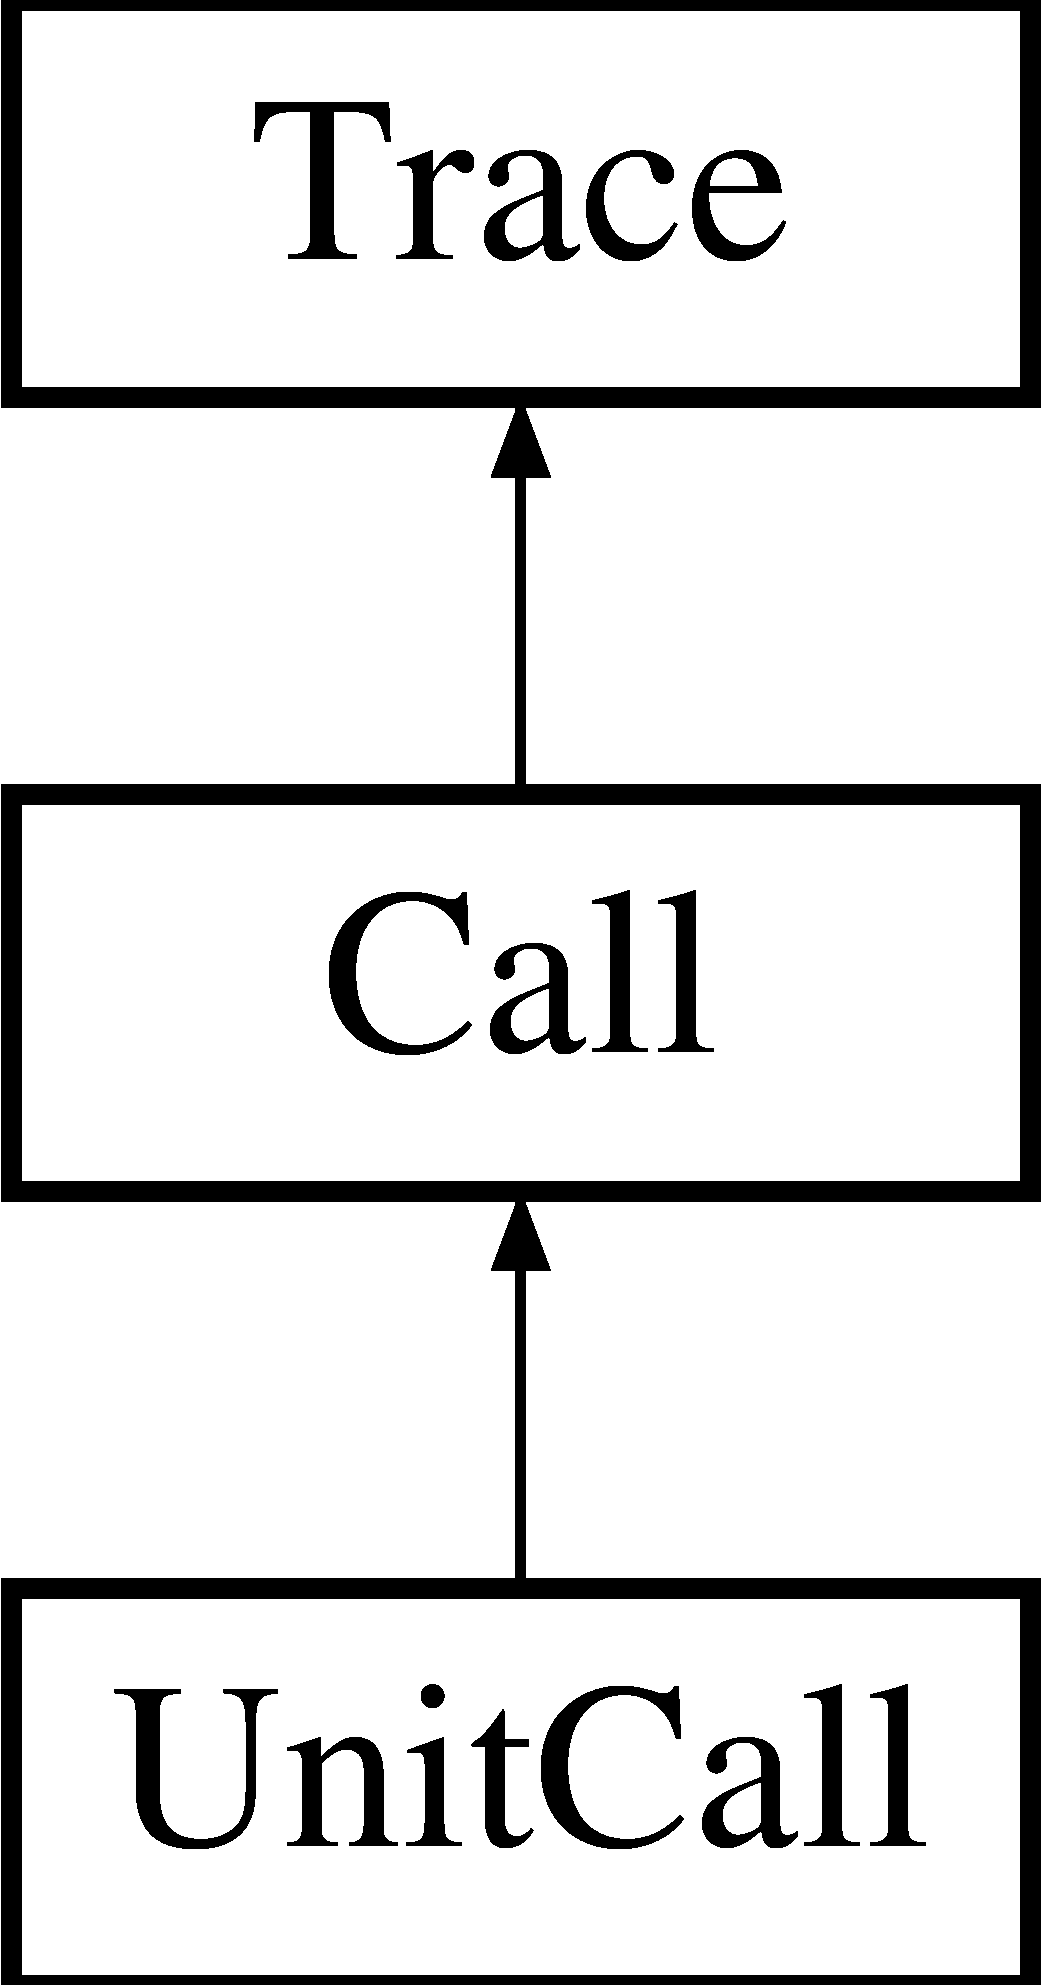
\includegraphics[height=3.000000cm]{class_unit_call}
\end{center}
\end{figure}
\subsection*{Public Member Functions}
\begin{DoxyCompactItemize}
\item 
\hyperlink{class_unit_call_ad81db95c527471acbfe40dd2f6b06713}{Unit\+Call} (\hyperlink{class_call_ade833a08ce215aaa4121102f3448c898}{Error\+Type} \hyperlink{class_call_a206f6150a8038fda48c17c2c7421aed1}{error}, std\+::string \hyperlink{class_call_ad6b8343d530798fdb48407b3f2489ae7}{label}, int unit\+Id, int unit\+Type)
\item 
\hyperlink{class_unit_call_a45ff0aedc68def7b44cb4c83252c298c}{Unit\+Call} (const \hyperlink{class_unit_call}{Unit\+Call} $\ast$c)
\item 
virtual \hyperlink{class_trace_a9c58e523529fc8a03fb6acf3eef86150}{Trace\+::sp\+\_\+trace} \hyperlink{class_unit_call_a637d309cd3d0bc05849aa7ca20eb5f89}{clone} () const 
\begin{DoxyCompactList}\small\item\em Clonage d\textquotesingle{}un appel. \end{DoxyCompactList}\end{DoxyCompactItemize}
\subsection*{Additional Inherited Members}


\subsection{Detailed Description}


Definition at line 341 of file Call\+Def.\+h.



\subsection{Constructor \& Destructor Documentation}
\index{Unit\+Call@{Unit\+Call}!Unit\+Call@{Unit\+Call}}
\index{Unit\+Call@{Unit\+Call}!Unit\+Call@{Unit\+Call}}
\subsubsection[{\texorpdfstring{Unit\+Call(\+Error\+Type error, std\+::string label, int unit\+Id, int unit\+Type)}{UnitCall(ErrorType error, std::string label, int unitId, int unitType)}}]{\setlength{\rightskip}{0pt plus 5cm}Unit\+Call\+::\+Unit\+Call (
\begin{DoxyParamCaption}
\item[{{\bf Error\+Type}}]{error, }
\item[{std\+::string}]{label, }
\item[{int}]{unit\+Id, }
\item[{int}]{unit\+Type}
\end{DoxyParamCaption}
)\hspace{0.3cm}{\ttfamily [inline]}}\hypertarget{class_unit_call_ad81db95c527471acbfe40dd2f6b06713}{}\label{class_unit_call_ad81db95c527471acbfe40dd2f6b06713}


Definition at line 345 of file Call\+Def.\+h.

\index{Unit\+Call@{Unit\+Call}!Unit\+Call@{Unit\+Call}}
\index{Unit\+Call@{Unit\+Call}!Unit\+Call@{Unit\+Call}}
\subsubsection[{\texorpdfstring{Unit\+Call(const Unit\+Call $\ast$c)}{UnitCall(const UnitCall *c)}}]{\setlength{\rightskip}{0pt plus 5cm}Unit\+Call\+::\+Unit\+Call (
\begin{DoxyParamCaption}
\item[{const {\bf Unit\+Call} $\ast$}]{c}
\end{DoxyParamCaption}
)\hspace{0.3cm}{\ttfamily [inline]}}\hypertarget{class_unit_call_a45ff0aedc68def7b44cb4c83252c298c}{}\label{class_unit_call_a45ff0aedc68def7b44cb4c83252c298c}


Definition at line 350 of file Call\+Def.\+h.



\subsection{Member Function Documentation}
\index{Unit\+Call@{Unit\+Call}!clone@{clone}}
\index{clone@{clone}!Unit\+Call@{Unit\+Call}}
\subsubsection[{\texorpdfstring{clone() const }{clone() const }}]{\setlength{\rightskip}{0pt plus 5cm}virtual {\bf Trace\+::sp\+\_\+trace} Unit\+Call\+::clone (
\begin{DoxyParamCaption}
{}
\end{DoxyParamCaption}
) const\hspace{0.3cm}{\ttfamily [inline]}, {\ttfamily [virtual]}}\hypertarget{class_unit_call_a637d309cd3d0bc05849aa7ca20eb5f89}{}\label{class_unit_call_a637d309cd3d0bc05849aa7ca20eb5f89}


Clonage d\textquotesingle{}un appel. 

\begin{DoxyReturn}{Returns}
une copie de l\textquotesingle{}objet \hyperlink{class_call}{Call}. 
\end{DoxyReturn}


Implements \hyperlink{class_call_ab3bf0965d35eb1e97ecddaf2d3978e9b}{Call}.



Definition at line 355 of file Call\+Def.\+h.



The documentation for this class was generated from the following file\+:\begin{DoxyCompactItemize}
\item 
C\+:/\+Users/\+Stephane/\+Desktop/mocahteam/\+Prog\+And\+Play/pp/traces/src/\hyperlink{_call_def_8h}{Call\+Def.\+h}\end{DoxyCompactItemize}

\hypertarget{class_untargeted_action_call}{}\section{Untargeted\+Action\+Call Class Reference}
\label{class_untargeted_action_call}\index{Untargeted\+Action\+Call@{Untargeted\+Action\+Call}}


{\ttfamily \#include $<$Call\+Def.\+h$>$}

Inheritance diagram for Untargeted\+Action\+Call\+:\begin{figure}[H]
\begin{center}
\leavevmode
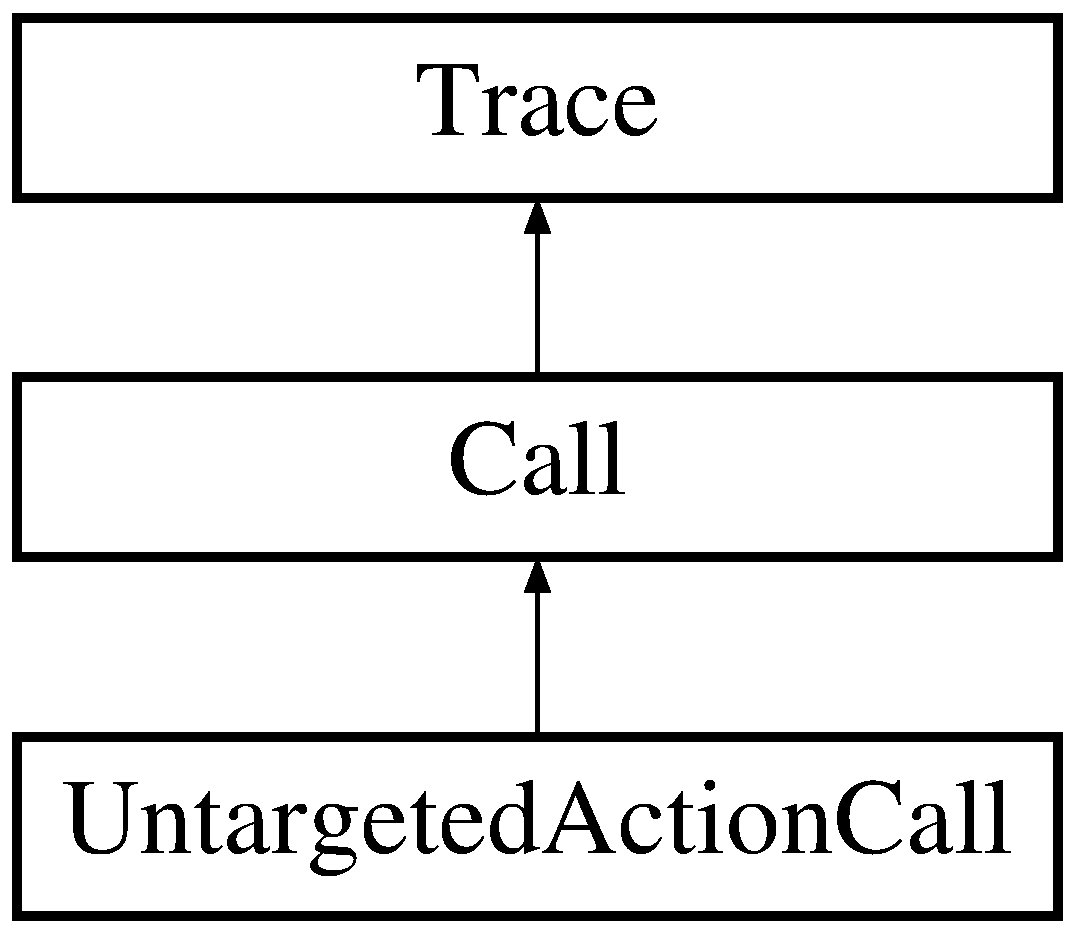
\includegraphics[height=3.000000cm]{class_untargeted_action_call}
\end{center}
\end{figure}
\subsection*{Public Member Functions}
\begin{DoxyCompactItemize}
\item 
\hyperlink{class_untargeted_action_call_aef6fd05ef0cab0c062feb64967e3e7c2}{Untargeted\+Action\+Call} (\hyperlink{class_call_ade833a08ce215aaa4121102f3448c898}{Error\+Type} \hyperlink{class_call_a206f6150a8038fda48c17c2c7421aed1}{error}, int unit\+Id, int unit\+Type, int action, float param)
\item 
\hyperlink{class_untargeted_action_call_ae888d621e1616e1e6a4aa427f1e5b2d5}{Untargeted\+Action\+Call} (const \hyperlink{class_untargeted_action_call}{Untargeted\+Action\+Call} $\ast$c)
\item 
virtual \hyperlink{class_trace_a9c58e523529fc8a03fb6acf3eef86150}{Trace\+::sp\+\_\+trace} \hyperlink{class_untargeted_action_call_a483d86c01a984c4b1e59e339a1f7329e}{clone} () const 
\begin{DoxyCompactList}\small\item\em Clonage d\textquotesingle{}un appel. \end{DoxyCompactList}\end{DoxyCompactItemize}
\subsection*{Additional Inherited Members}


\subsection{Detailed Description}


Definition at line 703 of file Call\+Def.\+h.



\subsection{Constructor \& Destructor Documentation}
\index{Untargeted\+Action\+Call@{Untargeted\+Action\+Call}!Untargeted\+Action\+Call@{Untargeted\+Action\+Call}}
\index{Untargeted\+Action\+Call@{Untargeted\+Action\+Call}!Untargeted\+Action\+Call@{Untargeted\+Action\+Call}}
\subsubsection[{\texorpdfstring{Untargeted\+Action\+Call(\+Error\+Type error, int unit\+Id, int unit\+Type, int action, float param)}{UntargetedActionCall(ErrorType error, int unitId, int unitType, int action, float param)}}]{\setlength{\rightskip}{0pt plus 5cm}Untargeted\+Action\+Call\+::\+Untargeted\+Action\+Call (
\begin{DoxyParamCaption}
\item[{{\bf Error\+Type}}]{error, }
\item[{int}]{unit\+Id, }
\item[{int}]{unit\+Type, }
\item[{int}]{action, }
\item[{float}]{param}
\end{DoxyParamCaption}
)\hspace{0.3cm}{\ttfamily [inline]}}\hypertarget{class_untargeted_action_call_aef6fd05ef0cab0c062feb64967e3e7c2}{}\label{class_untargeted_action_call_aef6fd05ef0cab0c062feb64967e3e7c2}


Definition at line 707 of file Call\+Def.\+h.

\index{Untargeted\+Action\+Call@{Untargeted\+Action\+Call}!Untargeted\+Action\+Call@{Untargeted\+Action\+Call}}
\index{Untargeted\+Action\+Call@{Untargeted\+Action\+Call}!Untargeted\+Action\+Call@{Untargeted\+Action\+Call}}
\subsubsection[{\texorpdfstring{Untargeted\+Action\+Call(const Untargeted\+Action\+Call $\ast$c)}{UntargetedActionCall(const UntargetedActionCall *c)}}]{\setlength{\rightskip}{0pt plus 5cm}Untargeted\+Action\+Call\+::\+Untargeted\+Action\+Call (
\begin{DoxyParamCaption}
\item[{const {\bf Untargeted\+Action\+Call} $\ast$}]{c}
\end{DoxyParamCaption}
)\hspace{0.3cm}{\ttfamily [inline]}}\hypertarget{class_untargeted_action_call_ae888d621e1616e1e6a4aa427f1e5b2d5}{}\label{class_untargeted_action_call_ae888d621e1616e1e6a4aa427f1e5b2d5}


Definition at line 712 of file Call\+Def.\+h.



\subsection{Member Function Documentation}
\index{Untargeted\+Action\+Call@{Untargeted\+Action\+Call}!clone@{clone}}
\index{clone@{clone}!Untargeted\+Action\+Call@{Untargeted\+Action\+Call}}
\subsubsection[{\texorpdfstring{clone() const }{clone() const }}]{\setlength{\rightskip}{0pt plus 5cm}virtual {\bf Trace\+::sp\+\_\+trace} Untargeted\+Action\+Call\+::clone (
\begin{DoxyParamCaption}
{}
\end{DoxyParamCaption}
) const\hspace{0.3cm}{\ttfamily [inline]}, {\ttfamily [virtual]}}\hypertarget{class_untargeted_action_call_a483d86c01a984c4b1e59e339a1f7329e}{}\label{class_untargeted_action_call_a483d86c01a984c4b1e59e339a1f7329e}


Clonage d\textquotesingle{}un appel. 

\begin{DoxyReturn}{Returns}
une copie de l\textquotesingle{}objet \hyperlink{class_call}{Call}. 
\end{DoxyReturn}


Implements \hyperlink{class_call_ab3bf0965d35eb1e97ecddaf2d3978e9b}{Call}.



Definition at line 719 of file Call\+Def.\+h.



The documentation for this class was generated from the following file\+:\begin{DoxyCompactItemize}
\item 
C\+:/\+Users/\+Stephane/\+Desktop/mocahteam/\+Prog\+And\+Play/pp/traces/src/\hyperlink{_call_def_8h}{Call\+Def.\+h}\end{DoxyCompactItemize}

\chapter{File Documentation}
\hypertarget{_call_8cpp}{}\section{C\+:/\+Users/\+Stephane/\+Desktop/mocahteam/\+Prog\+And\+Play/pp/traces/src/\+Call.cpp File Reference}
\label{_call_8cpp}\index{C\+:/\+Users/\+Stephane/\+Desktop/mocahteam/\+Prog\+And\+Play/pp/traces/src/\+Call.\+cpp@{C\+:/\+Users/\+Stephane/\+Desktop/mocahteam/\+Prog\+And\+Play/pp/traces/src/\+Call.\+cpp}}
{\ttfamily \#include \char`\"{}Call.\+h\char`\"{}}\\*

\hypertarget{_call_8h}{}\section{C\+:/\+Users/\+Stephane/\+Desktop/mocahteam/\+Prog\+And\+Play/pp/traces/src/\+Call.h File Reference}
\label{_call_8h}\index{C\+:/\+Users/\+Stephane/\+Desktop/mocahteam/\+Prog\+And\+Play/pp/traces/src/\+Call.\+h@{C\+:/\+Users/\+Stephane/\+Desktop/mocahteam/\+Prog\+And\+Play/pp/traces/src/\+Call.\+h}}


Déclaration des classes \hyperlink{class_call}{Call} et \hyperlink{class_params_map}{Params\+Map}.  


{\ttfamily \#include $<$iostream$>$}\\*
{\ttfamily \#include $<$fstream$>$}\\*
{\ttfamily \#include $<$sstream$>$}\\*
{\ttfamily \#include $<$map$>$}\\*
{\ttfamily \#include $<$vector$>$}\\*
{\ttfamily \#include $<$algorithm$>$}\\*
{\ttfamily \#include $<$stdexcept$>$}\\*
{\ttfamily \#include $<$rapidjson/document.\+h$>$}\\*
{\ttfamily \#include $<$boost/lexical\+\_\+cast.\+hpp$>$}\\*
{\ttfamily \#include \char`\"{}Trace.\+h\char`\"{}}\\*
\subsection*{Classes}
\begin{DoxyCompactItemize}
\item 
class \hyperlink{class_params_map}{Params\+Map}
\begin{DoxyCompactList}\small\item\em Classe utilisée pour le chargement des paramètres de compression à partir du fichier J\+S\+ON \textquotesingle{}params.\+json\textquotesingle{}. \end{DoxyCompactList}\item 
class \hyperlink{class_call}{Call}
\begin{DoxyCompactList}\small\item\em Classe abstraite héritant de \hyperlink{class_trace}{Trace}. Cette classe sert de classe mère pour toutes les classes définies dans le fichier \hyperlink{_call_def_8h}{Call\+Def.\+h}. \end{DoxyCompactList}\end{DoxyCompactItemize}
\subsection*{Macros}
\begin{DoxyCompactItemize}
\item 
\#define \hyperlink{_call_8h_a92280872d50a2c64ffe1acbc6c88dfff}{M\+A\+X\+\_\+\+S\+I\+Z\+E\+\_\+\+P\+A\+R\+A\+MS}~2
\item 
\#define \hyperlink{_call_8h_a4b857c8e2ae4074d043871fd75adfcef}{D\+E\+F\+A\+U\+L\+T\+\_\+\+C\+O\+M\+P\+R\+E\+S\+S\+I\+O\+N\+\_\+\+M\+OD}~0
\end{DoxyCompactItemize}


\subsection{Detailed Description}
Déclaration des classes \hyperlink{class_call}{Call} et \hyperlink{class_params_map}{Params\+Map}. 

\begin{DoxyAuthor}{Author}
meresse 
\end{DoxyAuthor}
\begin{DoxyVersion}{Version}
0.\+1 
\end{DoxyVersion}


\subsection{Macro Definition Documentation}
\index{Call.\+h@{Call.\+h}!D\+E\+F\+A\+U\+L\+T\+\_\+\+C\+O\+M\+P\+R\+E\+S\+S\+I\+O\+N\+\_\+\+M\+OD@{D\+E\+F\+A\+U\+L\+T\+\_\+\+C\+O\+M\+P\+R\+E\+S\+S\+I\+O\+N\+\_\+\+M\+OD}}
\index{D\+E\+F\+A\+U\+L\+T\+\_\+\+C\+O\+M\+P\+R\+E\+S\+S\+I\+O\+N\+\_\+\+M\+OD@{D\+E\+F\+A\+U\+L\+T\+\_\+\+C\+O\+M\+P\+R\+E\+S\+S\+I\+O\+N\+\_\+\+M\+OD}!Call.\+h@{Call.\+h}}
\subsubsection[{\texorpdfstring{D\+E\+F\+A\+U\+L\+T\+\_\+\+C\+O\+M\+P\+R\+E\+S\+S\+I\+O\+N\+\_\+\+M\+OD}{DEFAULT_COMPRESSION_MOD}}]{\setlength{\rightskip}{0pt plus 5cm}\#define D\+E\+F\+A\+U\+L\+T\+\_\+\+C\+O\+M\+P\+R\+E\+S\+S\+I\+O\+N\+\_\+\+M\+OD~0}\hypertarget{_call_8h_a4b857c8e2ae4074d043871fd75adfcef}{}\label{_call_8h_a4b857c8e2ae4074d043871fd75adfcef}
si D\+E\+F\+A\+U\+L\+T\+\_\+\+C\+O\+M\+P\+R\+E\+S\+S\+I\+O\+N\+\_\+\+M\+OD == 0, alors aucune valeur de paramètre n\textquotesingle{}est utilisé durant la compression. Sinon, tous les paramètres sont pris en compte pour la compression. 

Definition at line 28 of file Call.\+h.

\index{Call.\+h@{Call.\+h}!M\+A\+X\+\_\+\+S\+I\+Z\+E\+\_\+\+P\+A\+R\+A\+MS@{M\+A\+X\+\_\+\+S\+I\+Z\+E\+\_\+\+P\+A\+R\+A\+MS}}
\index{M\+A\+X\+\_\+\+S\+I\+Z\+E\+\_\+\+P\+A\+R\+A\+MS@{M\+A\+X\+\_\+\+S\+I\+Z\+E\+\_\+\+P\+A\+R\+A\+MS}!Call.\+h@{Call.\+h}}
\subsubsection[{\texorpdfstring{M\+A\+X\+\_\+\+S\+I\+Z\+E\+\_\+\+P\+A\+R\+A\+MS}{MAX_SIZE_PARAMS}}]{\setlength{\rightskip}{0pt plus 5cm}\#define M\+A\+X\+\_\+\+S\+I\+Z\+E\+\_\+\+P\+A\+R\+A\+MS~2}\hypertarget{_call_8h_a92280872d50a2c64ffe1acbc6c88dfff}{}\label{_call_8h_a92280872d50a2c64ffe1acbc6c88dfff}


Definition at line 11 of file Call.\+h.


\hypertarget{_call_def_8h}{}\section{C\+:/\+Users/\+Stephane/\+Desktop/mocahteam/\+Prog\+And\+Play/pp/traces/src/\+Call\+Def.h File Reference}
\label{_call_def_8h}\index{C\+:/\+Users/\+Stephane/\+Desktop/mocahteam/\+Prog\+And\+Play/pp/traces/src/\+Call\+Def.\+h@{C\+:/\+Users/\+Stephane/\+Desktop/mocahteam/\+Prog\+And\+Play/pp/traces/src/\+Call\+Def.\+h}}


Déclaration des classes dérivées de la classe \hyperlink{class_call}{Call}.  


{\ttfamily \#include $<$cmath$>$}\\*
{\ttfamily \#include $<$boost/lexical\+\_\+cast.\+hpp$>$}\\*
{\ttfamily \#include \char`\"{}Call.\+h\char`\"{}}\\*
{\ttfamily \#include \char`\"{}Traces\+Analyser.\+h\char`\"{}}\\*
\subsection*{Classes}
\begin{DoxyCompactItemize}
\item 
struct \hyperlink{struct_call_misc_1_1_unit}{Call\+Misc\+::\+Unit}
\item 
struct \hyperlink{struct_call_misc_1_1_position}{Call\+Misc\+::\+Position}
\item 
class \hyperlink{class_no_param_call}{No\+Param\+Call}
\item 
class \hyperlink{class_get_special_area_position_call}{Get\+Special\+Area\+Position\+Call}
\item 
class \hyperlink{class_get_resource_call}{Get\+Resource\+Call}
\item 
class \hyperlink{class_get_num_units_call}{Get\+Num\+Units\+Call}
\item 
class \hyperlink{class_get_unit_at_call}{Get\+Unit\+At\+Call}
\item 
class \hyperlink{class_unit_call}{Unit\+Call}
\item 
class \hyperlink{class_set_group_call}{Set\+Group\+Call}
\item 
class \hyperlink{class_action_on_unit_call}{Action\+On\+Unit\+Call}
\item 
class \hyperlink{class_action_on_position_call}{Action\+On\+Position\+Call}
\item 
class \hyperlink{class_untargeted_action_call}{Untargeted\+Action\+Call}
\item 
class \hyperlink{class_get_code_pdg_cmd_call}{Get\+Code\+Pdg\+Cmd\+Call}
\item 
class \hyperlink{class_get_num_params_pdg_cmd_call}{Get\+Num\+Params\+Pdg\+Cmd\+Call}
\item 
class \hyperlink{class_get_param_pdg_cmd_call}{Get\+Param\+Pdg\+Cmd\+Call}
\end{DoxyCompactItemize}
\subsection*{Namespaces}
\begin{DoxyCompactItemize}
\item 
 \hyperlink{namespace_call_misc}{Call\+Misc}
\end{DoxyCompactItemize}
\subsection*{Enumerations}
\begin{DoxyCompactItemize}
\item 
enum \hyperlink{namespace_call_misc_a490b3c2ef1a821675848ebcab0b677d8}{Call\+Misc\+::\+Coalition} \{ \hyperlink{namespace_call_misc_a490b3c2ef1a821675848ebcab0b677d8a55c17878e61b97e8ce25f6dc4c2da627}{Call\+Misc\+::\+N\+O\+NE} = -\/1, 
\hyperlink{namespace_call_misc_a490b3c2ef1a821675848ebcab0b677d8a38d26e9fc963014a8b85324685b853fc}{Call\+Misc\+::\+M\+Y\+\_\+\+C\+O\+A\+L\+I\+T\+I\+ON}, 
\hyperlink{namespace_call_misc_a490b3c2ef1a821675848ebcab0b677d8a6fc0ad3a442b6b9629c67957b12d1351}{Call\+Misc\+::\+A\+L\+L\+Y\+\_\+\+C\+O\+A\+L\+I\+T\+I\+ON}, 
\hyperlink{namespace_call_misc_a490b3c2ef1a821675848ebcab0b677d8a5b0cc8b822bdf2bab495983dcd24a4e4}{Call\+Misc\+::\+E\+N\+E\+M\+Y\+\_\+\+C\+O\+A\+L\+I\+T\+I\+ON}
 \}
\end{DoxyCompactItemize}


\subsection{Detailed Description}
Déclaration des classes dérivées de la classe \hyperlink{class_call}{Call}. 

\begin{DoxyAuthor}{Author}
meresse 
\end{DoxyAuthor}
\begin{DoxyVersion}{Version}
0.\+1 
\end{DoxyVersion}

\hypertarget{constant_list___k_p4_84_8h}{}\section{C\+:/\+Users/\+Stephane/\+Desktop/mocahteam/\+Prog\+And\+Play/pp/traces/src/constant\+List\+\_\+\+K\+P4.4.h File Reference}
\label{constant_list___k_p4_84_8h}\index{C\+:/\+Users/\+Stephane/\+Desktop/mocahteam/\+Prog\+And\+Play/pp/traces/src/constant\+List\+\_\+\+K\+P4.\+4.\+h@{C\+:/\+Users/\+Stephane/\+Desktop/mocahteam/\+Prog\+And\+Play/pp/traces/src/constant\+List\+\_\+\+K\+P4.\+4.\+h}}
\subsection*{Macros}
\begin{DoxyCompactItemize}
\item 
\#define \hyperlink{constant_list___k_p4_84_8h_ae8c5bd8c5f093380079a69f65a92c7b8}{A\+S\+S\+E\+M\+B\+L\+ER}~2
\item 
\#define \hyperlink{constant_list___k_p4_84_8h_a9eadfc474fbb06e749b599eb1aaaa4ee}{B\+A\+D\+B\+L\+O\+CK}~3
\item 
\#define \hyperlink{constant_list___k_p4_84_8h_a7b846473f310e6962ca8b763772cf862}{B\+IT}~4
\item 
\#define \hyperlink{constant_list___k_p4_84_8h_aec93e83855ac17c3c25c55c37ca186dd}{B\+Y\+TE}~7
\item 
\#define \hyperlink{constant_list___k_p4_84_8h_ac4e52c1bd876037cd22e859f38fd5d27}{K\+E\+R\+N\+EL}~25
\item 
\#define \hyperlink{constant_list___k_p4_84_8h_a10217dfd84d85c7f8065a1f81068530a}{L\+O\+G\+I\+C\+\_\+\+B\+O\+MB}~26
\item 
\#define \hyperlink{constant_list___k_p4_84_8h_a84def408d1c5413e2c1d7fe9eeb18f09}{P\+O\+I\+N\+T\+ER}~39
\item 
\#define \hyperlink{constant_list___k_p4_84_8h_a4688695205ef66fbf096f1b95a0d7fe9}{S\+I\+G\+N\+AL}~44
\item 
\#define \hyperlink{constant_list___k_p4_84_8h_aff55fe551a9992a54ec54621c524d0a4}{S\+O\+C\+K\+ET}~45
\item 
\#define \hyperlink{constant_list___k_p4_84_8h_a5250b667cb28dd60b71e6e04e23eac37}{T\+E\+R\+M\+I\+N\+AL}~46
\item 
\#define \hyperlink{constant_list___k_p4_84_8h_ae19b6bb2940d2fbe0a79852b070eeafd}{S\+T\+OP}~0     /$\ast$ expect 0 parameters $\ast$/
\item 
\#define \hyperlink{constant_list___k_p4_84_8h_aef72fe86b7c60b1a86920496456edeac}{W\+A\+IT}~5     /$\ast$ expect 0 parameters $\ast$/
\item 
\#define \hyperlink{constant_list___k_p4_84_8h_a549849b55e689f3972aeef6c0a8a23aa}{F\+I\+R\+E\+\_\+\+S\+T\+A\+TE}
\item 
\#define \hyperlink{constant_list___k_p4_84_8h_a5ed231278f33db1b399ada4cdb5ab8b3}{S\+E\+L\+F\+\_\+\+D\+E\+S\+T\+R\+U\+C\+T\+I\+ON}~65    /$\ast$ expect 0 parameters $\ast$/
\item 
\#define \hyperlink{constant_list___k_p4_84_8h_a2c9384c67919c632913b8db2088f8341}{R\+E\+P\+E\+AT}
\item 
\#define \hyperlink{constant_list___k_p4_84_8h_a2acdc4aa0f128c9b2788707db3e6935e}{M\+O\+VE}~10    /$\ast$ expect 1 parameter\+: a position or a unit $\ast$/
\item 
\#define \hyperlink{constant_list___k_p4_84_8h_a8ba7f54b1db5078f0193a9f2109cb402}{P\+A\+T\+R\+OL}~15    /$\ast$ expect 1 parameter\+: a position or a unit $\ast$/
\item 
\#define \hyperlink{constant_list___k_p4_84_8h_a7f0f49f349d8a6d2e1660672cd1f3445}{F\+I\+G\+HT}~16    /$\ast$ expect 1 parameter\+: a position or a unit $\ast$/
\item 
\#define \hyperlink{constant_list___k_p4_84_8h_a00f4bd52f68e818e8eb542ff64067f38}{G\+U\+A\+RD}~25    /$\ast$ expect 1 parameter\+: a position or a unit $\ast$/
\item 
\#define \hyperlink{constant_list___k_p4_84_8h_a8eefa9e0bf85e1a181fe2499ed84e6c4}{M\+O\+V\+E\+\_\+\+S\+T\+A\+TE}
\item 
\#define \hyperlink{constant_list___k_p4_84_8h_a65a3dd797f558f8b5388cf96aca94e5d}{A\+T\+T\+A\+CK}~20    /$\ast$ expect 1 parameter\+: a position or a unit $\ast$/
\item 
\#define \hyperlink{constant_list___k_p4_84_8h_aef41188f4525e5fad838815ca9251072}{R\+E\+P\+A\+IR}~40    /$\ast$ expect 1 parameter\+: a position or a unit $\ast$/
\item 
\#define \hyperlink{constant_list___k_p4_84_8h_ad1bc13a36f332a2a857966d777da9b2d}{R\+E\+C\+L\+A\+IM}~90    /$\ast$ expect 1 parameter\+: a position or a unit $\ast$/
\item 
\#define \hyperlink{constant_list___k_p4_84_8h_acd2ea0453b6daf41446e84a9f24a2e83}{R\+E\+S\+T\+O\+RE}~110   /$\ast$ expect 1 parameter\+: a position or a unit $\ast$/
\item 
\#define \hyperlink{constant_list___k_p4_84_8h_aefc84e18558515c7f94b3ee2c4c196d4}{B\+U\+I\+L\+D\+\_\+\+B\+A\+D\+B\+L\+O\+CK}~-\/3    /$\ast$ expect 1 parameter\+: a position or a unit $\ast$/
\item 
\#define \hyperlink{constant_list___k_p4_84_8h_a34af57b9e7bd2e9f0c773eef4c526adb}{B\+U\+I\+L\+D\+\_\+\+L\+O\+G\+I\+C\+\_\+\+B\+O\+MB}~-\/26   /$\ast$ expect 1 parameter\+: a position or a unit $\ast$/
\item 
\#define \hyperlink{constant_list___k_p4_84_8h_a293094523dc956fcd7ab4264fff51047}{B\+U\+I\+L\+D\+\_\+\+S\+O\+C\+K\+ET}~-\/45   /$\ast$ expect 1 parameter\+: a position or a unit $\ast$/
\item 
\#define \hyperlink{constant_list___k_p4_84_8h_aaee336bdf6720e7a7704d8a49f4b4cbc}{B\+U\+I\+L\+D\+\_\+\+T\+E\+R\+M\+I\+N\+AL}~-\/46   /$\ast$ expect 1 parameter\+: a position or a unit $\ast$/
\item 
\#define \hyperlink{constant_list___k_p4_84_8h_ad72dbcf6d0153db1b8d8a58001feed83}{D\+E\+B\+UG}~-\/35   /$\ast$ expect 1 parameter\+: a position or a unit $\ast$/
\item 
\#define \hyperlink{constant_list___k_p4_84_8h_af9806d63a68bdbdb3b8accfe0a2dcf00}{B\+U\+I\+L\+D\+\_\+\+A\+S\+S\+E\+M\+B\+L\+ER}~-\/2    /$\ast$ expect 1 parameter\+: a position or a unit $\ast$/
\item 
\#define \hyperlink{constant_list___k_p4_84_8h_aa2c9def3b7bb224a9427fb4d04f8ef61}{B\+U\+I\+L\+D\+\_\+\+B\+Y\+TE}~-\/7    /$\ast$ expect 1 parameter\+: a position or a unit $\ast$/
\item 
\#define \hyperlink{constant_list___k_p4_84_8h_aa700fcae761fc903fb17e0c922a2ad41}{B\+U\+I\+L\+D\+\_\+\+P\+O\+I\+N\+T\+ER}~-\/39   /$\ast$ expect 1 parameter\+: a position or a unit $\ast$/
\item 
\#define \hyperlink{constant_list___k_p4_84_8h_a3a37118e05389462481249cec2e67b8d}{B\+U\+I\+L\+D\+\_\+\+B\+IT}~-\/4    /$\ast$ expect 1 parameter\+: a position or a unit $\ast$/
\item 
\#define \hyperlink{constant_list___k_p4_84_8h_a20b8248964dd31f9ce2d83b3c0630d79}{S\+T\+O\+P\+\_\+\+B\+U\+I\+L\+D\+I\+NG}~-\/7658 /$\ast$ expect 0 parameters $\ast$/
\item 
\#define \hyperlink{constant_list___k_p4_84_8h_a54dd54e46d425790a3e7380bd54b7788}{L\+A\+U\+N\+C\+H\+\_\+\+M\+I\+NE}~33395 /$\ast$ expect 0 parameters $\ast$/
\item 
\#define \hyperlink{constant_list___k_p4_84_8h_a7c16ee2e7cb0fb0132818a1bce15bbe7}{N\+X\+\_\+\+F\+L\+AG}~33389 /$\ast$ expect 1 parameter\+: a position or a unit $\ast$/
\item 
\#define \hyperlink{constant_list___k_p4_84_8h_a682182a5e5f38fd61f4311501e9dac5d}{S\+I\+G\+T\+E\+RM}~35126 /$\ast$ expect 1 parameter\+: a position or a unit $\ast$/
\item 
\#define \hyperlink{constant_list___k_p4_84_8h_aaf564f552d81c136a77e3a60b1a8ccfc}{M\+E\+T\+AL}~0
\item 
\#define \hyperlink{constant_list___k_p4_84_8h_abfeccb70507156fe545bf4dfc1b3f0c1}{E\+N\+E\+R\+GY}~1
\end{DoxyCompactItemize}


\subsection{Macro Definition Documentation}
\index{constant\+List\+\_\+\+K\+P4.\+4.\+h@{constant\+List\+\_\+\+K\+P4.\+4.\+h}!A\+S\+S\+E\+M\+B\+L\+ER@{A\+S\+S\+E\+M\+B\+L\+ER}}
\index{A\+S\+S\+E\+M\+B\+L\+ER@{A\+S\+S\+E\+M\+B\+L\+ER}!constant\+List\+\_\+\+K\+P4.\+4.\+h@{constant\+List\+\_\+\+K\+P4.\+4.\+h}}
\subsubsection[{\texorpdfstring{A\+S\+S\+E\+M\+B\+L\+ER}{ASSEMBLER}}]{\setlength{\rightskip}{0pt plus 5cm}\#define A\+S\+S\+E\+M\+B\+L\+ER~2}\hypertarget{constant_list___k_p4_84_8h_ae8c5bd8c5f093380079a69f65a92c7b8}{}\label{constant_list___k_p4_84_8h_ae8c5bd8c5f093380079a69f65a92c7b8}


Definition at line 10 of file constant\+List\+\_\+\+K\+P4.\+4.\+h.

\index{constant\+List\+\_\+\+K\+P4.\+4.\+h@{constant\+List\+\_\+\+K\+P4.\+4.\+h}!A\+T\+T\+A\+CK@{A\+T\+T\+A\+CK}}
\index{A\+T\+T\+A\+CK@{A\+T\+T\+A\+CK}!constant\+List\+\_\+\+K\+P4.\+4.\+h@{constant\+List\+\_\+\+K\+P4.\+4.\+h}}
\subsubsection[{\texorpdfstring{A\+T\+T\+A\+CK}{ATTACK}}]{\setlength{\rightskip}{0pt plus 5cm}\#define A\+T\+T\+A\+CK~20    /$\ast$ expect 1 parameter\+: a position or a unit $\ast$/}\hypertarget{constant_list___k_p4_84_8h_a65a3dd797f558f8b5388cf96aca94e5d}{}\label{constant_list___k_p4_84_8h_a65a3dd797f558f8b5388cf96aca94e5d}


Definition at line 49 of file constant\+List\+\_\+\+K\+P4.\+4.\+h.

\index{constant\+List\+\_\+\+K\+P4.\+4.\+h@{constant\+List\+\_\+\+K\+P4.\+4.\+h}!B\+A\+D\+B\+L\+O\+CK@{B\+A\+D\+B\+L\+O\+CK}}
\index{B\+A\+D\+B\+L\+O\+CK@{B\+A\+D\+B\+L\+O\+CK}!constant\+List\+\_\+\+K\+P4.\+4.\+h@{constant\+List\+\_\+\+K\+P4.\+4.\+h}}
\subsubsection[{\texorpdfstring{B\+A\+D\+B\+L\+O\+CK}{BADBLOCK}}]{\setlength{\rightskip}{0pt plus 5cm}\#define B\+A\+D\+B\+L\+O\+CK~3}\hypertarget{constant_list___k_p4_84_8h_a9eadfc474fbb06e749b599eb1aaaa4ee}{}\label{constant_list___k_p4_84_8h_a9eadfc474fbb06e749b599eb1aaaa4ee}


Definition at line 11 of file constant\+List\+\_\+\+K\+P4.\+4.\+h.

\index{constant\+List\+\_\+\+K\+P4.\+4.\+h@{constant\+List\+\_\+\+K\+P4.\+4.\+h}!B\+IT@{B\+IT}}
\index{B\+IT@{B\+IT}!constant\+List\+\_\+\+K\+P4.\+4.\+h@{constant\+List\+\_\+\+K\+P4.\+4.\+h}}
\subsubsection[{\texorpdfstring{B\+IT}{BIT}}]{\setlength{\rightskip}{0pt plus 5cm}\#define B\+IT~4}\hypertarget{constant_list___k_p4_84_8h_a7b846473f310e6962ca8b763772cf862}{}\label{constant_list___k_p4_84_8h_a7b846473f310e6962ca8b763772cf862}


Definition at line 12 of file constant\+List\+\_\+\+K\+P4.\+4.\+h.

\index{constant\+List\+\_\+\+K\+P4.\+4.\+h@{constant\+List\+\_\+\+K\+P4.\+4.\+h}!B\+U\+I\+L\+D\+\_\+\+A\+S\+S\+E\+M\+B\+L\+ER@{B\+U\+I\+L\+D\+\_\+\+A\+S\+S\+E\+M\+B\+L\+ER}}
\index{B\+U\+I\+L\+D\+\_\+\+A\+S\+S\+E\+M\+B\+L\+ER@{B\+U\+I\+L\+D\+\_\+\+A\+S\+S\+E\+M\+B\+L\+ER}!constant\+List\+\_\+\+K\+P4.\+4.\+h@{constant\+List\+\_\+\+K\+P4.\+4.\+h}}
\subsubsection[{\texorpdfstring{B\+U\+I\+L\+D\+\_\+\+A\+S\+S\+E\+M\+B\+L\+ER}{BUILD_ASSEMBLER}}]{\setlength{\rightskip}{0pt plus 5cm}\#define B\+U\+I\+L\+D\+\_\+\+A\+S\+S\+E\+M\+B\+L\+ER~-\/2    /$\ast$ expect 1 parameter\+: a position or a unit $\ast$/}\hypertarget{constant_list___k_p4_84_8h_af9806d63a68bdbdb3b8accfe0a2dcf00}{}\label{constant_list___k_p4_84_8h_af9806d63a68bdbdb3b8accfe0a2dcf00}


Definition at line 64 of file constant\+List\+\_\+\+K\+P4.\+4.\+h.

\index{constant\+List\+\_\+\+K\+P4.\+4.\+h@{constant\+List\+\_\+\+K\+P4.\+4.\+h}!B\+U\+I\+L\+D\+\_\+\+B\+A\+D\+B\+L\+O\+CK@{B\+U\+I\+L\+D\+\_\+\+B\+A\+D\+B\+L\+O\+CK}}
\index{B\+U\+I\+L\+D\+\_\+\+B\+A\+D\+B\+L\+O\+CK@{B\+U\+I\+L\+D\+\_\+\+B\+A\+D\+B\+L\+O\+CK}!constant\+List\+\_\+\+K\+P4.\+4.\+h@{constant\+List\+\_\+\+K\+P4.\+4.\+h}}
\subsubsection[{\texorpdfstring{B\+U\+I\+L\+D\+\_\+\+B\+A\+D\+B\+L\+O\+CK}{BUILD_BADBLOCK}}]{\setlength{\rightskip}{0pt plus 5cm}\#define B\+U\+I\+L\+D\+\_\+\+B\+A\+D\+B\+L\+O\+CK~-\/3    /$\ast$ expect 1 parameter\+: a position or a unit $\ast$/}\hypertarget{constant_list___k_p4_84_8h_aefc84e18558515c7f94b3ee2c4c196d4}{}\label{constant_list___k_p4_84_8h_aefc84e18558515c7f94b3ee2c4c196d4}


Definition at line 56 of file constant\+List\+\_\+\+K\+P4.\+4.\+h.

\index{constant\+List\+\_\+\+K\+P4.\+4.\+h@{constant\+List\+\_\+\+K\+P4.\+4.\+h}!B\+U\+I\+L\+D\+\_\+\+B\+IT@{B\+U\+I\+L\+D\+\_\+\+B\+IT}}
\index{B\+U\+I\+L\+D\+\_\+\+B\+IT@{B\+U\+I\+L\+D\+\_\+\+B\+IT}!constant\+List\+\_\+\+K\+P4.\+4.\+h@{constant\+List\+\_\+\+K\+P4.\+4.\+h}}
\subsubsection[{\texorpdfstring{B\+U\+I\+L\+D\+\_\+\+B\+IT}{BUILD_BIT}}]{\setlength{\rightskip}{0pt plus 5cm}\#define B\+U\+I\+L\+D\+\_\+\+B\+IT~-\/4    /$\ast$ expect 1 parameter\+: a position or a unit $\ast$/}\hypertarget{constant_list___k_p4_84_8h_a3a37118e05389462481249cec2e67b8d}{}\label{constant_list___k_p4_84_8h_a3a37118e05389462481249cec2e67b8d}


Definition at line 70 of file constant\+List\+\_\+\+K\+P4.\+4.\+h.

\index{constant\+List\+\_\+\+K\+P4.\+4.\+h@{constant\+List\+\_\+\+K\+P4.\+4.\+h}!B\+U\+I\+L\+D\+\_\+\+B\+Y\+TE@{B\+U\+I\+L\+D\+\_\+\+B\+Y\+TE}}
\index{B\+U\+I\+L\+D\+\_\+\+B\+Y\+TE@{B\+U\+I\+L\+D\+\_\+\+B\+Y\+TE}!constant\+List\+\_\+\+K\+P4.\+4.\+h@{constant\+List\+\_\+\+K\+P4.\+4.\+h}}
\subsubsection[{\texorpdfstring{B\+U\+I\+L\+D\+\_\+\+B\+Y\+TE}{BUILD_BYTE}}]{\setlength{\rightskip}{0pt plus 5cm}\#define B\+U\+I\+L\+D\+\_\+\+B\+Y\+TE~-\/7    /$\ast$ expect 1 parameter\+: a position or a unit $\ast$/}\hypertarget{constant_list___k_p4_84_8h_aa2c9def3b7bb224a9427fb4d04f8ef61}{}\label{constant_list___k_p4_84_8h_aa2c9def3b7bb224a9427fb4d04f8ef61}


Definition at line 65 of file constant\+List\+\_\+\+K\+P4.\+4.\+h.

\index{constant\+List\+\_\+\+K\+P4.\+4.\+h@{constant\+List\+\_\+\+K\+P4.\+4.\+h}!B\+U\+I\+L\+D\+\_\+\+L\+O\+G\+I\+C\+\_\+\+B\+O\+MB@{B\+U\+I\+L\+D\+\_\+\+L\+O\+G\+I\+C\+\_\+\+B\+O\+MB}}
\index{B\+U\+I\+L\+D\+\_\+\+L\+O\+G\+I\+C\+\_\+\+B\+O\+MB@{B\+U\+I\+L\+D\+\_\+\+L\+O\+G\+I\+C\+\_\+\+B\+O\+MB}!constant\+List\+\_\+\+K\+P4.\+4.\+h@{constant\+List\+\_\+\+K\+P4.\+4.\+h}}
\subsubsection[{\texorpdfstring{B\+U\+I\+L\+D\+\_\+\+L\+O\+G\+I\+C\+\_\+\+B\+O\+MB}{BUILD_LOGIC_BOMB}}]{\setlength{\rightskip}{0pt plus 5cm}\#define B\+U\+I\+L\+D\+\_\+\+L\+O\+G\+I\+C\+\_\+\+B\+O\+MB~-\/26   /$\ast$ expect 1 parameter\+: a position or a unit $\ast$/}\hypertarget{constant_list___k_p4_84_8h_a34af57b9e7bd2e9f0c773eef4c526adb}{}\label{constant_list___k_p4_84_8h_a34af57b9e7bd2e9f0c773eef4c526adb}


Definition at line 57 of file constant\+List\+\_\+\+K\+P4.\+4.\+h.

\index{constant\+List\+\_\+\+K\+P4.\+4.\+h@{constant\+List\+\_\+\+K\+P4.\+4.\+h}!B\+U\+I\+L\+D\+\_\+\+P\+O\+I\+N\+T\+ER@{B\+U\+I\+L\+D\+\_\+\+P\+O\+I\+N\+T\+ER}}
\index{B\+U\+I\+L\+D\+\_\+\+P\+O\+I\+N\+T\+ER@{B\+U\+I\+L\+D\+\_\+\+P\+O\+I\+N\+T\+ER}!constant\+List\+\_\+\+K\+P4.\+4.\+h@{constant\+List\+\_\+\+K\+P4.\+4.\+h}}
\subsubsection[{\texorpdfstring{B\+U\+I\+L\+D\+\_\+\+P\+O\+I\+N\+T\+ER}{BUILD_POINTER}}]{\setlength{\rightskip}{0pt plus 5cm}\#define B\+U\+I\+L\+D\+\_\+\+P\+O\+I\+N\+T\+ER~-\/39   /$\ast$ expect 1 parameter\+: a position or a unit $\ast$/}\hypertarget{constant_list___k_p4_84_8h_aa700fcae761fc903fb17e0c922a2ad41}{}\label{constant_list___k_p4_84_8h_aa700fcae761fc903fb17e0c922a2ad41}


Definition at line 66 of file constant\+List\+\_\+\+K\+P4.\+4.\+h.

\index{constant\+List\+\_\+\+K\+P4.\+4.\+h@{constant\+List\+\_\+\+K\+P4.\+4.\+h}!B\+U\+I\+L\+D\+\_\+\+S\+O\+C\+K\+ET@{B\+U\+I\+L\+D\+\_\+\+S\+O\+C\+K\+ET}}
\index{B\+U\+I\+L\+D\+\_\+\+S\+O\+C\+K\+ET@{B\+U\+I\+L\+D\+\_\+\+S\+O\+C\+K\+ET}!constant\+List\+\_\+\+K\+P4.\+4.\+h@{constant\+List\+\_\+\+K\+P4.\+4.\+h}}
\subsubsection[{\texorpdfstring{B\+U\+I\+L\+D\+\_\+\+S\+O\+C\+K\+ET}{BUILD_SOCKET}}]{\setlength{\rightskip}{0pt plus 5cm}\#define B\+U\+I\+L\+D\+\_\+\+S\+O\+C\+K\+ET~-\/45   /$\ast$ expect 1 parameter\+: a position or a unit $\ast$/}\hypertarget{constant_list___k_p4_84_8h_a293094523dc956fcd7ab4264fff51047}{}\label{constant_list___k_p4_84_8h_a293094523dc956fcd7ab4264fff51047}


Definition at line 58 of file constant\+List\+\_\+\+K\+P4.\+4.\+h.

\index{constant\+List\+\_\+\+K\+P4.\+4.\+h@{constant\+List\+\_\+\+K\+P4.\+4.\+h}!B\+U\+I\+L\+D\+\_\+\+T\+E\+R\+M\+I\+N\+AL@{B\+U\+I\+L\+D\+\_\+\+T\+E\+R\+M\+I\+N\+AL}}
\index{B\+U\+I\+L\+D\+\_\+\+T\+E\+R\+M\+I\+N\+AL@{B\+U\+I\+L\+D\+\_\+\+T\+E\+R\+M\+I\+N\+AL}!constant\+List\+\_\+\+K\+P4.\+4.\+h@{constant\+List\+\_\+\+K\+P4.\+4.\+h}}
\subsubsection[{\texorpdfstring{B\+U\+I\+L\+D\+\_\+\+T\+E\+R\+M\+I\+N\+AL}{BUILD_TERMINAL}}]{\setlength{\rightskip}{0pt plus 5cm}\#define B\+U\+I\+L\+D\+\_\+\+T\+E\+R\+M\+I\+N\+AL~-\/46   /$\ast$ expect 1 parameter\+: a position or a unit $\ast$/}\hypertarget{constant_list___k_p4_84_8h_aaee336bdf6720e7a7704d8a49f4b4cbc}{}\label{constant_list___k_p4_84_8h_aaee336bdf6720e7a7704d8a49f4b4cbc}


Definition at line 59 of file constant\+List\+\_\+\+K\+P4.\+4.\+h.

\index{constant\+List\+\_\+\+K\+P4.\+4.\+h@{constant\+List\+\_\+\+K\+P4.\+4.\+h}!B\+Y\+TE@{B\+Y\+TE}}
\index{B\+Y\+TE@{B\+Y\+TE}!constant\+List\+\_\+\+K\+P4.\+4.\+h@{constant\+List\+\_\+\+K\+P4.\+4.\+h}}
\subsubsection[{\texorpdfstring{B\+Y\+TE}{BYTE}}]{\setlength{\rightskip}{0pt plus 5cm}\#define B\+Y\+TE~7}\hypertarget{constant_list___k_p4_84_8h_aec93e83855ac17c3c25c55c37ca186dd}{}\label{constant_list___k_p4_84_8h_aec93e83855ac17c3c25c55c37ca186dd}


Definition at line 13 of file constant\+List\+\_\+\+K\+P4.\+4.\+h.

\index{constant\+List\+\_\+\+K\+P4.\+4.\+h@{constant\+List\+\_\+\+K\+P4.\+4.\+h}!D\+E\+B\+UG@{D\+E\+B\+UG}}
\index{D\+E\+B\+UG@{D\+E\+B\+UG}!constant\+List\+\_\+\+K\+P4.\+4.\+h@{constant\+List\+\_\+\+K\+P4.\+4.\+h}}
\subsubsection[{\texorpdfstring{D\+E\+B\+UG}{DEBUG}}]{\setlength{\rightskip}{0pt plus 5cm}\#define D\+E\+B\+UG~-\/35   /$\ast$ expect 1 parameter\+: a position or a unit $\ast$/}\hypertarget{constant_list___k_p4_84_8h_ad72dbcf6d0153db1b8d8a58001feed83}{}\label{constant_list___k_p4_84_8h_ad72dbcf6d0153db1b8d8a58001feed83}


Definition at line 60 of file constant\+List\+\_\+\+K\+P4.\+4.\+h.

\index{constant\+List\+\_\+\+K\+P4.\+4.\+h@{constant\+List\+\_\+\+K\+P4.\+4.\+h}!E\+N\+E\+R\+GY@{E\+N\+E\+R\+GY}}
\index{E\+N\+E\+R\+GY@{E\+N\+E\+R\+GY}!constant\+List\+\_\+\+K\+P4.\+4.\+h@{constant\+List\+\_\+\+K\+P4.\+4.\+h}}
\subsubsection[{\texorpdfstring{E\+N\+E\+R\+GY}{ENERGY}}]{\setlength{\rightskip}{0pt plus 5cm}\#define E\+N\+E\+R\+GY~1}\hypertarget{constant_list___k_p4_84_8h_abfeccb70507156fe545bf4dfc1b3f0c1}{}\label{constant_list___k_p4_84_8h_abfeccb70507156fe545bf4dfc1b3f0c1}


Definition at line 89 of file constant\+List\+\_\+\+K\+P4.\+4.\+h.

\index{constant\+List\+\_\+\+K\+P4.\+4.\+h@{constant\+List\+\_\+\+K\+P4.\+4.\+h}!F\+I\+G\+HT@{F\+I\+G\+HT}}
\index{F\+I\+G\+HT@{F\+I\+G\+HT}!constant\+List\+\_\+\+K\+P4.\+4.\+h@{constant\+List\+\_\+\+K\+P4.\+4.\+h}}
\subsubsection[{\texorpdfstring{F\+I\+G\+HT}{FIGHT}}]{\setlength{\rightskip}{0pt plus 5cm}\#define F\+I\+G\+HT~16    /$\ast$ expect 1 parameter\+: a position or a unit $\ast$/}\hypertarget{constant_list___k_p4_84_8h_a7f0f49f349d8a6d2e1660672cd1f3445}{}\label{constant_list___k_p4_84_8h_a7f0f49f349d8a6d2e1660672cd1f3445}


Definition at line 40 of file constant\+List\+\_\+\+K\+P4.\+4.\+h.

\index{constant\+List\+\_\+\+K\+P4.\+4.\+h@{constant\+List\+\_\+\+K\+P4.\+4.\+h}!F\+I\+R\+E\+\_\+\+S\+T\+A\+TE@{F\+I\+R\+E\+\_\+\+S\+T\+A\+TE}}
\index{F\+I\+R\+E\+\_\+\+S\+T\+A\+TE@{F\+I\+R\+E\+\_\+\+S\+T\+A\+TE}!constant\+List\+\_\+\+K\+P4.\+4.\+h@{constant\+List\+\_\+\+K\+P4.\+4.\+h}}
\subsubsection[{\texorpdfstring{F\+I\+R\+E\+\_\+\+S\+T\+A\+TE}{FIRE_STATE}}]{\setlength{\rightskip}{0pt plus 5cm}\#define F\+I\+R\+E\+\_\+\+S\+T\+A\+TE}\hypertarget{constant_list___k_p4_84_8h_a549849b55e689f3972aeef6c0a8a23aa}{}\label{constant_list___k_p4_84_8h_a549849b55e689f3972aeef6c0a8a23aa}
{\bfseries Value\+:}
\begin{DoxyCode}
45    \textcolor{comment}{/* expect 1 parameter:}
\textcolor{comment}{                                      0.0 => Hold fire}
\textcolor{comment}{                                      1.0 => Return fire}
\textcolor{comment}{                                      2.0 => Fire at will */}
\end{DoxyCode}


Definition at line 27 of file constant\+List\+\_\+\+K\+P4.\+4.\+h.

\index{constant\+List\+\_\+\+K\+P4.\+4.\+h@{constant\+List\+\_\+\+K\+P4.\+4.\+h}!G\+U\+A\+RD@{G\+U\+A\+RD}}
\index{G\+U\+A\+RD@{G\+U\+A\+RD}!constant\+List\+\_\+\+K\+P4.\+4.\+h@{constant\+List\+\_\+\+K\+P4.\+4.\+h}}
\subsubsection[{\texorpdfstring{G\+U\+A\+RD}{GUARD}}]{\setlength{\rightskip}{0pt plus 5cm}\#define G\+U\+A\+RD~25    /$\ast$ expect 1 parameter\+: a position or a unit $\ast$/}\hypertarget{constant_list___k_p4_84_8h_a00f4bd52f68e818e8eb542ff64067f38}{}\label{constant_list___k_p4_84_8h_a00f4bd52f68e818e8eb542ff64067f38}


Definition at line 41 of file constant\+List\+\_\+\+K\+P4.\+4.\+h.

\index{constant\+List\+\_\+\+K\+P4.\+4.\+h@{constant\+List\+\_\+\+K\+P4.\+4.\+h}!K\+E\+R\+N\+EL@{K\+E\+R\+N\+EL}}
\index{K\+E\+R\+N\+EL@{K\+E\+R\+N\+EL}!constant\+List\+\_\+\+K\+P4.\+4.\+h@{constant\+List\+\_\+\+K\+P4.\+4.\+h}}
\subsubsection[{\texorpdfstring{K\+E\+R\+N\+EL}{KERNEL}}]{\setlength{\rightskip}{0pt plus 5cm}\#define K\+E\+R\+N\+EL~25}\hypertarget{constant_list___k_p4_84_8h_ac4e52c1bd876037cd22e859f38fd5d27}{}\label{constant_list___k_p4_84_8h_ac4e52c1bd876037cd22e859f38fd5d27}


Definition at line 14 of file constant\+List\+\_\+\+K\+P4.\+4.\+h.

\index{constant\+List\+\_\+\+K\+P4.\+4.\+h@{constant\+List\+\_\+\+K\+P4.\+4.\+h}!L\+A\+U\+N\+C\+H\+\_\+\+M\+I\+NE@{L\+A\+U\+N\+C\+H\+\_\+\+M\+I\+NE}}
\index{L\+A\+U\+N\+C\+H\+\_\+\+M\+I\+NE@{L\+A\+U\+N\+C\+H\+\_\+\+M\+I\+NE}!constant\+List\+\_\+\+K\+P4.\+4.\+h@{constant\+List\+\_\+\+K\+P4.\+4.\+h}}
\subsubsection[{\texorpdfstring{L\+A\+U\+N\+C\+H\+\_\+\+M\+I\+NE}{LAUNCH_MINE}}]{\setlength{\rightskip}{0pt plus 5cm}\#define L\+A\+U\+N\+C\+H\+\_\+\+M\+I\+NE~33395 /$\ast$ expect 0 parameters $\ast$/}\hypertarget{constant_list___k_p4_84_8h_a54dd54e46d425790a3e7380bd54b7788}{}\label{constant_list___k_p4_84_8h_a54dd54e46d425790a3e7380bd54b7788}


Definition at line 75 of file constant\+List\+\_\+\+K\+P4.\+4.\+h.

\index{constant\+List\+\_\+\+K\+P4.\+4.\+h@{constant\+List\+\_\+\+K\+P4.\+4.\+h}!L\+O\+G\+I\+C\+\_\+\+B\+O\+MB@{L\+O\+G\+I\+C\+\_\+\+B\+O\+MB}}
\index{L\+O\+G\+I\+C\+\_\+\+B\+O\+MB@{L\+O\+G\+I\+C\+\_\+\+B\+O\+MB}!constant\+List\+\_\+\+K\+P4.\+4.\+h@{constant\+List\+\_\+\+K\+P4.\+4.\+h}}
\subsubsection[{\texorpdfstring{L\+O\+G\+I\+C\+\_\+\+B\+O\+MB}{LOGIC_BOMB}}]{\setlength{\rightskip}{0pt plus 5cm}\#define L\+O\+G\+I\+C\+\_\+\+B\+O\+MB~26}\hypertarget{constant_list___k_p4_84_8h_a10217dfd84d85c7f8065a1f81068530a}{}\label{constant_list___k_p4_84_8h_a10217dfd84d85c7f8065a1f81068530a}


Definition at line 15 of file constant\+List\+\_\+\+K\+P4.\+4.\+h.

\index{constant\+List\+\_\+\+K\+P4.\+4.\+h@{constant\+List\+\_\+\+K\+P4.\+4.\+h}!M\+E\+T\+AL@{M\+E\+T\+AL}}
\index{M\+E\+T\+AL@{M\+E\+T\+AL}!constant\+List\+\_\+\+K\+P4.\+4.\+h@{constant\+List\+\_\+\+K\+P4.\+4.\+h}}
\subsubsection[{\texorpdfstring{M\+E\+T\+AL}{METAL}}]{\setlength{\rightskip}{0pt plus 5cm}\#define M\+E\+T\+AL~0}\hypertarget{constant_list___k_p4_84_8h_aaf564f552d81c136a77e3a60b1a8ccfc}{}\label{constant_list___k_p4_84_8h_aaf564f552d81c136a77e3a60b1a8ccfc}


Definition at line 88 of file constant\+List\+\_\+\+K\+P4.\+4.\+h.

\index{constant\+List\+\_\+\+K\+P4.\+4.\+h@{constant\+List\+\_\+\+K\+P4.\+4.\+h}!M\+O\+VE@{M\+O\+VE}}
\index{M\+O\+VE@{M\+O\+VE}!constant\+List\+\_\+\+K\+P4.\+4.\+h@{constant\+List\+\_\+\+K\+P4.\+4.\+h}}
\subsubsection[{\texorpdfstring{M\+O\+VE}{MOVE}}]{\setlength{\rightskip}{0pt plus 5cm}\#define M\+O\+VE~10    /$\ast$ expect 1 parameter\+: a position or a unit $\ast$/}\hypertarget{constant_list___k_p4_84_8h_a2acdc4aa0f128c9b2788707db3e6935e}{}\label{constant_list___k_p4_84_8h_a2acdc4aa0f128c9b2788707db3e6935e}


Definition at line 38 of file constant\+List\+\_\+\+K\+P4.\+4.\+h.

\index{constant\+List\+\_\+\+K\+P4.\+4.\+h@{constant\+List\+\_\+\+K\+P4.\+4.\+h}!M\+O\+V\+E\+\_\+\+S\+T\+A\+TE@{M\+O\+V\+E\+\_\+\+S\+T\+A\+TE}}
\index{M\+O\+V\+E\+\_\+\+S\+T\+A\+TE@{M\+O\+V\+E\+\_\+\+S\+T\+A\+TE}!constant\+List\+\_\+\+K\+P4.\+4.\+h@{constant\+List\+\_\+\+K\+P4.\+4.\+h}}
\subsubsection[{\texorpdfstring{M\+O\+V\+E\+\_\+\+S\+T\+A\+TE}{MOVE_STATE}}]{\setlength{\rightskip}{0pt plus 5cm}\#define M\+O\+V\+E\+\_\+\+S\+T\+A\+TE}\hypertarget{constant_list___k_p4_84_8h_a8eefa9e0bf85e1a181fe2499ed84e6c4}{}\label{constant_list___k_p4_84_8h_a8eefa9e0bf85e1a181fe2499ed84e6c4}
{\bfseries Value\+:}
\begin{DoxyCode}
50    \textcolor{comment}{/* expect 1 parameter:}
\textcolor{comment}{                                      0.0 => Hold pos}
\textcolor{comment}{                                      1.0 => Maneuver}
\textcolor{comment}{                                      2.0 => Roam */}
\end{DoxyCode}


Definition at line 42 of file constant\+List\+\_\+\+K\+P4.\+4.\+h.

\index{constant\+List\+\_\+\+K\+P4.\+4.\+h@{constant\+List\+\_\+\+K\+P4.\+4.\+h}!N\+X\+\_\+\+F\+L\+AG@{N\+X\+\_\+\+F\+L\+AG}}
\index{N\+X\+\_\+\+F\+L\+AG@{N\+X\+\_\+\+F\+L\+AG}!constant\+List\+\_\+\+K\+P4.\+4.\+h@{constant\+List\+\_\+\+K\+P4.\+4.\+h}}
\subsubsection[{\texorpdfstring{N\+X\+\_\+\+F\+L\+AG}{NX_FLAG}}]{\setlength{\rightskip}{0pt plus 5cm}\#define N\+X\+\_\+\+F\+L\+AG~33389 /$\ast$ expect 1 parameter\+: a position or a unit $\ast$/}\hypertarget{constant_list___k_p4_84_8h_a7c16ee2e7cb0fb0132818a1bce15bbe7}{}\label{constant_list___k_p4_84_8h_a7c16ee2e7cb0fb0132818a1bce15bbe7}


Definition at line 79 of file constant\+List\+\_\+\+K\+P4.\+4.\+h.

\index{constant\+List\+\_\+\+K\+P4.\+4.\+h@{constant\+List\+\_\+\+K\+P4.\+4.\+h}!P\+A\+T\+R\+OL@{P\+A\+T\+R\+OL}}
\index{P\+A\+T\+R\+OL@{P\+A\+T\+R\+OL}!constant\+List\+\_\+\+K\+P4.\+4.\+h@{constant\+List\+\_\+\+K\+P4.\+4.\+h}}
\subsubsection[{\texorpdfstring{P\+A\+T\+R\+OL}{PATROL}}]{\setlength{\rightskip}{0pt plus 5cm}\#define P\+A\+T\+R\+OL~15    /$\ast$ expect 1 parameter\+: a position or a unit $\ast$/}\hypertarget{constant_list___k_p4_84_8h_a8ba7f54b1db5078f0193a9f2109cb402}{}\label{constant_list___k_p4_84_8h_a8ba7f54b1db5078f0193a9f2109cb402}


Definition at line 39 of file constant\+List\+\_\+\+K\+P4.\+4.\+h.

\index{constant\+List\+\_\+\+K\+P4.\+4.\+h@{constant\+List\+\_\+\+K\+P4.\+4.\+h}!P\+O\+I\+N\+T\+ER@{P\+O\+I\+N\+T\+ER}}
\index{P\+O\+I\+N\+T\+ER@{P\+O\+I\+N\+T\+ER}!constant\+List\+\_\+\+K\+P4.\+4.\+h@{constant\+List\+\_\+\+K\+P4.\+4.\+h}}
\subsubsection[{\texorpdfstring{P\+O\+I\+N\+T\+ER}{POINTER}}]{\setlength{\rightskip}{0pt plus 5cm}\#define P\+O\+I\+N\+T\+ER~39}\hypertarget{constant_list___k_p4_84_8h_a84def408d1c5413e2c1d7fe9eeb18f09}{}\label{constant_list___k_p4_84_8h_a84def408d1c5413e2c1d7fe9eeb18f09}


Definition at line 16 of file constant\+List\+\_\+\+K\+P4.\+4.\+h.

\index{constant\+List\+\_\+\+K\+P4.\+4.\+h@{constant\+List\+\_\+\+K\+P4.\+4.\+h}!R\+E\+C\+L\+A\+IM@{R\+E\+C\+L\+A\+IM}}
\index{R\+E\+C\+L\+A\+IM@{R\+E\+C\+L\+A\+IM}!constant\+List\+\_\+\+K\+P4.\+4.\+h@{constant\+List\+\_\+\+K\+P4.\+4.\+h}}
\subsubsection[{\texorpdfstring{R\+E\+C\+L\+A\+IM}{RECLAIM}}]{\setlength{\rightskip}{0pt plus 5cm}\#define R\+E\+C\+L\+A\+IM~90    /$\ast$ expect 1 parameter\+: a position or a unit $\ast$/}\hypertarget{constant_list___k_p4_84_8h_ad1bc13a36f332a2a857966d777da9b2d}{}\label{constant_list___k_p4_84_8h_ad1bc13a36f332a2a857966d777da9b2d}


Definition at line 54 of file constant\+List\+\_\+\+K\+P4.\+4.\+h.

\index{constant\+List\+\_\+\+K\+P4.\+4.\+h@{constant\+List\+\_\+\+K\+P4.\+4.\+h}!R\+E\+P\+A\+IR@{R\+E\+P\+A\+IR}}
\index{R\+E\+P\+A\+IR@{R\+E\+P\+A\+IR}!constant\+List\+\_\+\+K\+P4.\+4.\+h@{constant\+List\+\_\+\+K\+P4.\+4.\+h}}
\subsubsection[{\texorpdfstring{R\+E\+P\+A\+IR}{REPAIR}}]{\setlength{\rightskip}{0pt plus 5cm}\#define R\+E\+P\+A\+IR~40    /$\ast$ expect 1 parameter\+: a position or a unit $\ast$/}\hypertarget{constant_list___k_p4_84_8h_aef41188f4525e5fad838815ca9251072}{}\label{constant_list___k_p4_84_8h_aef41188f4525e5fad838815ca9251072}


Definition at line 53 of file constant\+List\+\_\+\+K\+P4.\+4.\+h.

\index{constant\+List\+\_\+\+K\+P4.\+4.\+h@{constant\+List\+\_\+\+K\+P4.\+4.\+h}!R\+E\+P\+E\+AT@{R\+E\+P\+E\+AT}}
\index{R\+E\+P\+E\+AT@{R\+E\+P\+E\+AT}!constant\+List\+\_\+\+K\+P4.\+4.\+h@{constant\+List\+\_\+\+K\+P4.\+4.\+h}}
\subsubsection[{\texorpdfstring{R\+E\+P\+E\+AT}{REPEAT}}]{\setlength{\rightskip}{0pt plus 5cm}\#define R\+E\+P\+E\+AT}\hypertarget{constant_list___k_p4_84_8h_a2c9384c67919c632913b8db2088f8341}{}\label{constant_list___k_p4_84_8h_a2c9384c67919c632913b8db2088f8341}
{\bfseries Value\+:}
\begin{DoxyCode}
115   \textcolor{comment}{/* expect 1 parameter:}
\textcolor{comment}{                                      0.0 => Repeat off}
\textcolor{comment}{                                      1.0 => Repeat on */}
\end{DoxyCode}


Definition at line 32 of file constant\+List\+\_\+\+K\+P4.\+4.\+h.

\index{constant\+List\+\_\+\+K\+P4.\+4.\+h@{constant\+List\+\_\+\+K\+P4.\+4.\+h}!R\+E\+S\+T\+O\+RE@{R\+E\+S\+T\+O\+RE}}
\index{R\+E\+S\+T\+O\+RE@{R\+E\+S\+T\+O\+RE}!constant\+List\+\_\+\+K\+P4.\+4.\+h@{constant\+List\+\_\+\+K\+P4.\+4.\+h}}
\subsubsection[{\texorpdfstring{R\+E\+S\+T\+O\+RE}{RESTORE}}]{\setlength{\rightskip}{0pt plus 5cm}\#define R\+E\+S\+T\+O\+RE~110   /$\ast$ expect 1 parameter\+: a position or a unit $\ast$/}\hypertarget{constant_list___k_p4_84_8h_acd2ea0453b6daf41446e84a9f24a2e83}{}\label{constant_list___k_p4_84_8h_acd2ea0453b6daf41446e84a9f24a2e83}


Definition at line 55 of file constant\+List\+\_\+\+K\+P4.\+4.\+h.

\index{constant\+List\+\_\+\+K\+P4.\+4.\+h@{constant\+List\+\_\+\+K\+P4.\+4.\+h}!S\+E\+L\+F\+\_\+\+D\+E\+S\+T\+R\+U\+C\+T\+I\+ON@{S\+E\+L\+F\+\_\+\+D\+E\+S\+T\+R\+U\+C\+T\+I\+ON}}
\index{S\+E\+L\+F\+\_\+\+D\+E\+S\+T\+R\+U\+C\+T\+I\+ON@{S\+E\+L\+F\+\_\+\+D\+E\+S\+T\+R\+U\+C\+T\+I\+ON}!constant\+List\+\_\+\+K\+P4.\+4.\+h@{constant\+List\+\_\+\+K\+P4.\+4.\+h}}
\subsubsection[{\texorpdfstring{S\+E\+L\+F\+\_\+\+D\+E\+S\+T\+R\+U\+C\+T\+I\+ON}{SELF_DESTRUCTION}}]{\setlength{\rightskip}{0pt plus 5cm}\#define S\+E\+L\+F\+\_\+\+D\+E\+S\+T\+R\+U\+C\+T\+I\+ON~65    /$\ast$ expect 0 parameters $\ast$/}\hypertarget{constant_list___k_p4_84_8h_a5ed231278f33db1b399ada4cdb5ab8b3}{}\label{constant_list___k_p4_84_8h_a5ed231278f33db1b399ada4cdb5ab8b3}


Definition at line 31 of file constant\+List\+\_\+\+K\+P4.\+4.\+h.

\index{constant\+List\+\_\+\+K\+P4.\+4.\+h@{constant\+List\+\_\+\+K\+P4.\+4.\+h}!S\+I\+G\+N\+AL@{S\+I\+G\+N\+AL}}
\index{S\+I\+G\+N\+AL@{S\+I\+G\+N\+AL}!constant\+List\+\_\+\+K\+P4.\+4.\+h@{constant\+List\+\_\+\+K\+P4.\+4.\+h}}
\subsubsection[{\texorpdfstring{S\+I\+G\+N\+AL}{SIGNAL}}]{\setlength{\rightskip}{0pt plus 5cm}\#define S\+I\+G\+N\+AL~44}\hypertarget{constant_list___k_p4_84_8h_a4688695205ef66fbf096f1b95a0d7fe9}{}\label{constant_list___k_p4_84_8h_a4688695205ef66fbf096f1b95a0d7fe9}


Definition at line 17 of file constant\+List\+\_\+\+K\+P4.\+4.\+h.

\index{constant\+List\+\_\+\+K\+P4.\+4.\+h@{constant\+List\+\_\+\+K\+P4.\+4.\+h}!S\+I\+G\+T\+E\+RM@{S\+I\+G\+T\+E\+RM}}
\index{S\+I\+G\+T\+E\+RM@{S\+I\+G\+T\+E\+RM}!constant\+List\+\_\+\+K\+P4.\+4.\+h@{constant\+List\+\_\+\+K\+P4.\+4.\+h}}
\subsubsection[{\texorpdfstring{S\+I\+G\+T\+E\+RM}{SIGTERM}}]{\setlength{\rightskip}{0pt plus 5cm}\#define S\+I\+G\+T\+E\+RM~35126 /$\ast$ expect 1 parameter\+: a position or a unit $\ast$/}\hypertarget{constant_list___k_p4_84_8h_a682182a5e5f38fd61f4311501e9dac5d}{}\label{constant_list___k_p4_84_8h_a682182a5e5f38fd61f4311501e9dac5d}


Definition at line 83 of file constant\+List\+\_\+\+K\+P4.\+4.\+h.

\index{constant\+List\+\_\+\+K\+P4.\+4.\+h@{constant\+List\+\_\+\+K\+P4.\+4.\+h}!S\+O\+C\+K\+ET@{S\+O\+C\+K\+ET}}
\index{S\+O\+C\+K\+ET@{S\+O\+C\+K\+ET}!constant\+List\+\_\+\+K\+P4.\+4.\+h@{constant\+List\+\_\+\+K\+P4.\+4.\+h}}
\subsubsection[{\texorpdfstring{S\+O\+C\+K\+ET}{SOCKET}}]{\setlength{\rightskip}{0pt plus 5cm}\#define S\+O\+C\+K\+ET~45}\hypertarget{constant_list___k_p4_84_8h_aff55fe551a9992a54ec54621c524d0a4}{}\label{constant_list___k_p4_84_8h_aff55fe551a9992a54ec54621c524d0a4}


Definition at line 18 of file constant\+List\+\_\+\+K\+P4.\+4.\+h.

\index{constant\+List\+\_\+\+K\+P4.\+4.\+h@{constant\+List\+\_\+\+K\+P4.\+4.\+h}!S\+T\+OP@{S\+T\+OP}}
\index{S\+T\+OP@{S\+T\+OP}!constant\+List\+\_\+\+K\+P4.\+4.\+h@{constant\+List\+\_\+\+K\+P4.\+4.\+h}}
\subsubsection[{\texorpdfstring{S\+T\+OP}{STOP}}]{\setlength{\rightskip}{0pt plus 5cm}\#define S\+T\+OP~0     /$\ast$ expect 0 parameters $\ast$/}\hypertarget{constant_list___k_p4_84_8h_ae19b6bb2940d2fbe0a79852b070eeafd}{}\label{constant_list___k_p4_84_8h_ae19b6bb2940d2fbe0a79852b070eeafd}


Definition at line 25 of file constant\+List\+\_\+\+K\+P4.\+4.\+h.

\index{constant\+List\+\_\+\+K\+P4.\+4.\+h@{constant\+List\+\_\+\+K\+P4.\+4.\+h}!S\+T\+O\+P\+\_\+\+B\+U\+I\+L\+D\+I\+NG@{S\+T\+O\+P\+\_\+\+B\+U\+I\+L\+D\+I\+NG}}
\index{S\+T\+O\+P\+\_\+\+B\+U\+I\+L\+D\+I\+NG@{S\+T\+O\+P\+\_\+\+B\+U\+I\+L\+D\+I\+NG}!constant\+List\+\_\+\+K\+P4.\+4.\+h@{constant\+List\+\_\+\+K\+P4.\+4.\+h}}
\subsubsection[{\texorpdfstring{S\+T\+O\+P\+\_\+\+B\+U\+I\+L\+D\+I\+NG}{STOP_BUILDING}}]{\setlength{\rightskip}{0pt plus 5cm}\#define S\+T\+O\+P\+\_\+\+B\+U\+I\+L\+D\+I\+NG~-\/7658 /$\ast$ expect 0 parameters $\ast$/}\hypertarget{constant_list___k_p4_84_8h_a20b8248964dd31f9ce2d83b3c0630d79}{}\label{constant_list___k_p4_84_8h_a20b8248964dd31f9ce2d83b3c0630d79}


Definition at line 71 of file constant\+List\+\_\+\+K\+P4.\+4.\+h.

\index{constant\+List\+\_\+\+K\+P4.\+4.\+h@{constant\+List\+\_\+\+K\+P4.\+4.\+h}!T\+E\+R\+M\+I\+N\+AL@{T\+E\+R\+M\+I\+N\+AL}}
\index{T\+E\+R\+M\+I\+N\+AL@{T\+E\+R\+M\+I\+N\+AL}!constant\+List\+\_\+\+K\+P4.\+4.\+h@{constant\+List\+\_\+\+K\+P4.\+4.\+h}}
\subsubsection[{\texorpdfstring{T\+E\+R\+M\+I\+N\+AL}{TERMINAL}}]{\setlength{\rightskip}{0pt plus 5cm}\#define T\+E\+R\+M\+I\+N\+AL~46}\hypertarget{constant_list___k_p4_84_8h_a5250b667cb28dd60b71e6e04e23eac37}{}\label{constant_list___k_p4_84_8h_a5250b667cb28dd60b71e6e04e23eac37}


Definition at line 19 of file constant\+List\+\_\+\+K\+P4.\+4.\+h.

\index{constant\+List\+\_\+\+K\+P4.\+4.\+h@{constant\+List\+\_\+\+K\+P4.\+4.\+h}!W\+A\+IT@{W\+A\+IT}}
\index{W\+A\+IT@{W\+A\+IT}!constant\+List\+\_\+\+K\+P4.\+4.\+h@{constant\+List\+\_\+\+K\+P4.\+4.\+h}}
\subsubsection[{\texorpdfstring{W\+A\+IT}{WAIT}}]{\setlength{\rightskip}{0pt plus 5cm}\#define W\+A\+IT~5     /$\ast$ expect 0 parameters $\ast$/}\hypertarget{constant_list___k_p4_84_8h_aef72fe86b7c60b1a86920496456edeac}{}\label{constant_list___k_p4_84_8h_aef72fe86b7c60b1a86920496456edeac}


Definition at line 26 of file constant\+List\+\_\+\+K\+P4.\+4.\+h.


\hypertarget{_event_8cpp}{}\section{C\+:/\+Users/\+Stephane/\+Desktop/mocahteam/\+Prog\+And\+Play/pp/traces/src/\+Event.cpp File Reference}
\label{_event_8cpp}\index{C\+:/\+Users/\+Stephane/\+Desktop/mocahteam/\+Prog\+And\+Play/pp/traces/src/\+Event.\+cpp@{C\+:/\+Users/\+Stephane/\+Desktop/mocahteam/\+Prog\+And\+Play/pp/traces/src/\+Event.\+cpp}}
{\ttfamily \#include \char`\"{}Event.\+h\char`\"{}}\\*

\hypertarget{_event_8h}{}\section{C\+:/\+Users/\+Stephane/\+Desktop/mocahteam/\+Prog\+And\+Play/pp/traces/src/\+Event.h File Reference}
\label{_event_8h}\index{C\+:/\+Users/\+Stephane/\+Desktop/mocahteam/\+Prog\+And\+Play/pp/traces/src/\+Event.\+h@{C\+:/\+Users/\+Stephane/\+Desktop/mocahteam/\+Prog\+And\+Play/pp/traces/src/\+Event.\+h}}


Déclaration de la classe \hyperlink{class_event}{Event}.  


{\ttfamily \#include $<$iostream$>$}\\*
{\ttfamily \#include \char`\"{}Trace.\+h\char`\"{}}\\*
\subsection*{Classes}
\begin{DoxyCompactItemize}
\item 
class \hyperlink{class_event}{Event}
\begin{DoxyCompactList}\small\item\em Classe héritant de \hyperlink{class_trace}{Trace}. Cette classe sert de classe mère pour toutes les classes définies dans le fichier \hyperlink{_event_def_8h}{Event\+Def.\+h}. \end{DoxyCompactList}\end{DoxyCompactItemize}


\subsection{Detailed Description}
Déclaration de la classe \hyperlink{class_event}{Event}. 

\begin{DoxyAuthor}{Author}
meresse 
\end{DoxyAuthor}
\begin{DoxyVersion}{Version}
0.\+1 
\end{DoxyVersion}

\hypertarget{_event_def_8h}{}\section{C\+:/\+Users/\+Stephane/\+Desktop/mocahteam/\+Prog\+And\+Play/pp/traces/src/\+Event\+Def.h File Reference}
\label{_event_def_8h}\index{C\+:/\+Users/\+Stephane/\+Desktop/mocahteam/\+Prog\+And\+Play/pp/traces/src/\+Event\+Def.\+h@{C\+:/\+Users/\+Stephane/\+Desktop/mocahteam/\+Prog\+And\+Play/pp/traces/src/\+Event\+Def.\+h}}


Déclaration des classes dérivées de la classe \hyperlink{class_event}{Event}.  


{\ttfamily \#include $<$boost/lexical\+\_\+cast.\+hpp$>$}\\*
\subsection*{Classes}
\begin{DoxyCompactItemize}
\item 
class \hyperlink{class_start_mission_event}{Start\+Mission\+Event}
\item 
class \hyperlink{class_end_mission_event}{End\+Mission\+Event}
\item 
class \hyperlink{class_new_execution_event}{New\+Execution\+Event}
\item 
class \hyperlink{class_end_execution_event}{End\+Execution\+Event}
\end{DoxyCompactItemize}


\subsection{Detailed Description}
Déclaration des classes dérivées de la classe \hyperlink{class_event}{Event}. 

\begin{DoxyAuthor}{Author}
meresse 
\end{DoxyAuthor}
\begin{DoxyVersion}{Version}
0.\+1 
\end{DoxyVersion}

\hypertarget{main_8cpp}{}\section{C\+:/\+Users/\+Stephane/\+Desktop/mocahteam/\+Prog\+And\+Play/pp/traces/src/main.cpp File Reference}
\label{main_8cpp}\index{C\+:/\+Users/\+Stephane/\+Desktop/mocahteam/\+Prog\+And\+Play/pp/traces/src/main.\+cpp@{C\+:/\+Users/\+Stephane/\+Desktop/mocahteam/\+Prog\+And\+Play/pp/traces/src/main.\+cpp}}
{\ttfamily \#include $<$errno.\+h$>$}\\*
{\ttfamily \#include $<$dirent.\+h$>$}\\*
{\ttfamily \#include $<$stdio.\+h$>$}\\*
{\ttfamily \#include $<$stdlib.\+h$>$}\\*
{\ttfamily \#include \char`\"{}Traces\+Parser.\+h\char`\"{}}\\*
{\ttfamily \#include \char`\"{}Traces\+Analyser.\+h\char`\"{}}\\*
\subsection*{Functions}
\begin{DoxyCompactItemize}
\item 
int \hyperlink{main_8cpp_adf8ca8e9624d056a65a6da1a3b1fc939}{compress\+All\+Traces} (std\+::string dir\+\_\+path)
\item 
const std\+::string \hyperlink{main_8cpp_a2915414e174c9439bcb51a98f86e47b4}{load\+File} (std\+::string full\+\_\+path)
\item 
std\+::vector$<$ std\+::string $>$ \hyperlink{main_8cpp_a42bfc8a0c3f2fa9821faf39841965d4c}{load\+Experts\+Xml} ()
\item 
int \hyperlink{main_8cpp_a0ddf1224851353fc92bfbff6f499fa97}{main} (int argc, char $\ast$argv\mbox{[}$\,$\mbox{]})
\end{DoxyCompactItemize}


\subsection{Function Documentation}
\index{main.\+cpp@{main.\+cpp}!compress\+All\+Traces@{compress\+All\+Traces}}
\index{compress\+All\+Traces@{compress\+All\+Traces}!main.\+cpp@{main.\+cpp}}
\subsubsection[{\texorpdfstring{compress\+All\+Traces(std\+::string dir\+\_\+path)}{compressAllTraces(std::string dir_path)}}]{\setlength{\rightskip}{0pt plus 5cm}int compress\+All\+Traces (
\begin{DoxyParamCaption}
\item[{std\+::string}]{dir\+\_\+path}
\end{DoxyParamCaption}
)}\hypertarget{main_8cpp_adf8ca8e9624d056a65a6da1a3b1fc939}{}\label{main_8cpp_adf8ca8e9624d056a65a6da1a3b1fc939}


Definition at line 13 of file main.\+cpp.

\index{main.\+cpp@{main.\+cpp}!load\+Experts\+Xml@{load\+Experts\+Xml}}
\index{load\+Experts\+Xml@{load\+Experts\+Xml}!main.\+cpp@{main.\+cpp}}
\subsubsection[{\texorpdfstring{load\+Experts\+Xml()}{loadExpertsXml()}}]{\setlength{\rightskip}{0pt plus 5cm}std\+::vector$<$std\+::string$>$ load\+Experts\+Xml (
\begin{DoxyParamCaption}
{}
\end{DoxyParamCaption}
)}\hypertarget{main_8cpp_a42bfc8a0c3f2fa9821faf39841965d4c}{}\label{main_8cpp_a42bfc8a0c3f2fa9821faf39841965d4c}


Definition at line 49 of file main.\+cpp.

\index{main.\+cpp@{main.\+cpp}!load\+File@{load\+File}}
\index{load\+File@{load\+File}!main.\+cpp@{main.\+cpp}}
\subsubsection[{\texorpdfstring{load\+File(std\+::string full\+\_\+path)}{loadFile(std::string full_path)}}]{\setlength{\rightskip}{0pt plus 5cm}const std\+::string load\+File (
\begin{DoxyParamCaption}
\item[{std\+::string}]{full\+\_\+path}
\end{DoxyParamCaption}
)}\hypertarget{main_8cpp_a2915414e174c9439bcb51a98f86e47b4}{}\label{main_8cpp_a2915414e174c9439bcb51a98f86e47b4}


Definition at line 38 of file main.\+cpp.

\index{main.\+cpp@{main.\+cpp}!main@{main}}
\index{main@{main}!main.\+cpp@{main.\+cpp}}
\subsubsection[{\texorpdfstring{main(int argc, char $\ast$argv[])}{main(int argc, char *argv[])}}]{\setlength{\rightskip}{0pt plus 5cm}int main (
\begin{DoxyParamCaption}
\item[{int}]{argc, }
\item[{char $\ast$}]{argv\mbox{[}$\,$\mbox{]}}
\end{DoxyParamCaption}
)}\hypertarget{main_8cpp_a0ddf1224851353fc92bfbff6f499fa97}{}\label{main_8cpp_a0ddf1224851353fc92bfbff6f499fa97}


Definition at line 66 of file main.\+cpp.


\hypertarget{_sequence_8cpp}{}\section{C\+:/\+Users/\+Stephane/\+Desktop/mocahteam/\+Prog\+And\+Play/pp/traces/src/\+Sequence.cpp File Reference}
\label{_sequence_8cpp}\index{C\+:/\+Users/\+Stephane/\+Desktop/mocahteam/\+Prog\+And\+Play/pp/traces/src/\+Sequence.\+cpp@{C\+:/\+Users/\+Stephane/\+Desktop/mocahteam/\+Prog\+And\+Play/pp/traces/src/\+Sequence.\+cpp}}
{\ttfamily \#include \char`\"{}Sequence.\+h\char`\"{}}\\*

\hypertarget{_sequence_8h}{}\section{C\+:/\+Users/\+Stephane/\+Desktop/mocahteam/\+Prog\+And\+Play/pp/traces/src/\+Sequence.h File Reference}
\label{_sequence_8h}\index{C\+:/\+Users/\+Stephane/\+Desktop/mocahteam/\+Prog\+And\+Play/pp/traces/src/\+Sequence.\+h@{C\+:/\+Users/\+Stephane/\+Desktop/mocahteam/\+Prog\+And\+Play/pp/traces/src/\+Sequence.\+h}}


Déclaration de la classe \hyperlink{class_sequence}{Sequence}.  


{\ttfamily \#include $<$iostream$>$}\\*
{\ttfamily \#include $<$sstream$>$}\\*
{\ttfamily \#include $<$stack$>$}\\*
{\ttfamily \#include $<$vector$>$}\\*
{\ttfamily \#include $<$algorithm$>$}\\*
{\ttfamily \#include $<$map$>$}\\*
{\ttfamily \#include $<$cmath$>$}\\*
{\ttfamily \#include $<$boost/lexical\+\_\+cast.\+hpp$>$}\\*
{\ttfamily \#include $<$boost/enable\+\_\+shared\+\_\+from\+\_\+this.\+hpp$>$}\\*
{\ttfamily \#include \char`\"{}Trace.\+h\char`\"{}}\\*
{\ttfamily \#include \char`\"{}Call.\+h\char`\"{}}\\*
\subsection*{Classes}
\begin{DoxyCompactItemize}
\item 
class \hyperlink{class_sequence}{Sequence}
\begin{DoxyCompactList}\small\item\em La classe \hyperlink{class_sequence}{Sequence} hérite de la classe. \end{DoxyCompactList}\end{DoxyCompactItemize}


\subsection{Detailed Description}
Déclaration de la classe \hyperlink{class_sequence}{Sequence}. 

\begin{DoxyAuthor}{Author}
meresse 
\end{DoxyAuthor}
\begin{DoxyVersion}{Version}
0.\+1 
\end{DoxyVersion}

\hypertarget{_trace_8cpp}{}\section{C\+:/\+Users/\+Stephane/\+Desktop/mocahteam/\+Prog\+And\+Play/pp/traces/src/\+Trace.cpp File Reference}
\label{_trace_8cpp}\index{C\+:/\+Users/\+Stephane/\+Desktop/mocahteam/\+Prog\+And\+Play/pp/traces/src/\+Trace.\+cpp@{C\+:/\+Users/\+Stephane/\+Desktop/mocahteam/\+Prog\+And\+Play/pp/traces/src/\+Trace.\+cpp}}
{\ttfamily \#include \char`\"{}Trace.\+h\char`\"{}}\\*

\hypertarget{_trace_8h}{}\section{C\+:/\+Users/\+Stephane/\+Desktop/mocahteam/\+Prog\+And\+Play/pp/traces/src/\+Trace.h File Reference}
\label{_trace_8h}\index{C\+:/\+Users/\+Stephane/\+Desktop/mocahteam/\+Prog\+And\+Play/pp/traces/src/\+Trace.\+h@{C\+:/\+Users/\+Stephane/\+Desktop/mocahteam/\+Prog\+And\+Play/pp/traces/src/\+Trace.\+h}}


Déclaration de la classe \hyperlink{class_trace}{Trace}.  


{\ttfamily \#include $<$stdexcept$>$}\\*
{\ttfamily \#include $<$vector$>$}\\*
{\ttfamily \#include $<$iostream$>$}\\*
{\ttfamily \#include $<$string.\+h$>$}\\*
{\ttfamily \#include $<$boost/shared\+\_\+ptr.\+hpp$>$}\\*
{\ttfamily \#include $<$boost/make\+\_\+shared.\+hpp$>$}\\*
\subsection*{Classes}
\begin{DoxyCompactItemize}
\item 
class \hyperlink{class_trace}{Trace}
\begin{DoxyCompactList}\small\item\em La classe \hyperlink{class_trace}{Trace} est une classe abstraite servant de classe mère aux classes \hyperlink{class_sequence}{Sequence}, \hyperlink{class_call}{Call} et \hyperlink{class_event}{Event}. \end{DoxyCompactList}\end{DoxyCompactItemize}


\subsection{Detailed Description}
Déclaration de la classe \hyperlink{class_trace}{Trace}. 

\begin{DoxyAuthor}{Author}
meresse 
\end{DoxyAuthor}
\begin{DoxyVersion}{Version}
0.\+1 
\end{DoxyVersion}

\hypertarget{_traces_analyser_8cpp}{}\section{C\+:/\+Users/\+Stephane/\+Desktop/mocahteam/\+Prog\+And\+Play/pp/traces/src/\+Traces\+Analyser.cpp File Reference}
\label{_traces_analyser_8cpp}\index{C\+:/\+Users/\+Stephane/\+Desktop/mocahteam/\+Prog\+And\+Play/pp/traces/src/\+Traces\+Analyser.\+cpp@{C\+:/\+Users/\+Stephane/\+Desktop/mocahteam/\+Prog\+And\+Play/pp/traces/src/\+Traces\+Analyser.\+cpp}}
{\ttfamily \#include \char`\"{}Traces\+Analyser.\+h\char`\"{}}\\*
{\ttfamily \#include \char`\"{}Traces\+Parser.\+h\char`\"{}}\\*
{\ttfamily \#include \char`\"{}constant\+List\+\_\+\+K\+P4.\+4.\+h\char`\"{}}\\*

\hypertarget{_traces_analyser_8h}{}\section{C\+:/\+Users/\+Stephane/\+Desktop/mocahteam/\+Prog\+And\+Play/pp/traces/src/\+Traces\+Analyser.h File Reference}
\label{_traces_analyser_8h}\index{C\+:/\+Users/\+Stephane/\+Desktop/mocahteam/\+Prog\+And\+Play/pp/traces/src/\+Traces\+Analyser.\+h@{C\+:/\+Users/\+Stephane/\+Desktop/mocahteam/\+Prog\+And\+Play/pp/traces/src/\+Traces\+Analyser.\+h}}


Déclaration de la classe \hyperlink{class_traces_analyser}{Traces\+Analyser}, de la structure Feedback et de la structure Game\+Infos.  


{\ttfamily \#include $<$iostream$>$}\\*
{\ttfamily \#include $<$cstdlib$>$}\\*
{\ttfamily \#include $<$ctime$>$}\\*
{\ttfamily \#include $<$dirent.\+h$>$}\\*
{\ttfamily \#include $<$vector$>$}\\*
{\ttfamily \#include $<$map$>$}\\*
{\ttfamily \#include $<$stack$>$}\\*
{\ttfamily \#include $<$limits$>$}\\*
{\ttfamily \#include $<$algorithm$>$}\\*
{\ttfamily \#include $<$cstdarg$>$}\\*
{\ttfamily \#include $<$rapidxml-\/1.\+13/rapidxml.\+hpp$>$}\\*
{\ttfamily \#include $<$rapidjson/document.\+h$>$}\\*
{\ttfamily \#include $<$rapidjson/stringbuffer.\+h$>$}\\*
{\ttfamily \#include $<$rapidjson/prettywriter.\+h$>$}\\*
{\ttfamily \#include \char`\"{}Trace.\+h\char`\"{}}\\*
{\ttfamily \#include \char`\"{}Call.\+h\char`\"{}}\\*
{\ttfamily \#include \char`\"{}Sequence.\+h\char`\"{}}\\*
{\ttfamily \#include \char`\"{}Event.\+h\char`\"{}}\\*
{\ttfamily \#include \char`\"{}Event\+Def.\+h\char`\"{}}\\*
\subsection*{Classes}
\begin{DoxyCompactItemize}
\item 
class \hyperlink{class_traces_analyser}{Traces\+Analyser}
\begin{DoxyCompactList}\small\item\em La classe \hyperlink{class_traces_analyser}{Traces\+Analyser} définit l\textquotesingle{}ensemble des traitements relatifs à l\textquotesingle{}analyse des traces. \end{DoxyCompactList}\item 
struct \hyperlink{struct_traces_analyser_1_1_feedback}{Traces\+Analyser\+::\+Feedback}
\item 
struct \hyperlink{struct_traces_analyser_1_1_game_infos}{Traces\+Analyser\+::\+Game\+Infos}
\end{DoxyCompactItemize}
\subsection*{Macros}
\begin{DoxyCompactItemize}
\item 
\#define \hyperlink{_traces_analyser_8h_a9ccf54dbe5d5cf3fbe7bc9555126fa71}{U\+S\+E\+L\+E\+S\+S\+\_\+\+F\+R\+EQ}~0
\item 
\#define \hyperlink{_traces_analyser_8h_ab7d6256d9508383fd4bbe940d9e39dd9}{U\+S\+E\+F\+U\+L\+\_\+\+F\+R\+EQ}~1
\item 
\#define \hyperlink{_traces_analyser_8h_a0b8ce683e771fc028f744e835b2cba08}{D\+I\+S\+T\+\_\+\+S\+E\+Q\+\_\+\+N\+U\+M\+\_\+\+T\+H\+R\+ES}~0.\+5
\item 
\#define \hyperlink{_traces_analyser_8h_aff39f727f43cf7e301348a88956a8b01}{N\+U\+M\+\_\+\+M\+A\+X\+\_\+\+F\+E\+E\+D\+B\+A\+C\+KS}~3
\item 
\#define \hyperlink{_traces_analyser_8h_a228088a8da48dae5e7c38a3dae5764ae}{N\+U\+M\+\_\+\+D\+O\+W\+N\+G\+R\+A\+DS}~2
\item 
\#define \hyperlink{_traces_analyser_8h_aa389fcf297b6c4522dc8c9ebc35fa841}{S\+E\+Q\+\_\+\+L\+A\+C\+K\+\_\+\+I\+N\+F\+O\+\_\+\+R\+A\+T\+IO}~1
\item 
\#define \hyperlink{_traces_analyser_8h_ab5240d07d3898c23188ecf537b8c3bb2}{I\+N\+D\+\_\+\+S\+E\+Q\+\_\+\+N\+U\+M\+\_\+\+C\+O\+N\+ST}~4
\item 
\#define \hyperlink{_traces_analyser_8h_ad03034e8969ee7e7073fd56c20aea8cd}{A\+L\+I\+G\+N\+\_\+\+M\+I\+S\+M\+A\+T\+C\+H\+\_\+\+S\+C\+O\+RE}~-\/1
\item 
\#define \hyperlink{_traces_analyser_8h_a0340228fb82ef39fe5e5c21257a70516}{A\+L\+I\+G\+N\+\_\+\+G\+A\+P\+\_\+\+S\+C\+O\+RE}~0
\item 
\#define \hyperlink{_traces_analyser_8h_a12c2040f25d8e3a7b9e1c2024c618cb6}{I\+NF}~-\/1
\item 
\#define \hyperlink{_traces_analyser_8h_aaa821c1b90884150e64661c7df312f38}{S\+UP}~1
\item 
\#define \hyperlink{_traces_analyser_8h_a14baeaf6d659dd4e9a14e82f9884a49a}{T\+R\+A\+N\+S\+F\+O\+R\+M\+\_\+\+S\+C\+O\+RE}(val)~((\hyperlink{_traces_analyser_8h_aaa821c1b90884150e64661c7df312f38}{S\+UP} -\/ \hyperlink{_traces_analyser_8h_a12c2040f25d8e3a7b9e1c2024c618cb6}{I\+NF}) $\ast$ val + \hyperlink{_traces_analyser_8h_a12c2040f25d8e3a7b9e1c2024c618cb6}{I\+NF})
\end{DoxyCompactItemize}


\subsection{Detailed Description}
Déclaration de la classe \hyperlink{class_traces_analyser}{Traces\+Analyser}, de la structure Feedback et de la structure Game\+Infos. 

\begin{DoxyAuthor}{Author}
meresse 
\end{DoxyAuthor}
\begin{DoxyVersion}{Version}
0.\+1 
\end{DoxyVersion}


\subsection{Macro Definition Documentation}
\index{Traces\+Analyser.\+h@{Traces\+Analyser.\+h}!A\+L\+I\+G\+N\+\_\+\+G\+A\+P\+\_\+\+S\+C\+O\+RE@{A\+L\+I\+G\+N\+\_\+\+G\+A\+P\+\_\+\+S\+C\+O\+RE}}
\index{A\+L\+I\+G\+N\+\_\+\+G\+A\+P\+\_\+\+S\+C\+O\+RE@{A\+L\+I\+G\+N\+\_\+\+G\+A\+P\+\_\+\+S\+C\+O\+RE}!Traces\+Analyser.\+h@{Traces\+Analyser.\+h}}
\subsubsection[{\texorpdfstring{A\+L\+I\+G\+N\+\_\+\+G\+A\+P\+\_\+\+S\+C\+O\+RE}{ALIGN_GAP_SCORE}}]{\setlength{\rightskip}{0pt plus 5cm}\#define A\+L\+I\+G\+N\+\_\+\+G\+A\+P\+\_\+\+S\+C\+O\+RE~0}\hypertarget{_traces_analyser_8h_a0340228fb82ef39fe5e5c21257a70516}{}\label{_traces_analyser_8h_a0340228fb82ef39fe5e5c21257a70516}
Score utilisé pour l\textquotesingle{}alignement. Correpond au score obtenu si on aligne la trace avec rien (introduction d\textquotesingle{}un trou). 

Definition at line 83 of file Traces\+Analyser.\+h.

\index{Traces\+Analyser.\+h@{Traces\+Analyser.\+h}!A\+L\+I\+G\+N\+\_\+\+M\+I\+S\+M\+A\+T\+C\+H\+\_\+\+S\+C\+O\+RE@{A\+L\+I\+G\+N\+\_\+\+M\+I\+S\+M\+A\+T\+C\+H\+\_\+\+S\+C\+O\+RE}}
\index{A\+L\+I\+G\+N\+\_\+\+M\+I\+S\+M\+A\+T\+C\+H\+\_\+\+S\+C\+O\+RE@{A\+L\+I\+G\+N\+\_\+\+M\+I\+S\+M\+A\+T\+C\+H\+\_\+\+S\+C\+O\+RE}!Traces\+Analyser.\+h@{Traces\+Analyser.\+h}}
\subsubsection[{\texorpdfstring{A\+L\+I\+G\+N\+\_\+\+M\+I\+S\+M\+A\+T\+C\+H\+\_\+\+S\+C\+O\+RE}{ALIGN_MISMATCH_SCORE}}]{\setlength{\rightskip}{0pt plus 5cm}\#define A\+L\+I\+G\+N\+\_\+\+M\+I\+S\+M\+A\+T\+C\+H\+\_\+\+S\+C\+O\+RE~-\/1}\hypertarget{_traces_analyser_8h_ad03034e8969ee7e7073fd56c20aea8cd}{}\label{_traces_analyser_8h_ad03034e8969ee7e7073fd56c20aea8cd}
Score utilisé pour l\textquotesingle{}alignement. Correspond au pire score possible pour l\textquotesingle{}alignement. Les deux traces comparées ne seront jamais alignées. 

Definition at line 79 of file Traces\+Analyser.\+h.

\index{Traces\+Analyser.\+h@{Traces\+Analyser.\+h}!D\+I\+S\+T\+\_\+\+S\+E\+Q\+\_\+\+N\+U\+M\+\_\+\+T\+H\+R\+ES@{D\+I\+S\+T\+\_\+\+S\+E\+Q\+\_\+\+N\+U\+M\+\_\+\+T\+H\+R\+ES}}
\index{D\+I\+S\+T\+\_\+\+S\+E\+Q\+\_\+\+N\+U\+M\+\_\+\+T\+H\+R\+ES@{D\+I\+S\+T\+\_\+\+S\+E\+Q\+\_\+\+N\+U\+M\+\_\+\+T\+H\+R\+ES}!Traces\+Analyser.\+h@{Traces\+Analyser.\+h}}
\subsubsection[{\texorpdfstring{D\+I\+S\+T\+\_\+\+S\+E\+Q\+\_\+\+N\+U\+M\+\_\+\+T\+H\+R\+ES}{DIST_SEQ_NUM_THRES}}]{\setlength{\rightskip}{0pt plus 5cm}\#define D\+I\+S\+T\+\_\+\+S\+E\+Q\+\_\+\+N\+U\+M\+\_\+\+T\+H\+R\+ES~0.\+5}\hypertarget{_traces_analyser_8h_a0b8ce683e771fc028f744e835b2cba08}{}\label{_traces_analyser_8h_a0b8ce683e771fc028f744e835b2cba08}
Valeur comprise dans l\textquotesingle{}intervalle \mbox{[}0,1\mbox{]} utilisée pour déterminer si l\textquotesingle{}on doit créer un feedback de type Traces\+Analyser\+::\+Feedback\+Type\+::\+D\+I\+S\+T\+\_\+\+S\+E\+Q\+\_\+\+N\+UM 

Definition at line 45 of file Traces\+Analyser.\+h.

\index{Traces\+Analyser.\+h@{Traces\+Analyser.\+h}!I\+N\+D\+\_\+\+S\+E\+Q\+\_\+\+N\+U\+M\+\_\+\+C\+O\+N\+ST@{I\+N\+D\+\_\+\+S\+E\+Q\+\_\+\+N\+U\+M\+\_\+\+C\+O\+N\+ST}}
\index{I\+N\+D\+\_\+\+S\+E\+Q\+\_\+\+N\+U\+M\+\_\+\+C\+O\+N\+ST@{I\+N\+D\+\_\+\+S\+E\+Q\+\_\+\+N\+U\+M\+\_\+\+C\+O\+N\+ST}!Traces\+Analyser.\+h@{Traces\+Analyser.\+h}}
\subsubsection[{\texorpdfstring{I\+N\+D\+\_\+\+S\+E\+Q\+\_\+\+N\+U\+M\+\_\+\+C\+O\+N\+ST}{IND_SEQ_NUM_CONST}}]{\setlength{\rightskip}{0pt plus 5cm}\#define I\+N\+D\+\_\+\+S\+E\+Q\+\_\+\+N\+U\+M\+\_\+\+C\+O\+N\+ST~4}\hypertarget{_traces_analyser_8h_ab5240d07d3898c23188ecf537b8c3bb2}{}\label{_traces_analyser_8h_ab5240d07d3898c23188ecf537b8c3bb2}
Cette valeur comprise dans l\textquotesingle{}intervalle \mbox{[}1,+inf\mbox{]} est utilisée pour définir l\textquotesingle{}intervalle de définition du bonus ajouté au score de similarité dans le cas de la tentative d\textquotesingle{}alignement entre deux séquences. 

Definition at line 74 of file Traces\+Analyser.\+h.

\index{Traces\+Analyser.\+h@{Traces\+Analyser.\+h}!I\+NF@{I\+NF}}
\index{I\+NF@{I\+NF}!Traces\+Analyser.\+h@{Traces\+Analyser.\+h}}
\subsubsection[{\texorpdfstring{I\+NF}{INF}}]{\setlength{\rightskip}{0pt plus 5cm}\#define I\+NF~-\/1}\hypertarget{_traces_analyser_8h_a12c2040f25d8e3a7b9e1c2024c618cb6}{}\label{_traces_analyser_8h_a12c2040f25d8e3a7b9e1c2024c618cb6}


Definition at line 85 of file Traces\+Analyser.\+h.

\index{Traces\+Analyser.\+h@{Traces\+Analyser.\+h}!N\+U\+M\+\_\+\+D\+O\+W\+N\+G\+R\+A\+DS@{N\+U\+M\+\_\+\+D\+O\+W\+N\+G\+R\+A\+DS}}
\index{N\+U\+M\+\_\+\+D\+O\+W\+N\+G\+R\+A\+DS@{N\+U\+M\+\_\+\+D\+O\+W\+N\+G\+R\+A\+DS}!Traces\+Analyser.\+h@{Traces\+Analyser.\+h}}
\subsubsection[{\texorpdfstring{N\+U\+M\+\_\+\+D\+O\+W\+N\+G\+R\+A\+DS}{NUM_DOWNGRADS}}]{\setlength{\rightskip}{0pt plus 5cm}\#define N\+U\+M\+\_\+\+D\+O\+W\+N\+G\+R\+A\+DS~2}\hypertarget{_traces_analyser_8h_a228088a8da48dae5e7c38a3dae5764ae}{}\label{_traces_analyser_8h_a228088a8da48dae5e7c38a3dae5764ae}
Valeur utilisée pour calculer le nombre de dégradations de priorité autorisées.

Exemple \+:
\begin{DoxyItemize}
\item un feedback avec une priorité à 0
\item un feedback avec une priorité à 1
\item le nombre de dégradations autorisé est à 0
\end{DoxyItemize}

-\/$>$ On ne retourne que le premier feedback. 

Definition at line 62 of file Traces\+Analyser.\+h.

\index{Traces\+Analyser.\+h@{Traces\+Analyser.\+h}!N\+U\+M\+\_\+\+M\+A\+X\+\_\+\+F\+E\+E\+D\+B\+A\+C\+KS@{N\+U\+M\+\_\+\+M\+A\+X\+\_\+\+F\+E\+E\+D\+B\+A\+C\+KS}}
\index{N\+U\+M\+\_\+\+M\+A\+X\+\_\+\+F\+E\+E\+D\+B\+A\+C\+KS@{N\+U\+M\+\_\+\+M\+A\+X\+\_\+\+F\+E\+E\+D\+B\+A\+C\+KS}!Traces\+Analyser.\+h@{Traces\+Analyser.\+h}}
\subsubsection[{\texorpdfstring{N\+U\+M\+\_\+\+M\+A\+X\+\_\+\+F\+E\+E\+D\+B\+A\+C\+KS}{NUM_MAX_FEEDBACKS}}]{\setlength{\rightskip}{0pt plus 5cm}\#define N\+U\+M\+\_\+\+M\+A\+X\+\_\+\+F\+E\+E\+D\+B\+A\+C\+KS~3}\hypertarget{_traces_analyser_8h_aff39f727f43cf7e301348a88956a8b01}{}\label{_traces_analyser_8h_aff39f727f43cf7e301348a88956a8b01}
Nombre maximal de feedbacks retournés au joueur 

Definition at line 50 of file Traces\+Analyser.\+h.

\index{Traces\+Analyser.\+h@{Traces\+Analyser.\+h}!S\+E\+Q\+\_\+\+L\+A\+C\+K\+\_\+\+I\+N\+F\+O\+\_\+\+R\+A\+T\+IO@{S\+E\+Q\+\_\+\+L\+A\+C\+K\+\_\+\+I\+N\+F\+O\+\_\+\+R\+A\+T\+IO}}
\index{S\+E\+Q\+\_\+\+L\+A\+C\+K\+\_\+\+I\+N\+F\+O\+\_\+\+R\+A\+T\+IO@{S\+E\+Q\+\_\+\+L\+A\+C\+K\+\_\+\+I\+N\+F\+O\+\_\+\+R\+A\+T\+IO}!Traces\+Analyser.\+h@{Traces\+Analyser.\+h}}
\subsubsection[{\texorpdfstring{S\+E\+Q\+\_\+\+L\+A\+C\+K\+\_\+\+I\+N\+F\+O\+\_\+\+R\+A\+T\+IO}{SEQ_LACK_INFO_RATIO}}]{\setlength{\rightskip}{0pt plus 5cm}\#define S\+E\+Q\+\_\+\+L\+A\+C\+K\+\_\+\+I\+N\+F\+O\+\_\+\+R\+A\+T\+IO~1}\hypertarget{_traces_analyser_8h_aa389fcf297b6c4522dc8c9ebc35fa841}{}\label{_traces_analyser_8h_aa389fcf297b6c4522dc8c9ebc35fa841}
Valeur comprise dans l\textquotesingle{}intervalle \mbox{[}0,1\mbox{]} correspondant au pourcentage de labels à afficher au joueur dans le cas d\textquotesingle{}un feedback de type Traces\+Analyser\+::\+Feedback\+Type\+::\+S\+E\+Q\+\_\+\+L\+A\+CK.

Si la valeur est à 1, on affichera donc l\textquotesingle{}ensemble des labels des appels utilisés dans la séquence. 

Definition at line 69 of file Traces\+Analyser.\+h.

\index{Traces\+Analyser.\+h@{Traces\+Analyser.\+h}!S\+UP@{S\+UP}}
\index{S\+UP@{S\+UP}!Traces\+Analyser.\+h@{Traces\+Analyser.\+h}}
\subsubsection[{\texorpdfstring{S\+UP}{SUP}}]{\setlength{\rightskip}{0pt plus 5cm}\#define S\+UP~1}\hypertarget{_traces_analyser_8h_aaa821c1b90884150e64661c7df312f38}{}\label{_traces_analyser_8h_aaa821c1b90884150e64661c7df312f38}


Definition at line 86 of file Traces\+Analyser.\+h.

\index{Traces\+Analyser.\+h@{Traces\+Analyser.\+h}!T\+R\+A\+N\+S\+F\+O\+R\+M\+\_\+\+S\+C\+O\+RE@{T\+R\+A\+N\+S\+F\+O\+R\+M\+\_\+\+S\+C\+O\+RE}}
\index{T\+R\+A\+N\+S\+F\+O\+R\+M\+\_\+\+S\+C\+O\+RE@{T\+R\+A\+N\+S\+F\+O\+R\+M\+\_\+\+S\+C\+O\+RE}!Traces\+Analyser.\+h@{Traces\+Analyser.\+h}}
\subsubsection[{\texorpdfstring{T\+R\+A\+N\+S\+F\+O\+R\+M\+\_\+\+S\+C\+O\+RE}{TRANSFORM_SCORE}}]{\setlength{\rightskip}{0pt plus 5cm}\#define T\+R\+A\+N\+S\+F\+O\+R\+M\+\_\+\+S\+C\+O\+RE(
\begin{DoxyParamCaption}
\item[{}]{val}
\end{DoxyParamCaption}
)~(({\bf S\+UP} -\/ {\bf I\+NF}) $\ast$ val + {\bf I\+NF})}\hypertarget{_traces_analyser_8h_a14baeaf6d659dd4e9a14e82f9884a49a}{}\label{_traces_analyser_8h_a14baeaf6d659dd4e9a14e82f9884a49a}
Macro utilisée pour changer l\textquotesingle{}intervalle de définition du score de \mbox{[}0,1\mbox{]} à \mbox{[}Traces\+Analyser\+::\+I\+NF,Traces\+Analyser\+::\+S\+UP\mbox{]}. 

Definition at line 91 of file Traces\+Analyser.\+h.

\index{Traces\+Analyser.\+h@{Traces\+Analyser.\+h}!U\+S\+E\+F\+U\+L\+\_\+\+F\+R\+EQ@{U\+S\+E\+F\+U\+L\+\_\+\+F\+R\+EQ}}
\index{U\+S\+E\+F\+U\+L\+\_\+\+F\+R\+EQ@{U\+S\+E\+F\+U\+L\+\_\+\+F\+R\+EQ}!Traces\+Analyser.\+h@{Traces\+Analyser.\+h}}
\subsubsection[{\texorpdfstring{U\+S\+E\+F\+U\+L\+\_\+\+F\+R\+EQ}{USEFUL_FREQ}}]{\setlength{\rightskip}{0pt plus 5cm}\#define U\+S\+E\+F\+U\+L\+\_\+\+F\+R\+EQ~1}\hypertarget{_traces_analyser_8h_ab7d6256d9508383fd4bbe940d9e39dd9}{}\label{_traces_analyser_8h_ab7d6256d9508383fd4bbe940d9e39dd9}
Valeur comprise dans l\textquotesingle{}intervalle \mbox{[}0,1\mbox{]} utilisée pour déterminer si l\textquotesingle{}on doit créer un feedback de type Traces\+Analyser\+::\+Feedback\+Type\+::\+U\+S\+E\+F\+U\+L\+\_\+\+C\+A\+LL 

Definition at line 40 of file Traces\+Analyser.\+h.

\index{Traces\+Analyser.\+h@{Traces\+Analyser.\+h}!U\+S\+E\+L\+E\+S\+S\+\_\+\+F\+R\+EQ@{U\+S\+E\+L\+E\+S\+S\+\_\+\+F\+R\+EQ}}
\index{U\+S\+E\+L\+E\+S\+S\+\_\+\+F\+R\+EQ@{U\+S\+E\+L\+E\+S\+S\+\_\+\+F\+R\+EQ}!Traces\+Analyser.\+h@{Traces\+Analyser.\+h}}
\subsubsection[{\texorpdfstring{U\+S\+E\+L\+E\+S\+S\+\_\+\+F\+R\+EQ}{USELESS_FREQ}}]{\setlength{\rightskip}{0pt plus 5cm}\#define U\+S\+E\+L\+E\+S\+S\+\_\+\+F\+R\+EQ~0}\hypertarget{_traces_analyser_8h_a9ccf54dbe5d5cf3fbe7bc9555126fa71}{}\label{_traces_analyser_8h_a9ccf54dbe5d5cf3fbe7bc9555126fa71}
valeur comprise dans l\textquotesingle{}intervalle \mbox{[}0,1\mbox{]} utilisée pour déterminer si l\textquotesingle{}on doit créer un feedback de type Traces\+Analyser\+::\+Feedback\+Type\+::\+U\+S\+E\+L\+E\+S\+S\+\_\+\+C\+A\+LL 

Definition at line 35 of file Traces\+Analyser.\+h.


\hypertarget{_traces_parser_8cpp}{}\section{C\+:/\+Users/\+Stephane/\+Desktop/mocahteam/\+Prog\+And\+Play/pp/traces/src/\+Traces\+Parser.cpp File Reference}
\label{_traces_parser_8cpp}\index{C\+:/\+Users/\+Stephane/\+Desktop/mocahteam/\+Prog\+And\+Play/pp/traces/src/\+Traces\+Parser.\+cpp@{C\+:/\+Users/\+Stephane/\+Desktop/mocahteam/\+Prog\+And\+Play/pp/traces/src/\+Traces\+Parser.\+cpp}}
{\ttfamily \#include \char`\"{}Traces\+Parser.\+h\char`\"{}}\\*
\subsection*{Macros}
\begin{DoxyCompactItemize}
\item 
\#define \hyperlink{_traces_parser_8cpp_aedac27103da1d7cbeb79d62837ce00d1}{D\+E\+B\+U\+G\+\_\+}
\item 
\#define \hyperlink{_traces_parser_8cpp_a7b38c7f47fb8cb485ce38d1d2a6f9c3d}{L\+O\+G\+\_\+\+I\+N\+\_\+\+F\+I\+LE}
\end{DoxyCompactItemize}


\subsection{Macro Definition Documentation}
\index{Traces\+Parser.\+cpp@{Traces\+Parser.\+cpp}!D\+E\+B\+U\+G\+\_\+@{D\+E\+B\+U\+G\+\_\+}}
\index{D\+E\+B\+U\+G\+\_\+@{D\+E\+B\+U\+G\+\_\+}!Traces\+Parser.\+cpp@{Traces\+Parser.\+cpp}}
\subsubsection[{\texorpdfstring{D\+E\+B\+U\+G\+\_\+}{DEBUG_}}]{\setlength{\rightskip}{0pt plus 5cm}\#define D\+E\+B\+U\+G\+\_\+}\hypertarget{_traces_parser_8cpp_aedac27103da1d7cbeb79d62837ce00d1}{}\label{_traces_parser_8cpp_aedac27103da1d7cbeb79d62837ce00d1}


Definition at line 3 of file Traces\+Parser.\+cpp.

\index{Traces\+Parser.\+cpp@{Traces\+Parser.\+cpp}!L\+O\+G\+\_\+\+I\+N\+\_\+\+F\+I\+LE@{L\+O\+G\+\_\+\+I\+N\+\_\+\+F\+I\+LE}}
\index{L\+O\+G\+\_\+\+I\+N\+\_\+\+F\+I\+LE@{L\+O\+G\+\_\+\+I\+N\+\_\+\+F\+I\+LE}!Traces\+Parser.\+cpp@{Traces\+Parser.\+cpp}}
\subsubsection[{\texorpdfstring{L\+O\+G\+\_\+\+I\+N\+\_\+\+F\+I\+LE}{LOG_IN_FILE}}]{\setlength{\rightskip}{0pt plus 5cm}\#define L\+O\+G\+\_\+\+I\+N\+\_\+\+F\+I\+LE}\hypertarget{_traces_parser_8cpp_a7b38c7f47fb8cb485ce38d1d2a6f9c3d}{}\label{_traces_parser_8cpp_a7b38c7f47fb8cb485ce38d1d2a6f9c3d}


Definition at line 4 of file Traces\+Parser.\+cpp.


\hypertarget{_traces_parser_8h}{}\section{C\+:/\+Users/\+Stephane/\+Desktop/mocahteam/\+Prog\+And\+Play/pp/traces/src/\+Traces\+Parser.h File Reference}
\label{_traces_parser_8h}\index{C\+:/\+Users/\+Stephane/\+Desktop/mocahteam/\+Prog\+And\+Play/pp/traces/src/\+Traces\+Parser.\+h@{C\+:/\+Users/\+Stephane/\+Desktop/mocahteam/\+Prog\+And\+Play/pp/traces/src/\+Traces\+Parser.\+h}}


Déclaration de la classe \hyperlink{class_traces_parser}{Traces\+Parser}.  


{\ttfamily \#include $<$iostream$>$}\\*
{\ttfamily \#include $<$string$>$}\\*
{\ttfamily \#include $<$vector$>$}\\*
{\ttfamily \#include $<$stack$>$}\\*
{\ttfamily \#include $<$fstream$>$}\\*
{\ttfamily \#include $<$sstream$>$}\\*
{\ttfamily \#include $<$algorithm$>$}\\*
{\ttfamily \#include $<$windows.\+h$>$}\\*
{\ttfamily \#include $<$boost/lexical\+\_\+cast.\+hpp$>$}\\*
{\ttfamily \#include $<$rapidxml-\/1.\+13/rapidxml.\+hpp$>$}\\*
{\ttfamily \#include $<$rapidxml-\/1.\+13/rapidxml\+\_\+print.\+hpp$>$}\\*
{\ttfamily \#include $<$rapidxml-\/1.\+13/rapidxml\+\_\+utils.\+hpp$>$}\\*
{\ttfamily \#include \char`\"{}Trace.\+h\char`\"{}}\\*
{\ttfamily \#include \char`\"{}Call.\+h\char`\"{}}\\*
{\ttfamily \#include \char`\"{}Call\+Def.\+h\char`\"{}}\\*
{\ttfamily \#include \char`\"{}Event.\+h\char`\"{}}\\*
{\ttfamily \#include \char`\"{}Event\+Def.\+h\char`\"{}}\\*
{\ttfamily \#include \char`\"{}Sequence.\+h\char`\"{}}\\*
\subsection*{Classes}
\begin{DoxyCompactItemize}
\item 
class \hyperlink{class_traces_parser}{Traces\+Parser}
\begin{DoxyCompactList}\small\item\em La classe \hyperlink{class_traces_parser}{Traces\+Parser} définit les méthodes de parsing de fichiers de traces brutes (que ce soit dans le contexte d\textquotesingle{}une partie de jeu ou en ligne de commandes), les différentes fonctions de l\textquotesingle{}algorithme hors-\/ligne, et les fonctions d\textquotesingle{}export et d\textquotesingle{}import de traces à partir d\textquotesingle{}un document X\+ML. \end{DoxyCompactList}\end{DoxyCompactItemize}
\subsection*{Macros}
\begin{DoxyCompactItemize}
\item 
\#define \hyperlink{_traces_parser_8h_a09b610abde344f1c4c5a35ef212f7939}{I\+N\+C\+L\+U\+D\+E\+\_\+\+E\+V\+E\+N\+TS}~0
\item 
\#define \hyperlink{_traces_parser_8h_a13b65f582eb9833f76f425c067a057cf}{M\+A\+X\+\_\+\+E\+N\+D\+\_\+\+S\+E\+A\+R\+CH}~10
\end{DoxyCompactItemize}


\subsection{Detailed Description}
Déclaration de la classe \hyperlink{class_traces_parser}{Traces\+Parser}. 

\begin{DoxyAuthor}{Author}
meresse 
\end{DoxyAuthor}
\begin{DoxyVersion}{Version}
0.\+1 
\end{DoxyVersion}


\subsection{Macro Definition Documentation}
\index{Traces\+Parser.\+h@{Traces\+Parser.\+h}!I\+N\+C\+L\+U\+D\+E\+\_\+\+E\+V\+E\+N\+TS@{I\+N\+C\+L\+U\+D\+E\+\_\+\+E\+V\+E\+N\+TS}}
\index{I\+N\+C\+L\+U\+D\+E\+\_\+\+E\+V\+E\+N\+TS@{I\+N\+C\+L\+U\+D\+E\+\_\+\+E\+V\+E\+N\+TS}!Traces\+Parser.\+h@{Traces\+Parser.\+h}}
\subsubsection[{\texorpdfstring{I\+N\+C\+L\+U\+D\+E\+\_\+\+E\+V\+E\+N\+TS}{INCLUDE_EVENTS}}]{\setlength{\rightskip}{0pt plus 5cm}\#define I\+N\+C\+L\+U\+D\+E\+\_\+\+E\+V\+E\+N\+TS~0}\hypertarget{_traces_parser_8h_a09b610abde344f1c4c5a35ef212f7939}{}\label{_traces_parser_8h_a09b610abde344f1c4c5a35ef212f7939}
Doit être mis à 1 pour prendre en compte les événements de \hyperlink{class_event_a27d769cc30bbd8d827124958a9a95cae}{Event\+::concat\+Events\+Arr} rencontrés lors du parsage de fichier de traces brutes. 

Definition at line 34 of file Traces\+Parser.\+h.

\index{Traces\+Parser.\+h@{Traces\+Parser.\+h}!M\+A\+X\+\_\+\+E\+N\+D\+\_\+\+S\+E\+A\+R\+CH@{M\+A\+X\+\_\+\+E\+N\+D\+\_\+\+S\+E\+A\+R\+CH}}
\index{M\+A\+X\+\_\+\+E\+N\+D\+\_\+\+S\+E\+A\+R\+CH@{M\+A\+X\+\_\+\+E\+N\+D\+\_\+\+S\+E\+A\+R\+CH}!Traces\+Parser.\+h@{Traces\+Parser.\+h}}
\subsubsection[{\texorpdfstring{M\+A\+X\+\_\+\+E\+N\+D\+\_\+\+S\+E\+A\+R\+CH}{MAX_END_SEARCH}}]{\setlength{\rightskip}{0pt plus 5cm}\#define M\+A\+X\+\_\+\+E\+N\+D\+\_\+\+S\+E\+A\+R\+CH~10}\hypertarget{_traces_parser_8h_a13b65f582eb9833f76f425c067a057cf}{}\label{_traces_parser_8h_a13b65f582eb9833f76f425c067a057cf}
Seuil utilisé pour stopper et éviter toute future recherche de répétitions d\textquotesingle{}un groupe de traces à partir d\textquotesingle{}une trace.

\begin{DoxySeeAlso}{See also}
Traces\+Parser\+::detect\+Sequences 
\end{DoxySeeAlso}


Definition at line 42 of file Traces\+Parser.\+h.


%--- End generated contents ---

% Index
\backmatter
\newpage
\phantomsection
\clearemptydoublepage
\addcontentsline{toc}{chapter}{Index}
\printindex

\end{document}
